%\documentclass{src/dutmsc}%
\documentclass{src/dutmsc}%
%
% STARTING FROM VERSION 1.0.8, DIRECT PDF OUTPUT FROM THE LATEX SOURCE IS SUPPORTED.
% IF YOU WANT TO USE THIS FEATURE, MAKE SURE ALL YOUR OWN FIGURES ARE IN A FORMAT
% SUPPORTED BY PDFLATEX, SO no EPS FILES, BUT PDF OR JPEG OR SO.
% THIS HAS CONSEQUENCES FOR THE PACKAGES USED AS WELL, pstricks CANNOT BE USED WITH PDFLATEX
%
% fill the following with relevant information
\mscDepartment{Aerodynamics and Wind Energy}%
\mscFaculty{Aerospace Engineering}%
\mscName{L. Manickathan B.Sc.}%
\mscDate{Date TBD}%s
\mscTitle{Hybrid Eulerian-Lagrangian Vortex Particle Method}%
\mscSubTitle{A fast and accurate numerical method for 2D Vertical-Axis Wind Turbine}% can be left empty
\mscKeyWords{Hybrid Vortex Method, Eulerian, Lagrangian, Python, FEniCS, GMSH, Navier-Stokes, CFD, Coupling, Finite Element, Vortex Blobs}%
%
% background picture for the first page, make sure it is in the correct format (eps or something else)
%%\ifpdfma
%  \mscBackPicture{./figs/merlin_landing_3_pdf}    % eps of 21 * 29.7 cm
%\else
%  \mscBackPicture{./figs/merlin_landing_3}    % pdf version of the cover background
%\fi
%
% readers page (un)comment as necessary
\mscReaderOne{prof.dr.ir. G.J.W. van Bussel}
\mscReaderTwo{dr.ir. C.J. Simao Ferreira}
\mscReaderThree{dr.ir. A. Palha da Silva Clerigo}
%\mscReaderFour{prof.dr.ir. I. Bennett}
% \mscReaderFive{ir. Reader Five}
% \mscReaderSix{ir. Reader Six}
%
% if defined here with a non-zero (e.g. 1) argument, an entry will be added to 
% the table of contents for the list of figures and the list of tables,
% else they will not appear in the toc.
\loflotintoc{1}
%
% default install of latex on linux (tetex) does not include the apacite package, so using a local version
% if your latex distribution does provide it, you can uncomment the next two lines (and comment
% the two lines after that)
% \usepackage{apacite}%
% \bibliographystyle{apacite}%
%\usepackage{./local/apacite/apacite}%
%
% If you prefer references as numbers, comment the following line and uncomment the one thereafter
%\bibliographystyle{./local/apacite/apacite}%
%\bibliographystyle{plain}
%\bibliographystyle{abbrv}
%\bibliographystyle{siam}
%\bibliographystyle{apalike}

% Better bibliography styles
\bibliographystyle{acm}

% use package breakurl to break url in sensible places (such as in www references)
% if it is not available in your latex distribution, use the local one
%\usepackage[preserveurlmacro]{./local/breakurl/breakurl}
\usepackage[preserveurlmacro]{breakurl}% %% Uncommented due to warning
%\usepackage{./local/breakurl/breakurl}%
%\usepackage{breakurl}% 
%\usepackage{makeidx}
%

\usepackage{amsmath} % math
\usepackage{amsfonts} % math
\usepackage{amssymb} % math
\usepackage{graphicx} % figures
\usepackage{caption} % figures
\usepackage{subcaption} % multiple figures
\usepackage{tikz} % flowchart
%\usepackage{longtable}
\usepackage{ctable} % better tables
\usepackage{booktabs} %
\usepackage{siunitx} % use SI unit
\usepackage{listing} % 
\usepackage{minted} % for source codes
\usepackage{multirow}
\usepackage[section]{placeins} % put barriers for the floats
\usepackage{longtable}
%\usepackage{appendix}


% Flowchart definition
\usetikzlibrary{calc,trees,positioning,arrows,chains,shapes.geometric,%
    decorations.pathreplacing,decorations.pathmorphing,shapes,%
    matrix,shapes.symbols}

\tikzset{
>=stealth',
  punktchain/.style={
    rectangle, 
    %rounded corners, 
    fill=black!10,
    %draw=black, % very thick,
    text width=15em, 
    minimum height=3em, 
    text centered, 
    on chain},
  line/.style={draw, thick, <-},
  element/.style={
    tape,
    top color=white,
    bottom color=blue!50!black!60!,
    minimum width=8em,
    draw=blue!40!black!90, very thick,
    text width=10em, 
    minimum height=3.5em, 
    text centered, 
    on chain},
  every join/.style={->, thick,shorten >=1pt},
  decoration={brace},
  tuborg/.style={decorate},
  tubnode/.style={midway, right=2pt},
}


% Tikz stypes
\tikzstyle{every node}=[draw=black,thick,anchor=west]
\tikzstyle{optional}=[dashed,fill=gray!20]
\tikzstyle{selected}=[draw=red,fill=red!30]
\tikzstyle{class}=[draw,fill=blue!20]
\tikzstyle{module}=[draw,fill=orange!50!red!50!white]
\tikzstyle{script}=[draw,fill=yellow!20]
\newcommand\mybox[2][]{\tikz[overlay]\node[fill=blue!20,inner sep=2pt, anchor=text, rectangle,#1] {#2};\phantom{#2}}


%=================%
% custom commands %
%=================%
%
% Custom commands
% print todo
\newcommand{\todo}[1]{\textcolor{red}{{!!! #1 !!!}}}
% Print and index acronyms
\newcommand{\indexAcron}[2]{#1 ({\color{darkblue}{#2}})\acron[f]{#2}{#1}}
\newcommand{\printAcron}[2]{#1 ({\color{darkblue}{#2}})}

% short-hand notations for cosine, sine and tangent with calligraphic C, S and T
\newcommand{\cc}[1]{\:\mathcal{C}_{#1}}%
\newcommand{\cs}[1]{\:\mathcal{S}_{#1}}%
\newcommand{\ct}[1]{\:\mathcal{T}_{#1}}%
%
% Product names in small caps
\newcommand{\matlab}{\textsc{Matlab} }
\newcommand{\python}{\textsc{Python} }
\newcommand{\fenics}{\textsc{FEniCS} }
\newcommand{\dolfin}{\textsc{Dolfin} }
\newcommand{\gmsh}{\textsc{Gmsh} }

%\newcommand{\printAbbreviation}[3]{#1 (\textcolor{darkblue}{#2}) \nomenclature[#3]{#2}{#1}}
\makenomenclature

% setup of hyperlinks in the pdf output (modify as needed)
\hypersetup{colorlinks=true,
            citecolor=darkblue,
            urlcolor=darkred,
            linkcolor=darkblue,
            menucolor=darkblue,
            anchorcolor=red,
            pagecolor=cyan,
            pdfborder={0 0 0},
            bookmarksnumbered=true,
            breaklinks=true,
            pdfauthor={\mscname},           % value of \mscName
            pdftitle={\msctitle},           % value of \mscTitle
            pdfkeywords={\msckeywords}}     % value of \mscKeywords
%
\renewcommand{\bibname}{References}

\begin{document}%
%============================= Front matter ========================================
\frontmatter%
    %
    \maketitle%
    %
    % Abstract/summary
    \nonumchap{Summary}
    %
	The wake geometry of a \printAcron{Vertical Axis Wind Turbine}{VAWT} is unlike the standard \printAcron{Horizontal Axis Wind Turbine}{HAWT}. The blades of the turbine continuously passes through its own wake, creating complex wake-body interactions such as flow separation and dynamic stall, and convectional grid-based numerical method which is capable of describing such near-body phenomena fails at efficiently resolving the wake geometry. However, as these phenomena have a direct impact on the performance of the VAWT, it is paramount that there exists a numerical method that is not only capable of accurately resolving the small-scale near-body phenomena but also excels at efficiently resolving the unsteady large-scale wake geometry.
		
	%and a numerical method that can accurate model such phenomena fails at efficiently evolving the wake. On the other hand, numerical methods that are efficient at describing the wake of the VAWT fails at accurately describing the near-wake phenomena such as the flow separation.
	
	%Thus goal of the research was to develop a numerical method that is not only capable of accurately describe such near-wake phenomena but is also capable of efficiently evolving the large-scale wake structures.
	
	This was the goal of the research, and the numerical method that satisfied these requirements was a domain decomposition method known as the \printAcron{Hybrid Eulerian-Lagrangian Vortex Particle Method}{HELVPM}, based on the doctoral thesis of Daeninck \cite{Daeninck2006} and the additional study performed by Stock \cite{Stock2010a}. In the present study, we coupled an Eulerian Finite Element Method, which only resolves the near-body domain, with a Lagrangian Vortex Particle Method, which resolves the entire wake. The advantage of the fluid domain segregation was that the Eulerian method could focus on accurately describing the near-body features whereas the Lagrangian method could focus on efficiently evolving the wake using simulation acceleration methods such as \printAcron{Fast Multipole Method}{FMM} and parallel computation in \printAcron{Graphical Processing Units}{GPU}. 
	
	%The numerical method that we developed coupled a Vortex Particle Method (Lagrangian method) with a grid based Finite Element Method (Eulerian method).

	The present study initially developed, verified and validated the Finite Element method and the Vortex Particle method separately ensuring it performs according to the theory. These methods were then coupled using the algorithm of Daeninck \cite{Daeninck2006} and Lagrangian correction strategy developed by Stock \cite{Stock2010a}. However, during the study we determined that additional modifications to the coupling strategy was required to ensure conservation of circulation. Furthermore, it was determined that the spatial resolution of numerical method at the overlap region, where coupling takes place, plays a crucial role in the accuracy of the coupling. 
	
	Even though this hybrid method sacrificed some efficiency to ensure an accurately coupled scheme, we must not that it is still at its infancy. With the help of advanced techniques such as varying particle core size, higher order time marching scheme in the Eulerian method, and boundary element method acceleration techniques such as FMM and/or GPU calculation, the hybrid method has the potential to substantially outperform standard grid based methods. In conclusion, the hybrid method that has been developed here has the potential to accurately describing the near-wake phenomena and efficiently evolving the wake. 

%The proof-of-concept test cases 
%%	
%%	
%%	 	 	 
%%	In conclusion, even though the present implementation of the hybrid method is comparatively slower due to the need for high spatial resolution at the overlap through advanced techniques such as spatially varying core sizes for vortex blobs, and FMM/GPU accelerated methods for the boundary element method can enable the hybrid method to outperform any numerical methods.
%%	%The resulting wake geometry of VAWT becomes difficult to model and makes it hard to predict the performance of the VAWT. Therefore, the numerical method should be able to accurately simulate the near-body flow phenomena and should be efficient at evolving the wake. 
%
    \cleardoublepage%
    %
    % thank people in this file
    \nonumchap{Acknowledgements}
    %
    
    The work I present here will not have been possible with the support of my supervisors dr.ir. C. (Carlos) J. Simao Ferreira and dr.ir. A. (Artur) Palha da Silva Clerigo. I want to thank Carlos for the constant encouragement and ensuring that I didn't loose myself in the detail and to have a global picture. Thank you for also giving me fresh perspective when it seems impossible and making me to think outside the box. I want to thank Artur for his daily supervision and guidance to teach me all the intricate details for developing this numerical method. I also want to thank him for putting aside time to work hand-in-hand to find solutions to the problems I faced.
    
    I want to thank my friends: Chid, Thor, Oliver, Mark, Rob, Alberto, Hector and Dieter for spending time together at the university, tackling the challenge of finishing the master thesis together. You guys gave me joy during the work and it was fun working beside you guys. I want to thank my other friends you made by my last few years in Netherlands an enjoyable experience.
    
    Finally, I want to thank my family: Daddy, Mummy, Chechi, and Denis Chettan. Thank you for your patience and your unending love throughout my life.
    
    % signature containing place, name and date
    \signature
%
    \cleardoublepage%
    % 
    % table of contents, list of figures and list of tables
    \tocloflot%
    %
    % Nomenclature
    \printnomencl%      
    \cleardoublepage%
        
    %
    %
\mainmatter%

    % Example Chapter
    %\include{help_chap_introduction}
	%%\documentclass{article}
%
%%\usepackage[pdf]{pstricks}
%\usepackage{hyperref}
%\usepackage{pdfpages}
%
%\title{Project Proposal and Plan}
%\author{Lento Manickathan, 1544101.\\
%Aerodynamics and Wind Energy}
%
%\begin{document}
%\maketitle
%
%\begin{abstract}


%Say very briefly 1) what the project is about, 2) what the main content will be, 3) what the main aim or objectives were, and 4) what the main findings could be. It is nice to end with a strong sentence that highlights the significance of the work to be undertaken and any long-standing contribution to the body of knowledge. Remember that this is a proposal of work to be done and so you might also say something about the motivation and feasibility.


%
%\end{abstract}

\chapter{Project Plan}
%\label{sec:intro}

%Introduce the general area of interest of the project, setting out any advancements and challenges of interest. What is the relevance of the work at an academic and applied/industry level? Then introduce more fully the specific investigation addressed in the project proposal and perhaps even set out the main goal of the work (Note: different to the research question!). Say very briefly what is then to come in the layout of the proposal. Note: the intro should include general references to back up the points made.

%We, the humankind, are now facing several challenges in finding a cheap and reliable energy source. Conventional energy resources such as fossil fuels and nuclear energy are not only limited supply but also pose adhere effects on the environment. Therefore, we are striving to find a cheap and renewable source of energy. Wind energy is such source of energy and is therefore getting more popular and also become more affordable and novel renewable technologies such as Vertical-Axis Wind Turbine (VAWT) is now an interested research field.\\
%
%Vertical-Axis Wind turbine or VAWTs are unlike the normal wind turbine. Typical wind turbines are mounted on a mast away from the ground and generates energy by spinning normal to the ground. However, a VAWT spins parallel to the ground with its hub located at the ground \cite{website:wikiVAWT}. The advantages of the vertical axis wind turbine are what makes them ideal for a source of renewable energy.  As the turbine is located at the ground (unlike the Horizontal-Axis Wind Turbine), it is easily accessible and can be easily maintained. The second main advantage of the VAWT is the way it dissipates its wake \cite{Ferreira} \cite{Vermeer2003}. As the fluid past the turbine is more turbulent, the flow is able to smooth out much earlier. This means that it possible to places VAWTs much closer to each other is so in future this means that a VAWT farm can potentially give more power per area. Furthermore, operate independent of the flow direction and can operate at low wind speeds (low tip-speed ratios).\\
%
%However, with these advantages also comes drawbacks. As the blades passes through its own dirty air (the wake), complex wake-body interactions take places. These have adhere effect on the blade structure and therefore is more susceptible to fatigue. This happens because the blades are constantly pitching in front the free-stream flow and complex flow behaviour such as dynamic stall and constant vortex shedding occurs \cite{SimaoFerreira2008}. This complex fluid behaviours makes it hard to predict the performance of a VAWT and this is one of the reasons why VAWTs are not mainstream. In addition, as the VAWT operates at large Reynolds number, accurate numerical methods are computationally very expensive. Therefore, it is vital to have a good understanding of the flow structure evolution and the wake generation of the VAWT using not only an efficient method, but also an accurate one.\\
%
%They key interest of this project is the develop a efficient, reliable and an accurate fluid dynamics solver for the modelling the flow around a 2D VAWT. This numerical tool should not only be accurate at capturing the small scale phenomenons such as vortex shedding, dynamic stall and wake-body interaction, but should be efficient at capturing the large scale phenomenons such as the wake evolution of the VAWT. This is one of the main challenges of this project because if one is interested in the phenomena of one scale, it will compromise the other. Therefore, one of the main goals of the project will be accurate development of method and for modelling fluid around multiple moving geometries of non-trivial shapes. To verify the accurate implementation, various benchmark cases will be investigated and finally will be validated against numerical and experimental data of VAWT.
%
%To overcome this dilemma, we are going to employ a hybrid numerical method which couples the accurate Navier-Stokes grid solver near the body and the efficient vortex particle method at the domain away from any boundaries. This hybrid vortex particle method, will be not only be able to capture the small scale phenomenons of the boundary but can also be enabled to be parallelized making ideal in understand the multiple wake-body interactions and computation of large-scale phenomenons of wind farms. Such methodology has been already been investigated \cite{Daeninck2006} \cite{Cheng1997} \cite{Ould-Salihi2001} \cite{Zhao2007} \cite{Stock}, however has yet not been used for VAWT problem.\\

The main goal of the project is to develop an efficient and accurate numerical method to simulate the complex flow phenomenons of a Vertical-Axis Wind Turbine. To achieve this goal, the project will be focused on developing a hybrid vortex method by coupling a Finite Element grid solver in the near-wake domain and the vortex particle method in the far-wake domain. The challenge arise from the domain decomposition of the Eulerian grid solver and the Lagrangian particle method. Several test cases such as dipole-Wall interactive and flow around a cylinder, aerofoil with be used to verify and validate the accuracy of the model. By accurately capturing the boundary layer phenomenons such as flow separation and dynamic stall with the grid solver, and efficiently modelling the wake using vortex particles, the numerical model is ideal for evaluation complex flow phenomenons of multi-body wing energy problems wake-body interaction and is also ideal to model very-large scale complex problems such as Vertical-Axis Wind Turbine farms.


\section{State of the art}
%\label{sec:litreview}

%This is a detailed part of the proposal that rigorously reviews what work has been already carried out by other academics in this area while also benchmarking industry best practice. The researcher is trying to establish: 1) what research areas are relevant, and 2) what the current understanding is along with any opposing views. It is very nice to end with some sort of synthesis of the presented State-of-the-art to link explicitly to the work in the proposal, especially with regard to the following Section. This might even include a statement of what the author sees their work adding to the body of knowledge.

To understand the flow behaviour of a VAWT, several numerical research \cite{Almohammadi2013} \cite{Ferreira2007} \cite{Islam2008} \cite{Merz2012} and experimental researches \cite{SimaoFerreira2008} \cite{Ferreira} \cite{Howell2010} \cite{Mertens2003} have been undertaken.\\

To understand the unsteady aerodynamic behaviour, the dynamic stall, experimental tools such as Particle Image Velocimetry (PIV) have been a popular choice, see Ferreira et al. (2007) \cite{Ferreira2007}. In order to evaluate the flow numerically in an accurate fashion, they have used various grid-solvers with turbulence models such as such as URANS, LES and DES. Similar numerical investigation has also been applied by Almohammadi et al. (2013) \cite{Almohammadi2013} for a straight blade VAWT in 2D. However, these models are computationally very expensive.\\

Researches have also been done in less expensive, simpler tools such as blade momentum models by Islam et al. (2008) \cite{Islam2008}, a more accurate tools such as multiple streamtube model and it is also possible to model the flow using vortex methods. These methods are the simplification of the Navier-Stokes models using assumptions such as inviscid flow (valid for large Reynolds number). However, the downside to such models is that they cannot accurately capture the near-body phenomenons such as the vortex shedding, which has considerable impact on the performance characteristics of the VAWTs.\\

However, all the numerical method that was grid-based struggled with dealing with large number of mesh cells for high Reynolds numbers and the numerical method that employed simplified Navier-Stokes methods had to sacrifices some accuracies. The experimental investigation also come with drawbacks as they are require more financial resources and are only feasible to model the small scaled VAWTs.\\

This is the main advantage and the relevance of the hybrid vortex particle method for the research in VAWT. As computers are getting more powerful and less expensive, the computational research is becoming more popular. By utilizing the two methods together, the vortex particle method away from body, and the Navier-Stokes solver with the turbulence model in the near-body region, one will be able to tackle the challenges in an efficient manner.\\ 

In the field of hybrid methods that couples the Navier-Stokes solver and the vortex particle methods, various approaches can be taken. There are two main types of coupling: the Vortex-in-Cell method (VIC) and the domain decomposition method. The VIC methods employs both the methods in the same domain. The vortex method is used to solve for the velocity field using a fast poisson evaluations, and the grid-solver is used to solve the diffusion terms. Such methods have been previously used by Ould-Salihi et al. (2001) \cite{Ould-Salihi2001}. However, VIC is only ideal in the confined domains because a mesh formulation is needed for the full domain. This is why domain decomposition is useful for simulation the flow of the VAWT. The grid solver is only used to solve the flow near the body and is then coupled with the vortex particles methods, which efficiently solves the vorticity field in the off-body region. Such methods have be applied by Winckelman et al. (2005a) \cite{Winckelmans2005a} and Daeninck (2006) \cite{Daeninck2006}.\\ 

For solving the near-body domain, Ould-Salihi et al. (2001) \cite{Ould-Salihi2001} have used Finite Difference Method, Stock 2010 \cite{Stock} has used the OVERFLOW package and Guermond and Lu (2000) \cite{Guermond2000} a Finite Element formulation. Extensive investigation of the vortex methods have been lay down by Cottet and Koumoutakos \cite{Cottet2000a} and various further researches have been done on this topic by Ghoniem et al. \cite{Sethian1988} \cite{Lakkis2009} using adaptive vortex method, Beale and Majda \cite{Beale1985}, researcing on the vortex kernels and Leonard \cite{Couet1981} implementing the strategy to 3D flows.\\

\section{Research question, aims and objectives}
%\label{sec:objective}

%What is the main research question to be solved in reaching the project goal? There can be more than one but be focused. These research questions should be very precise and almost like a requirement, be unambiguous, unique, measurable, and answerable in a meaningful way. 

%The objective then is basically the project goal, again clearly stated in terms of what the researcher wants to achieve, and by which means you will achieve this. This is then followed by tangible sub-goals that will be necessary to make this happen. These sub goals can then be developed into task blocks in the project plan/Gantt chart.

% Make the novelty and innovation clear!

%Again, remember that this is a proposal of work to be done and so you might also say something about the motivation and feasibility.

The main research question is: Is it possible to develop an efficient and accurate numerical method by an hybrid approach where the vortex particle method is used in the wake, and the Navier-Stokes grid solver is used at the near-body region? Will it be able to simulate real life performance characteristics of a vertical axis wind turbine? Will it be able to predict similar performance characteristics and flow phenomena as observed from the wind tunnel experimental setup? Will it be capable of simulating the blade-wake interaction and the dynamic stall? Where are the errors and what are their sources?\\

In order to answer this research questions, the goal of the project is the develop an efficient and accurate numerical method that is not only capable of capture the small scale flow phenomena such as the dynamic stall and the vortex shedding, but is also efficient at modelling the wake evolution of VAWT. The investigation will be performed for 2D geometries and the accuracy of the model needs to established first at simpler problems before continuing to more complex problem cases.\\

In other words, the initial goal is to develop the hybrid vortex particle method and verify  the approach. During this process, the solver will be verified and validated against test cases starting from simpler problems and gradually developing more complex features.\\

The final goal is to perform a simulation of a VAWT in 2D, compute its performance and validating it against experimental data. By the gradual development of the complex elements of the simulation, one can investigate the feasibility of such approach. Also, the investigation is only done for 2D currently as a full 3D simulation might be difficult and might not be feasible for the master thesis yet.\\

The innovativeness of this project is that such hybrid modelling has not been yet applied for the wind energy problem case. Through the parallelization of the vortex particle method in a GPU and employing solver acceleration techniques such as the Fast Multi-pole Method (FMM), this simulation could give an edge in the understanding the flow behaviour of a VAWT.


\section{Theoretical Content/Methodology}
\label{sec:theory}


%What is the theoretical basis of the work to be undertaken? Is there a hypothesis to be tested? Are a couple of theoretical approaches going to be used together in a hybrid approach. What are the steps to be undertaken in the project - linking to the objectives established in Section~\ref{sec:objective}.

If this research has a hypothesis, then it is that is the hybrid vortex particle method for simulation a flow around a VAWT is efficient, accurate and feasible. Therefore, in order to verify this hypothesis, the main work in this project will the development of the numerical tool and then investigating its performance against appropriate test cases.\\

The ground work for the hybrid vortex method have been previously been investigated by Cottet and Koumoutakos \cite{Cottet2000a}. Daeninck has shown in his work that this approach can easily be scaled to 3D geometries \cite{Daeninck2006} and is therefore possible to simulate a full VAWT. Stock has shown that parallelization of the hybrid vortex method is possible \cite{Stock}.\\

Furthermore, a standard vortex method have already been implemented for simulating the flow by Ferreira \cite{Ferreira} and have also shown that grid solver is able to capture the near-wake phenomenons \cite{SimaoFerreira2008}. Thus, it is feasible to use a hybrid vortex method for simulation a VAWT.

\subsubsection*{Methodology}

The initial steps of the development of the hybrid vortex methods is as follows:

\begin{itemize}
\item Develop the vortex particle method
\item Validate the vortex particle method against a Lamb-Oseen convection test case.
\item Develop the vortex panel method to deal with the boundaries for the vortex particle calculation. 
\item Validate the vortex panel method by solving a potential flow around a cylinder.
\item Develop the grid solver that is based on the Finite Element method. 
\item Validate the grid solver against test cases: impulsively starting cylinder, dipole-Wall interaction.
\end{itemize}

Once all the components have been validated, the methods will be coupled and validated against similar test cases.\\

\begin{itemize}
\item Couple vortex particle, vortex panel and grid solver together.
\item Validate it with the previous generated test case solution.
\item Introduce more complicated phenomenons: multiple geometry (i.e multiple grid meshes) and moving boundaries, if it feasible in the constraints of a master thesis.
\end{itemize}

If the coupled solver has been validated with the test cases, the final step will be to simulated the flow around a VAWT and investigating the performance vs. numerical and experimental data.\\

\section{Experimental Set-up}
\label{sec:experiment}

%What is your laboratory set-up or in the field set-up, presented so readers can better informed and critical of any limitations etc of your research environment and set-up, etc. For example, how will the collaboration with industry work or otherwise what are any practical implications of your Methodology from Section~\ref{sec:objective}?Experiments are more then just questionnaires, interviews or physical tests in a laboratory. Programming and computer modeling are also considered experiments sop their set up and limitations can also be discussed here.

The setup of the numerical simulation can be summarized to the test cases and the final VAWT problem. All of the numerical investigations is done for a 2D case and it is vital to establish the feasibility of the model before continuing to more complex ones.\\

To validate the vortex particle method, the Lamb-Oseen test case will be used. The vortex particle used blobs that carry the approximate the vorticity field. These blobs are then convected and diffused using the Biot-Savart Law  \cite{Cottet2000a}, and are diffused using appropriate diffusion models \cite{Wee2006}. The Lamb-Oseen test case is a standard benchmark case for validating the vortex method and it deals with the diffusion of the viscous vorticity field \cite{Shankar1996} \cite{Speck2011a} \cite{Barba2004a}. To efficiently calculate the convection, the model will be written in Python scripting language due to its high modularity and its large collection of open source libraries. This will enable the use of parallelization of Biot-Savart evaluation in NVIDIA CUDA platform using FMM.\\ 

The grid solver will be written using the FEniCS open source libraries for Finite Element computation. Their libraries is accessible to python scripting and can therefore be easily be used to couple to the vortex method. To validate the FEM solution, a collision of dipole to a no-slip boundary will be investigated. This is not only helpful in validating the FEM but also can later be used to validate the coupled model as problem case uses simple geometries. Such investigations have been recommended for vortex method by Renac et al. (2013) \cite{Renac2013} and Clercx and Bruneau (2006) \cite{Clercx2006}. These literature will be used to validate the results of the FEM simulations.\\

The experimental set-up for coupled case is impulsively started cylinder. The cylinder is submerged into unperturbed flow and the vorticity evolution is investigated to validate the numerical method. Similar investigations have been done by Issam and Ghoniem (2009) \cite{Lakkis2009}, Cheng et al. (1997) \cite{Cheng1997}, Guermond and Lu (2000) \cite{Guermond2000} and Rossinelli et al. (2010a) \cite{Rossinelli2010a}. Again, these results will be used to validate the results of the coupled model.\\

In the end, the flow of a VAWT will be simulated and the experimental data from Ferreira \cite{Ferreira} \cite{Ferreira2007} \cite{SimaoFerreira2008}, together with the numerical results will be used to evaluate the variation is the results generated by the hybrid method.\\

\section{Results, Outcome and Relevance}
\label{sec:result}

%What data etc will you be working with, which variables and parameters, and what type of results do you want to investigate. Then go on to try and project the sort of outcome you are interested in and of course ultimately what the relevance of that is. 

The output data of all the simulation will the primitive variables of the Navier-Stokes equations: velocity and pressure. These results will be used then to post-process and calculate the vorticity field of the flow of VAWT. This, is useful as a direct comparison with the vorticity evolution of the VAWT can be done. Moreover, further results such as the time averaged flow field, the variation in the angle of attack, the variation in the induction field, the evolution of the shed vorticity, the time-averaged vorticity density distribution and the time-averaged velocity induction field due to the wake can be investigated. From here, the performance of the VAWT can be investigated and in future, the power generation of the VAWT can be analyzed.\\

This is why the hybrid vortex method is relevant. As the simulation is more accurate and comparatively much faster than other models, it will be capable of generating performance data and insightful investigation of the impact of a given design parameter can be done.\\

The deliverable of the thesis will be the coupled hybrid-vortex particle method that is capable of simulating a flow around a VAWT. Together with this, a detailed report will be handed containing the verification and the validation done for the numerical tool. In conclusion, the hypothesis whether it is feasible to use a hybrid vortex method for simulating a VAWT will be answered.\\


\section{Project Planning and Gantt Chart}
\label{sec:planning}

%Look at the logistics of carrying out the work, develop the intended work into work packages (from the tasks say mentioned in Section~\ref{sec:objective}) and then incorporate all that into a schedule of work through a Gantt chart (or Integrated Master Plan/Integrated Master Schedule). You must at a reasonably high level try to estimate time required and any resource constraints etc and then fit that into a schedule. A Work Breakdown Structure and Work Flow Diagram can be very helpful (ref: DSE). You will put in three key review points: 1) the Kick-off Review; 2) the Mid-term Review; and 3) the Green Light Review. Remember holidays etc, preparing deliverables etc and that some tasks will be concurrent, running in parallel. Finally, the Gantt should visibly show any key review points, milestones (points of specific achievement relative to the end goal) and deliverables (tangible outputs such as reports, presentations, papers, manuals, tools, workshops, etc).

The work that has been proposed here should be feasible for a master thesis project extending for a period of 9 months.
The intended work can be divided into 3 main packages. In the initial work schedule involves the thorough research of all the topics related to be done. In this phase, the problem will be thoroughly explored identifying and establishing all the proper choices that needs to be made. For example, the diffusion of the vortex particle can be done in several schemes and during this phase an appropriate choice will be made using careful scrutinizing. Other overhead work such as arranging the work breakdown and thorough planning of the thesis will be discussed with the supervisors. Finally, this phase will be finalized with a kick-off meeting, presenting the findings and discussing the through plan of the next phase.\\

The second phase is the key phase of the thesis, as this is where the main work will be done, see figure \ref{fig:FlowChart}. The work that will be undertaken is as discussed before, where the conclusion of the literature study is be used to develop, verify and validate the numerical method. Throughout this phase, several mid-term reports will be handed in concluding the finding each of the sub researches. This phase will be done reach the conclusion when the full 2D simulation of the VAWT is reached and finally validation versus numerical and experimental data provided from Ferreira \cite{SimaoFerreira2008}. \\
 
\begin{figure}[htp]
\centering
\includegraphics[scale=0.3]{figures/FlowChart.pdf}
\caption{The simplified work breakdown structure of the thesis}
\label{fig:FlowChart}
\end{figure}

The final phase is initiated by the preparation of the draft report. This report will include the verification and the validation of the work and will be carefully discussed with the supervisors. Once the green light if given, the project will be concluded with the request for examination data, submitting the documents and preparation for the graduate presentation. A detailed schematic of the thesis work can be investigated in the gantt chart \ref{fig:GanttChart}.\\

\begin{figure}[p]
\centering
\includegraphics[scale=0.75]{figures/GanttChart.pdf}
\caption{Detailed Gantt chart of the thesis}
\label{fig:GanttChart}
\end{figure}

\newpage

\section{Summary of Project}
%\label{sec:conclusions}

%The conclusions regarding what you are proposing should be written in a precise, unique, clear and accurate manner. Always check if they are well supported by the work you presented in the paper and check them against the main literature so that you can make a statement about the longer-term impact of your work on the body of knowledge? Lift the most important conclusions into the Executive Summary and check that both are consistent, also with the Introduction as the Executive Summary, Introduction and Conclusion form the key points of entry and exit into the work and make a big impact on accessibility and getting across the relevance!

In conclusion, this thesis will be focused on developing an efficient and accurate numerical method to simulate the complex flow phenomenons of a Vertical-Axis Wind Turbine.\\

During the initial stages, a strong theoretical basis will be established before reaching the main development process. During this stage, the innovativeness of the method will be established. The main work will the development of the tool, its verification and the validation against the test cases: dipole-wall interaction, impulsively starting cylinder, multiple geometries, and finally simulating the moving geometry. Concise mid-term reports will be handed once the validation of each of the components is done so that a detailed conversation can me maintained with the supervisor and if possible publishing the results. Before reaching the final stages, the draft report will be made to have ensure smooth transition to the graduation.\\

%\newpage
%
%\bibliographystyle{plain}
%\bibliography{../library}

%List all references consistently, using one of the preferred approaches. The key thing is that the referred to author is given credit through their earlier work, that this is dated to show the chronological order of developments, and that the reader has enough information to go and find that specific reference. Relative to the latter point: where was the conference and did the proceedings have an ISBN number; or if a book what is the ISBN number and publisher, or if a journal paper what was the volume or edition number and certainly page number. The strongest references are ones that have been reviewed prior to publication (journals for example) and the weakest are web sites and popular publications. Only reputable websites (from a society or major industry player) should be included and the date of access should be noted. If at all possible stay away from web references as they are so uncontrolled as sources of information.

%\LaTeX {} template based on \cite{template}.

%\end{document}
    %\chapter{Literature Review}
\label{ch:LiteratureReview}

%This is a detailed part of the proposal that rigorously reviews what work has been already carried out by other academics in this area while also benchmarking industry best practice. The researcher is trying to establish: 1) what research areas are relevant, and 2) what the current understanding is along with any opposing views. It is very nice to end with some sort of synthesis of the presented State-of-the-art to link explicitly to the work in the proposal, especially with regard to the following Section. This might even include a statement of what the author sees their work adding to the body of knowledge.

%%%%%%%%%%%%%%%%%%%%%%%%%%%%%%%%%%%%%%%%%%%%%%%%%%%%%%%%%%
\section{Current approaches}

\subsection{Momentum Theory}

\subsection{Single/Multiple Streamtube Model}

\subsection{Vortex Theory}

\subsubsection{Vortex Filament/Lifting Line Theory}

\subsubsection{Vortex particle Method}

\subsection{Full Navier-Stokes Model}

%%%%%%%%%%%%%%%%%%%%%%%%%%%%%%%%%%%%%%%%%%%%%%%%%%%%%%%%%%
\section{Purpose of further research}


%%%%%%%%%%%%%%%%%%%%%%%%%%%%%%%%%%%%%%%%%%%%%%%%%%%%%%%%%%
\section{Relevant research areas}

%\subsection{Domain decomposition methods}
%
%\subsubsection{Coupling techniques}
%
%\subsection{Simulation acceleration techniques}
%\section{Former Work}
%\label{sec:FormerWork}
%
%\subsection{Overview of the Work}
%\label{subsec:OverviewoftheWork}

%\section{Purpose of further research}

%%%%%%%%%%%%%%%%%%%%%%%%%%%%%%%%%%%%%%%%%%%%%%%%%%%%%%%%%%%%%%%%%%%%
%\nomenclature[ak]{$K$}{Kelvin (temperature)}
%\nomenclature[ar]{rpm}{Revolutions per minute (frequency)}
%\nomenclature[ac]{CO}{Carbon Monoxide}
%\nomenclature[ac]{CRM}{Chemical Reaction Modelling}
%\nomenclature[ah]{H2}{Molecular hydrogen}
%\nomenclature[ag]{GSP}{Gas Turbine Simulation Program (Software)}
%\nomenclature[rr]{$\rho$}{Density \nomunit{[$kg/{m^3}$]}}
%\nomenclature[sm]{$\dot{m}$}{Mass flow rate \nomunit{[$kg/s$]}}
%\nomenclature[ab]{bar}{Pressure}

%\nomenclature[rr]{$Re$}{Reynolds number \nomunit{[-]}}
%\nomenclature[rw]{$M$}{Mach number \nomunit{[-]}}
%\nomenclature[rw]{$\mu$}{Dynamic viscosity of air \nomunit{[$kg/{s \cdot m}$]}}
    %\chapter{Development of the Hybrid Vortex Method for 2D VAWT}
%\label{ch:LiteratureReview}

% Comparison of hybrid vortex methods.
% choice of hybrid method. Example domain decomposion, coupling technique

\section{Methodology}
% What is hybrid vortex method?
% What is the general idea behind the hybrid vortex method?
% What does it mean to couple particle solver and grid solver?
% What is the advantage?
% What is the drawback?

\section{Vortex Method}
% All the info on the development of vortex method
% What approach are you using?
% G. Daenick, G. Winckelmans method
\subsection{Blob Discretization}
% Particle initialization
% info on cut-off function
% what are the governing variables? Overlap ratio, grid size, 

\subsubsection{Error analysis of discretization}
% importance of time-shift correction when comparing with Lamb-oseen
% overlap ratio vs. L2-norm and max.relative error
% number of particles/ deltaH vs. L2-norm and max.relative error

\subsection{Vortex blob convection}
% Info on time-stepping scheme
% source of error during convection = lagrangian distortion from fluid strain
% importance of population control

\subsubsection{Remeshing for lagrangian grid distortion}
% show with and without remeshing figure.
% investigate on remeshing frequence -> treatment of vortex diffusion

\subsubsection{Error of time-Stepping}
% Time-step vs. L2-norm and max.relative error
% Show the convergence of time-step scheme

\subsection{Treatment of vortex diffusion with remeshing}
% refer to Daehyun Wee, Ahmed F. Ghoniem 2006
% Brief overview of other methods
% motivation of the choice of modified interpolation kernel, diffusion through remeshing


\subsubsection{Modified interpolation kernel}
% Equation for modified interpolation kernel, 
% M4 kernel
% Stability condition, And also conclusion to c2 parameter. the range for the value 1/6<= c2 <=1/2

\subsubsection{Convergence of modified interpolation kernel}
% Comparison with L.Barba, Phd.Thesis
% evolution of error in vorticity of Lamb-oseen.
% 

%%%%%%%%
\subsection{Treatment of geometry in fluid}

\subsubsection{Vortex sheet for inviscid boundary condition}
% using vortex sheet to solve boundary integral equation
% refer to using RBF kernels as a mesh-less solution, recommendations.

\subsubsection{Convergence of panel method}


%%%%%%%
\section{Coupling grid to particle solver}

\subsection{Coupling algorithm and modified overlap region}


\section{Moving boundaries}
\subsection{Modification to grid solver}
\subsection{Modification to vortex method}


%\section{Former Work}
%\label{sec:FormerWork}
%
%\subsection{Overview of the Work}
%\label{subsec:OverviewoftheWork}

%\section{Purpose of further research}

%%%%%%%%%%%%%%%%%%%%%%%%%%%%%%%%%%%%%%%%%%%%%%%%%%%%%%%%%%%%%%%%%%%%
%\nomenclature[ak]{$K$}{Kelvin (temperature)}
%\nomenclature[ar]{rpm}{Revolutions per minute (frequency)}
%\nomenclature[ac]{CO}{Carbon Monoxide}
%\nomenclature[ac]{CRM}{Chemical Reaction Modelling}
%\nomenclature[ah]{H2}{Molecular hydrogen}
%\nomenclature[ag]{GSP}{Gas Turbine Simulation Program (Software)}
%\nomenclature[rr]{$\rho$}{Density \nomunit{[$kg/{m^3}$]}}
%\nomenclature[sm]{$\dot{m}$}{Mass flow rate \nomunit{[$kg/s$]}}
%\nomenclature[ab]{bar}{Pressure}

%\nomenclature[rr]{$Re$}{Reynolds number \nomunit{[-]}}
%\nomenclature[rw]{$M$}{Mach number \nomunit{[-]}}
%\nomenclature[rw]{$\mu$}{Dynamic viscosity of air \nomunit{[$kg/{s \cdot m}$]}}
    %%\documentclass[10pt,a4paper,twocolumn]{article}
%\documentclass[10pt,a4paper]{article}

% Extra packages
%\usepackage{fullpage}
%\usepackage[utf8]{inputenc}
%\usepackage{amsmath}
%\usepackage{amsfonts}
%\usepackage{amssymb}
%\usepackage{graphicx}
%\usepackage{hyperref}

%\usepackage{graphicx}
%\usepackage{caption}
%\usepackage{subcaption}

% Document description
\title{Convergence of modified interpolation kernel for treating diffusion}
\author{Lento Manickathan, 1544101.\\Aerodynamics and Wind energy}

% Begin of main body
%\begin{document}

% Show title
%\maketitle

% Main content

\section{Introduction to modified interpolation kernel for treating diffusion}
The diffusion method that is applied here has been proposed by Shankar and Van Dommelen \cite{Shankar1996} and the modified ${{{\rm{M'}}}_4}$ interpolation kernel has been derived by Ghoniem and Wee \cite{Wee2006} and was also applied by Speck \cite{Speck2011}. The diffusion is simulated by the modified interpolation kernel during the remeshing process. During remeshing, the heat equation is satisfied by transferring the correct fraction of circulation to produce the proper amount of diffusion. The ${{{\rm{M'}}}_4}$ kernel was modified to treat the diffusion and is given by: 

\begin{equation}
{{{\rm{M'}}}_4}\left( {\xi ,c} \right) =
  \begin{cases}
   {1 - \frac{{5{\xi ^2}}}{2} + \frac{{3{{\left| \xi  \right|}^3}}}{2} - {c^2}\left( {2 - 9{\xi ^2} + 6{{\left| \xi  \right|}^3}} \right)} & {\left| \xi \right|} < 1, \\
   \frac{1}{2}{\left( {2 - \left| \xi  \right|} \right)^2}\left( {1 - \left| \xi  \right|} \right) - {c^2}{\left( {2 - \left| \xi  \right|} \right)^2}\left( {1 - 2\left| \xi  \right|} \right) & 1 \le {\left| \xi \right|} < 2,\\
   0 & 2 \le \left| \xi \right|,
  \end{cases}
\label{eq:modInterpKernel}
\end{equation}

where 

\begin{equation}
c = \frac{\sqrt{\nu \Delta t_d}}{\Delta x},
\label{eq:c2}
\end{equation}

and corresponds to the transfer quantity for diffusion. The $\nu$ denotes the viscosity of the fluid, $t_d$ is the diffusion time step and $\Delta x$ is the blob spacing. When $c \rightarrow 0$, the interpolation kernel turns to the classical non-diffusion kernel.  This modified interpolation kernel conserves the circulation of each vortex and also satisfies the conservation of linear and angular momentum of the vorticies.\\

The vortex method employs the viscous splitting procedure, where the vortex blobs are convected first and is then diffused through the remeshing process using the modified interpolation kernel. The advantage of this methodology is that the convection process is not constrained by the CFL condition. So, the convection time step size can be different than from the diffusion time step size and the diffusion time step size is a multiple of the convection time step size depending on the redistribution frequency $f_{redist}$. Therefore, the constrained that is imposed on the redistribution frequency is the stability bounds of the modified interpolation kernel. Analyzing the amplification factor and the phase error of the modified interpolation kernel in the Fourier space requires that the $c^2$ should be as follows:


\begin{equation}
\frac{1}{6} \le c^2 \le \frac{1}{2}.
\label{eq:c2stability}
\end{equation}

This will ensure the stability of the problem and will suppress any spurious oscillations and ensure that it is a non-negative interpolation kernel with non-negative redistribution fractions.

\section{Errors in Blob Initialization}
To verify the accuracy of the diffusion process, the error of the discrete solution was compared against the analytical solution of the Lamb-Oseen vortex where the vorticity field

\begin{equation}
\omega\left(x,t\right) = \frac{\Gamma_o}{4\pi \nu t} \exp \left(-\frac{r^2}{4 \nu t} \right),
\label{eq:LambOseen}
\end{equation}

was used as the analytical solution for a given viscosity $\nu$ at a given time $t$ with a unit circulation $\Gamma_o$. In order to quantify the error generated during discretization, the discrete $L^2$-norm error was calculated as 

\begin{equation}
{\left\| {{\omega ^{{\rm{exact}}}} - {\omega ^{{\rm{discrete}}}}} \right\|_2} = {\left( {\sum\limits_i {{{\left| {{\omega ^{{\rm{exact}}}}({{\bf{x}}_i}) - {\omega ^{{\rm{discrete}}}}({{\bf{x}}_i})} \right|}^2}\Delta x\Delta y} } \right)^{\frac{1}{2}}},
\label{eq:L2normEq}
\end{equation} 	

and the discrete maximum relative error in vorticity was evaluated as follows:

\begin{equation}
{\left\| {{\omega ^{{\rm{exact}}}} - {\omega ^{{\rm{discrete}}}}} \right\|_\infty } = \frac{{\max \left\{ {\left| {{\omega ^{{\rm{exact}}}}({{\bf{x}}_i}) - {\omega ^{{\rm{discrete}}}}({{\bf{x}}_i})} \right|:i \in {\mathcal{S}}} \right\}}}{{\max \left\{ {\left| {{\omega ^{{\rm{exact}}}}({{\bf{x}}_i})} \right|:i \in {\mathcal{S}}} \right\}}}.
\label{eq:maxRelEq}
\end{equation}

During the initial discretization, it was seen that in order to obtain the correct vorticity field, you need to take in account of the numerical diffusion. As Barba had shown in \cite{Barba2004a}, in order to properly account for the diffusion effect when discretization with gaussian blobs (with $k=2$), a time-shift correction equivalent to shifting the initial time by $\sigma^2/2\nu$ needs to be applied. This follows directly from the discretization of the general solution of the heat equation with these gaussian cores. With this proper time-shifting, you can ensure the accurate initialization of the Lamb-Oseen vortex for the error evaluations. \\

An alternate method of taking account for the gaussian approximation is the Beale's iterative method for circulation processing. The concept is based on iteratively improving the circulation values of the gaussian blobs so that it gives a better approximation of the local vorticity that the blobs are trying to represent. The downside to this processing is that the influence matrix for the calculation is $\mathcal{O}(N^2)$ and requires large computational resources.

\section{Importance of initial conditions}



\begin{itemize}
\item Comparing $\nu=0.01$ and $\nu=0.0005$ with various starting times. Show the growth in error. 
\item Compare various correction methods for initial discretization. Beale vs. time-shifting
\end{itemize}

\section{Convergence of the vortex method with diffusion}
The discretization errors of the vortex method was evaluated to check for the convergence of its error to the exact solution. If the modified interpolation kernel was accurately implemented into the vortex method, the spatial and the temporal discretization error of the vortex method should converge as you refine the parameters. When checking for discretization error a given parameter, all the other parameters was kept constant and at a very high resolution. This ensured that the significant error emerges from the discretization of the chosen parameter. For the initial investigations, this meant that the $c^2$ parameter of the kernel diffusion term was also varying dependent on the discretization parameter. This could indirect influence on the convergence rate, as diffusion term was varying for each discrete value. So, a second investigation was done, where the $c^2$ parameters was kept constant by varying the appropriate values.

To ensure that other numerical error does not dominate and the consistency of the simulations, all the variables were carefully chosen and are tabulated in table \ref{tab:refinementParameters}.\\

\begin{table}[hbt]
\centering
	\begin{tabular}{|l|r|}
	\hline \textbf{Parameters} 					& \textbf{Value} \\
	\hline Domain $\Omega$ 						& $[-2, 2]^2$ \\
	Overlap ratio $\Delta h/\sigma$  	& 0.5  \\ 
	Viscous time scale $\tau$ 			& 0.0200 to 0.0250 \\
	Time step scheme 					& RK4 \\
	Vortex viscosity $\nu$ 				& [0.01, 0.0005] \\
	Vortex Circulation Strength $\Gamma$ & $2 \pi$ \\
	Vortex Reynolds Number Re 			& [50, 2000] \\
	Vortex Reynolds Number Re 			& [50, 2000] \\
	Kernel diffusion parameter $c^2$		& $1/6$, $1/4$, $1/2$ \\
	Redistribution frequency $f_{redist}$& 1 \\
	Population control $\Gamma_{min}$ 	& \texttt{eps} $ = 2.2e$\textrm{-}$16$\\
	Population control frequency $f_{pc}$& 1 \\
	\hline 
	\end{tabular} 
\caption{Refinement study parameters}
\label{tab:refinementParameters}
\end{table}


\subsection{Blob density refinement study}
In order to investigate the convergence of the error and as the spatial discretization is refined, a blob density refinement study was undertaken. By increasing the number of blob cores to represent the given vortex, the discrete approximation of the vortex should converge to the exact solution. In order words, as the spatial discretization $\Delta y$ and $\Delta y$ is reduced, the error should converge.

During the investigation of the blob density (number of particles) refinement, the time step was maintained at a minimum to reduce its error, $\delta T = 0.05$. Investigation was done for two viscous cases, as shown in table \ref{tab:refinementParameters}. This results in time step parameters as shown in table \ref{tab:spatialRefinementParameters}.

\begin{table}[hbt]
\centering
	\begin{tabular}{|l|r|r|}
	\hline \textbf{Parameters} 	& \textbf{$\nu = 0.01$} & \textbf{$\nu = 0.0005$}\\
	\hline Start time $\tau/\nu$    & 2 & 40 \\				
	Stop time  $\tau/\nu$ 	& 2.5 & 50 \\
	Number of steps 			& 10 & 200 \\
	Number of blobs 			& [73, 86, 98, 108, 118, 126] & [327, 386, 438, 484, 527, 566]\\
	\hline
	\end{tabular}
\caption{Blob density refinement study parameters}
\label{tab:spatialRefinementParameters}	
\end{table}

The results of the spatial refinement is shown in figure \ref{fig:wErrorVSdx_varyingC2}. 

\begin{figure}[!tbhp]
\centering
	\begin{subfigure}{0.48\textwidth}
		\centering
		\includegraphics[width=\textwidth]{./figures/wErrorVSdx_nu001_c2vary.pdf}	
		\caption{$\nu=0.01$}
	\end{subfigure}
	\begin{subfigure}{0.48\textwidth}
		\centering
		\includegraphics[width=\textwidth]{./figures/wErrorVSdx_nu00005_c2vary.pdf}	
		\caption{$\nu=0.0005$}
	\end{subfigure}
\caption{Spatial refinement with a varying $c^2$}
\label{fig:wErrorVSdx_varyingC2}
\end{figure}

It is evident that the order of convergence does not match the predicted one. This is because of the one key parameter, the kernel diffusion parameter $c^2$. We assume that as the number of particles (i.e blob density) increases, the spatial discretization $\Delta h$ reduces thereby resolving the Lamb-Oseen vortex to greater detail. However, from equation \ref{eq:c2} we see that if viscosity $nu$ and time step $\Delta T$ is constant then $\Delta $ is inverse proportional to kernel diffusion parameter $c^2$. This means that the $c^2$ parameter is increasing and has a direct influence of the damping of the numerical oscillations. Therefore, as the $c^2$ increase, the growth in error might be more dominant and could have an effect on the spatial refinement study.\\

So, to have a proper comparison, the spatial refinement study was done with keeping the $c^2$ parameter constant, figure \ref{fig:wErrorVSdx_constantC2}.

\begin{figure}[!tbhp]
\centering
	\begin{subfigure}{0.48\textwidth}
		\centering
		\includegraphics[width=\textwidth]{./figures/wErrorVSdx_nu0p01_constantc2.pdf}	
		\caption{$\nu=0.01$}
	\end{subfigure}
	\begin{subfigure}{0.48\textwidth}
		\centering
		\includegraphics[width=\textwidth]{./figures/wErrorVSdx_nu0p0005_constantc2.pdf}	
		\caption{$\nu=0.0005$}
	\end{subfigure}
\caption{Spatial refinement with a constant $c^2=1/6$}
\label{fig:wErrorVSdx_constantC2}
\end{figure}

Now we can see that the error converges as you reduced the blob mesh size. This is the correct trend that we are looking for.

\subsection{Spatial refinement for various kernel diffusion parameter}

\begin{figure}[!tbhp]
\centering
	\begin{subfigure}{0.48\textwidth}
		\centering
		\includegraphics[width=\textwidth]{./figures/wErrorVSdx_nu0p01_variousC2.pdf}	
		\caption{$\nu=0.01$}
	\end{subfigure}
	\begin{subfigure}{0.48\textwidth}
		\centering
		\includegraphics[width=\textwidth]{./figures/wErrorVSdx_nu0p0005_variousC2.pdf}	
		\caption{$\nu=0.0005$}
	\end{subfigure}
\caption{Spatial refinment for various $c^2$ parameters, $c^2 = [\frac{1}{6}, \frac{1}{4}, \frac{1}{2}]$}
\label{fig:wErrorVSdx_variousC2}
\end{figure}



\subsection{Time Step refinement study}

\begin{figure}[!tbhp]
\centering
	\begin{subfigure}{0.48\textwidth}
		\centering
		\includegraphics[width=\textwidth]{./figures/wErrorVSdt_nu0p01_varyingC2.pdf}	
		\caption{$\nu=0.01$}
	\end{subfigure}
	\begin{subfigure}{0.48\textwidth}
		\centering
		\includegraphics[width=\textwidth]{./figures/wErrorVSdt_nu0p0005_varyingC2.pdf}	
		\caption{$\nu=0.0005$}
	\end{subfigure}
\caption{Time Step refinement with a varying $c^2$}
\label{fig:wErrorVSdt_varyingC2}
\end{figure}





% End of main body
\newpage

% Bibliography
%\bibliographystyle{plain}
%\bibliography{../../Literature/library}

% End of document
%\end{document}
   	%\chapter{Verification and Validation of Hybrid Method}
\label{ch:vavohm}

The verification and validation of the hybrid method focuses on 4 aspects:
\begin{itemize}
\item Lamb-Oseen vortex evolution at $Re=1000$(section \ref{sec:vvhm-love})
\item Clercx-Bruneau dipole convection at $Re=625$ (section \ref{sec:vvhm-cbdc})
\item Clercx-Bruneau dipole collision at $Re=550$ (section \ref{sec:vvhm-cbdcoll})
\item Stalled elliptical airfoil at $Re=5000$ (section \ref{sec:vvhm-ea})
\item Multi-body problem at $Re=550$ (section \ref{sec:vvhm-mb})
\end{itemize}

This chapter focuses on the verification and the validation of the hybrid method. We investigated several test-cases: the Lamb-Oseen vortex problem, the Clercx-Bruneau dipole collision by Clercx and Bruneau \cite{Clercx2006a}, the impulsively started cylinder test case, an elliptical airfoil at $Re=5000$ and a multi-body problem.

The implementation of the hybrid method was verified using the analytical solutions of the Lamb-Oseen vortex problem. The analytical solution of the problem enabled us to quantify the error in the scheme.

The validation of the hybrid solver was performed using the test cases provided from literature. The Clercx-Bruneau dipole collision problem of Clercx and Bruneau \cite{Clercx2006a}, provide a detailed analysis on the evolution of the vorticity field and the generation of vorticity from the boundary. The impulsively started cylinder problem investigated by Koumoutsakos and Leonard \cite{Koumoutsakos1995a}, and RosenFeld et al. \cite{MosheRosenFeldDochanKwak1991} showed the evolution of the forces acting on an immersed cylinder in a free-stream flow.

With a proper verification and validation of the hybrid solver, we were able to perform simulation of more complex problems. We were able to perform simulation of a stalled flow past a thin airfoil using an elliptical airfoil at $Re=5000$. Furthermore, a simulation of two cylinder in tandem showed the feasibility of simulation a multi-body problem. Both these simulations served as a proof of concept for a simulation of a full VAWT in future research.

\section{Lamb-Oseen Vortex Evolution}
\label{sec:vvhm-love}
The Lamb-Oseen vortex test case simulates the evolution of a laminar vortex core in an unbounded domain. In section \ref{subsec:lagrangianLambOseen}, we used this test case to verify and validate the implementation of the vortex blobs of the Lagrangian solver and in section \ref{subsec:eulerianLambOseen}, we used it to verify the implementation of the Eulerian solver. Therefore, in a similar fashion we employed this test case to verify the coupling of the hybrid solver. 

The unbounded nature of the problem helps us to neglect the influence of the solid boundary (i.e the wall). Therefore, this test case did not require the panel solver in the Lagrangian solver as we are only concerned with the coupling of the vortex blobs to the Eulerian solver. Thus, we primarily focused on the vorticity field interpolation error discussed in section \ref{subsubsec:vfie}. Furthermore, with the analytical solution, we were able to quantitatively present the importance of ensuring conservation of circulation.

Moreover, we were able to quantify the influences of the discretization on the accuracy of the coupling. A parameter sensitivity analysis was therefore performed to determine their effects on the coupling error. The parameters that determine the spatial discretization of the vortex blobs are the nominal particle spacing $h$, and the overlap ratio $\lambda$ (see figure \ref{fig:blobOverlap}). The spatial discretization of the Eulerian solver is regarded as a control variable for this test case as its impact was concluded in section \ref{subsec:eulerianLambOseen}. The parameters that determine the temporal discretization of the hybrid method are the time step size of the Eulerian solver $\Delta t_E$, and the time step size of the Lagrangian solver $\Delta t_L$. These are depended according to equation \ref{eq:timeStepDependency}, with $k_E$ being the number of Eulerian sub-steps.

The coupling error was quantified my determining the growth of maximum relative error in vorticity $\epsilon_{\omega}$ given by equation \ref{eq:maxRelErrorDef}, the approach used in section \ref{subsec:lagrangianLambOseen} and in section \ref{subsec:eulerianLambOseen}. 


\subsection{Problem Definition}

The Lamb-Oseen Vortex problem is defined by the vorticity field and the velocity field, equations \ref{eq:lo_voeq} and \ref{eq:lo_veeq}, respectively. The hybrid solver is initialized by first assigning the strengths of the vortex blobs using equation \ref{eq:lo_pie}. The Eulerian domain $\Omega_E$ is then initialized using the solution of the Lagrangian solver. Daeninck \cite{Daeninck2006} used this approach to enhance the coupling between the methods ensuring minimum interpolation error.

Figure \ref{fig:HLO_dc} shows the hybrid domain configuration for the Lamb-Oseen vortex problem with the Lagrangian domain $\Omega_L$ spanning the full fluid domain. The Eulerian domain $\Omega_E$ only resolves the center of the Lamb-Oseen core, $\Omega_E \subseteq \Omega_L$, bounding $[-0.5,-0.5] \times [-0.5,-0.5]$. The boundary of the Eulerian domain $\partial \Omega_E$ is a Dirichlet velocity boundary $\partial \Omega_E = [\Sigma_d]$ where the velocity boundary condition is applied, as described in section \ref{subsec:dbc}. The correction of the Lagrangian domain is performed in the interpolation domain $\Omega_{int}$ according to the procedures described in section \ref{sec:correction}.The boundary of the interpolation domain $\Sigma_{int}$ is defined with an offset $d_{bdry}$ from the Eulerian boundary $\Sigma_d$ by a distance $d_{bdry} = 2\cdot h$, where $h$ is the nominal blob spacing. Similar choice was made by Stock \cite{Stock2010a}, and ensures that the potential inaccuracies at the outer Eulerian boundary is ignored during the interpolation procedure.  

	\begin{figure}[!t]
	\showthe\columnwidth
	\centering
	\includegraphics[width=0.5\linewidth]{./figures/hybrid/lambOseen/hlo_dd-crop.pdf}
	\caption{(\emph{Not to scale}) The domain decomposition for the Lamb-Oseen vortex problem, $\Omega_E \subseteq \Omega_L$. The Eulerian domain is defined as $\Omega_E = [-0.5,0.5]\times[-0.5,0.5]$ with Dirichlet boundary $\partial \Omega_{dirichlet}$ [{\color{plotRed}{---}}, solid red]. The parameters of the discretization are tabulated in table \ref{tab:HLO_pt}.}
	\label{fig:HLO_dc}
	\end{figure}

The spatial discretization of the Eulerian domain $\Omega_E$ is regarded as a control (i.e fixed) variable. Therefore, the parameter sensitivity analysis is performed by varying the discretization of the Lagrangian method only. The Eulerian domain is discretized with an unstructured mesh formulation using GMSH (see section \ref{subsec:mgugmsh}) having $N_{cells} = 26448$ unstructured cells and grid size $h_{grid}$ ranging from $0.007$ to $0.0016$. 

The Lamb-Oseen vortex problem is defined according to the parameters tabulated in table \ref{tab:HLO_pt}. The center of the core is located at $(x,y)=(0,0)$, where the Eulerian domain $\Omega_E$ is also centered. The parameters are chosen such that vorticity $\omega$ and velocity $\mathbf{u}$ is non-zero at the boundary of the Eulerian domain $\Sigma_d$, figure \ref{fig:HLO_dc}. With the Lamb-Oseen time constant $\tau = 100$, this can be ensured.

The evolution of the Lagrangian solver and the Eulerian solver is performed according to sections \ref{sec:evolveLagrangian} and \ref{sec:evolveEulerian} respectively. The Lagrangian solver performs TRS for diffusion of the vortex blobs, see section \ref{subsubsec:srs}. The scheme requires vortex blob redistribution at every step, $f_{redis} = 1$. In conjunction with the redistribution, the population control is also performed at every step, $f_{pc}=1$ with $(\Gamma_{loc},\Gamma_{glob})$ as tabulated in table \ref{tab:HLO_pt}.

\subsection{Results and Discussion}

The investigation of the Lamb-Oseen vortex problem is divided into three parts. The first part of the investigation concerns with comparing several stages of the hybrid coupling, defined in section \ref{subsec:UvOvF}. We compared the uncoupled scheme with the one-way coupled scheme and with the fully coupled scheme. These successive coupling investigation helped us determine the source of the error, and furthermore quantify the errors in the coupling process. The second part of the investigation, section \ref{subsubsec:coc} focuses on importance of conservation of circulation that was discussed in section \ref{subsubsec:cc}. The results of the non-conserved and conserved scheme are compared to conclude the importance of conservation of circulation. During these two investigations, the parameters tabulated in table \ref{tab:HLO_pt} are used.

The third and final investigation is dedicated to the parameter sensitivity analysis, section \ref{subsubsec:psa}. The parameters that determine the spatial and temporal discretization of the scheme is investigated to verify the convergence of scheme.

	\ctable[
		caption = {Summary of the parameters for the Lamb-Oseen vortex evolution.},
		label   = {tab:HLO_pt},
		pos = !t,]{lcll}{}{\FL
		
		Parameters 					& Value 	& Unit					& Description \ML
		$\Gamma_c$\T               	& 1 &\si{m^2.s^{-1}} 				& Core strength\\
		$\Omega$               		& $[-0.5,0.5]\times[-0.5,0.5]$ &\si{m}		& Eulerian domain bounds \\
		$\nu$						& $0.001$ &\si{kg.s^{-1}.m^{-1}}& Kinematic viscosity\\
		$ \tau$ 		    		& $100$ 	&\si{s}	& Lamb-Oseen time constant\\
		$\lambda$						& 1 & - & Overlap ratio\\
		$h$							& 0.01 & \si{m} & Nominal blob spacing\\
		$(\Gamma_{loc},\Gamma_{glob})$			& (\num{1e-14}, \num{1e-14}) & - & Population control threshold\\
		$h_{grid}$ 					& \numrange{0.007}{0.016} & \si{m} & FE cell diameter span \\
		$ N_{\mathrm{cells}}$ 		& $26448$ 	& -						& Number of mesh cells\\
		$\Delta t_L$				& 0.001 & \si{s} & Lagrangian time step size\\
		$\Delta t_E$				& 0.001 & \si{s} & Eulerian time step size\\		
		$k_E$						& 1 & - & Eulerian sub-steps\\
		$ N_{\mathrm{t-steps}}$ 	& 1000 & -				& Number of time integration steps\\
		$t$ 		    			& \numrange{0}{1} 	&\si{s}			& Simulation time span\\		
		$d_{bdry}$					& $2\cdot{h}$ & \si{m} & Interpolation boundary offset\LL}

\subsubsection{Uncoupled vs. One-way Coupled vs. Fully Coupled}
\label{subsec:UvOvF}
The several stages of the hybrid coupling with the fully Eulerian test case, to verify the implementation of the hybrid algorithm. The three stages of the coupling are as follows:

\begin{itemize}
\item \textbf{Uncoupled}: The uncoupled test case involves only the Eulerian solver and serves as a benchmark to quantify the error in the coupling. The boundary conditions are determined directly from the analytical formulation, equation \ref{eq:eLO_veq}.
\item \textbf{One-way coupled}: The one-way coupled test case is a partially coupled hybrid test case where the Eulerian method is evolved using the Lagrangian solution. The correction of the Lagrangian solution is not performed in this scenario. Thus, this case helped us determine the error in the evolution of the Eulerian method using the Lagrangian solution.
\item \textbf{Fully coupled}: The fully coupled test case performs the full coupling strategy described in section \ref{subsec:mcs}. The Eulerian method is evolved using the Lagrangian solution. At the end of each time step, the Lagrangian solution inside the interpolation domain $\Omega_{int}$, figure \ref{fig:HLO_dc}, is corrected. This test case helped us quantify the error in transferring the Eulerian solution to the Lagrangian method.
\end{itemize}
	
	\begin{figure}[h]
     \centering
     \begin{subfigure}[t]{0.45\textwidth}
             \includegraphics[width=\linewidth]{./figures/hybrid/lambOseen/lambOseen_fully_vErrorInitial_raster.png}
             \caption{Velocity}
             \label{fig:lambOseen_oneway_vErrorInitial}
     \end{subfigure}%
     \qquad %add desired spacing between images, e. g. ~, \quad, \qquad etc.
       %(or a blank line to force the subfigure onto a new line)
     \begin{subfigure}[t]{0.45\textwidth}
             \includegraphics[width=\linewidth]{./figures/hybrid/lambOseen/lambOseen_fully_wErrorInitial_compressed.png}
             \caption{Vorticity}
             \label{fig:lambOseen_uncoupled_wErrorInitial}
     \end{subfigure}
     \caption{Initial relative error at $t=0$ inside the Eulerian domain $\Omega_E$. The figure depicts \textbf{(a)} the relative error in velocity $\mathbf{u}$, and \textbf{(b)} the relative error in vorticity $\omega$.}
     \label{fig:lambOseen_initialError}
	\end{figure}
		
Figure \ref{fig:lambOseen_initialError} depicts the initial relative error in velocity and vorticity inside the Eulerian domain $\Omega_E$. The relative error in velocity is near machine epsilon $\epsilon \le \num{e-10}$, but the error in vorticity is in the order of \num{e-5}. A similar observation was made in section \ref{subsec:eulerianLambOseen}, and it concluded that the source of the error is the projection error of the finite element when determining the vorticity $\omega$ from velocity $\mathbf{u}$, described in section \ref{subsec:dtvf}. 

	\begin{figure}[!b]
	\centering
	\includegraphics[width=0.6\linewidth]{./figures/hybrid/lambOseen/lambOseen_comparision_compressed.pdf}
	\caption{Evolution of the maximum relative error in velocity (dashed) and the maximum relative error in vorticity (solid), equation \ref{eq:maxRelErrorDef}, from $t=0$ to $t=1$, using the parameters tabulated in table \ref{tab:HLO_pt}. The figure compares uncoupled case (\textbf{black}) vs. the one-way coupled case ({\color{plotBlue}{\textbf{blue}}}) vs. the fully coupled case ({\color{plotRed}{\textbf{red}}}).}
	\label{fig:lambOseen_comparison}
	\end{figure}

The simulation was evolved from $t=0$ to $t=1$ with $N_{t-steps} = 1000$ Lagrangian time steps with $k_E=1$ Eulerian sub-steps. A detailed summary of the time step parameters is tabulated in table \ref{tab:HLO_pt}. Figure \ref{fig:lambOseen_comparison} shows the evolution of maximum relative error in vorticity $\omega$ and velocity $\mathbf{u}$ of the uncoupled, one-way coupled and the fully coupled cases inside the Eulerian domain $\Omega_E$ w.r.t. the analytical solution, equation \ref{eq:lo_voeq}. The initial observation shows that the error in velocity is two to three orders of magnitude lower than the error in vorticity (due to the projection error). The figure shows that the uncoupled scheme has the lowest error in vorticity and velocity. As the boundary condition is directly obtained from the analytical solution, the error only arises from the FE discretization of the Eulerian method. As the time progresses, the error in velocity converges near \num{e-7} and the error in vorticity converges near \num{e-4}.

	\begin{figure}[!b]
     \centering
     \begin{subfigure}[t]{0.45\textwidth}
             \includegraphics[width=\linewidth]{./figures/hybrid/lambOseent2/lambOseen_uncoupled_vErrorFinal_compressed-crop.png}
             \caption{Uncoupled; velocity $\mathbf{u}$}
             \label{fig:lambOseen_uncoupled_vErrorFinal}
     \end{subfigure}%
     \qquad %add desired spacing between images, e. g. ~, \quad, \qquad etc.
       %(or a blank line to force the subfigure onto a new line)
     \begin{subfigure}[t]{0.45\textwidth}
             \includegraphics[width=\linewidth]{./figures/hybrid/lambOseent2/lambOseen_uncoupled_wErrorFinal_compressed-crop.png}
             \caption{Uncoupled; vorticity $\omega$}
             \label{fig:lambOseen_uncoupled_wErrorFinal}
     \end{subfigure}%       
       
     \begin{subfigure}[t]{0.45\textwidth}
             \includegraphics[width=\linewidth]{./figures/hybrid/lambOseent2/lambOseen_oneway_vErrorFinal_compressed-crop.png}
             \caption{One-way coupled; velocity $\mathbf{u}$}
             \label{fig:lambOseen_oneway_vErrorFinal}
     \end{subfigure}
     \qquad
     \begin{subfigure}[t]{0.45\textwidth}
             \includegraphics[width=\linewidth]{./figures/hybrid/lambOseent2/lambOseen_oneway_wErrorFinal_compressed-crop.png}
             \caption{One-way coupled; vorticity $\omega$}
             \label{fig:lambOseen_oneway_wErrorFinal}
     \end{subfigure}     
   
     \begin{subfigure}[t]{0.45\textwidth}
             \includegraphics[width=\linewidth]{./figures/hybrid/lambOseent2/lambOseen_fully_vErrorFinal_compressed-crop.png}
             \caption{Fully coupled; velocity $\mathbf{u}$}
             \label{fig:lambOseen_fully_vErrorFinal}
     \end{subfigure}     
     \qquad
     \begin{subfigure}[t]{0.45\textwidth}
             \includegraphics[width=\linewidth]{./figures/hybrid/lambOseent2/lambOseen_fully_wErrorFinal_compressed-crop.png}
             \caption{Fully coupled; vorticity $\omega$}
             \label{fig:lambOseen_fully_wErrorFinal}
     \end{subfigure}        
     
     \caption{Plot of the relative error in velocity (\textit{left}) and relative error in vorticity (\textit{right}) in the Eulerian domain $\Omega_E$ at $t=1$. The figure compares the error between \textbf{(a)}\textbf{(b)} the uncoupled, \textbf{(c)}\textbf{(d)} the one-way coupled, and \textbf{(e)}\textbf{(f)} the fully coupled cases.}
     \label{fig:lambOseen_finalError}
	\end{figure}

The one-way coupled case shows an increase in the relative error in velocity field $\mathbf{u}$ inside the Eulerian domain $\Omega_E$. However, the difference is negligible at the initial stages of the simulation. This states that the analytical solution was well represented by the vortex blobs with a small discretization error. However by $t=1$, the error in velocity increases by two orders of magnitude from \num{e-7} to \num{e-5}, w.r.t to the uncoupled scheme. This implies that the source of the error is due to the time integration error of the Lagrangian method. In section \ref{subsec:lagrangianLambOseen}, we observed similar trend of growth in error due to time-marching of the vortex blobs.

The fully coupled case demonstrates that there is an additional increase in the error. Unlike the one-way coupled case, the increase in the error is observed from the start of the simulation, implying that the increase in the error is due to the correction of the strengths of the vortex blobs. In section \ref{subsec:hy_iwtca}, we discussed that the re-initialization of the vortex blobs introduces smoothing error in the vorticity field (i.e the Gaussian blurring of the vorticity field). This causes the Lagrangian solution to further deviate from the analytical solution of the Lamb-Oseen vortex. The consequence of this was that at $t=1$, the error in vorticity $\epsilon_{\omega}$ increased from \num{e-4} to \num{e-3} and the error in velocity increased from \num{e-5} to \num{e-4}, w.r.t the one-way coupled case.
%The transfer of the discrete vorticity field from the Eulerian method to the Lagrangian method (i.e the correction process) causes an additional increase in the discretization error of the Lagrangian solution. This causes the Lagrangian solution to further deviate from the analytical solution of the Lamb-Oseen vortex. The main component of the discretization error is the smoothing error (i.e Gaussian blurring of the vorticity field) when using mollified vortex kernels, discussed in section \ref{subsec:hy_iwtca}. The Gaussian blurring of the vorticity field adds an additional error when re-initializing the vortex blobs inside the interpolation domain $\Omega_{int}$.		

Figure \ref{fig:lambOseen_finalError} shows the relative error in velocity and vorticity inside the Eulerian domain $\Omega_E$ at $t=1$, for the three stages of coupling. We observe that there is an increase in error when going from the uncoupled scheme to the one-way coupled scheme to the fully coupled. Comparing the uncoupled scheme to the one-way coupled scheme, an increase in error is observed at the boundary of the Eulerian domain $\Sigma_d$.  Comparing the one-way coupled to fully coupled case, we see that there is an additional increase in the error from the boundary. Therefore, the artificial vorticity generated from the boundary is due to the mismatch in the solutions of the Eulerian and the Lagrangian method. A larger mismatch in the solution will introduce strong artificial vorticity from the boundary.
%The error originates from the small error in the Dirichlet boundary conditions at the boundary $\Sigma_d$. due to the larger error in the Dirichlet boundary condition. Figure \ref{fig:lambOseen_fully_wErrorFinal} clearly shows this artificial vorticity generated from the boundary, and can be concluded that this is due to the mismatch in the solutions of the Eulerian and the Lagrangian method.

The strength of the artificial vorticity at the boundary is proportional to the error in the coupling and to ensure an accurate coupling scheme, we have ensure this vorticity does not corrupt the characteristics of the original vorticity field. Therefore, we modified the discretization of the Lagrangian field such that the artificial vorticity generated from the boundary is less the threshold of influence (i.e $<1\%$ of the maximum vorticity $\max\{\omega\}$).

\subsubsection{Conservation of circulation}
\label{subsubsec:coc}

The approach for ensuring conservation of circulation during the coupling process was discussed in section \ref{subsubsec:cc}. To validate the importance of conservation of circulation, we ran two simulation with and without the conservation of circulation during the transfer of vorticity from the Eulerian method to the Lagrangian method. The control variables of the simulation are the parameters tabulated in table \ref{tab:HLO_pt}.

Figure \ref{fig:lambOseen_conservation_contourf} compares the error in the Eulerian domain $\Omega_E$ of the coupling approach without the conservation circulation against the approach satisfying the conservation of circulation, at $t=1$. We see that the scheme without the conservation has significantly larger error than the scheme with conservation. The maximum error is near the Eulerian boundary $\Sigma_d$ and shows an increase in the artificial vorticity emanating from the boundary due to the larger mismatch in the solutions, figure \ref{fig:lambOseen_fullyCoff_wErrorFinal}. However, when we ensure that circulation is conserved, figure \ref{fig:lambOseen_fullyCon_wErrorFinal}, the boundary produces significantly less error.

	\begin{figure}[!t]
     \centering
     \begin{subfigure}[t]{0.45\textwidth}
             \includegraphics[width=\linewidth]{./figures/hybrid/lambOseent2/lambOseen_fully_vErrorFinal_compressed-crop.png}
             \caption{Conservation \texttt{on}; velocity $\mathbf{u}$}
             \label{fig:lambOseen_fullyCon_vErrorFinal}
     \end{subfigure}%
     \qquad %add desired spacing between images, e. g. ~, \quad, \qquad etc.
       %(or a blank line to force the subfigure onto a new line)
    \begin{subfigure}[t]{0.45\textwidth}
             \includegraphics[width=\linewidth]{./figures/hybrid/lambOseent2/lambOseen_fully_wErrorFinal_compressed-crop.png}
             \caption{Conservation \texttt{on}; vorticity $\omega$}
             \label{fig:lambOseen_fullyCon_wErrorFinal}
     \end{subfigure}%     
            
     \begin{subfigure}[t]{0.45\textwidth}
             \includegraphics[width=\linewidth]{./figures/hybrid/lambOseent2/lambOseen_fullyCoff_vErrorFinal_compressed-crop.png}
             \caption{Conservation \texttt{off}; velocity $\mathbf{u}$}
             \label{fig:lambOseen_fullyCoff_vErrorFinal}
     \end{subfigure}
     \qquad     
     \begin{subfigure}[t]{0.45\textwidth}
             \includegraphics[width=\linewidth]{./figures/hybrid/lambOseent2/lambOseen_fullyCoff_wErrorFinal_compressed-crop.png}
             \caption{Conservation \texttt{off}; vorticity $\omega$}
             \label{fig:lambOseen_fullyCoff_wErrorFinal}
     \end{subfigure}  
  
     \caption{Plot of the relative error in velocity (left) and the relative error in vorticity (right) in the Eulerian domain $\Omega_E$ at $t=1$. The figure compares the error between \textbf{(a)}\textbf{(b)} without conservation of circulation, and \textbf{(c)}\textbf{(d)} with the conservation of circulation.}
     \label{fig:lambOseen_conservation_contourf}
	\end{figure}
	
	\begin{figure}[!p]
	\centering
	\includegraphics[width=0.6\linewidth]{./figures/hybrid/lambOseent2/lambOseen_comparision_conservation_compressed.pdf}
	\caption{Plot of the maximum relative error in vorticity $\epsilon_{\omega}$ [ - -, dashed] and maximum relative error in vorticity $\epsilon_{\mathbf{u}}$ [ ---, solid], equation \ref{eq:maxRelErrorDef}, from $t=0$ to $t=1$, using the parameters tabulated in table \ref{tab:HLO_pt}. The figure compares the coupling scheme with conservation of circulation ({\color{plotRed}{\textbf{red}}}) vs. the coupling scheme without conservation of circulation ({\color{plotGreen}{\textbf{green}}}).}
	\label{fig:lambOseen_comparision_conservation}
	\end{figure}	

	\begin{figure}[!p]
	\centering
	\includegraphics[width=0.6\linewidth]{./figures/hybrid/lambOseent2/lambOseen_comparision_conservation_circulation_compressed.pdf}
	\caption{Plot of the error in total circulation $\epsilon_{\Gamma}$ of the Lagrangian method from $t=0$ to $t=1$. The figure compares the scheme with conservation of circulation [ {\color{plotRed}{\textbf{---}}}, solid {\color{plotRed}{\textbf{red}}}], and the scheme without conservation of circulation [ {\color{plotGreen}{\textbf{---}}}, solid {\color{plotGreen}{\textbf{green}}}].}
	\label{fig:lambOseen_comparision_conservation_circulation}
	\end{figure}	

Figure \ref{fig:lambOseen_comparision_conservation} shows the evolution of the maximum relative error from $t=0$ to $t=1$, comparing the results of with and without the conservation of circulation. Observing the difference in the relative error in velocity and vorticity, we see that the scheme without the conservation of circulation produces larger error at all times $t$. At $t=1$, we observe that scheme without the conservation of circulation has a relative error in vorticity near \num{e-2}, whereas with the conservation of circulation, the relative error is an order of magnitude lower, reaching only \num{e-3}. Similarly for velocity, the scheme without the conservation of circulation has the relative error approaching \num{e-3}, whereas with the conservation enabled, the error only reaches \num{e-4}. 

Figure \ref{fig:lambOseen_comparision_conservation_circulation} shows the change in total circulation from $t=0$ to $t=1$ for the non-conserved and conserved scheme. It is apparent that without the conservation of circulation, the error in total circulation is significantly larger and approaches \num{e-3}. If the circulation is not conserved explicitly, the transfer of vorticity from the Eulerian method to the Lagrangian method introduces additional error in total circulation. By ensuring conservation of circulation, as described in section \ref{subsubsec:cc}, we see that the error in total circulation is significantly smaller, near \num{e-10}. %It is to be noted that there will be still a linear increase in the total circulation is due to the population control of the vortex blobs, removing the circulation $\Gamma_{glob}$ at every evaluation, as described in section \ref{subsubsec:srs}.

In summary, we have determined that to ensure minimum error during the transfer of Eulerian solution to the Lagrangian solution, we have to ensure that the total circulation of the Lagrangian method is conserved.

\subsubsection{Parameter sensitivity analysis}
\label{subsubsec:psa}

The parameter sensitivity analysis is the last stage of the Lamb-Oseen vortex investigation. The Lamb-Oseen vortex test case was ideal to determining the effects of the temporal and the spatial discretization of the hybrid method on the accuracy of the coupling. 

To investigate the effects of the spatial discretization on the accuracy of the coupling, we ran several test cases varying the nominal blob spacing $h$, and test cases varying the overlap ratio $\lambda$. To investigate the effects of temporal discretization, we modified the Lagrangian time step size $\Delta t_L$ w.r.t the Eulerian time step size $\Delta t_E$. The control variables of the simulations are the ones tabulated in table \ref{tab:HLO_pt}.

	\begin{figure}[!b]
	\centering
	\includegraphics[width=0.6\linewidth]{./figures/hybrid/lambOseen/lambOseen_parameter_h.pdf}
	\caption{Evolution of the maximum relative error for various nominal blob spacing $h = [0.01,0.02,0.05,0.1]$ from $t=0$ to $t=1$. The figures shows the maximum relative error in vorticity [ - -, dashed] and maximum relative error in vorticity [ ---, solid].}
	\label{fig:lambOseen_parameter_h}
	\end{figure}	
	
Figure \ref{fig:lambOseen_parameter_h} shows the impact of varying the nominal blob spacing $h$ on the coupling. The maximum relative error in vorticity and the maximum relative error in velocity is plotted from $t=0$ to $t=1$ for nominal blob spacing $h = [0.01,0.02,0.05,0.1]$. The figure shows that increasing the spatial resolution of the Lagrangian method reduces the error. At $t=1$, the minimum error is observed for $h=0.01$ with the relative error in velocity at \num{e-4} and the relative error in vorticity at \num{e-3}. The maximum relative error is observed for $h=0.1$, with \num{e-3} for relative error in velocity and \num{e-2} for relative error in vorticity. This implies that the growth in error is of order one. Figure \ref{fig:lambOseen_parameter_h_Trend} shows the variation in the maximum relative error in vorticity at $t=1$ for various nominal blob spacing $h$. The figure indeed shows that the change in error due to the spatial discretization is of order one.

	\begin{figure}[!p]
	\centering
	\includegraphics[width=0.6\linewidth]{./figures/hybrid/lambOseen/lambOseen_parameter_h_Trend.pdf}
	\caption{Convergence of the maximum relative error in vorticity due to the nominal blob spacing $h = [0.01,0.02,0.05,0.1]$.}
	\label{fig:lambOseen_parameter_h_Trend}
	\end{figure}
	
	\begin{figure}[!p]
	\centering
	\includegraphics[width=0.6\linewidth]{./figures/hybrid/lambOseen/lambOseen_parameter_overlap.pdf}
	\caption{Evolution of the maximum relative error for various overlap ratios $\lambda = [0.5, 0.75, 1.0, 1.5]$ from $t=0$ to $t=1$. The figures shows the maximum relative error in vorticity [ - -, dashed] and the maximum relative error in vorticity [ ---, solid].}
	\label{fig:lambOseen_parameter_overlap}
	\end{figure}		

	\begin{figure}[!p]
     \centering
     \begin{subfigure}[t]{0.45\textwidth}
             \includegraphics[width=\linewidth]{./figures/hybrid/lambOseen/lambOseen_parameter_k.pdf}
             \caption{$\Delta t_L = [0.001,0.002,0.005,0.01]$, $\Delta t_E = 0.001$}
             \label{fig:lambOseen_parameter_k_dtL}
     \end{subfigure}     
     \qquad
     \begin{subfigure}[t]{0.45\textwidth}
             \includegraphics[width=\linewidth]{./figures/hybrid/lambOseen/lambOseen_parameter_k_dtE.pdf}
             \caption{$\Delta t_E = [0.001,0.0005,0.0002]$, $\Delta t_L = 0.001$}
             \label{fig:lambOseen_parameter_k_dtE}
     \end{subfigure}        
     
     \caption{Evolution of the maximum relative error from $t=0$ to $t=1$ for various number of Eulerian sub-steps $k_E = [1,2,5,10]$, modifying (\textbf{a}) the Lagrangian time step $\Delta t_L$, and (\textbf{b}) the Eulerian time step $\Delta t_E$. The figures shows the maximum relative error in vorticity [ - -, dashed] and maximum relative error in vorticity [ ---, solid].}
     \label{fig:lambOseen_parameter_k}
	\end{figure}	


Figure \ref{fig:lambOseen_parameter_overlap} compares the evolution of the maximum relative error for various overlap ratios, $\lambda = [0.5, 0.75, 1.0, 1.5]$. We see that the minimum error in velocity and vorticity is observed for the overlap ratio $\lambda = 1$. As we move from this value, an increase in the error is observable. In section \ref{subsubsec:convergenceInterpolation}, we determined that to reduce the Gaussian blurring of the vorticity field from the Gaussian vortex kernels, we require an overlap ratio $\lambda=1$ and a small nominal blob spacing $h$. The parameter sensitivity analysis on the spatial discretization validates this observation and states that to ensure minimum error in coupling, these criteria has to be satisfied.

Figure \ref{fig:lambOseen_parameter_k} shows the impact of varying the temporal discretization of the Lagrangian method and the Eulerian method w.r.t each other. The relation of the Eulerian time step size $\Delta t_E$ to the Lagrangian time step size $\Delta t_L$ is described in section \ref{subsec:mse}. Figure \ref{fig:lambOseen_parameter_k_dtL} shows the effect of modifying the Lagrangian time step size $\Delta t_L$ w.r.t to a fixed Eulerian time step size. With $\Delta t_E=0.001$ and the number of Eulerian sub-steps $k_E = [1,2,5,10]$, we have $\Delta t_L = k_E\cdot\Delta t_E = [0.001,0.002,0.005,0.01]$.Similarly, figure \ref{fig:lambOseen_parameter_k_dtE} shows the effect of modifying the Eulerian time step size $\Delta t_E$ w.r.t to the Lagrangian time step. With $\Delta t_L=0.001$ and $k_E = [1,2,5]$, we have $\Delta t_E = \Delta t_L/k_E = [0.001,0.0005,0.0002]$. We see that the minimum error occurs when the time steps match (i.e $\Delta t_L = \Delta t_E$). However if increase the number of Eulerian time steps from $k_E = 1 $ to $k_E=2$, there an substantial increase in the relative error in velocity. This observation states that the linear interpolation used for sub-stepping process, has potential for improvement. A possible solution might be to employ a higher-order interpolation method for determining the Eulerian Dirichlet boundary condition at the sub-steps.

%Figure \ref{fig:lambOseen_parameter_k_Trend} shows the convergence trend of error in vorticity due to number of Eulerian sub-step $k_E$. 
%
%	\begin{figure}[!h]
%	\centering
%	\includegraphics[width=0.6\linewidth]{./figures/hybrid/lambOseen/lambOseen_parameter_h_Trend.pdf}
%	\caption{Convergence of the error in coupling due to the number of Eulerian sub-step $k_E$ at $t=1$. The control variables are tabulated in table \ref{tab:HLO_pt}}.
%	\label{fig:lambOseen_parameter_k_Trend}
%	\end{figure}

\subsection{Conclusion}

In section \ref{subsec:UvOvF}, we observed that moving from uncoupled to one-way coupled case, increases the relative error in velocity. The growth in error was mainly due to the time integration error of the Lagrangian method. When moving from one-way coupled to fully coupled scheme, there is a tangible increase in the relative error in vorticity and an additional increase in the error in velocity. The increase in this error was due to the re-initialization of the vortex blobs introducing an additional smoothing error at each correction step.

In section \ref{subsubsec:coc}, we observed that conservation of circulation is vital in ensuring an accurate coupling strategy. The transfer of vorticity from the Eulerian method to the Lagrangian method, must be performed with a focus on the conservation of circulation, to ensure that the artificial vorticity at the Eulerian Dirichlet boundary $\Sigma_d$ is minimal.

In section \ref{subsubsec:psa}, we investigated the impact of varying the spatial and temporal discretization on the accuracy of the coupling. We determined there is an increase in error, if the Lagrangian method is spatially under-resolved w.r.t to the Eulerian method. An overlap ratio of $\lambda=1$ was shown to have the minimum error during the coupling, as it ensures minimum Gaussian blurring. Varying the number of Eulerian sub-steps $k_E$, showed that the linear interpolation for the Dirichlet boundary condition is potential source of improvement.

\section{Clercx-Bruneau Dipole Convection}
\label{sec:vvhm-cbdc}

In section \ref{sec:vvhm-love}, we determine the effects of transferring the Lagrangian solution to the Eulerian method, and transferring the Eulerian solution back to the Lagrangian method on an Lamb-Oseen vortex test case. However, an important aspect of domain decomposition method is the entering and the exiting of a vortex core in the Eulerian domain $\Omega_E$. We used the Clercx-Bruneau dipole \cite{Clercx2006a} to simulate the convection of vortex an Eulerian domain $\Omega_E$. 

\subsection{Problem Definition}

The hybrid domain decomposition of this investigation is depicted in figure \ref{fig:hcbconv_dd}. The Eulerian domain $\Omega_E$ is finite with bounds $[-0.25,0.25]\times[-0.5,0.5]$. The Clercx-Bruneau dipole, defined by equation \ref{fig:hcbconv_dd}, is initialized outside the Eulerian domain $\Omega_L\backslash\Omega_E$ at $(x_1,y_1) = (-1,0.1)$ and $(x_2,y_2)=(-1,-0.1)$, corresponding to the positive and negative cores, respectively. As the simulation progresses, the dipole convects along the $x$-axis, passing through the Eulerian domain.

	\begin{figure}[!h]
	\showthe\columnwidth
	\centering
	\includegraphics[trim=0cm 2.5cm 0cm 2.5cm, clip, width=\linewidth]{./figures/hybrid/cbConv/hcbconv_dd.pdf}
	\caption{(\textit{Not to Scale}) The domain decomposition for the Clercx-Bruneau convection problem, with the positive pole located at $p_{+}=(x_1,y_1) = (-1,0.1)$ and negative pole located at $p_{-}=(x_2,y_2)=(-1,-0.1)$. The parameters of the simulation are tabulated in table \ref{tab:HcbConvection_pt}.}
	\label{fig:hcbconv_dd}
	\end{figure}
	
The Eulerian and the Lagrangian domain is discretized according to the parameters shown in table \ref{tab:HcbConvection_pt}. The focus of this simulation is the entry and the exit of vorticity from in and out of the Eulerian domain and its impact on the solution. The simulation was first benchmarked using a Finite Element (FE) only simulation, and a Vortex Particle Method (VPM) only simulation, providing an basis for hybrid simulation. We can assume that the FE and VPM simulation are valid as we have already verified and validated their implementation in section \ref{sec:volm} and \ref{sec:eu-voem}, respectively.

To ensure that FE only simulation was valid, the Eulerian domain $\Omega_E$ stretched up to the far-field of the dipole, where the vorticity and the induced velocity is zero. The Eulerian domain $\Omega_E$ of the FE only simulation spanned $[-3,3]\times[-2,2]$. For a valid comparison, these benchmark simulations followed similar parameters as the ones tabulated in table \ref{tab:HcbConvection_pt}.

	\ctable[
		caption = {Summary of the parameters for the Clercx-Bruneau dipole convection problem.},
		label   = {tab:HcbConvection_pt},
		pos = !t,]{lcll}{\tnote[a]{Obtained from Renac et al. \cite{Renac2013}}}{\FL
		
		Parameters 					& Value 	& Unit					& Description \ML
		$\Omega_E$             		& $[-0.25,0.25]\times[-0.5,0.5]$ &\si{m}	& Eulerian domain bounds \\
		$Re$						& 625 & - & Reynolds number\\
		$U$							& 1 & \si{m.s^{-1}} & Characteristic velocity\\
		$W$							& 1 & \si{m} & Characteristic Length\\
		$\nu$						& \num{1.6e-3} & \si{kg.s^{-1}.m^{-1}} & Kinematic viscosity\\
		$(x,y)_{1,2}$				& $(-1,\pm0.1)$ & \si{m} & Initial location of the monopoles\\
		$\omega_e$					& 299.528385375226\tmark[a] & - & Characteristic vorticity of the monopole\\
		$\lambda$					& 1 & - & Overlap ratio\\
		$h$							& 0.005 & \si{m} & Nominal blob spacing\\
		$h_{grid}$ 					& $\approx0.007$ & \si{m}	& FE cell diameter \\
		$ N_{\mathrm{cells}}$ 		& $40000$ 	& -						& Number of mesh cells\\
		$\Delta t_L$				& \num{2.5e-4} & \si{s} & Lagrangian time step size\\
		$\Delta t_E$				& \num{2.5e-5} & \si{s} & Eulerian time step size\\		
		$k_E$						& 10 & - & Eulerian sub-steps\\
		$ N_{\mathrm{t-steps}}$ 	& 2800 & -			& Number of time integration steps\\
		$t$							& 0 to 0.7 & - & Simulation time\\
		$d_{bdry}$					& $2\cdot{h}$ & \si{m} & Interpolation boundary offset\LL}


\subsection{Results and Discussion}

Figure \ref{fig:hybrid_doubleMonopoleConvection_contourfPlots} compares the vorticity field of the FE simulation and the hybrid simulation at various instances, $t=[0,0.2,0.4,0.6]$. The top half of each subplot belongs to the hybrid simulation, whereas the bottom half to the FE only simulation. It was determined that the cores of the dipole enters the Eulerian domain at $t=0.26$ and exits the domain at $t=0.45$. The figure shows that solution of both simulation matches up to the entry of the dipole, figure \ref{fig:hybrid_doubleMonopoleConvection_contourfPlots}a and figure \ref{fig:hybrid_doubleMonopoleConvection_contourfPlots}b. However in figure \ref{fig:hybrid_doubleMonopoleConvection_contourfPlots}c, the solutions start to deviate, and at $t=0.7$, figure \ref{fig:hybrid_doubleMonopoleConvection_contourfPlots}d, it is apparent that the dipole in the hybrid method is lagging w.r.t to the FE only simulation. This would imply that the passage of the vortex through the domain has a stalling influence on the vorticity evolution.

To investigate further on this influence of the passage, we analyzed variation in maximum vorticity $\omega_{max}$. Figure \ref{fig:hybrid_dipoleConvection_hybridSubDomains_wMax} shows evolution of the maximum vorticity $\omega_{max}$ from $t=0$ to $t=0.7$ in the Eulerian and the Lagrangian sub-domain of the hybrid simulation, the FE only simulation, and the VPM only simulation. We observe there is a slight difference in the maximum vorticity for the FE only and the VPM only simulation, which increases as the time progresses.

At $t=0.26$, the maximum vorticity in the Eulerian sub-domain starts to increase, signifying the entering of the vortex core. Similarly, at $t=0.45$, the maximum vorticity starts to decrease, signifying the exiting of the vortex core. As the dipole enters the sub-domain, there is slight drop in the maximum vorticity. Similarly, as the dipole exits, there a slight peak in the solution of the Eulerian sub-domain. The explanation to the increases in the vorticity in the Eulerian domain is the generation of the artificial vorticity. When the core of the dipole is right next the Eulerian boundary $\Sigma_d$, the influence of the vorticity on the boundary is larger. However, with the implementation of Stocks interpolation tolerance at the boundary, this artificial vorticity is somewhat neglected.
%A possible explanation to this phenomena might be error due to the artificial vorticity at the boundary. In section \ref{}, we observed that error in coupling introduces artificial vorticity at the boundary and the strength of this vorticity is proportional to the error in coupling. 
	
	\begin{figure}[!b]
	\showthe\columnwidth
	\centering
	\includegraphics[width=\linewidth]{./figures/hybrid/cbConv/hybrid_doubleMonopoleConvection_contourfPlots-crop.png}
	\caption{Plot of the Clercx-Bruneau dipole at $t=[0,0.2,0.4,0.7]$ using parameters tabulated in table \ref{tab:HcbConvection_pt}. The figure compares the hybrid simulation (top halves) against the FE only simulation (bottom halves).}
	\label{fig:hybrid_doubleMonopoleConvection_contourfPlots}
	\end{figure}

	\begin{figure}[!p]
     \centering
     \begin{subfigure}[t]{0.48\textwidth}
             \includegraphics[width=\linewidth]{./figures/hybrid/cbConv/hybrid_dipoleConvection_hybridSubDomains_wMax.pdf}
             \caption{Comparison of the hybrid sub-domains}
             \label{fig:hybrid_dipoleConvection_hybridSubDomains_wMax}
     \end{subfigure}     
     ~ %\qquad
     \begin{subfigure}[t]{0.48\textwidth}
             \includegraphics[width=\linewidth]{./figures/hybrid/cbConv/hybrid_dipoleConvection_comparison_parameter_wMax.pdf}
             \caption{Comparison with a less resolved hybrid method}
             \label{fig:hybrid_dipoleConvection_comparison_parameter_wMax}
     \end{subfigure}        
     
     \caption{Evolution of the maximum vorticity $\max\{\omega\}$ from $t=0$ to $t=0.7$. The solutions are compared with the benchmark results of FE only [---, solid black], and VPM only [- -, dashed black] simulations. The figure depicts (\textbf{a}) the maximum vorticity in the Eulerian and the Lagrangian sub-domain of the hybrid method, and (\textbf{b}) the maximum vorticity of hybrid method with nominal blob spacing $h=0.01$ and $h=0.005$.}
     \label{fig:hybrid_dipoleConvection_comparison_wMax}
	\end{figure}	
	
	\begin{figure}[!p]
     \centering
     \begin{subfigure}[t]{0.48\textwidth}
             \includegraphics[width=\linewidth]{./figures/hybrid/cbConv/hybrid_doubleMonopoleConvection_entering2.pdf}
             \caption{Entering at $t=0.26$}
             \label{fig:hybrid_doubleMonopoleConvection_entering2}
     \end{subfigure}     
     ~ %\qquad
     \begin{subfigure}[t]{0.48\textwidth}
             \includegraphics[width=\linewidth]{./figures/hybrid/cbConv/hybrid_doubleMonopoleConvection_exiting.pdf}
             \caption{Exiting at $t=0.45$}
             \label{fig:hybrid_doubleMonopoleConvection_exiting}
     \end{subfigure}        
     
     \caption{Vorticity contour plots of the dipole with levels ...,-50,-30,-10,10,30,50,... of the Eulerian and the Lagrangian sub-domains. The figure highlights the effect of the artificial vorticity at the boundary of the Eulerian domain.}
     \label{fig:hybrid_doubleMonopoleConvection_ent_exi}
	\end{figure}
	
	\begin{figure}[!p]
     \centering
     \begin{subfigure}[t]{0.48\textwidth}
             \includegraphics[width=\linewidth]{./figures/hybrid/cbConv/hybrid_dipoleConvection_comparison_parameter_E.pdf}
             \caption{Kinetic energy $E$}
             \label{fig:hybrid_dipoleConvection_comparison_parameter_E}
     \end{subfigure}     
     ~
     \begin{subfigure}[t]{0.48\textwidth}
             \includegraphics[width=\linewidth]{./figures/hybrid/cbConv/hybrid_dipoleConvection_comparison_parameter_Omega.pdf}
             \caption{Enstrophy $\Omega$}
             \label{fig:hybrid_dipoleConvection_comparison_parameter_Omega}
     \end{subfigure}        
     
     \caption{Evolution of the (\textbf{a}) kinetic energy $E$ and (\textbf{b}) enstrophy for the nominal blob spacing $h=0.01$ and $h=0.005$.}
     \label{fig:hybrid_dipoleConvection_comparison_parameter}
	\end{figure}


Figure \ref{fig:hybrid_doubleMonopoleConvection_entering2} shows a vorticity contour plot of the Lagrangian method and the Eulerian method, at $t=0.28$ when the dipole has just entered the Eulerian domain. We see that there is a mismatch in the vorticity at the boundary of the Eulerian domain. Similarly, there is a slight mismatch in the vorticity field when the dipole leaves the Eulerian domain, figure \ref{fig:hybrid_doubleMonopoleConvection_exiting}.

A simulation with lower Lagrangian resolution was ran to verify this theory. Figure \ref{fig:hybrid_dipoleConvection_comparison_parameter_wMax} compares the evolution of maximum vorticity $\omega_{max}$ for nominal blob spacing $h=0.01$ and $h=0.005$. The less resolved simulation shows a larger drop in maximum vorticity during the entry of the dipole. However, at $t=0.45$, the exiting of the dipole seems has no effect on the maximum vorticity, due to the interpolation tolerance from the boundary.

The evolution of the kinetic energy $E$ and the enstrophy $\Omega$ shows the same behavior, figures \ref{fig:hybrid_dipoleConvection_comparison_parameter_E} and  \ref{fig:hybrid_dipoleConvection_comparison_parameter_Omega}, respectively. It shows that during the entry there is larger change in the kinetic energy and the enstrophy of the flow. The artificial vorticity causes an increased diffusion of the dipole. With the reduced strength of the vortex core, the dipole is weaker in energy and travels a shorter distance, as observed in figure \ref{fig:hybrid_doubleMonopoleConvection_contourfPlots}. The effect is more sever for a lower resolved Lagrangian method, as seen for the simulation with $h=0.01$.

\subsection{Conclusion}

In conclusion, we see that a high resolution discretization of the Lagrangian method inside the Eulerian domain $\Omega_L \cap \Omega_E$ is paramount for accurate transfer of information to and from the Eulerian method. For a lower resolved Lagrangian method in this region introduces artificial vorticity at the boundary of the Eulerian domain $\Sigma_d$, corrupting the solution of the coupling.

\section{Clercx-Bruneau Dipole Collision}
\label{sec:vvhm-cbdcoll}

In this section, we study the Clercx-Bruneau dipole colliding with a solid wall. A Finite Element (FE) only investigate was first performed in section \ref{subsec:eul_cbdc} to form a benchmark for further investigation, validated against the study of Clercx and Bruneau \cite{Clercx2006a}. The main goal of the Clercx-Bruneau dipole collision test case was to investigate how the hybrid method deal with a wall bounded problem. 

\subsection{Problem Definition}

A detailed description of the Clercx-Bruneau dipole collision problem is given in section \ref{subsec:eul_cbdc}. Figure \ref{fig:hcbdc_dd} shows the step-up of the hybrid simulation, with the Eulerian sub-domain $\Omega_E$ resolving the near-wall region, and the Lagrangian sub-domain domain resolving the complete fluid domain. The fluid domain is bounded by the no-slip wall $\Sigma_{wall}$ (shown in blue). The Eulerian domain $\Omega_E$ extends from the wall $\Sigma_{wall}$ to the boundary $\Sigma_{d}$, where the velocity boundary condition from the Lagrangian method is prescribed. The parameters of the simulation are tabulated in table \ref{tab:h_clercxBruneauParameters}.

	\begin{figure}[!p]
	\showthe\columnwidth
	\centering
	%\includegraphics[trim=0cm 2.5cm 0cm 2.5cm, clip, width=\linewidth]
	\includegraphics[width=0.6\linewidth]{./figures/hybrid/cbColl/hcbdc_dd-crop.pdf}
	\caption{[\textit{Not to Scale}] The domain decomposition for the Clercx-Bruneau dipole collision problem, with the positive pole at $p_{+}=(x_1,y_1) = (0.1,0)$ and negative pole at $p_{-}=(x_2,y_2)=(-0.1,0)$. The parameters of the simulation are tabulated in table \ref{tab:h_clercxBruneauParameters}.}
	\label{fig:hcbdc_dd}
	\end{figure}

	\ctable[
		caption = {Summary of the parameters for the Clercx-Bruneau dipole collision.},
		label   = {tab:h_clercxBruneauParameters},
		pos = !p,]{lcll}{\tnote[a]{Obtained from Renac et al. \cite{Renac2013}}}{\FL
		Parameters					& Value 				& Unit		& Description \ML
		$\Omega$               		& $\left[-1,1\right]^2$ &\si{m}		& Extend of Eulerian domain from wall $\Sigma_d$ \\
		$H$ & 0.2 & \si{m} & Eulerian domain width\\
		$Re$  			       		& $625$ 				&-			& Reynolds number \\ 
		$U$							& 1 & \si{m.s^{-1}} & Characteristic velocity\\
		$W$							& 1 & \si{m} & Characteristic Length\\
		$\nu$						& $\num{1.6e-3}$ 		&\si{kg.s^{-1}.m^{-1}}& Kinematic viscosity\\
		$ (x,y)_{1,2}$				& $(\pm0.1,0)$			& \si{m}    & Initial location of the dipole\\
		$\omega_e$					& 299.528385375226\tmark[a] & - & Characteristic vorticity of the monopole\\
		$\lambda$					& 1 & - & Overlap ratio\\
		$h$							& 0.003 & \si{m} & Nominal blob spacing\\
		$N_{panels}$ & 400 & - & Number of panels\\
		$h_{grid}$ 					& $0.005$ to $0.01$ & \si{m}	& FE cell diameter \\	
		$ N_{\mathrm{cells}}$ 		& $58272$ 	& -						& Number of mesh cells\\	
		$\Delta t_L$				& \num{2.5e-4} & \si{s} & Lagrangian time step size\\
		$\Delta t_E$				& \num{2.5e-5} & \si{s} & Eulerian time step size\\		
		$k_E$						& 10 & - & Eulerian sub-steps\\			
		$ N_{\mathrm{t-steps}}$ 	& 4000 & -			& Number of time integration steps\\
		$t$							& 0 to 1 & - & Simulation time\\
		$d_{bdry}$					& $2\cdot{h}$ & \si{m} & Interpolation domain offset from $\Sigma_d$\\
		$d_{surf}$					& $3\cdot{h}$ & \si{m} & Interpolation domain offset from $\Sigma_{wall}$\LL}

As we are dealing with the wall-bounded problem, we require the vortex panel method to enforce the boundary condition in the Lagrangian method. In section \ref{sec:dotd}, we described the decomposition of the Lagrangian domain $\Omega_L$ to the vortex blob domain $\Omega_b$ and the vortex panel domain $\Omega_p$. Therefore, this decomposition was applied to this problem.

The dipole is initialized in the center of the domain, in the Lagrangian only domain $\Omega_L\backslash\Omega_E$ at the locations $(x,y)_{1,2}$. As the simulation progresses, the dipole travels along the negative $y$-axis, entering the Eulerian domain $\Omega$ and colliding with the no-slip wall $\Sigma_{wall}$.

\subsection{Results and Discussion}

Figure \ref{fig:hybrid_doubleMonolope_contourfComparison} shows the state of the dipole at $t=[0,0.2,0.4,0.6,0.8,1]$. The figure compares the hybrid simulation (left half) with the FE only simulation (right half), investigated in section \ref{subsec:eul_cbdc}. Onces the dipole enters the Eulerian domain, at $t=0.4$, we observe that there is a slight difference in the solution. We observe a slight artificial vorticity emanating from the Eulerian boundary $\Sigma_d$, corrupting the vorticity field. The corruption of the vorticity field is apparent when observing the hybrid plot at $t=0.4$, at the location $x=-0.2$ and $y=-0.8$. The artificial vorticity is in order of $<\pm5$. Note that with the maximum vorticity in the fluid near $\max\{\omega\}=300$ is near $2\%$ of the maximum vorticity.

Figure \ref{fig:hybrid_vorticity_contour_comparison} compares the vorticity contour at $t=1$ against the FE only simulation. We see there is a slight difference in the vorticity contour lines of hybrid solution, figure \ref{fig:hybrid_dipole_contourLine_t1p0}. The shape of the contour lines near the wall is slightly different, and furthermore, the location of the core is also shifted slightly.

	\begin{figure}[!p]
	\showthe\columnwidth
	\centering
	\includegraphics[width=\linewidth]{./figures/hybrid/cbColl/hybrid_doubleMonolope_contourfComparisonNew_compressed-crop.png}
	\caption{Plot of the dipole at $t = [0, 0.2, 0.4, 0.6, 0.8, 1]$, comparing the hybrid simulation (left half) and FE only simulation (right half).}
	\label{fig:hybrid_doubleMonolope_contourfComparison}
	\end{figure}

	\begin{figure}[!p]
     \centering
     \begin{subfigure}[t]{0.4\textwidth}
             \includegraphics[width=\textwidth]{figures/eulerian/VorticityContourPlot-rotated270.pdf}
             \caption{Literature}
             \label{fig:hybrid_VorticityContourPlot}
     \end{subfigure}%
     ~ %add desired spacing between images, e. g. ~, \quad, \qquad etc.
       %(or a blank line to force the subfigure onto a new line)
     \begin{subfigure}[t]{0.5\textwidth}
             \includegraphics[width=\textwidth]{./figures/hybrid/cbColl/hybrid_doubleMonolope_contourComparison_t1-crop.pdf}
             \caption{Present study}
             \label{fig:hybrid_dipole_contourLine_t1p0}
     \end{subfigure}
     \caption{Comparison of the vorticity contours at $t=1$. The figure compares the plot obtained by \textbf{(a)} literature, Clercx and Bruneau \cite{Clercx2006a}, and \textbf{(b)} the present study, the hybrid and FE only simulation.}
     \label{fig:hybrid_vorticity_contour_comparison}
	\end{figure}	

	\begin{figure}[!p]
     \centering
     \begin{subfigure}[t]{0.49\textwidth}
             \includegraphics[width=\textwidth]{./figures/hybrid/cbColl/hybrid_doubleMonopole_parameter_wMax.pdf}
             \caption{Maximum vorticity $\max\{\omega\}$}
             \label{fig:hybrid_dipole_maxVorticity_comparison}
     \end{subfigure}%
     ~ %add desired spacing between images, e. g. ~, \quad, \qquad etc.
       %(or a blank line to force the subfigure onto a new line)
     \begin{subfigure}[t]{0.49\textwidth}
             \includegraphics[width=\textwidth]{./figures/hybrid/cbColl/hybrid_doubleMonopole_parameter_E.pdf}
             \caption{Kinetic Energy $E(t)$}
             \label{fig:hybrid_dipole_KineticEnergy_comparison}
     \end{subfigure}
     
     \begin{subfigure}[b]{0.49\textwidth}
             \includegraphics[width=\textwidth]{./figures/hybrid/cbColl/hybrid_doubleMonopole_parameter_Omega.pdf}
             \caption{Enstrophy $\Omega(t)$}
             \label{fig:hybrid_dipole_Enstrophy_comparison}
	 \end{subfigure}
     ~
	 \begin{subfigure}[b]{0.48\textwidth}
	 		\includegraphics[width=\textwidth]{./figures/hybrid/cbColl/hybrid_doubleMonopole_parameter_P.pdf}
             \caption{Palinstrophy $P(t)$}
			\label{fig:hybrid_dipole_Palinstrophy_comparison}
	 \end{subfigure}     
     
     \caption{Variation in the fluid parameters from $t=0$ to $t=1$. The figure compares the hybrid results [{\color{plotBlue}{---}}, solid blue] with the FE only [---, solid black] results.} %Figure \textbf{(d)} compares the vorticity generated at the bottom-left wall ($y=-1$, $-0.6\leqslant x \leqslant 0$) at $t=0.4$ [{\color{plotBlue}{---}}, solid blue], $t=0.6$ [{\color{plotRed}{---}}, solid red] and $t=1$ [{\color{plotGreen}{---}}, solid green].}
     \label{fig:hybrid_dipole_comparison}
	\end{figure}

To investigate further on the cause of this difference, we studied the change in maximum vorticity $\omega_{max}$, the kinetic energy $E$ and the enstrophy $\Omega$, and the palinstrophy $P$, shown in figure \ref{fig:hybrid_dipole_Palinstrophy_comparison}. The variation in maximum vorticity, figure \ref{fig:hybrid_dipole_maxVorticity_comparison}, shows that the first peak in the hybrid is slightly lower than the FE only simulation, at $t\approx 0.35$. However, the second peak in vorticity, at $t\approx0.65$ is higher than the standard simulation. Between $t=0.4$ and $t=0.6$, the dipole exits and renters the Eulerian domain, as seen in figure \ref{fig:hybrid_doubleMonolope_contourfComparison}. The artificial vorticity generated during this time, causes a detrimental effect on overall solution. 

Figure \ref{fig:hybrid_dipole_KineticEnergy_comparison} shows that, as the dipole leaves the Eulerian domain $\Omega_E$ from $t=0.4$, the kinetic energy $E$ reduces less, and is higher than the FE only simulation at $t\leq0.4$. Therefore, the core that is leaving and re-entering the Eulerian domain $\Omega_E$ has a higher kinetic energy $E$. This could be cause of deviation seen at $t=1$, figure \ref{fig:hybrid_vorticity_contour_comparison}.

Figure \ref{fig:hybrid_dipole_Enstrophy_comparison} shows that the enstrophy $\Omega$ matches reasonable well with the FE only simulation and we see that there is a slight difference at the peaks. Similarly, figure \ref{fig:hybrid_dipole_Palinstrophy_comparison}, shows the variation in palinstrophy $P$. The solution stars to deviate from $t\approx0.5$, after the vortex core re-enters the domain.

Figure \ref{fig:hybrid_doubleMonopole_vorticityAtBoundary} shows the vorticity at the boundary, along $y=-1$. We observe that for $t=0.4$ the solution matches, at $t=0.6$ the peak in vorticity is larger for the hybrid simulation, and for $t=1$, the peak has a larger span. The increased kinetic energy $E$ of the vortex could provide a possible explanation for this. With a higher kinetic energy, the wall generates stronger vorticity to repel the dipole.

	\begin{figure}[!t]
	\showthe\columnwidth
	\centering
	\includegraphics[width=0.5\linewidth]{./figures/hybrid/cbColl/hybrid_doubleMonopole_vorticityAtBoundary.pdf}
	\caption{Compares the vorticity generated at the bottom-left wall ($y=-1$, $-0.6\leqslant x \leqslant 0$) at $t=0.4$ [{\color{plotBlue}{---}}, solid blue], $t=0.6$ [{\color{plotRed}{---}}, solid red] and $t=1$ [{\color{plotGreen}{---}}, solid green].}
	\label{fig:hybrid_doubleMonopole_vorticityAtBoundary}
	\end{figure}

We investigated further with a higher resolved Lagrangian method, with a smaller nominal blob spacing $h$, a larger number of panels $N_{panels}$, and a smaller Lagrangian time step size $\Delta t_L$. However, these simulation did not provide significant improvement to the present results. 
%Therefore, we see that the primary source of the error in not the resolution of the Lagrangian solution, but entering and re-entering of the vorticity into the Eulerian domain.


\subsection{Conclusion}

In conclusion, we determined that the exists a slight difference in the geometry of the vorticity contours and the location of the dipole at the end of the simulation. The deviation of the dipole stars as the dipole enters the Eulerian domain. The entering and the re-entering process of the dipole introduces artificial vorticity from the Dirichlet boundary $\Sigma_d$, increasing the overall kinetic energy $E$ of the problem. This intern has an influence on the position of the dipole at $t=1$. Increasing the resolution of the Lagrangian solution only minimally increases the accuracy of the results. 


\section{Impulsively Started Cylinder at $Re=550$}
\label{sec:vvhm-isc}
In this section, we will study the flow around an impulsively started cylinder at $Re=550$. The purpose of the this test case is ensure we are able to correctly predict the forces acting on the body. In section \ref{subsec:eul_isc}, a FE only simulation was ran, and we where able to determine the performance the FE simulation w.r.t to the literature data provided by Koumoutsakos and Leonard \cite{Koumoutsakos1995a}, and the data provide by  RosenFeld et al. \cite{MosheRosenFeldDochanKwak1991}. These investigations will be used as the benchmark for the upcoming study.

\subsection{Problem Definition}

The description of the impulsively started test case was given in section \ref{subsec:eul_isc}. For the hybrid simulation, we performed similar investigated and the compared with the validation data. The parameters of the simulation are tabulated in table \ref{tab:h_ISCParameters}. 

	\ctable[
		caption = {Summary of the parameters of the hybrid simulation for the Impulsively started cylinder test case for $Re=550$.},
		label   = {tab:h_ISCParameters},
		pos = !p,]{lcll}{}{\FL
		Parameters					& Value 				& Unit		& Description \ML
		$Re$  			       		& $550$ 				&-			& Reynolds number \\ 
		$\mathbf{u}_{\infty}$		& $[1,0]$ 				&\si{m.s^{-1}}& Free-stream velocity\\		
		$R$			         		& $1$ 					&\si{m}		& Radius of cylinder\\		
 		$R_{ext}$ & 1.5 & \si{m} & Radius of Eulerian domain $\Omega_E$ \\
		$\nu$						& $\num{3.6e-3}$ 		&\si{kg.s^{-1}.m^{-1}}& Kinematic viscosity\\
		$\lambda$					& 1 & - & Overlap ratio\\
		$h$							& 0.008 & \si{m} & Nominal blob spacing\\		
		$h_{grid}$ 					& $0.008$ to $0.04$ & \si{m}	& FE cell diameter \\
		$ N_{\mathrm{cells}}$ 		& $32138$ 	& -						& Number of mesh cells\\						
		$N_{panels}$ & 100 & - & Number of panels\\
		$\Delta t_L$				& 0.005 & \si{s} & Lagrangian time step size\\
		$\Delta t_E$				& 0.001  & \si{s} & Eulerian time step size\\		
		$k_E$						& 5 & - & Eulerian sub-steps\\			
		$ N_{\mathrm{t-steps}}$ 	& 40000 & -			& Number of time integration steps\\
		$t$							& 0 to 40 & - & Simulation time\\
		$d_{bdry}$					& $0.1\cdot{R}$ & \si{m} & Interpolation offset from boundary $\Sigma_d$\\
		$d_{surf}$					& $3\cdot{h}$ & \si{m} & Interpolation offset from boundary $\Sigma_{wall}$\LL}

Figure \ref{fig:hisc_dd} shows the domain decomposition of the hybrid simulation. The Eulerian domain $\Omega_E$ is bounded by boundary $\partial\Omega_E$, where $\partial\Omega_E=\Sigma_d\cup\Sigma_{wall}$, where $\Sigma_d$ is the external Dirichlet boundary and $\Sigma_{wall}$ is the no-slip wall. The Lagrangian domain $\Omega_L$ resolves the full fluid domain. The interpolation region $\Omega_{int}$, where we correct the particle strengths is within the Eulerian domain $\Omega_E$, such that $\Omega_{int}\subset\Omega_E$. The interpolation region $\Omega_{int}$ is bounded by $\partial\Omega_{int}$ where $\partial\Omega_{int}=\Sigma_p\cup\Sigma_{int;ext}$. The vortex panel boundary $\Sigma_p$ has an offset $d_{surf}=3\cdot{h}$ from the wall $\Sigma_{wall}$. The offset is chosen according to stock, see section \ref{}. The exterior boundary $\Sigma_{int;ext}$ of the interpolation region $\Omega_{int}$ is defined with a larger offset $d_{bdry} = 0.1\cdot{R}$. We observed in the previous sections that the main error of the hybrid scheme is the artificial vorticity generated at the $\Sigma_d$ and to reduce this error, we chose the larger offset.

	\begin{figure}[!h]
	\showthe\columnwidth
	\centering
	%\includegraphics[trim=0cm 2.5cm 0cm 2.5cm, clip, width=\linewidth]
	\includegraphics[width=0.6\linewidth]{./figures/hybrid/isc/hisc_dd-crop.pdf}
	\caption{[\textit{Not to Scale}] The domain decomposition for the Impulsively started cylinder. The parameters of the domain are tabulated in table \ref{tab:h_ISCParameters}.}
	\label{fig:hisc_dd}
	\end{figure}

The initial boundary conditions of the Eulerian Dirichlet boundary $\Sigma_d$, is the velocity field induced by the vortex panels. At time progress, the vorticity is generated from the Eulerian boundary $\Sigma_{wall}$, transferring to the vortex blobs inside the interpolation region $\Omega_{int}$. 

Two investigation where performed with the impulsively started problem. The first study focused on the impact of parameters on the lift and drag acting on the cylinder. The parameters of interest during this parameter sensitivity analysis were the number of vortex panels $N_{panels}$, nominal blob spacing $h$, time step size of the Lagrangian method $\Delta t_L$.

The second focus of the investigation was the long run performance of the forces acting of the cylinder. Artificial perturbation was induced as described in section \ref{subsec:eul_isc} to initiate vortex shedding at the initial stages of the simulation.

\subsection{Results and Discussion}

	\begin{figure}[!p]
     \centering
     \begin{subfigure}[t]{0.49\textwidth}
             \includegraphics[width=\textwidth]{./figures/hybrid/isc/hisc_EulerianDomain_wall.pdf}
             \caption{Wall region: Eulerian method}
             \label{fig:hisc_EulerianDomain_wall}
     \end{subfigure}%
     ~ %add desired spacing between images, e. g. ~, \quad, \qquad etc.
       %(or a blank line to force the subfigure onto a new line)
     \begin{subfigure}[t]{0.49\textwidth}
             \includegraphics[width=\textwidth]{./figures/hybrid/isc/hisc_LagrangianDomain_wall.pdf}
             \caption{Wall region: Lagrangian method}
             \label{fig:hisc_LagrangianDomain_wall}
     \end{subfigure}
     
     \begin{subfigure}[t]{0.49\textwidth}
             \includegraphics[width=\textwidth]{./figures/hybrid/isc/hisc_EulerianDomain_bdry.pdf}
             \caption{Boundary region: Eulerian method}
             \label{fig:hisc_EulerianDomain_bdry}
     \end{subfigure}%
     ~ %add desired spacing between images, e. g. ~, \quad, \qquad etc.
       %(or a blank line to force the subfigure onto a new line)
     \begin{subfigure}[t]{0.49\textwidth}
             \includegraphics[width=\textwidth]{./figures/hybrid/isc/hisc_LagrangianDomain_bdry.pdf}
             \caption{Boundary region: Lagrangian method}
             \label{fig:hisc_LagrangianDomain_bdry}
     \end{subfigure}     
     \caption{Eulerian method and Lagrangian method resolutions}
     \label{fig:hisc_EulerianVsLagrangian}
	\end{figure}

Figure \ref{fig:hybrid_cylinder_contourComparison_tStarting} shows the vorticity contour at the initial stages of the simulation, $t = [1,3,5,7]$. The plot compares the hybrid simulation (top half) with the FE only simulation (bottom half). The hybrid half of the plot also depicts the Eulerian domain $\Omega_E$, and is bounded to the cylinder, resolving the near-wall region of the problem.

	\begin{figure}[!h]
	\showthe\columnwidth
	\centering
	%\includegraphics[trim=0cm 2.5cm 0cm 2.5cm, clip, width=\linewidth]
	\includegraphics[width=\linewidth]{./figures/hybrid/isc/hybrid_cylinder_contourComparison_tStarting-crop.pdf}
	\caption{Comparison of the vorticity contours for \textbf{(a)} $t=1$, \textbf{(b)} $t=3$, \textbf{(c)} $t=5$ and \textbf{(d)} $t=7$ with contour levels [$-7,...,-3,-2,-1,0.5,-0.2,-0.1,0.1,0.2,0.5,1,2,3,...,7$]. The figures compares the hybrid simulation (top half) with FE only simulation (bottom half).}
	\label{fig:hybrid_cylinder_contourComparison_tStarting}
	\end{figure}

We observe that the vorticity contours of the hybrid simulation matches with the FE only simulation. The figure is nearly symmetric expect the artificial vorticity emanating from the Dirichlet boundary $\Sigma_d$, convecting with the free-stream. This magnitude of this artificial vorticity is within $|\omega|\leqslant0.2$ where the maximum vorticity in the domain is $\max\{\Omega\}=32$. Therefore, the relative vorticity generated from the boundary with less than $1\%$ of the maximum vorticity in the fluid.

	\begin{figure}[!p]
	\showthe\columnwidth
	\centering
	\includegraphics[width=0.6\linewidth]{./figures/hybrid/isc/hybrid_ISC_drag.pdf}
	\caption{ Evolution of the drag coefficient during the initial stages $t=0$ to $t=4$ with total drag coefficient $C_d$ (solid), pressure drag coefficient $C_{d_{pres}}$ (dashed) and friction drag coefficient $C_{d_{fric}}$ (dotted). The figure compares results of hybrid simulation ({\color{plotBlue}{\textbf{blue}}}), FE only simulation ({\color{plotRed}{\textbf{red}}}) and reference data (\textbf{black}) of Koumoutsakos and Leonard \cite{Koumoutsakos1995a}}
	\label{fig:hybrid_ISC_drag}
	\end{figure}

The investigate the effect of this error, we determined the error in the evolution of the drag during the initial stages of the simulation. Figure \ref{fig:hybrid_ISC_drag} shows the evolution of the drag coefficient $C_d$, friction drag $C_{d_{fric}}$, and the pressure drag $C_{d_{pres}}$, comparing the hybrid simulation, FE only simulation and the reference data obtained from Koumoutsakos and Leonard \cite{Koumoutsakos1995a}. Observing the figure, we see that the hybrid simulation has a larger differences with the reference data. The error is due to the difference in the pressure drag $C_{d_{pres}}$. We see that the the hybrid simulation generally larger drag coefficient $C_d$. Furthermore, at the at $t<0.3$, we see that there is a slight difference in the initial drag trend.  

To investigate further on the causes of this trends, we performed a parameter sensitivity analysis. Figure \ref{fig:hybrid_ISC_parameterSensitivity} shows the impact of varying the resolution of the Lagrangian method w.r.t to the Eulerian method on the accuracy of the drag coefficient calculated.

Figure \ref{fig:hybrid_ISC_drag_kComparison} investigates the effect of changing the Lagrangian time step size $\Delta t_L$ on the drag coefficient. The Lagrangian time step was varied with setting the number of Eulerian sub-steps $k_E$ to $k_E=1$ and $k_E=5$. With fixed Eulerian time step size $\Delta t_E=0.001$, the Lagrangian time step sizes were $\Delta t_L = 0.001$ and $\Delta t_L=0.005$, respectively. The figure shows that reducing the Lagrangian time-step size has only a minimal improvement.

Figure \ref{fig:hybrid_ISC_drag_nBlobComparison} shows the effect of varying the nominal blob spacing $h$ from $h=0.008$ to $h=0.005$. The figure shows that increasing the resolution of the blobs as significant improvement on the drag coefficient. Furthermore, the initial trend at $t<0.3$ matches more accurately with higher resolution. This investigation shows the to have an accurate result, we require a finer resolution of the Lagrangian field near the Eulerian domain $\Omega_E$.

Figure \ref{fig:hybrid_ISC_drag_nPanelComparison} shows the effect of varying the number of vortex panels $N_{panels}$ from $N=100$ to $N=400$. The improvement with higher resolved vortex sheet is smaller that the improvement obtained by varying the blob resolution.

	\begin{figure}[!p]
     \centering
     \begin{subfigure}[t]{0.49\textwidth}
             \includegraphics[width=\textwidth]{./figures/hybrid/isc/hybrid_ISC_drag_kComparison.pdf}
             \caption{Variation in Lagrangian time step size $\Delta t_L$: $k_E=1$ with $\Delta t_L = \Delta t_E$ and $k_E=5$ with $\Delta t_L = 5\cdot{\Delta t_E}$}
             \label{fig:hybrid_ISC_drag_kComparison}
     \end{subfigure}%
     ~ %add desired spacing between images, e. g. ~, \quad, \qquad etc.
       %(or a blank line to force the subfigure onto a new line)
     \begin{subfigure}[t]{0.49\textwidth}
             \includegraphics[width=\textwidth]{./figures/hybrid/isc/hybrid_ISC_drag_nBlobComparison.pdf}
             \caption{Variation in nominal blob spacing $h$: $h=0.008$ and $h=0.005$}
             \label{fig:hybrid_ISC_drag_nBlobComparison}
     \end{subfigure}
     
     \begin{subfigure}[b]{0.49\textwidth}
             \includegraphics[width=\textwidth]{./figures/hybrid/isc/hybrid_ISC_drag_nPanelComparison.pdf}
             \caption{Variation in number of panels $N_{panels}$: $N=100$ and $N=400$}
             \label{fig:hybrid_ISC_drag_nPanelComparison}
	 \end{subfigure}
    
     \caption{Parameters sensitivity analysis on the drag evolution of the cylinder from $t=0$ to $t=4$, compared with literature data (\textbf{black}) obtained from Koumoutsakos and Leonard \cite{Koumoutsakos1995a}}
     \label{fig:hybrid_ISC_parameterSensitivity}
	\end{figure}

The second focus of the impulsively started cylinder is the long run, $t=0$ to $t=40$, evolution of the drag and lift of the cylinder. We performed similar comparison as done in section ??. An artificial perturbation was induced according to Leocointe \& Piquet \cite{Lecointe1984}. Figure \ref{fig:hybrid_cylinder_LongRun_liftDrag} shows the evolution of the lift coefficient $C_l$, and the drag coefficient $C_d$ of hybrid simulation, FE only simulation, and the reference data from RosenFeld et al. \cite{MosheRosenFeldDochanKwak1991}. 

	\begin{figure}[!p]
	\showthe\columnwidth
	\centering
	\includegraphics[width=0.6\linewidth]{./figures/hybrid/isc/hybrid_cylinder_LongRun_liftDrag.pdf}
	\caption{Evolution of the lift and drag coefficient from $t=0$ to $t=40$ with artificial perturbation \cite{Lecointe1984}. The figure compares hybrid ({\color{plotBlue}{\textbf{blue}}}), FE only ({\color{plotRed}{\textbf{red}}}), and the reference data (\textbf{black}) from RosenFeld et al. \cite{MosheRosenFeldDochanKwak1991}.}
	\label{fig:hybrid_cylinder_LongRun_liftDrag}
	\end{figure}

Investigating the evolution of drag shows that the hybrid simulation has higher drag. After $t=5$, there is slight mismatch in the oscillation of the drag. However observing the amplitude fluctuation, we see that the simulation tend to fluctuate around $C_d=1.4$. Observing the evolution of lift shows that the hybrid simulation has a larger initial amplitude. Furthermore, there exist a negative phase shift in the amplitude. However, at time progress, $t>20$, we see that the frequency and the amplitude of the oscillation is similar to the reference data.

Figure \ref{fig:hybrid_cylinder_LongRun_contourfComparison} compares the vorticity field of the hybrid simulation, and the FE only simulation at $t=[10,20,30,40]$. The shed vorticity of the hybrid simulation matches reasonably well with the FE only with a slight dif

	\begin{figure}[!p]
	\showthe\columnwidth
	\centering
	\includegraphics[width=\linewidth]{./figures/hybrid/isc/hybrid_cylinder_LongRun_contourfComparison_compressed-crop.png}
	\caption{hybrid cylinder LongRun contourfComparison}
	\label{fig:hybrid_cylinder_LongRun_contourfComparison}
	\end{figure}

	\begin{figure}[!p]
     \centering
     \begin{subfigure}[t]{0.49\textwidth}
             \includegraphics[width=\textwidth]{./figures/hybrid/isc/hybrid_isc_firstDipole_hybrid_compressed-crop.png}
             \caption{Hybrid}
             \label{fig:hybrid_isc_firstDipole_hybrid_compressed-crop}
     \end{subfigure}%
     ~ %add desired spacing between images, e. g. ~, \quad, \qquad etc.
       %(or a blank line to force the subfigure onto a new line)
     \begin{subfigure}[t]{0.49\textwidth}
             \includegraphics[width=\textwidth]{./figures/hybrid/isc/hybrid_isc_firstDipole_FE_compressed-crop.png}
             \caption{FE only}
             \label{fig:hybrid_isc_firstDipole_FE_compressed-crop}
     \end{subfigure}
     \caption{First dipole}
     \label{fig:hybrid_isc_firstDipole}
	\end{figure}

A through investigation of the oscillation requires a longer simulation where the amplitude of the oscillation would become fixed. However, due to the lack of computational resources, a longer simulation than $t=40$ with the current simulation parameters was not feasible.
	
	
	
\subsection{Conclusion}	


%In conclusion, we 
\section{Stalled Elliptic airfoil at $Re=5000$}
\label{sec:vvhm-ea}
\subsection{Problem Definition}

The stalled airfoil performed similar to the impulsively started cylinder.

The parameters are tabulated below.

	\begin{figure}[!h]
	\showthe\columnwidth
	\centering
	%\includegraphics[trim=0cm 2.5cm 0cm 2.5cm, clip, width=\linewidth]
	\includegraphics[width=0.6\linewidth]{./figures/hybrid/ellipse/hellipticAirfoil_dd-crop.pdf}
	\caption{[\textit{Not to Scale}] }
	\label{fig:hellipticAirfoil_dd-crop}
	\end{figure}

\subsection{Results and Discussion}

	\begin{figure}[!p]
	\showthe\columnwidth
	\centering
	\includegraphics[width=\linewidth]{./figures/hybrid/ellipse/hybrid_ellipse_HybridvsFE_contourDeviation_compressed-crop.png}
	\caption{hybrid ellipse HybridvsFE contourDeviation}
	\label{fig:hybrid_ellipse_HybridvsFE_contourDeviation}
	\end{figure}

	\begin{figure}[!p]
	\showthe\columnwidth
	\centering
	\includegraphics[width=\linewidth]{./figures/hybrid/ellipse/hybrid_ellipse_Hybrid_contours_compressed-crop.png}
	\caption{hybrid ellipse Hybrid contours}
	\label{fig:hybrid_ellipse_Hybrid_contours}
	\end{figure}

	\begin{figure}[!p]
     \centering
     \begin{subfigure}[t]{0.49\textwidth}
             \includegraphics[width=\textwidth]{./figures/hybrid/ellipse/hybrid_ellipseForce_CL.pdf}
             \caption{Hybrid}
             \label{fig:hybrid_ellipseForce_CL}
     \end{subfigure}%
     ~ %add desired spacing between images, e. g. ~, \quad, \qquad etc.
       %(or a blank line to force the subfigure onto a new line)
     \begin{subfigure}[t]{0.49\textwidth}
             \includegraphics[width=\textwidth]{./figures/hybrid/ellipse/hybrid_ellipseForce_CD.pdf}
             \caption{FE only}
             \label{fig:hybrid_ellipseForce_CD}
     \end{subfigure}
     \caption{Forces}
     \label{fig:hybrid_ellipseForce}
	\end{figure}
	
	
\section{Multi-body problem}
\label{sec:vvhm-mb}
	\begin{figure}[!h]
	\showthe\columnwidth
	\centering
	%\includegraphics[trim=0cm 2.5cm 0cm 2.5cm, clip, width=\linewidth]
	\includegraphics[width=0.6\linewidth]{./figures/hybrid/multipleCylinder/hmisc_dd-crop.pdf}
	\caption{[\textit{Not to Scale}] }
	\label{fig:hmisc_dd-crop}
	\end{figure}

	\begin{figure}[!p]
	\showthe\columnwidth
	\centering
	%\includegraphics[width=\linewidth]{./figures/hybrid/multipleCylinder/hybrid_multipleCylinder_contours_compressed-crop.png}
	\includegraphics[width=\linewidth]{./figures/hybrid/multipleCylinder/hybrid_multipleCylinder_contours_compressed-crop.png}
	\caption{hybrid ellipse Hybrid contours}
	\label{fig:hybrid_multipleCylinder_contours_compressed-crop}
	\end{figure}

	
%\section{Clercx-Bruneau dipole convection at $Re=625$}
%
%	\subsection{Comparison of vorticity contours}
%	
%	\subsection{Variation in maximum vorticity}
%	
%	\subsection{Variation in kinetic energy}
%	
%	\subsection{Variation in enstrophy}

%\section{Clercx-Bruneau dipole collision at $Re=625$}
%
%	\subsection{Comparison of vorticity contours}
%	
%	\subsection{Variation in maximum vorticity}
%	
%	\subsection{Variation in kinetic energy}
%	
%	\subsection{Variation in Enstrophy}
%	
%	\subsection{Variation in Palinstrophy}

%\section{Impulsively started cylinder problem at $Re=550$}
%
%	\subsection{Evolution of the wake}
%	
%	\subsection{Evolution of pressure and friction drag}
%	
%	\subsection{Evolution of lift}


%\section{Moving body}
%
%	\subsection{Error due to pertubation lag}
%
%\section{Proof of concepts}
%
%	\subsection{Multiple cylinder case}
%	
%	\subsection{Stalled airfoil at $Re=5000$}
%
%\section{Summary}
	%\include{chapters/application}
	
    % Chapter 1: Introduction
    \chapter{Introduction}
\label{ch:Introduction}

Conventional energy resources such as fossil fuels and nuclear energy are not only limited supply but also pose adhere effects on the environment. Therefore, we are striving to find a cheap and renewable source of energy. Wind energy is such source of energy and is getting more popular, and have also become more affordable. Novel renewable technologies such as Vertical-Axis Wind turbines is now an interested research field.
%\index{VAWT}

\printAcron{Vertical-Axis Wind Turbine}{VAWT} are unlike the normal wind turbine. Typical wind turbines are mounted on a mast away from the ground and generates energy by spinning normal to the ground. However, a VAWT spins parallel to the ground with its hub located at the ground \cite{website:wikiVAWT}. The advantages of the vertical axis wind turbine are what makes them ideal for a source of renewable energy.  As the turbine is located at the ground, it is easily accessible and can be easily maintained. The second main advantage of the VAWT is the way it dissipates its wake. Near-wake experiments of Ferreira (2009) \cite{Ferreira}, and simulations of Vermeer (2003) \cite{Vermeer2003} have shown that the fluid past the turbine is more turbulent. Due to this higher mixing, the flow is able to smooth out much earlier. This means that it possible to places VAWTs much closer to each other and so a VAWT farm can potentially give more power per area. Furthermore, VAWTs operate independent of the flow direction, and can operate at low wind speeds (low tip-speed ratios).
%\index{HAWT}

However, with these advantages also comes some drawbacks. As the blades passes through its own wake, complex wake-body interactions take places. These have adhere effect on the blade structure and therefore is more susceptible to fatigue. This happens because the blades are constantly pitching, and complex flow behaviour such as dynamic stall and constant vortex shedding occurs \cite{SimaoFerreira2008}. This complex fluid behaviours makes it hard to predict the performance of a VAWT and this is one of the reasons why VAWTs are not mainstream. In addition, as the VAWT operates at large Reynolds number, accurate numerical methods are computationally very expensive. Therefore, it is vital to have a good understanding of the flow structure evolution and the wake generation of the VAWT using not only an efficient method, but also an accurate one.

\section{Motivation and Goal}
The goal of the research is to develop an efficient, reliable, and accurate numerical method for modelling the flow around a 2D VAWT such that one is able to deduce the correct performance characteristics of the VAWT. The two main approaches of investigate the flow is either using a numerical method to simulate the flow or by performing real-life experimental tests.

To understand the unsteady aerodynamic behaviour, \printAcron{Particle Image Velocimetry}{PIV} has been as useful tool to visualize the flow around the turbine. Ferreira et al. (2007) \cite{Ferreira2007}, have shown that it was possible to acquire flow characteristics around the blade, and these method had the accuracy to be used as validation tools. However, the downside to experimental investigation is that is it very expensive to investigate all types of configuration. Furthermore, the model sizes are limited by the dimensions of the wind tunnel and investigations with arrays of VAWT is difficult.

Numerical methods are a popular alternative as the cost of simulation and the accuracy of the models are increasing day by day. In the research field, there exists many models with various orders of accuracy. \printAcron{Actuator Disk}{AD} and \printAcron{Blade Element Momentum}{BEM} models are one of simplest models that are build upon satisfying the momentum balance of the turbine and the fluid. The advantage of theses models are that they are very quick, however they lack the accuracy that can be achieved by experimental simulation. Complex blade-wake interactions such as dynamic stalls and flow separations cannot be modeled by these methods.

	\begin{figure}[!b]
		\centering
		\includegraphics[width=0.4\linewidth]{figures/introduction/eulerianRF.pdf}
		\caption{Eulerian formulation of the fluid. We observe a given volume $\mathbf{V}$ and evaluate the change in properties of the fluid (from incompressible flow: velocity $\mathbf{u}$ and pressure $p$) at time passes.}
		\label{fig:eulerianRF}
	\end{figure}

To ensure more accuracy, one has to solve the Navier-Stokes equation of the flow around the turbine. \printAcron{Compuational Fluid Dynamic}{CFD} methods discretizes the fluid into smaller regions and solves the set of Navier-Stokes equation in each region (or grids). This type of formulation is known as an Eulerian method as we are evaluating the change in flow property of a given region, figure \ref{fig:eulerianRF}. In order to fully resolve the flow around the turbine, we would have to discretize the fluid at the order of the size of the vortex cores. As the vortex cores are very small (a fraction of size of the airfoil) near the blade, and very large far away from the blade (in order of size of the turbine), we must have grid size that adapts. This requires a large number of grids, as the blades are constantly  moving, and makes it computation very expensive to solve especially for arrays of turbines.

An alternative method is to use the vortex formulation of the Navier-Stokes equations, referred to as vorticity equation. This method is ideal because when describing it in Lagrangian formulation, the vorticity evolution is evaluated as interaction between vortices, and this removes the requirement of gridding, figure \ref{fig:lagrangianRF}. In addition, using simulation acceleration methods such as \printAcron{Fast Multipole Method}{FMM} and parallel computation in \printAcron{Graphical Processing Units}{GPU}, they are much more efficient that typical CFD methods and can easily be scaled to distributed computation. However, vortex method cannot inherently take in account the solid body. They require additional methods that can describe the effect of the body in the fluid and the vorticity generated from the body.

	\begin{figure}[!t]
		\centering
		\includegraphics[width=0.4\linewidth]{figures/introduction/lagrangianRF2-crop.pdf}
		\caption{Lagrangian formulation of the fluid. We track the path of the individual fluid elements as time passes.}
		\label{fig:lagrangianRF}
	\end{figure}

So, we see that Eulerian method is accurate when describing the blade-wake interaction but are not efficient when describing multi-scale domains. Whereas, the Lagrangian method is very efficient in evolution the vorticity of the fluid, and is an ideal choice when describing the multi-scale flow characteristics. 

Therefore, in order to use the advantage of both methods, we have decided to use a domain-decomposition method, referred to as \printAcron{Hybrid Eulerian-Lagrangian Vortex Particle Method}{HVM}. In this method, the Eulerian grid method will be used at the region around the blade (near-wall region). The Lagrangian vortex method will be used in the wake region of the body. With proper coupling of these methods, we can ensure that the this numerical method can capturing not only the near-wake phenomenons such as vortex shedding, dynamic stall, and the wake-body interaction, but also the capture the large-scale flow structures such as the evolution of the VAWT wake, with efficiency and accuracy.

\section{Research Aim and Plan}

\paragraph*{Research Questions:} \textit{Is it possible to develop an efficient and accurate numerical method by an
hybrid approach where the vortex particle method is used in the wake, and the Navier-Stokes grid solver is
used at the near-body region? Will it be able to simulate real life performance characteristics of a vertical
axis wind turbine? Will it be able to predict similar performance characteristics and flow phenomena as observed from the wind tunnel experimental setup? Will it be capable of simulating the blade-wake interaction
and the dynamic stall? Where are the errors and what are their sources?}

\paragraph*{Research aim and plan:}

	\begin{itemize}
	\item Develop the Hybrid method for capturing small-scale phenomenons and large scale phenomenons.
	\item Ensure this tool is efficient, reliable, and accurate.
	\item Verify, Validate the tools with model problems.
	\item Apply the model to the 2D flow of VAWT.
	\end{itemize}

In order to answer this research questions, the goal of the project is the develop an efficient and accurate
numerical method that is not only capable of capture the small scale flow phenomena such as the dynamic stall and the vortex shedding, but is also efficient at modelling the wake evolution of VAWT. The investigation will be performed for 2D geometries and the accuracy of the model needs to established first at simpler problems before continuing to more complex problem cases.

In other words, the initial goal is to develop the hybrid vortex particle method and verify the approach. During this process, the solver will be verified and validated against test cases starting from simpler problems and gradually developing more complex features.

The final goal is to perform a simulation of a VAWT in 2D, compute its performance and validating it against experimental data. By the gradual development of the complex elements of the simulation, one can investigate the feasibility of such approach. Also, the investigation is only done for 2D currently as a full 3D simulation might be difficult and might not be feasible for the master thesis yet.

The innovativeness of this project is that such hybrid modeling has not been yet applied for the wind energy problem case. Through the parallelization of the vortex particle method in a GPU and employing solver acceleration techniques such as the FMM, this simulation could give an edge in the understanding the flow behaviour of a VAWT.

\section{Introduction to Hybrid Eulerian-Lagrangian Vortex Particle Method}

The \printAcron{Hybrid Eulerian-Lagrangian Vortex Particle Method}{HVM} is a domain-decomposition method, where the Eulerian method and the Lagrangian method solves different domains of the fluid. The domain decomposition method is simply splitting the domain of interest and using the appropriate methods in each domain. For the problem of VAWT, as the boundary is non-trivial and is the source of vorticity, the full Navier-Stokes model will be used here, and away from the body where only the convection of the vorticity field is interested, the fast and efficient vortex particle method will be used, figure \ref{fig:domainDecomposition}.

Several researches have already been done: Cottet and Koumoutsakos (2000a)\cite{Cottet2000a}, Guermond and Lu (2000) \cite{Guermond2000} simulating the advection dominated flows, Ould-Salhi et al. (2001) \cite{Ould-Salihi2001} blending finite difference and vortex method together, Winckelmans et al. (2005a) \cite{Winckelmans2005a} investigating the trailing vorticies, Daeninck (2006) \cite{Daeninck2006} implementing RANS and LES to the simulation, Stock (2010) \cite{Stock} using GPU clusters for efficiency and Speck (2011) \cite{Speck2011a} implementing researching on multipole expansion and modified interpolation kernels.

When evaluating the previous works, we see that not all domain decomposition methods are the same. The main difference differencing between the methods is their coupling strategies. Most works employ the Schwartz alternating method to couple the vortex particle method and the grid solver. The Schwartz alternating method solve the grid solver initially and couples it with the vortex method by iteratively trying to satisfy the boundary conditions. However, for this project the coupling techniques that will be used is similar to Daeninck (2006) \cite{Daeninck2006} and Stock (2010) \cite{Stock}.

	\begin{figure}[!t]
		\centering
		\includegraphics[width=0.5\linewidth]{figures/introduction/domainDecomposition_typical.pdf}
		\caption{Standard domain decomposition using Schwartz iteration for coupling the two methods. Eulerian domain $\Omega_E$ (near the body), and Lagrangian domain $\Omega_L$ (away from the body). Figure is based on Guermond (2000) \cite{Guermond2000}}.
		\label{fig:domainDecomposition}
	\end{figure}

\subsection{Simple coupling strategy}

	\begin{figure}[!b]
		\centering
		\includegraphics[width=0.5\linewidth]{figures/introduction/domainDecomposition_daenick.pdf}
		\caption{Modified domain decomposition without Schwartz alternating method. Lagrangian domain extends up to the surface of the body. Figure is based on Daeninck (2006) \cite{Daeninck2006}.}
		\label{fig:domainDecomposition_daenick}
	\end{figure}

This new approach is much simpler and only a single iteration is needed for the coupling. The basic procedure is to solve the vortex method in the whole domain using relatively coarse evaluation, then use the grid solver in the near wall region to capture the detailed features of the boundary layer and transfer the vorticity field at this region to the vortex particles, figure \ref{fig:domainDecomposition_daenick}. The functionality of this strategy has been demonstrated by Daeninck and was found to be significantly faster than the Schwartz coupling strategy.

The \underline{features of the simple coupling strategy} can summarized as follows:

	\begin{itemize}
	\item Eulerian method is used to resolve the near-wall region, referred to as Eulerian domain $\Omega_E$. With this implementation, subtle features of the boundary layer (such as flow separation) can be resolved with great accuracy.
	\item Lagrangian method is used to capture the wake, referred to as Lagrangian domain $\Omega_L$. Lagrangian method is used to efficiently evolve the wake.
	\item The accurate solution of the Eulerian domain is transfered to the Lagrangian domain according to the coupling strategies of Daeninck \cite{Daeninck2006} and Stock \cite{Stock}.
	\item The boundary conditions for the Eulerian domain is retrieved from the Lagrangian domain.
	\end{itemize}


	\begin{figure}[!b]
		\centering
		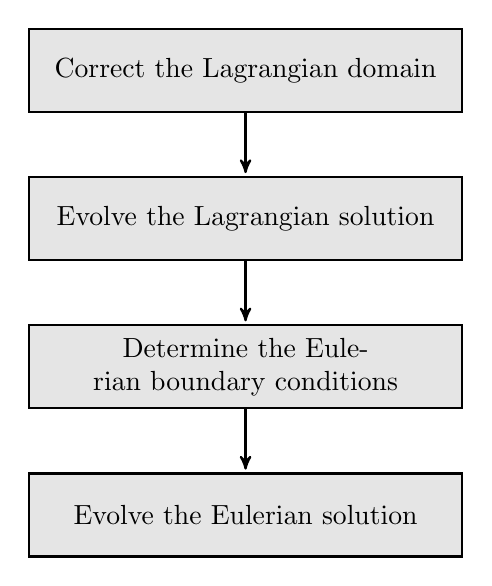
\begin{tikzpicture}
			[node distance=.8cm, start chain=going below,]
			\node[punktchain, join] (correct) {Correct the Lagrangian domain};
		    \node[punktchain, join] (evolveL) {Evolve the Lagrangian solution};
		    \node[punktchain, join] (bcE)     {Determine the Eulerian boundary conditions};
		    \node[punktchain, join] (evolveE) {Evolve the Eulerian solution};
		\end{tikzpicture}
		\caption{Flowchart of the simple coupling strategy. The flowchart shows the procedure to evolve both methods from $t_n$ to $t_{n+1}$.}
		\label{fig:flowchart_simpleCoupling}
	\end{figure}

Figure \ref{fig:flowchart_simpleCoupling} shows the overview to the simple coupling strategy. The detailed algorithm to the simple coupling strategy follows from Daeninck \cite{Daeninck2006}.

The \underline{simple coupling algorithm} can be summarized as follows:

	\begin{enumerate}
	\item \textbf{Correct Lagrangian:} Use the solution of the Eulerian domain $\Omega_E$ (in the near-wall region) to correct the solution of the Lagrangian domain $\Omega_L$ overlapping in the Eulerian domain.  
	\item \textbf{Evolve Lagrangian:} With the modified solution, evolve the Lagrangian solution from $t_n$ to $t_{n+1}$.
	\item \textbf{Determine Eulerian boundary conditions:} Use the Lagrangian solution of $t_n$ and $t_{n+1}$ to determine the boundary conditions of the Eulerian domain.
	\item \textbf{Evolve Eulerian:} With the boundary condition, evolve the Eulerian solution from $t_n$ to $t_{n+1}$.
	\end{enumerate}
	
This is the basic approach for coupling the Eulerian method in the Eulerian domain $\Omega_E$ with the Lagrangian method in the Lagrangian domain $\Omega_L$ without the iterative Schwartz algorithm. In addition, the second difference between the classical hybrid method is that the Lagrangian method handles the boundary conditions differently. Typically during the evolution process of the Lagrangian domain, vorticity is shed from body. However, in this coupling strategy, the Lagrangian method under-resolves the boundary and cannot be used to resolve the vorticity flux. Instead, we use the Eulerian method to resolve the boundary and interpolate the newly generated vorticity into the Lagrangian domain.

However, there as some \underline{assumptions} that we must satisfy, for this coupling strategy to be valid:

	\begin{enumerate}
	\item At $t_n$, before the evolution of both method to $t_{n+1}$, the Lagrangian solution matches Eulerian solution at the near-wall region.
	\item After the evolution to $t_{n+1}$, the deviation of the Lagrangian solution (due to lack of vorticity flux at Lagrangian boundary), is minimal.
	\item Even though the Lagrangian domain is under-resolved in the near-wall region, it should be able to provide accurate boundary conditions for the Eulerian external boundary.
	\end{enumerate}


\section{Verification and Validation Test Cases}

The test-cases that are used for this thesis are summarized as given:

	\begin{description}
	\item[Lamb-Oseen vortex] \cite{Lamb1993} \cite{Tryggeson2007} \hfill\\
	Lamb-Oseen vortex test case is an analytical solution derived from the diffusion equation, and is a test case for unbounded flow (without any wall). This is the first model that will be used to validate the Lagrangian method and Eulerian method separately. This test case focuses on the diffusion of the vortcity is an ideal to verify and validate the convection and diffusion of the vorticity.
	\item[Clercx-Bruneau dipole] \cite{Clercx2006}\hfill\\
	The Clercx-Bruneau dipole test case is the simple case of dipole colliding with a wall and is used to verify the coupling of the methods. This test cases focuses on the generation of vorticity from the wall and is ideal to verify and validate the coupling.
	\item[Impulsively started cylinder] \cite{LEONARD1995} \cite{Chang2006} \cite{Chassaing1986} \cite{Lecointe1985}\hfill\\
	The impulsively started cylinder test case focuses on the forces acting on the cylinder. This test case is used to verify and validate the lift and drag evolution of the cylinder exposed to free-stream flow.
	\item[Elliptic Airfoil] \cite{Nair1997}\hfill\\
	The elliptic airfoil test cases focuses on the flow separation past a lifting body. The elliptic airfoil is pitched at high angle of attack and the flow past the airfoil is comparatively unsteady and undergoes phenomenons such as laminar separation bubble, flow separation and karman vortex shedding from the trailing edge of the airfoil. This helps us ensure coupling process is sound for complex flow phenomenons.
	\end{description}

%\todo{add picture here}
\section{Methodology}
The initial steps of the development of the hybrid vortex methods is as follows:

	\begin{itemize}
	\item Develop the vortex particle method
	\item Validate the vortex particle method against a Lamb-Oseen convection test case.
	\item Develop the vortex panel method to deal with the boundaries for the vortex particle calculation. 
	\item Validate the vortex panel method by solving a potential flow around a cylinder.
	\item Develop the grid solver that is based on the Finite Element method. 
	\item Validate the grid solver against test cases: impulsively starting cylinder, dipole-Wall interaction.
	\end{itemize}

Once all the components have been validated, the methods will be coupled and validated against similar test cases.

	\begin{itemize}
	\item Couple vortex particle, vortex panel and grid solver together.
	\item Validate it with the previous generated test case solution.
	\item Introduce more complicated phenomenons: multiple geometry (i.e multiple grid meshes) and moving boundaries, if it feasible in the constraints of a master thesis.
	\end{itemize}

If the coupled solver has been validated with the test cases, the final step will be to simulated the flow around a VAWT and investigating the performance vs. numerical and experimental data.

%\subsection{Project Plan}

\section{Thesis Outline}

\todo{Update this section}

%\section{Research question}
%\label{sec:ResearchQuestion}
%
%\section{Research objective}
%\label{sec:ResearchObjective}
%
%\section{Importance of study}
%
%\section{Scope of thesis}
%\label{sec:scope}
%
%\section{Structure of the report}
%\label{sec:Structure of the report}

%

    % Chapter 2 : Lagrangian Domain: Vortex Particle Method
  	\chapter{Lagrangian Domain: Vortex Particle Method}
\label{ch:theory}

To model the flow around a VAWT, several approaches can be taken, Vermeer at al. (2003) \cite{Vermeer2003} have also summarized in their paper. The two main approaches of investigating the flow is either employing a numerical method to simulate the flow or through experimental simulations.

Leishman (2006) \cite{leishman2006principles} has shown that there are several simplified, efficient numerical tools that can be used to model the performance of a VAWT. Methods such as actuator disk theory and blade element momentum theory and deals with simplified Navier-Stokes equations and is very useful to evaluate the trend of certain design parameter. However, as they are highly simplified, complex flow phenomenons that has severe impact of the performance characteristics of the VAWT such as flow separation during dynamic stall, vortex shedding during the rotation and blade-wake interaction cannot be simulated. In order to understand them, either experimental investigation such as in wind tunnel or full Navier-Stokes simulations have to undertaken. So to understand the flow behaviour of a VAWT, several numerical research have been performed \cite{Almohammadi2013} \cite{Ferreira2007} \cite{Islam2008} \cite{Merz2012} and experimental researches by Ferreira \cite{SimaoFerreira2008} \cite{Ferreira} and others \cite{Howell2010} \cite{Mertens2003}.
\index{Actuator disk}

All the numerical method that was grid-based struggled with dealing with large number of mesh cells for high Reynolds numbers and the numerical method that employed simplified Navier-Stokes methods had to sacrifices some accuracies.The experimental investigation also come with drawbacks as they are require more financial resources and usually only feasible to model the scaled VAWTs.

This is the main relevance of the hybrid vortex particle method for the VAWT investigations. By utilizing the two methods together, the vortex particle method away from body, and Navier-Stokes solver with turbulence model in the near-body region, one will be able to tackle the challenges in an efficient manner.

Therefore, this chapter is dedicated to given an overview on the theory of the Vortex Particle Method which we will employ with coupled Navier-Stokes solver. 

\textcolor{red}{!! Add chapter outline here !!}

%------------------------------------------------------------------------------------------------------
%------------------------------------------------------------------------------------------------------
%------------------------------------------------------------------------------------------------------
\section{Introduction to Vortex Method}

\subsection{Vorticity}

\subsection{Velocity-vorticity formulation of navier-stokes equations}

Vortex methods deals with the evolution of the vorticity field in the fluid domain \cite{Cottet2000a}. So to derive the governing equations of 2-D \printAcron{Vortex Particle Method}{VPM}, we must examine the 2-D incompressible Navier-Stokes equations of a viscous fluid flow. The momentum equation is given as
\index{Vortex Method! Vortex Particle Method}

%(\textcolor{darkblue}{VPM})
%\newcommand{\printAbbreviation}[3]{#1 (#2) \nomenclature[#3]{#2}{#1}}
%\nomenclature[av]{VPM}{Vortex Particle Method}
%\printAbbreviation{Vortex Particle Method}{VPM}{av}
%\acron[t]{VPM}{Vortex Particle Method}

\begin{equation}
\frac{\partial \mathbf{u}}{\partial t} + \mathbf{u}\cdot\nabla\mathbf{u} = - \frac{1}{\rho} \nabla p + \nu \nabla^2\mathbf{u},
\label{eq:mom}
\end{equation}

with $\zeta$ characterizing the distribution of the vorticity, where $\mathbf{u}\left(\mathbf{x},t\right)$ \lsymb[f]{$\mathbf{u}$}{Velocity vector}{$[m/s]$}{u} describes the velocity field of the fluid domain, $p\left(\mathbf{x},t\right)$ \lsymb[f]{$p$}{Pressure}{$[\mathrm{Pa}]$}{p} describes the pressure field, and \gsymb[t]{$\nu$}{Kinematic viscosity}{$[m^2/s]$}{mm} and \gsymb[t]{$\rho$}{Density}{$[kg/m^3]$}{qq} are the kinematic viscosity and the density of the fluid respectively. We also have to satisfy the incompressiblity constraint given as

\begin{equation}
\nabla\cdot\mathbf{u} = 0.
\end{equation}

The governing equation of the VPM is vorticity-velocity formulation of the fluid domain. Vorticity  \gsymb[t]{$\omega$}{Vorticity}{$[1/s]$}{xx} is defined as

\begin{equation}
\mathbf{\omega} = \Delta \times \mathbf{u},
\end{equation}

and so by taking the curl of the momentum equation, we derive the vorticity transport equation, 

\begin{equation}
\frac{\partial \omega}{\partial t} + \mathbf{u}\cdot\nabla\omega = \nu \nabla^2 \omega.
\end{equation}

\subsection{Viscous splitting algorithm}

The VPM deals with the evolution of the vorticity feild using the viscous splitting (or Fractional step) method \cite{Cottet2000a}. The time stepping of the vorticity is done by dealing the viscous and the inviscid part of the transport equation separately,

\index{VPM}

\begin{itemize}
\item convection:
\begin{equation}
\frac{\partial\omega}{\partial t} + \mathbf{u}\cdot\nabla\omega=0;
\label{eq:convectionEulerian}
\end{equation}
\item diffusion:
\begin{equation}
\frac{\partial\omega}{\partial t} = \nu\nabla^2\omega.
\end{equation}

\end{itemize}

The first substep of the evolution deals which the convection of the vorticity. The diffusion of the vorticity field is evaluated by modifying the vorticity field after the convection. 
%This equation is known as the vorticity transport equation \cite{LEONARD1995}. To solve this equation, we employ a viscous splitting algorithm, where the evolution of the vorticity field is convection and the diffusion of the vorticity field is handled in separate sub-steps.

%There are several advantage to this type of evolution. As the convection and diffusion are handled separately, there is minimum dispertion during the convection and furthermore, the is no restriction of the advection CFL number \cite{Wee2006}.


%------------------------------------------------------------------------------------------------------
%------------------------------------------------------------------------------------------------------
%------------------------------------------------------------------------------------------------------
\section{Spatial Discretization: Generation of Vortex Blobs}


\subsection{Discrete form of vorticity field}
The spatial discretization of the fluid domain is done by representing the vorticity field in $N$ Lagrangian vortex particles. This is done by dividing the fluid domains into cells where the circulation of the region is assigned to the particle. This gives 

\begin{equation}
\omega\left(\mathbf{x},t\right) \simeq \omega^h\left(\mathbf{x},t\right) = \sum_{p}\Gamma_p\left(t\right)\zeta_{\sigma}\left[\mathbf{x}-\mathbf{x}_p\left(t\right)\right],
\end{equation}

\subsection{Mollified vortex kernels}

where $\Gamma_p$ \gsymb[f]{$\Gamma$}{Circulation}{$[m^2/s]$}{c} is the estimate of the circulation around the particle $\mathbf{x}_p$ \lsymb[f]{$\mathbf{x}_p$}{Position vector}{[-]}{x} with core size \gsymb[t]{$\sigma$}{Core size}{[$m$]}{rr}. We must not that $\omega^h$ is an approximation to $\omega$ of the fluid.

Due to the non-zero size of the vortex elemnts, it is refered to as vortex blobs. The advantage of the vortex blobs is that the with a smooth distribution of the vorticity, the singularity disappears and so numerical instability does not happen when blobs get too close to each other. 

An ideal choice for a cutoff function is a Gaussian distribution. Gaussian kernels satisfy the requirement for smooth distributon ad decays quickly. The Gaussian kernel is defined as

\begin{equation}
\zeta_{\sigma} = \frac{1}{k\pi\sigma^2}\exp\left(\frac{-\left|\mathbf{x}\right|}{k\sigma^2}\right),
\end{equation}

where $k$ is 1, 2 or 4 and determines the width of the kernel.

\begin{figure}
	\centering
	\includegraphics[width=0.7\textwidth]{figures/theory/gaussianKernel.pdf}
	\caption{Vortex blob with Gaussian distribution: [$k=2$,$\sigma=1.0$]}
\end{figure}


\subsection{Beale's correction: Iterative circulation processing scheme}


\subsection{Error in blob initialization}

%------------------------------------------------------------------------------------------------------
%------------------------------------------------------------------------------------------------------
%------------------------------------------------------------------------------------------------------
\section{Convection of vortex blobs}


\subsection{Biot-savart law}
The vortex transport equation evaluated using the viscous splitting algorithm. For vortex methods, it is ideal to express the equation \ref{eq:convectionEulerian} in Lagrangian form,

\begin{equation}
\frac{\mathrm{d}\mathbf{x}_p}{\mathrm{d}t} = \mathbf{u}\left(\mathbf{x}_p\right),
\end{equation}
with
\begin{equation}
\frac{\mathrm{d}\omega_p}{\mathrm{d}t} = 0.
\end{equation}

The velocity field can be decomposed using the Helmoltz decomposition,
\begin{equation}
\mathbf{u} = \mathbf{u}_{\infty} + \mathbf{u}_{\omega}
\end{equation}
with \lsymb[t]{$\mathbf{u}_{\infty}$}{Free-stream velocity}{$[m/s]$}{ul} as the free-stream velocity, \lsymb[t]{$\mathbf{u}_{\omega}$}{Vortical velocity}{$[m/s]$}{uxx} as the velocity of the vortical part of the flow.


The velocity can be related to the vorticity using the Biot-Savart law
\begin{equation}
\mathbf{u} = \mathbf{u}_{\infty} + \mathbf{K}\star\omega,
\end{equation}
\begin{equation}
\mathbf{u} = \mathbf{u}_{\infty} + \mathbf{K}\star\omega,
\end{equation}

where the $\star$ represents convolution of the kernel $\mathbf{K}_p$ given by

\begin{equation}
\mathbf{K}_p = \frac{1}{2\pi\left|\mathbf{x}\right|^2}\left(-x_2,x_1\right).
\label{eq:GreensKernel}
\end{equation}

The advantage of discretizing and evaluting the vorticity field in this form is that vortex elements are only needed where the vorticity is nonzero. This means that the vortex elements inherently adapts to domain of interest and does not require simulation of region where nothing happens. From equation \ref{eq:GreensKernel}, we see that it has a singularity when the particles approach each other and so to overcome this we can mollify the kernel using a smooth cutoff function \gsymb[t]{$\zeta$}{Smooth cutoff function}{[-]}{ff}. So the mollified kernel $\mathbf{K}_{\epsilon}$ is given as 

\begin{equation}
\mathbf{K}_{\epsilon} = \mathbf{K} \star \zeta_{\epsilon}.
\end{equation}

\subsection{Remeshing scheme: Treating lagrangian grid distortion}

%------------------------------------------------------------------------------------------------------
%------------------------------------------------------------------------------------------------------
%------------------------------------------------------------------------------------------------------
\section{Diffusion of Vortex Methods}

\subsection{Vorticity diffusion techniques}

\subsection{Modified remeshing for treating diffusion}

%\subsection{Convergence of the viscous vortex method}
%------------------------------------------------------------------------------------------------------
%------------------------------------------------------------------------------------------------------
%------------------------------------------------------------------------------------------------------
\section{Boundary conditions at solid boundary}

\subsection{Boundary integral equations}

\subsubsection{Linked boundary conditions}

\subsection{Panel method for treating no-slip boundary condition}

\subsection{Convergence study of panel method}

\section{Simulation acceleration techniques}

\subsection{Fast multi-pole Method}

\subsection{Parallel computation in GPU}

\section{Validation of lagrangian method}

\subsection{Lamb-oseen vortex at $Re=100$}

\subsection{Convection of Clercx-Bruneau dipole at $Re=625$}

\section{Summary}



%\section{Convection step}
%
%The convection step of the vorticity transport equation is define by following equation
%
%\begin{equation}
%\frac{d\mathbf{x}_i}{dt} = \mathbf{u}_i\left(\mathbf{x}_1,\mathbf{x}_2,...,\mathbf{x}_N,t\right),
%\end{equation}
%
%and we have to ensure that the circulation is conserved,
%
%\begin{equation}
%\frac{d\Gamma}{dt} = 0.
%\end{equation}


	% Chapter 3: Eulerian Domain: Finite Element Method
	\chapter{Eulerian Domain: Finite Element Method}
\label{ch:eulerian}
	\lsymb[f]{$\mathcal{T}_h$}{Finite Element mesh}{-}{th}		
	\lsymb[f]{$T$}{Cell of Finite Element mesh}{-}{t}			
	
	\lsymb[f]{$v$}{Test function}{-}{v}				
	\lsymb[f]{$V$}{Trial vector function space}{-}{vte}				
	\lsymb[f]{$\hat{V}$}{Test vector function space}{-}{vtr}					
	\gsymb[f]{$\Omega$}{Fluid domain}{-}{x}	
	\gsymb[f]{$\Omega_E$}{Eulerian fluid domain}{-}{xe}	
	\gsymb[f]{$\Omega_L$}{Lagrangian fluid domain}{-}{xl}	
	\gsymb[f]{$\partial \Omega$}{Boundary of the domain $\Omega$}{-}{xdd}	

%------------------------------------------------------------------------------------------------------
%------------------------------------------------------------------------------------------------------
%------------------------------------------------------------------------------------------------------
%\section{Purpose of eulerian domain}
Standard \printAcron{Computation Fluid Dynamics}{CFD} method discretizes the fluid into smaller regions, known as grids, and solves the set of Navier-Stokes equations in this region. This type of formulation is referred to as an Eulerian method, as we are evaluating the change of flow property in a given volume.

For the hybrid method, we use the Navier-Stokes grid formulation in the near-body region. The advantage of using the Eulerian method at this region is that it is much more efficient in resolving the boundary layer than the Vortex Particle Method. We can directly enforce the wall boundary condition at the wall boundary of the Eulerian domain, solving the problem of vorticity generation of the body. In the hybrid coupling strategy, we can then interpolate this newly resolved near-wall solution on to the Lagrangian domain, where the vortex blobs can efficiently evolve the particles.

The various approaches to solve the fluid dynamics problem from a Eulerian reference frame. \indexAcron{Finite Volume Method }{FVM}, \indexAcron{Finite Difference Method}{FDM}, and \indexAcron{Finite Element Method}{FEM} are the common choice for solving the Navier-Stokes problem and differ by the way they approach to solve the problem. FVM divides the domain into volumes where it enforces the conservation of mass and momentum in each sub-domains. FDM divides the domain into nodes and use local Taylor expansions to approximate the partial differential equations. FEM divides the domain into elements and solves the problem using variational calculus. So in the end, the choice of Eulerian method does not have a direct impact on the coupling with the Lagrangian method as the purpose of the Eulerian method is only to efficiently, and accurately resolve the near-body region of the body.

We have decided to use the FEM packages provided by the \fenics project as they have be already implemented efficient, multi-threaded algorithms for solving the partial differential equation. Furthermore, they provide extensive features for future developments such as adaptive mesh refinement, fluid-structure interaction, and efficient computation of turbulent flow.

\section{Introduction to Finite Element Method}

\printAcron{Finite Element Method}{FEM} is numerical method to solve for the solution of a given partial differential equation. It is solved by describing it as a variation problem, giving us an approximate solution for the boundary value problem \cite{Brenner2002}. So the FEM approximates the unknown variables and converts the partial differential equations to a set of algebraic equations, which makes them easier to solve. It was traditionally used for solid mechanics (e.g for the analysis of aircraft structures \cite{RAO2011}), but have since then used to solve fluid dynamics problems \cite{Guermond2006a} \cite{Johnston2004a} \cite{Guermond2003a}.

\subsection*{Finite element discretization}

The finite element solves problem by dividing the domain of interest into smaller, simpler regions known as ``elements". These ``elements" are connected at the joints which are called nodes or nodal points. We use these sets of node and elements to represent the actual variation in the field (such as the displacement, the velocity, the pressure or the temperature) using simple functions, known as the basis functions. Thus, we have transformed the domain of interest into finite number of \indexAcron{Degrees of Freedom}{DOF}. We combine the set of equations of the element into a global system of equations to solve for the unknown.

	\begin{figure}[b]
	\centering
	\includegraphics[width=0.4\linewidth]{./figures/eulerian/finiteElementDefinitions.pdf}
	\caption{A two-dimensional finite element geometry. The cell represents the area of the element, and vertices are the edges of the cell.}
	\label{fig:finiteElementDefinitions}
	\end{figure}

A finite element discretization in 2-D can be seen in figure \ref{fig:finiteElementDefinitions}. The figures shows two connected elements, where the cells represent the area of the element, and the vertices of the cell represents the nodes of the element. The finite number of cells $\mathcal{T}_h = \{T\}$ of the fluid domain $\Omega$, together makes the mesh of the Eulerian domain. As shown in figure \ref{fig:finiteElementDefinitions}, the cells of the finite element in 2-D, are made of simple geometrical shapes such as triangles or quadrilaterals. There are two approaches to discretize the domain: structured or unstructured mesh. The structured mesh has cells oriented in a structured pattern, and is the simplest approach in discretizing the mesh. The advantage of such a discretization is that it is possible to make a simple data structure which can be used to perform efficient computation. The downside to such discretization is that the mesh quality deteriorates as one increases the complexity of the domain. However, the FEM enables us to perform an unstructured discretization of the domain, as shown in figure \ref{fig:cylinderFiniteElementDiscretization}. The figure shows the unstructured discretization of the fluid domain around the cylinder $\Omega_E$, connecting the rectangular outer boundary of the fluid to the circular no-slip boundary of the body in a simple fashion. This shows that even though the unstructured method formulation is more complicated that the structured formulation, we have the advantage that the mesh quality does not deteriorate as the domain becomes more complex.

There are several algorithms for mesh generation. The standard approach is to employ the Delaunay triangulation method derived from the Voronoi diagram concept \cite{Carey1997}. This divides the domain into a set of triangles, as shown in figure \ref{fig:cylinderFiniteElementDiscretization}. This type of mesh generation allows us to connect different shapes of boundary with each other. Furthermore, this triangulation method be controlled by predefining the boundary element nodes using a transfinite interpolation.

\begin{figure}[t]
        \centering
        \begin{subfigure}[b]{0.5\textwidth}
                \includegraphics[width=\textwidth]{figures/eulerian/cylinderPreDelauney-crop.pdf}
                \caption{Fluid domain $\Omega_E$ around the cylinder}
                \label{fig:cylinderPreDelauney}
        \end{subfigure}%
        ~ %add desired spacing between images, e. g. ~, \quad, \qquad etc.
          %(or a blank line to force the subfigure onto a new line)
        \begin{subfigure}[b]{0.5\textwidth}
                \includegraphics[width=\textwidth]{figures/eulerian/cylinderDelauney-crop.pdf}
                \caption{Delaunay triangulation of the fluid}
                \label{fig:cylinderDelauney}
        \end{subfigure}
        \caption{Delaunay triangulation of the fluid around a cylinder resulting in unstructured mesh with controllable cell sizes.}
        \label{fig:cylinderFiniteElementDiscretization}
\end{figure}	

\subsection*{Finite element function and function space}

The finite element is defined using a triple ($T, \mathcal{V}, \mathcal{L}$), as defined Ciarlet \cite{Ciarlet1972b} and used by the \fenics Project \cite{Logg2012b}. The domain $\Omega$ is divided into cells $T$, the space $\mathcal{V} = \mathcal{V}(T)$ is a finite dimensional function space on $T$ of dimension $n$, and $\mathcal{L} = \left\{ \ell_1,\ell_2,...,\ell_n \right\}$ is the set of degrees of freedom forming the basis for the dual space $\mathcal{V}'$ of $\mathcal{V}$.

When the domain $\Omega$ is divided into cells $T$, we can define the function and the function space of the finite element problem. For each cell, a local function space $\mathcal{V}$ can be defined to collectively construct the global function space $V$. Any given function $u \in V$ is a expressed in a linear combination of basis functions $\{\phi_1,\phi_2,...,\phi_N\}$,  of the function space $V$, 
	\begin{equation}
	u(x) = \sum_{j=1}^N U_j\phi_j(x).
	\end{equation}

There are several types of finite element families: the Brezzi-Douglas-Marini, the Crouzeiz-Raviart, the Discontinuous Lagrange, the Hermite, and the Lagrange elements \cite{Logg2012b}. Each has its own advantage such as the Discontinous Lagrange, or \indexAcron{Discontinous Galerkin}{DG} element consists of discontinuous functions, which was originally introduced for solving hyperbolic problem by Reed and Hill in 1973 \cite{Reed1973a}. The method was able to conserve mass at each element, had a high-order accuracy, and was robust in solving the advection problem. However for the current problem, we will rely on the Lagrange elements, also known as the \indexAcron{Continuous Galerkin}{CG}, which are based on the Lagrange polynomials \cite{Chen2011}. These elements are widely used and are the simplest to implement for our project. 

Lagrange elements belong to the space $H^1$, which a Sobolev space containing functions $u$ such that $u^2$ and $\left|\nabla u\right|^2$ have finite integral in the domain $\Omega$ \cite{Logg2012b}. The Lagrange element uses point evaluation for the degrees of the freedom, where a DOF in $(x,y)$ denotes the point evaluation of the function $u$, $\ell(u) = u(x,y)$. We can have a Lagrange elements of various orders $q = 1, 2,...$, where $q$ is the degree of the Lagrange polynomial $\mathcal{P}_q$ on the domain at $T$. For the 2-D case, the dimension $n$ of the finite element is given as,
	\begin{equation}
	n(q) = \frac{1}{2}(q + 1)(q + 2).
	\end{equation}

For $q=1$, we have a simple Lagrange element $\mathrm{CG}_1$, known as the Courant triange \cite{Courant1943}, with $3$ DOFs. For a higher order finite element, we can set $q=2$, giving us a Lagrange element $\mathrm{CG}_2$ with $6$ DOFs per cell. Figure \ref{fig:continuousGalerkin} shows the two Lagrange triangles $\mathrm{CG}_1$ and $\mathrm{CG}_2$ for $q = 1$ and $q=2$ respectively. The Courant triangle has the DOFs located at the vertices of the cell, and the higher order $\mathrm{CG}_2$ has $3$ additional DOFs, all located midway between the vertices. To describe our Eulerian problem of our hybrid scheme, we will rely on the $\mathrm{CG}_1$ and $\mathrm{CG}_2$ Lagrange elements.

	\begin{figure}[t]
	\centering
	\includegraphics[width=0.6\linewidth]{./figures/eulerian/continuousGalerkin.pdf}
	\caption{The Lagrange $\mathrm{CG}_q$ triangle for $q = 1, 2$. The triangles have $3$ and $6$ DOFs respectively ({\color{black}{$\bullet$}}, black dot).}
	\label{fig:continuousGalerkin}
	\end{figure}



\subsection*{Variational formulation}
\label{subsec:variationalProblem}

To solve a basic problem such as a Poisson equation numerically, we need to convert it into a variational problem. The methodology is followed from the \fenics tutorial provide by Langtangen \cite{Logg2012b}. A 1D Poisson problem is given as,
	\begin{equation}
	\begin{aligned}
	- \nabla^2 u(x) &= f(x), \qquad x\ \mathrm{in}\ \Omega,\\
	u(x) &= u_0(x), \qquad x\ \mathrm{on}\ \partial\Omega.
	\end{aligned}
	\label{eq:poissonEq}
	\end{equation}
	
We can transform equation \ref{eq:poissonEq} into a variational form by multiplying it with a test function $v$, and integrating it over the domain $\Omega$,
	\begin{equation}
	- \int_{\Omega} \left(\nabla^2 u\right)v\ \mathrm{d}x= \int_{\Omega} fv\ \mathrm{d}x, \qquad \forall\ v \in \hat{V}.
	\label{eq:poissonEqVariationFormA}
	\end{equation}

In variational form equation \ref{eq:poissonEqVariationFormA}, the function $u$ is known as the trial function, and is what we are trying to approximate. The trial function $u$ lies in the trial function space $V$, and the test function $v$ lies in the test function space $\hat{V}$. When performing integration by parts, the test function $v$ is required to be zero at regions where $u$ is known. So, the additional terms cancel and we get,

	\begin{equation}
	- \int_{\Omega} \nabla u \nabla v\ \mathrm{d}x= \int_{\Omega} fv\ \mathrm{d}x \qquad \forall\ v \in \hat{V}
	\label{eq:poissonEqVariationFormB}
	\end{equation}

This form is referred to as the ``weak-form" of the original Poisson equation and is valid for all $v$ in the trial space $\hat{V}$. An inner product of any two function $f$ and $g$ in domain $Omega$ is defined as,
	\begin{equation}
	\langle f,g \rangle = \int_{\Omega}fg\ \mathrm{d}x,
	\end{equation}
so we can simplify equation \ref{eq:poissonEqVariationFormB} to,
	\begin{equation}
	\langle \nabla u,\nabla v \rangle = \langle f,v \rangle, \qquad \forall\ v \in \hat{V}.
	\end{equation}

In order to solve this continuous problem numerically, we must transform it into discrete variational problem,

	\begin{equation}
	-\langle \nabla u_h, \nabla v \rangle = \langle f, v \rangle \qquad \forall\ v \in \hat{V}_h \subset \hat{V},
	\label{eq:poissonEqDiscreteVariational}
	\end{equation}

where $u_h$ is the discrete function in the discrete space $V_h$ which is a subset of $V$, and the discrete function space $\hat{V}_h$ is a subset of $\hat{V}$. A common choice for the function space is linear triangular element with three nodes (Courant triangle), as shown in figure \ref{fig:continuousGalerkin}, where $\hat{V}_h$ and $V_h$ are described by piecewise linear functions of the triangle. At the boundary, the functions in the test space is zero, whereas the functions in the trial space is equal the boundary condition $u_0$.  The equation \ref{eq:poissonEqDiscreteVariational} can be simplified as,
	\begin{equation}
	a\left(u,v\right) = L(v),
	\label{eq:weakForm}
	\end{equation}
where,
	\begin{equation}
	a\left(u,v\right) = - \langle \nabla u, \nabla v \rangle,
	\end{equation}
and
	\begin{equation}
	L(v) = \langle f,v \rangle.
	\end{equation}

The variable $a(u,v)$ and $L(v)$ is the denoted as the bilinear and linear form, respectively. For simplicity, we will ignore the discrete notation (i.e $\{\cdot\}_h \rightarrow \{\cdot\}$). To solve for the discrete solution we substitute,	
	\begin{equation}
	u = \sum_{j=1}^{N} U_j \phi_j,
	\label{eq:trialDiscrete}
	\end{equation}
the linear combination of the basis function $\phi_j$, spanning the function space $V$, into $a\left(u,v\right)$. The test function is linear combination of the basis function $\hat{\phi}_i$, spanning the test space $\hat{V}$, which is defined as
	\begin{equation}
	v=\sum_{i=1}^{N} \hat{\phi}_i.
	\label{eq:testDiscrete}
	\end{equation}
	
The test function $v$ is taken to be zero at the boundary and one everywhere else. Substituting equation \ref{eq:trialDiscrete} and \ref{eq:testDiscrete} into equation \ref{eq:weakForm} gives,
	
	\begin{equation}
	\sum_{j=1}^N a(\phi,\hat{\phi}_i)\ U_j = L(\hat{\phi}_i).
	\end{equation}

Thus, we have to solve a linear system of equations given as,

	\begin{equation}
	\mathbf{A}U = b,
	\label{eq:linearSysOfEq}
	\end{equation}	
	
where $\mathbf{A}_{ij} = a(\phi_j,\hat{\phi}_i)$ is the coefficient matrix, and $b$ is the \printAcron{Right-Hand Side}{RHS} containing the knowns of the problem.
 	
%------------------------------------------------------------------------------------------------------
%------------------------------------------------------------------------------------------------------
%------------------------------------------------------------------------------------------------------
\section{Solving the Finite Element problem}

To solve this linear system of equations, equation \ref{eq:linearSysOfEq}, we used the \fenics Project that had implemented a comprehensive library of finite elements,, high performance linear algebra, and a scripting interface in \textsc{Python}. The scripting interface in \python enabled us to perform computation similar to a \matlab interface, where we could focus on the development of the algorithm, with minimal time spend on the code generation and the debugging process. The \dolfin library from the \fenics Project was used in python to define the finite element problem. 

In order to generate the mesh of the fluid domain, we used \gmsh, a three-dimensional finite element mesh generator which proves a fast, light and user-friendly meshing tools.

\subsection{Introduction to FEniCS Project}

The \fenics Project is a collaborative work of various universities, that developed tools to perform automated finite element algorithms that can be used to solve the solutions of the partial differential equation. It was a project originated in 2003 with the research collaboration of University of Chicago and Chalmers University of Technology with Logg,  Mardal, and Wells \cite{Logg2012b}. Since then, it has been expanded to various institutes such as Royal Institute of Technology, Simula Research Laboratory, University of Cambridge, and Delft University of Technology.

	\begin{figure}[p]
	\centering
	\includegraphics[width=0.5\linewidth]{./figures/eulerian/dolfinExampleFigure-rotated270.pdf}
	\caption{\dolfin VTK plot of the Poisson solution, given by the problem, source code listing \ref{lst:pycode-poisson}.}
	\label{fig:dolfinExampleFigure}
	\end{figure}

	\begin{listing}[p]
	\inputminted[fontseries=courier,obeytabs,fontsize=\footnotesize,mathescape,linenos,numbersep=5pt,frame=lines,framesep=2mm,xleftmargin=20mm,xrightmargin=20mm]{python}{figures/eulerian/dolfinExample.py}
	\caption{A complete program for solving the Poisson problem and plotting the solution. The Poisson problem is given as $-\nabla^2{u} = f$, where $u_0 = \sin{x}\cdot\cos{y}$ on the boundary and $f=2$. The code is written in \python using \dolfin 1.2 library}
	\label{lst:pycode-poisson}
	\end{listing}

The consists of various libraries such as UFC, UFL, FIAT, INSTANT and mainly \textsc{Dolfin}. \dolfin is the core library aimed at automating the solution of partial differential equations using finite element method \cite{Logg2010a}. It uses automated code generation maintaining high level of mathematical expressions and internally providing efficient, multi-threaded performance using the \indexAcron{Message Passing Interface}{MPI}. It used built-in linear algebra backend such as PETSc, TRILINOS/EPECTRA, uBLAS, and MTL4.

We used the \dolfin library in \python to solve the Poisson problem, equation \ref{eq:poissonEq}. We took $f=2$ and,
	\begin{equation}
	u(x) = u_0(x) = \sin x \cdot \cos y,
	\end{equation}
on boundary $\partial \Omega$. The code generation of the finite element was automated with the \dolfin library, leaving only the explicit expression of the problem in python. The source code to the Poisson problem is listed in listing \ref{lst:pycode-poisson}, and we see that it is a direct explicit translation of the problem, with small overheads of constructing the finite element problem.

\subsection{Mesh generation using GMSH}

The proper generation of the fluid mesh is an important aspect of the Finite Element method. It is an important process, as an ill-construct mesh can be computationally very expensive, or might even problem with convergence. There have been literatures dedicated just to improve the mesh generation, for example by Hansen \cite{Hansen2005}. It focused on mesh enhancement techniques for elliptical methods, which enables to increase the quality of the data, and also the robustness of the simulation.

For the generation of the mesh, we use \gmsh, an open-source software developed by Geuzaine and Remacle \cite{Geuzaine2009b}, which has implemented a user-friendly interface and fast algorithms. The \gmsh implemented kernels that use \textsc{BLAS} and LAPACK linear algebra packages in C++ for fast computation. Furthermore, it allows for scriptability making it ideal to integrate it with our current \python code project for future automation.

\section{Solving Incompressible Navier-Stokes Equations}
The finite element method will be used to describe the Eulerian domain of the hybrid scheme. In the Lagrangian domain, we have used the vorticity-velocity $\omega-\mathbf{u}$ formulation of the Navier-Stokes to describe the evolution of the vorticity in the wake. However, in the Eulerian domain, we will use the primitive variables, the velocity-pressure $\mathbf{u}-p$ formulation of the fluid, so that we can directly enforce the no-slip Dirichlet velocity boundary condition at the wall of the body. 

\subsection{Velocity-pressure formulation}
The velocity-pressure $\mathbf{u}-p$ formulation of the fluid, is the standard formulation of the Navier-Stokes equations of the fluid dynamics problem. The 2-D incompressible Navier-Stokes equations of a fluid with unit density (i.e $\rho = 1$) is given as,
	\begin{subequations}
	\begin{align}
	\frac{\partial \mathbf{u}}{\partial t} + \mathbf{u}\cdot\nabla\mathbf{u} - \nabla \cdot \sigma &= f,\\
	\nabla \cdot \mathbf{u} = 0,
	\end{align}	
	\label{eq:2Dns}
	\end{subequations}
where $\sigma$ is the Cauchy stress tensor defined as,
	\begin{equation}
	\sigma(\mathbf{u},p) = 2\nu\epsilon(\mathbf{u}) - p\mathbf{I}.
	\end{equation}

The Cauchy stress tensor is a function of pressure $p$, the fluid kinematic viscosity $\nu$, and the symmetric gradient $\epsilon$,
	\begin{equation}
	\epsilon(\mathbf{u}) = \frac{1}{2} \left(\nabla \mathbf{u} + \nabla \mathbf{u}^{\mathrm{T}}\right).
	\label{eq:symGrad}
	\end{equation}

So the Cauchy stress tensor defines the stress at a point in fluid due to the velocity gradient and the pressure. The incompressible 2-D Navier-Stokes equations have two unknowns, the vector velocity field $\mathbf{u}$, that lies on the vector-valued function space $V$, and the scalar pressure field $p$, which lies on the scalar-valued function space $Q$. Onces we solve for both these primitive variables, we can transfer this solution on the Lagrangian domain using the hybrid scheme. The hybrid scheme that we employ for this research, requires the transfer of the vorticity field from the Eulerian domain (i.e Eulerian grid), onto the vortex particles of the Lagrangian domain.


\subsection{Determining the vorticity field}

	\begin{listing}[t]
	\inputminted[fontseries=courier,obeytabs,fontsize=\footnotesize,mathescape,linenos,numbersep=5pt,frame=lines,framesep=2mm,xleftmargin=20mm,xrightmargin=20mm]{python}{figures/eulerian/vorticity.py}
	\caption{The \textsc{python} implementation of the vorticity calculation}
	\label{lst:pycode-vorticity}
	\end{listing}

The coupling between the Eulerian to Lagrangian method is through the transfer of the vorticity field $\omega$ from the Eulerian domain to the Lagrangian vortex blobs. The vorticity field $\omega$, is defined as,

	\begin{equation}
	\omega = \nabla \times u,
	\label{eq:vorticityEq}
	\end{equation}

and is defined as the curl of the velocity field $\mathbf{u}$. The vorticity field $\omega$ is  a scalar field that lies on the scalar-valued function space $W$. As the velocity field changes every at time $t_n$, we will have to evaluate the curl of the velocity at every step, $t_n, t_{n+1}, ...$. This brings the need for calculating the vorticity in an efficient manner, as we should not have to reconstruct the problem every step. To solve this problem in a efficient manner, \textsc{FEniCS} has implemented a function that can pre-assemble (i.e pre-calculate) the fixed parameters of the problem. To do this, we must first define equation \ref{eq:vorticityEq} in the variational (integral) form,  
	\begin{equation}
	\int_{\Omega} \omega \cdot \mathbf{v}\ \mathrm{d}x = \int_{\Omega} (\nabla \times \mathbf{u},) \cdot \mathbf{v}\ \mathrm{d}x,
	\end{equation}
where $\omega = \sum_{j=1}^N \hat{\omega}_j\psi_j$, is a linear combination of basis function $\psi_j$, spanning the function space $W$. The variational form is summarized as
	\begin{equation}
	a(\omega,\mathbf{v}) = L(\mathbf{u},\mathbf{v})
	\end{equation}
where $a(\omega,v)$ contains the knowns of the problem, which are fixed during the simulation. This can be pre-calculated to optimize the problem. $(\mathbf{u},\mathbf{v})$ is the unknown of the problem which has to be recalculated every time as it is a function of the current velocity. The \textsc{python} implementation of the algorithm is show in listing \ref{lst:pycode-vorticity}. Using the \dolfin library, we can used the \texttt{assemble} function to pre-calculated the LHS of the problem (line 10). So using the algorithms of the hybrid coupling scheme, we can transfer this vorticity field of the Eulerian domain on the vortex blobs.

\subsection{Taylor-Hood finite element family for solving ICNS}
To solve the \indexAcron{Incompressible Navier-Stokes}{ICNS} problem, we must choose an appropriate finite element function spaces for the velocity $\mathbf{u}$, the pressure $p$, and the vorticity. When determining proper mix of finite elements, we have to ensure that it satisfies the Ladyzhenskaya-Babu\v{s}ka-Brezzi (LBB) compatibility condition, also known as the inf-sup compatibility condition \cite{Brezzi1991}. When using the Lagrange finite element spaces, we have to ensure that the order of the velocity $q_{\mathrm{vel}}$, is one order higher than the order of the pressure $q_{\mathrm{pres}}$,
	\begin{equation}
	q_{\mathrm{vel}} = 	q_{\mathrm{pres}} + 1.
	\end{equation}
Brezzi and Fortin \cite{Brezzi1991} showed that if both are of same order, it will result to an unstable problem. To solve the ICNS problem, we will used the Taylor-Hood family \cite{Taylor1973}, examined by Boffi \cite{Boffi1997}. The method use velocity order $q_{\mathrm{vel}} = 2$ and pressure order $q_{\mathrm{pres}} = 1$. We decided to choose this method, as it is the most conventional method, that is simple, and that shows a stable behavior.

In addition, we have to choose an appropriate function space for the vorticity field $\Omega$. As vorticity is the curl of the velocity, to reduce interpolation error during the projection of the solution, we will used function space one order lower than the velocity, $q_{\mathrm{vort}} = 1$. Table \ref{tab:eulerianFunctionTerms} shows the list of the function spaces, the finite element type and the order. In additional, we have included the variable names of the function space, trial functions and the test functions, associated to the function element that we have chosen for the problem.

	\ctable[
	    caption = {Summary of the Lagrange element $\mathrm{CG}_q$ of order $q$, that was used for solving the incompressible Navier-Stokes problem. The variable names of the function space, the trial functions, and the test functions are also tabulated together.},
	    label   = {tab:eulerianFunctionTerms},
	    pos = b,
	]{lcccc}{}{\FL
	Variable	& Finite element & Function space	& Trial function & Test function \ML
	Velocity	& $\mathrm{CG}_2$	& $V$			& $\mathbf{u}$	 & $\mathbf{v}$\\
	Pressure 	& $\mathrm{CG}_1$ 	& $Q$			& $p$	 		 & $q$\\
	Vorticity 	& $\mathrm{CG}_1$	& $X$			& $w$	 		 & $x$\LL}


\subsection{Incremental pressure correction scheme}

The algorithm to solve the Navier-Stokes problem was first demonstrated by Chorin in 1968 \cite{Chorin1968}, referred to as the Chorin's projection method or sometimes known as the non-incremental pressure correction scheme. The process relied on first computing a tentative velocity by initially neglecting the pressure in the momentum equation of the Navier-Stokes problem, equation \ref{eq:2Dns}. The velocity field is corrected by determining the pressure field satisfying a divergence free vector field. This method however does not satisfy the discrete incompressibility constraint exactly and so, Goda in 1979 \cite{Goda1979a}, introduced an improved \indexAcron{Incremental Pressure Correction Scheme}{IPCS}. The method computed the viscous term at the incremented time $(t_{n-1} + t_n)/2$, and used the stress formulation to determine the corrected pressure \cite{Logg2012b}. 

The detailed algorithms to the IPCS scheme, as demonstrated by the \fenics Project \cite{Logg2012b}, can be summarized as follows:

	\begin{enumerate}
	\item \textbf{Compute the tentative velocity:} The tentative velocity $\mathbf{u}^{\star}$ is determined by solving,
		\begin{equation}
		\begin{split}
		\langle D_t^n \mathbf{u}^{\star}, \mathbf{v} \rangle &+ \langle \mathbf{u}^{n-1}\cdot\nabla\mathbf{u}^{n-1},\mathbf{v}\rangle + \langle \sigma(\mathbf{u}^{n-\frac{1}{2}},p^{n-1}), \epsilon(\mathbf{v}) \rangle \quad \\ &\quad+ \langle p^{n-1}\hat{\mathbf{n}},\mathbf{v}\rangle_{\partial \Omega} - \langle \mathbf{v}\ \hat{\mathbf{n}} \cdot (\nabla \mathbf{u}^{n-\frac{1}{2}} )^{\mathrm{T}},\mathbf{v} \rangle_{\partial \Omega} = \langle f^n,\mathbf{v} \rangle,
		\end{split}
		\label{eq:tentativeVel}
		\end{equation}
	is valid for all $\mathbf{v} \in V$, where $\mathbf{u}^{n-\frac{1}{2}}$ is defined as,
		\begin{equation}
		\mathbf{u}^{n-\frac{1}{2}} = \frac{\mathbf{u}^{\star}+\mathbf{u}^{n-1}}{2},
		\end{equation}
	With the Dirichlet velocity boundary conditions at the boundary $\partial \Omega$, we can solve the equation \ref{eq:tentativeVel}. The additional term,
		\begin{equation}
		\langle \mathbf{v}\ \hat{\mathbf{n}} \cdot (\nabla \mathbf{u}^{n-\frac{1}{2}} )^{\mathrm{T}},\mathbf{v} \rangle_{\partial \Omega},
		\end{equation}
	is resulted from the integration by parts, when we evaluate the viscous term at $(t_{n-1} + t_n)/2$ and we use the stress formulation instead of the Laplacian formulation as done for the Chorin scheme. This difference ensures that the velocity profile at the inlet and the outlet of the domain is more accurate that the ones obtained for the Chorin scheme. 
	
	The source code for solving the tentative velocity problem is shown in listing \ref{lst:pycode-tentativeVelocity}. First, we pre-define all the terms need for the tentative velocity problem formulation (lines \numrange{3}{16}). We can also pre-assemble the LHS of the problem (line 19) outside of the time-integration loop, as it remains constant. During the time integration, we first assemble the RHS of the problem (line 26), then apply the Dirichlet velocity boundary condition (line 29) which consist of the wall boundary condition, and external Dirichlet velocity boundary condition (e.g. the free-stream). Finally, we can solve the problem using GMRES solver for solving the system of linear equations.
	
		\begin{listing}[t]
		\inputminted[fontseries=courier,obeytabs,fontsize=\scriptsize,mathescape,linenos,numbersep=5pt,frame=lines,framesep=2mm,xleftmargin=20mm,xrightmargin=20mm]{python}{figures/eulerian/tentativeVelocity.py}
		\caption{The source code for solving the tentative velocity $\mathbf{u}^{\star}$, using the equation \ref{eq:tentativeVel}}
		\label{lst:pycode-tentativeVelocity}
		\end{listing}
	
	\item \textbf{Determine the corrected pressure:} The corrected pressure $p^n$ is determined by solving,	
		\begin{equation}
		\langle \nabla p^n, \nabla q \rangle = \langle \nabla p^{n-1}, \nabla q\rangle - \langle \nabla \cdot \mathbf{u}^{\star}, q \rangle / \Delta t_n
		\label{eq:pressureCorrection}
		\end{equation}
	is valid for all $q \in Q$. We use the previously calculated tentative velocity $\mathbf{u}^{\star}$ to determine the corrected pressure. We can solve the problem using the Neumann pressure boundary condition at the pressure outlet of the domain. We define a boundary as the pressure outlet, if we do not know the velocity boundary condition at that boundary. This is true for the region were the exit flow is perturbed. However, for the coupled Eulerian method (that we will use), all the boundary conditions are available as a velocity boundary condition from the Lagrangian domain. This means that do not have to assume any pressure boundary condition.

	The source code for solving the  corrected pressure problem is shown in listing \ref{lst:pycode-correctedPressure}. As done for the tentative velocity, we formulate and pre-assemble the problems before the time loop. In the time loop, we only need to assemble the RHS, apply the boundary condition (if it exists), and finally solve for the corrected pressure. Using the corrected pressure, we can determine the corrected velocity field. 
		
		\begin{listing}[p]
		\inputminted[fontseries=courier,obeytabs,fontsize=\scriptsize,mathescape,linenos,numbersep=5pt,frame=lines,framesep=2mm,xleftmargin=20mm,xrightmargin=20mm]{python}{figures/eulerian/correctedPressure.py}
		\caption{The source code for solving the corrected pressure $p^n$ using the equation \ref{eq:pressureCorrection}}
		\label{lst:pycode-correctedPressure}
		\end{listing}
			
	\item \textbf{Determine the corrected velocity:} The corrected velocity field $u^n$ is determined by solving,
		\begin{equation}
		\langle \mathbf{u}^n, \mathbf{v}\rangle = \langle \mathbf{u}^{\star},\mathbf{v} \rangle - \Delta t_n \langle \nabla(p^n - p^{n-1}),\mathbf{v} \rangle,
		\end{equation}
	which is valid for all $\mathbf{v} \in V$. We correct the tentative velocity $\mathbf{u}^{\star}$ by the pressure difference to determine the correct velocity field. We will have to apply the Dirichlet velocity boundary condition at the boundary again, to solve for the problem.
	
	The source code of the solving the corrected pressure problem in shown in listing \ref{lst:pycode-correctedVelocity}.
	We first initialize the problem, by formulating the problem and assembling the LHS outside the time loop (line \numrange{3}{8}). In the time integration loop, we assemble the RHS, apply the velocity boundary condition and finally solve for the corrected velocity field.
	
		\begin{listing}[p]
		\inputminted[fontseries=courier,obeytabs,fontsize=\scriptsize,mathescape,linenos,numbersep=5pt,frame=lines,framesep=2mm,xleftmargin=20mm,xrightmargin=20mm]{python}{figures/eulerian/correctedVelocity.py}
		\caption{The source code for solving the corrected pressure $p^n$ using the equation \ref{eq:pressureCorrection}}
		\label{lst:pycode-correctedVelocity}
		\end{listing}
		
	\end{enumerate}
	
This algorithm was implemented using \textsc{Dolfin}'s Krylov \textsc{Gmres} solver with absolute and relative error tolerance of \num{e-25} and \num{e-12} respectively. The program structure was based on the collection of benchmark and solvers provided by the \fenics examples scripts \cite{nsbench}. The algorithm described above an explicit time marching scheme, also referred to as \indexAcron{Forward Euler}{FE}, which is the simplest time marching scheme. Therefore, for the time marching scheme to be stable, we require the CFL number satisfy the following condition:
	\begin{equation}
	\mathrm{CFL} = \Delta t_{\mathrm{max}} \frac{\lVert\mathbf{u}\rVert_{\mathrm{max}}(\nu +  \Delta h_{\mathrm{min}}\lVert\mathbf{u}\rVert_{\mathrm{max}})}{\Delta h_{\mathrm{min}}^2} \leqslant 1.
	\label{eq:cfl}
	\end{equation}
	
	\begin{figure}[t]
	\centering
	\includegraphics[width=0.7\linewidth]{./figures/eulerian/multiStep-crop.pdf}
	\caption{Eulerian multi-stepping to match the lagrangian $\Delta t_L$. The figures shows $\Delta t_L = 4 \Delta t_E$ and required $k_E = 4$ iterations to time march from $t_n$ to $t_{n+1}$.}
	\label{fig:multiStep}
	\end{figure}		
	
This gives us the direct constraint on the maximum Eulerian time step size $\Delta t_{E,\mathrm{max}}$ which is function of the $\mathrm{CFL}$ number, maximum fluid velocity in the Eulerian domain $\lVert \mathbf{u} \rVert_{\mathrm{max}}$, the fluid viscosity $\nu$ and the minimum mesh cell size $\Delta h_{min}$. When coupling with the Lagrangian method, we will see that $\Delta t_E \leqslant \Delta t_L$ (Lagrangian time step size is ideally larger than Eulerian time step size), meaning that we will have to perform $k_E$ Eulerian sub-steps to reach the Lagrangian step, figure \ref{fig:multiStep}.

\subsection{Determining the body forces}

	\begin{listing}[t]
	\inputminted[fontseries=courier,obeytabs,fontsize=\footnotesize,mathescape,linenos,numbersep=5pt,frame=lines,framesep=2mm,xleftmargin=20mm,xrightmargin=20mm]{python}{figures/eulerian/forces.py}
	\caption{The \textsc{python} implementation of the force calculation}
	\label{lst:pycode-forceCalculation}
	\end{listing}

Once we solved for flow fields, it is a common strategy to verify the results using some sort of quantities. In aerodynamics, (especially in aerospace field), we like the evaluated the lift and drag coefficient of a given geometry and compare the results to available literature. In order to determine these coefficient, we must first determines the 
friction force and the pressure force acting on the no-slip boundary, or simply put, it is the total stress tensor $\sigma$ acting on the surface of the body. The stress tensor $\sigma$ is given by
	\begin{equation}
	\sigma(\mathbf{u},p) = 2\nu\epsilon(\mathbf{u}) - p\mathbf{I},
	\end{equation}
where $\epsilon$ is the symmetric gradient, equation \ref{eq:symGrad}, and is a function of the velocity $\mathbf{u}$ and the pressure $p$ acting on the surface.The lift coefficient and the drag coefficient is computed as,
	\begin{subequations}
	\begin{align}
	L &= \int_{\partial \Omega} \left[\sigma(\mathbf{u},p) \cdot \hat{\mathbf{n}}\right]\cdot \hat{\mathbf{e}}_y\ \mathrm{d}s,\\
	D &= \int_{\partial \Omega} \left[\sigma(\mathbf{u},p) \cdot \hat{\mathbf{n}}\right]\cdot \hat{\mathbf{e}}_x\ \mathrm{d}s,
	\end{align}
	\label{eq:LiftDragEq}
	\end{subequations}
where $\hat{\mathbf{e}}_x$ and $\hat{\mathbf{e}}_y$ are the 2D unit Cartesian vectors,
	\begin{equation}
	\hat{\mathbf{e}}_x = \begin{bmatrix}
	 1 \\ 
	 0 
	\end{bmatrix}, \qquad \quad 
	\hat{\mathbf{e}}_y = \begin{bmatrix}
		 0 \\ 
		 1 
		\end{bmatrix}.\\
	\end{equation}

The lift coefficient and the drag coefficient, $C_l$ and $C_d$ respectively, is the lift and drag normalized with the dynamics pressure and reference length $c$ (in 2D), where the lift perpendicular to the free-steam and the drag is tangential to it,
		\begin{equation}
		C_l = \frac{L}{\frac{1}{2}\lVert\mathbf{u}\rVert_{\infty}^2 c},\qquad \quad
		C_d = \frac{D}{\frac{1}{2}\lVert\mathbf{u}\rVert_{\infty}^2 c}.\\
		\label{eq:LiftDragCoeffEq}
		\end{equation}


%		\begin{subequations}
%		\begin{align}
%		C_l &= \frac{L}{\frac{1}{2}\lVert\mathbf{u}\rVert_{\infty}^2 c},\\
%		C_d &= \frac{D}{\frac{1}{2}\lVert\mathbf{u}\rVert_{\infty}^2 c}.
%		\end{align}
%		\end{subequations}

\section{Validation of eulerian method}
To validate our Eulerian method, we will first investigate the problem of the Lamb-Oseen vortex. Then we will compare the results of the Clercx-Bruneau dipole collison at $Re=625$. Finally, we will investigate the problem of the Impulsively started cylinder at $Re=550$.

\subsection{Lamb-Oseen Vortex}

	\ctable[
		caption = {Summary of the parameters for the Lamb-Oseen vortex evolution.},
		label   = {tab:eulerianLambOseenParams},
		pos = t,]{lcll}{}{\FL
		
		Parameters 					& Value 	& Unit					& Description \ML
		$\Gamma_c$\T               	& 1 &\si{m^2.s^{-1}} 				& Core strength\\
		$\Omega$               		& $\left[-1,1\right]^2$ &\si{m}		& Eulerian domain bounds \\
		$\mathbf{u}_{\infty}$ 		& $\left[0, 0\right]$ &\si{m.s^{-1}} & Free-stream velocity\\
		$\nu$						& $\num{5e-4}$ &\si{kg.s^{-1}.m^{-1}}& Kinematic viscosity\\
		$ (\tau_0,\tau_f)$ 		    & \numrange{2e-3}{2.5e-3} &\si{m^2}	& Initial and final scaled viscous time\\
		$ (t_0,t_f)$ 		    	& \numrange{4}{5} &\si{s}			& Initial and final simulation time\\		
		$ h_{\mathrm{min}}$			& $\frac{1}{100}\sqrt{2}$ &\si{m}			& Minimum mesh cell size\\	        
		$ N_{\mathrm{cells}}$ 		& $200^2$ 	& -						& Number of mesh cells\\
		$ \mathrm{CFL}$								& $0.95$ & -		& CFL number\\	        	        
		$\lVert \mathbf{u} \rVert_{\mathrm{max}}$	& $1.5$	& 	\si{m.s^{-1}} & Maximum magnitude fo the velocity\\		
		$ \Delta t$ 				& $0.001$ &\si{s}					& Time step size\\
		$ N_{\mathrm{t-steps}}$ 	& 1000 & -							& Number of time integration steps\\
		$\mathrm{ID}_{\mathrm{fluid}}$ & $1$ & - & Fluid domain I.D\\
		$\mathrm{ID}_{\mathrm{ext}}$ & $3$ & - & External Dirichlet velocity boundary I.D\LL}

The Lamb-Oseen vortex is an analytical solution by Lamb and Oseen, describing the diffusion of a vortex core \cite{Tryggeson2007}. We solved the same problem as the one described in the Lagrangian validation problem \ref{subsec:lagrangianLambOseen}. 

\subsubsection*{Problem Definition}
In the Lagrangian method, the Lamb-Oseen vortex was initialized using the vorticity field as the vortex blobs carry circulation strengths. However, Eulerian domain use the primitive variables $\mathbf{u}-p$ for formulating the problem. Therefore, we use the Lamb-Oseen velocity field as the initial conditions for the problem. The velocity field is given as,
	\begin{subequations}
	\begin{align}
	u_{\theta} &= \frac{\Gamma_c}{2\pi r} \left[1-\exp\left(-\frac{r^2}{4\tau}\right)\right]\\
	u_r &= 0,
	\end{align}
	\end{subequations}
where $\Gamma_c$ is the vortex core strength, $\tau \equiv \nu t$ is the scaled viscous time, and $r$ is the distance from the core center. The parameters of the simulation is tabulated in table \ref{tab:eulerianLambOseenParams}. To make the Eulerian simulation comparable with the Lagrangian simulation, we tried to match the spatial discretization of the Eulerian domain with the Lagrangian domain. The figure \ref{fig:lambOseenDomainDefinition} shows the domain of the problem, discretized the domain $\Omega = \left[-1,1\right]^2$ in a structure grid with the number of finite element cells $N_{\mathrm{cells}}=200^2$ in $x$ and $y$ direction, minimum cell size $h=\sqrt{2}/100$. 

	\begin{figure}[t]
	\centering
	\includegraphics[width=0.5\linewidth]{./figures/eulerian/lambOseenDomainDefinition-crop.pdf}
	\caption{Eulerian domain for the Lamb-Oseen vortex problem. Figure shows the bound of the domain $\Omega = \left[-1,1\right]^2$, identified as $\mathrm{ID}_{\mathrm{fluid}} = 1$; and the boundary domain $\partial \Omega$ [{\color{plotRed}{---}}, solid red], identified as  $\mathrm{ID}_{\mathrm{ext}} = 3$, which is where the Dirichlet velocity boundary condition was applied.}
	\label{fig:lambOseenDomainDefinition}
	\end{figure}

Furthermore, the Figure \ref{fig:lambOseenDomainDefinition} also shows the boundary domains $\partial \Omega$ of the fluid domain. For the Lamb-Oseen problem, as we have the analytical solution of the velocity field for all time, we can use this solution to prescribe the external domain boundary condition. So for this problem, we only need an external Dirichlet velocity boundary condition, at the boundary domain identified as, $\mathrm{ID}_{\mathrm{ext}} = 3$. This would imply that we do not need to explicitly apply pressure boundary condition, as we already have a velocity boundary condition. With all the boundary conditions, we can evolve the initial velocity distribution of the Lamb-Oseen vortex from $t_0 = 4$ to $t_f =5$, using the IPCS algorithm described in section \ref{sec}. 

	\begin{figure}[p]
	\centering
	\includegraphics[width=0.99\linewidth]{./figures/eulerian/lambOseen_eulerian_wRelField_compressed.pdf}
	\caption{Relative error in vorticity field in logarithmic scale. Figure \textbf{(a)} shows the initial relative error in vorticity at $t=t_0$, and figure \textbf{(b)} shows the relative error in vorticity at the end of the time stepping $t=t_f$.}
	\label{fig:lambOseen_eulerian_wRelField_compressed}
	\end{figure}
	
	\begin{figure}[p]
	\centering
	\includegraphics[width=0.6\linewidth]{./figures/eulerian/lambOseen_eulerian_wRelEvolution_compressed.pdf}
	\caption{Eulerian Lamb-Oseen relative vorticity evolution}
	\label{fig:lambOseen_eulerian_wRelEvolution}
	\end{figure}

	\begin{figure}[p]
        \centering
        \begin{subfigure}[b]{0.5\textwidth}
                \includegraphics[width=\textwidth]{figures/eulerian/lambOseen_eulerianConvergence_dx_compressed.pdf}
                \caption{Lamb-Oseen dx convergence}
                \label{fig:lambOseen_eulerianConvergence_dx}
        \end{subfigure}%
        ~ %add desired spacing between images, e. g. ~, \quad, \qquad etc.
          %(or a blank line to force the subfigure onto a new line)
        \begin{subfigure}[b]{0.5\textwidth}
                \includegraphics[width=\textwidth]{figures/eulerian/lambOseen_eulerianConvergence_dt_compressed.pdf}
                \caption{Lamb-Oseen dt convergence}
                \label{fig:lambOseen_eulerianConvergence_dt}
        \end{subfigure}
        \caption{Lamb-Oseen convergence}
        \label{fig:lambOseen_eulerianConvergence}
	\end{figure}		
	

We used $CFL$ stability condition equation \ref{eq:cfl}, to determine the time step size, $\Delta t = 0.001$. The Eulerian method time steps using a \printAcron{Forward Euler}{FE} time marching and requires $N_{\mathrm{t-steps}}=1000$ time steps. During the evolution, we evaluated the growth of the error in velocity, and in vorticity between the numerical results and the analytical solution. 

\subsubsection*{Results}
As mainly we are interested in the error in vorticity, as this is the quantity which will be interpolated onto the Lagrangian domain, figure \ref{fig:lambOseen_eulerian_wRelField_compressed} shows the initial and the final relative error in vorticity over the Eulerian domain. Opposed to the Lagrangian results, figure \ref{fig:lambOseen_convection_vorticityErrorContours_compressed}, we see that initial relative error in the vorticity field is larger. This is so because, the Lagrangian domain was initialized using the vorticity, where as the Eulerian domain was initialized using the velocity. To calculate the vorticity on the Eulerian domain, we had to project curl the velocity onto the function space of vorticity $W$. This process of initialization in the finite element domain and project of the vorticity introduced additional numerical error. However, the pattern of the relative error in vorticity, is similar to the Lagrangian solution, as the highest error is localized to the core center, where we have the highest gradient in vorticity.




As the time progress, we see that the error of the problem is stable and does not increase as observed for the Lagrangian domain, figure \ref{fig:lambOseen_eulerian_wRelField_compressed}b. The growth of the relative error in velocity and vorticity can be observed in figure \ref{fig: lambOseen_eulerian_wRelEvolution}. It shows that during the evolution of the Lamb-Oseen vortex, the relative error in velocity, and vorticity is stable. We see that due to the relation of vorticity to velocity, the error in vorticity is higher that velocity. However, the stability in the error of the solution is vital as it verifies that our method is stable and robust for solving the problem.

In order to have an extensive understanding of the stability of our scheme, we investigated the convergence of the spatial and temporal discretization of the domain. To determine the convergence of space, the simulation was run for $h \approx 0.25$ to $h \approx \num{5e-3}$. Figure \ref{fig:lambOseen_eulerianConvergence_dx} shows the convergence of the relative error in vorticity, due to increase in spatial resolution. This validates that the scheme is $2^{nd}$-order in space, due to second order function space $CG_2$ for the primitive variable, velocity.

To determine convergence in time, we ran the simulation with various time steps $\Delta t = \num{5e-3}$ to $\Delta t = \num{1e-4}$). As we performed the investigation, we saw that the error in primitive variable $\mathbf{u}$, converged at an order 1, figure \ref{fig:lambOseen_eulerianConvergence}. This is true to the theory, as we are employing a $1^{\mathrm{st}}$-order Forward Euler scheme for the time integration. Thus, we have verified with the analytical solution of the Lamb-Oseen vortex that our Eulerian method is implemented according to the theory, and perform in a robust manner.
	

\subsection{Clercx-Bruneau dipole collison at $Re=625$}

The Eulerian method that we have developed here is to be used a wall-bounded Eulerian solver that can highly resolve the vorticity production of the boundary for the Hybrid method. Therefore it is vital that the vorticity interaction with the no-slip boundary is handled properly.

To determine the proper handling of the no-slip boundary, it is common practice to use a simple test of dipole colliding with the wall. In this test cases, one could observe how the no-slip boundary handles the incoming vorticity distribution and can be used to determine if the system is formulated appropriately.  Ould-salihi et al \cite{} used this case to validate their Hybrid method that couples vortex particles with finite-difference method. Cottet et al. \cite{} used the collision to tool to validate the vortex method. 

Therefore, we decided to use the Clercx-Bruneau dipole collision is a test case from Clercx and Bruneau \cite{}, where they performed a numerical study of a normal collision of a dipole with a no-slip boundary. This experiment provide extensive benchmark results for various Reynolds numbers with a Chevyshev pseudospectral numerical method. 

\subsubsection*{Problem Definition}

Unlike other dipole test cases, Clercx and Bruneau provide well-defined initial and boundary conditions for the dipole vorticity field. Furthermore, they used a vorticity distribution that was continuous, which ensures a smooth velocity field for our Eulerian method using the $\mathbf{u}-p$ formulation. The literature of the Clercx and Bruneau provided results for two different dipole-wall collision experiments: a normal collision, where there the dipole tranvels perpendicular to the wall, and a second test case of dipole collision at an angle. 

	\begin{figure}[t]
     \centering
     \begin{subfigure}[t]{0.45\textwidth}
             \includegraphics[width=\textwidth]{figures/eulerian/clercxBruneauDomainDefinition-crop.pdf}
             \caption{Clercx-Bruneau domain definition}
             \label{fig:clercxBruneauDomainDefinition}
     \end{subfigure}%
     ~ %add desired spacing between images, e. g. ~, \quad, \qquad etc.
       %(or a blank line to force the subfigure onto a new line)
     \begin{subfigure}[t]{0.45\textwidth}
             \includegraphics[width=\textwidth]{figures/eulerian/clercxBruneauDomainMesh-crop.pdf}
             \caption{Clercx-Bruneau domain mesh}
             \label{fig:clercxBruneauDomainMesh}
     \end{subfigure}

     \caption{Comparison Parameters. $N_{\mathrm{vert}} = 48k$}
     \label{fig:clercxBruneauDomain}
	\end{figure}

For this research, we decided to use the simpler case of normal collision at $Re=625$, where $Re$ is the integral-scale Reynolds number defined as,
	\begin{equation}
	Re = \frac{UW}{\nu},
	\end{equation}
where $U$ is the characteristic velocity of the flow, $W$ is half width of domain, and $\nu$ is the kinematic viscosity. We require a low Reynolds number as the Eulerian method solves an incompressible laminar The domain $\Omega$ of the problem was taken as a square with bounds $\Omega = [-1,1]^2$, as shown in figure \ref{fig:clercxBruneauDomainDefinition}. The problem is defined in a closed box, where the Eulerian domain is enclosed in a no-slip boundary $\partial{\Omega}_{\mathrm{wall}}$ where dipole will collide and interact. 

The initial conditions of the Clercx-Bruneau dipole is a smooth vorticity distribution which a positive monopole at $(x_1,y_1)=(0.1,0)$ and the negative monopole at $(x_2,y_2)=(-0.1,0)$, with each having a radius $R = 0.1$. The vorticity distribution of the combined monopole is given as,
	\begin{equation}
	\begin{split}
	\omega(\mathbf{x},0) = \quad &\hat{\omega}_1\left[1-\left(\frac{r_1}{R}\right)^2\right]\exp\left\{-\left(\frac{r_1}{R}\right)^2\right\} \\
	+\ &\hat{\omega}_2\left[1-\left(\frac{r_2}{R}\right)^2\right]\exp\left\{-\left(\frac{r_1}{R}\right)^2\right\} ,
	\end{split}
	\label{eq:clercxBruneauOmega0}
	\end{equation}
where $\hat{\omega_1} = - \hat{\omega_2} \approx 299.528385375226$ is the extremum vorticity value of the monopole at $r_1=r_2=0$. The radii $r_1$ and $r_2$ are the radial distance from the positive and the negative monopoles respectively. Figure \ref{fig:dipole_contourLine_portrait}a shows the vorticity contours of this initial vorticity distribution. The initial vorticity distribution decays at an exponential rate to zero at the no-slip boundary. This means the no-slip boundary condition is still guaranteed for the initial distribution. To initialize the problem in the Eulerian domain with $\mathbf{u}-p$, we used the velocity distribution, 
	\begin{subequations}
	\begin{align}
	u(\mathbf{x},t) & = -\frac{1}{2}\lvert\hat{\omega}_1\rvert(y-y_1)\exp\left\{-\left(\frac{r_1}{R}\right)^2\right\} + \frac{1}{2}\lvert\hat{\omega}_2\rvert(y-y_2)\exp\left\{-\left(\frac{r_2}{R}\right)^2\right\}, \\
	v(\mathbf{x},t) & = +\frac{1}{2}\lvert\hat{\omega}_1\rvert(x-x_1)\exp\left\{-\left(\frac{r_1}{R}\right)^2\right\} - \frac{1}{2}\lvert\hat{\omega}_2\rvert(x-x_2)\exp\left\{-\left(\frac{r_2}{R}\right)^2\right\},
	\end{align}
	\label{eq:clercxBruneauVel0}
	\end{subequations}
where $u$ and $v$ are the velocity in the $x$ and $y$ direction, respectively. 

The fluid domain of the Eulerian domain, show in figure \ref{fig:clercxBruneauDomainDefinition} was discretized using an controlled unstructured meshing method. From the velocity distribution, equation \ref{eq:clercxBruneauVel0}, we see that the maximum velocity in the fluid will be along the $y$-axis (i.e $x=0$). Therefore, to satisfy the $CFL$ condition equally every, we reduce the cell size where we have the maximum velocity. Furthermore, to ensure the vorticity generation at the no-slip boundary is defined accurately, we increased resolution of the mesh at the boundary. The third region where we increased the resolution is where the dipole and the wall interacts (i.e $-0.5\le{x}\le0.5$ and $0.5\le{\left|y\right|}\le1$). In the region where there is no vorticity, we do not need high resolution (i.e $0.5\le{\left|x\right|}\le1$ and $-0.5\le{y}\le0.5$). With this parameterization, we obtained an unstructured grid with number of finite element vertices $N_{\mathrm{vert}}=48k$. 

\subsubsection*{Results}
After initializing the velocity field in the discretized domain, the problem was evolved from $t=0$ to $t=2.0$ where $t$ is non-dimensionalized using $W/U$. Using the CFL condition, equation \ref{eq:cfl}, we determine that simulation required a time step size $\Delta = \num{1.25e-5}$, with a total of $160k$ time steps. Figure \ref{fig:dipole_contourLine_portrait} shows the evolution of the vorticity field at various instances ($t = 0, 0.25, 0.5, 0.75, 1.25$). During the initial stages of the simulation, the initialized dipole travels along the $y$-axis towards the bottom no-slip boundary. The weaker outer regions of the core dipole travels in the opposite direction, and for this simulation (also by Clercx and Bruneau), this evolution of the this dipole is ignored. 

The main dipole approaches the bottom boundary, where the no-slip boundary starts to generate vorticity to ensure the no-through flow, figure \ref{fig:dipole_contourLine_portrait}b. As the primary dipole approaches closer, the vorticity filament at the wall rolls up and combines with the primary dipole forming two secondary dipoles that is assymteric across the $y$-axis. Figure \ref{fig:dipole_contourLine_portrait}c shows the state of the vorticity field at $t=0.5$ after the secondary dipoles are generated. This secondary dipole initially travels away from the bottom wall and later on approaches the wall again, colliding for a second time and creating a tertiary vortex, figure \ref{fig:dipole_contourLine_portrait}d. At $Re=625$, the dipole stops convecting any further and diffuses as time progresses ($t = 1$ and $t = 1.25$).

Figure \ref{fig:vorticity_contour_comparison} compares the vorticity contours in a small part of the computation domain ($0\leqslant x \leqslant 0.6$ and $-1 \leqslant y \leqslant -0.4$) at $t = 1$. The positive vortex (solid black) is surrounded by the negative vortex (dashed black). The primary observation tells us that the overall shape of the vorticity contours is very similar to the reference data. However we see that in the present simulation, there are more iso-vorticity lines, meaning that vortex has not lost the strength.

	\begin{figure}[p]
	\centering
	\includegraphics[width=\linewidth]{./figures/eulerian/dipole_contourLine_portrait-crop.pdf}
	\caption{Vorticity contour plots of the normal Clercx-Bruneau dipole-wall collision experiment at $Re=625$ at $t = 0, 0.25, 0.5, 0.75, 1.0, 1.25$ with vorticity contour levels at -320,-200,-100,-50,-10, 10, 50, 100, 200, 320. The figure depicts positive contours [---, solid black], and negative contours [- -, dashed black].}
	\label{fig:dipole_contourLine_portrait}
	\end{figure}
	
	\ctable[
		caption = {Summary of the parameters for the Clercx-Bruneau normal collision of a dipole with a no-slip wall \cite{}.},
		label   = {tab:clercxBruneauParameters},
		pos = p,]{lcll}{}{\FL
		Parameters					& Value 				& Unit		& Description \ML
		$\Omega$               		& $\left[-1,1\right]^2$ &\si{m}		& Eulerian domain bounds \\
		$Re$  			       		& $625$ 				&-			& Reynolds number \\ 
		$U$			         		& $1$ 					&\si{m.s^{-1}}& Characteristic velocity\\		
		$W$			         		& $1$ 					&\si{m}		& Half width of the domain\\		
		$\nu$						& $\num{1.6e-3}$ 		&\si{kg.s^{-1}.m^{-1}}& Kinematic viscosity\\
		$ (x,y)_{1,2}$				& $(\pm0.1,0)$			& \si{m}    & Initial location of the dipole\\
		$ \hat{\omega}_{1,2}$		& $\pm 299.5283853752226$ & -   	& Maximum vorticity of the monopole\\
		$ (t_0,t_f)$ 		    	& $(0,2)$				& \si{s} 	& Initial and final scaled viscous time\\
		$ \mathrm{CFL}$				& $0.95$ 				& -			& CFL number\\	        	        
		$ \lVert\mathbf{u}\rVert_{\mathrm{max}}$	& $12$	& \si{m.s^{-1}}	& Maximum fluid velocity\\
		$ \Delta t$ 		    	& $\num{1.25e-5}$		& \si{s} 	& Time step size\\
		$ N_{\mathrm{vert}}$ 		& $\sim48k$ 			& -			& Number of mesh vertices\\
		$ h_{\mathrm{min}}$			& $\sim\num{3.6e-3}$ &\si{m}		& Minimum mesh cell size\\	        
		$ N_{\mathrm{tsteps}}$ 		& $160,000$				& -	     	& Number of time integration steps\\
		$\mathrm{ID}_{\mathrm{fluid}}$ & $1$ 				& - 		& Fluid domain I.D\\
		$\mathrm{ID}_{\mathrm{wall}}$ & $2$ 				& - 		& No-slip boundary I.D\LL}
	
	\begin{figure}[p]
     \centering
     \begin{subfigure}[t]{0.4\textwidth}
             \includegraphics[width=\textwidth]{figures/eulerian/VorticityContourPlot-rotated270.pdf}
             \caption{Literature}
             \label{fig:VorticityContourPlot}
     \end{subfigure}%
     ~ %add desired spacing between images, e. g. ~, \quad, \qquad etc.
       %(or a blank line to force the subfigure onto a new line)
     \begin{subfigure}[t]{0.5\textwidth}
             \includegraphics[width=\textwidth]{figures/eulerian/dipole_contourLine_t1p0-crop.pdf}
             \caption{CPresent study}
             \label{fig:dipole_contourLine_t1p0}
     \end{subfigure}
     \caption{Vorticity contour plot}
     \label{fig:vorticity_contour_comparison}
	\end{figure}	
	
To determine the variation of the fluid properties as the time progresses, Clercx and Bruneau investigated the evolution of the total kinetic energy $E(t)$, the total enstrophy $\Omega(T)$, and the total Palinstrophy $P(t)$ of the flow field. The total kinetic energy $E(t)$ of the dipolar field can be determined as,
	\begin{equation}
	E(t) = \frac{1}{2} \int\int \mathbf{u}^2(\mathbf{x},t)\ \mathrm{d}x\mathrm{d}y,
	\end{equation}
and at $t=0$, $E(0) = 2$. The total enstrophy of the flow is determined as, 
	\begin{equation}
	\Omega(t) = \frac{1}{2}\int\int\omega^2(\mathbf{x},t)\ \mathrm{d}x\mathrm{d}y,
	\end{equation}	
and can seen as the energy of the vorticity. The change in enstrophy of the field can give an insight to dissipation rate in the fluid. At $t=0$, the enstrophy of the fluid is $\Omega(0)=800$. The total Palinstrophy $P(t)$ of the flow measures the gradient of the vorticity, 
	\begin{equation}
	P(t) = \frac{1}{2}\int\int\left[\nabla\omega(\mathbf{x},t)\right]^2\ \mathrm{d}x\mathrm{d}y,
	\end{equation}
and gives an insight to generation of vorticity at the no-slip boundary. Figure \ref{fig:dipole_comparison} compare the evolution of these time dependent parameters with the reference data provided by Clercx \& Bruneau (dotted red) for $t=0.25$, $t=0.5$ and $t=0.75$. The kinetic energy, figure \ref{fig:dipole_KineticEnergy_comparison}, reduced from $E(0) = 2$ to $E(2) \approx 0.3$. At $t=0.4$, we have small kink representing the approach of the primary dipole at the wall. When plotting the reference data, we see that the variation in kinetic energy matches perfectly at $t=0.25$, $t=0.5$ and $t=0.75$.

Figure \ref{fig:dipole_Enstrophy_comparison} compares the variation in enstrophy ($\Omega$). During the initial stages, the enstrophy decreases linearly, and at $t=0.37$ there is sharp increase in the total enstrophy of the flow $\Omega(0.37) = 938.58$. This indicates the initial impact of dipole with the no-slip wall. After the impact, the enstrophy quickly drops and peaks again at $t=0.65$ reaching $\Omega = 307.04$. In addition, to the 3 data points, Clercx \& Bruneau determined the peak enstrophy of flow. Table \ref{tab:euleriandipoleCollisionComparison} compares the difference between the present study and literature and we see that there is maximum of $0.3\%$ error in time $t$ and $0.6\%$ error in enstrophy $\Omega$. Therefore, the variation in enstrophy is well represented by our Eulerian method.

Figure \ref{fig:dipole_Palinstrophy_comparison} compares the variation in palinstrophy $P(t)$. Similar to enstrophy, we can observe to peak regions at $t=0.36$ and $t=0.65$, respesenting the two collision of the dipole. During the collision, vorticity is generated from the wall to ensure no-through boundary condition, which results in a sharp increase in the gradient of the vorticity. Table \ref{tab:euleriandipoleCollisionComparison} compares the difference with the addition data provided and we see that there is maximum error of $0.3\%$ in time $t$ and $1.8\%$ in palinstrophy $P$. This is an acceptable error and tells us the generation of vorticity in Eulerian method performs according to theory.
	
Figure \ref{fig:VorticityAtBoundary} compares the vorticity along the boundary of the domain at $y=-1$ for $-0.6 \leqslant x \leqslant 0$. The solid lines represents the present data, and is compared with the dotted data obtained from the reference. The comparison is done for various time instances $t=0.4$, $t=0.6$ and $t=1.0$ and we can finally validate that the Eulerian method accurately represents vorticity generation from the wall.
	
	\begin{figure}[p]
     \centering
     \begin{subfigure}[t]{0.49\textwidth}
             \includegraphics[width=\textwidth]{figures/eulerian/dipole_KineticEnergy_comparison.pdf}
             \caption{Kinetic Energy $E(t)$}
             \label{fig:dipole_KineticEnergy_comparison}
     \end{subfigure}%
     ~ %add desired spacing between images, e. g. ~, \quad, \qquad etc.
       %(or a blank line to force the subfigure onto a new line)
     \begin{subfigure}[t]{0.49\textwidth}
             \includegraphics[width=\textwidth]{figures/eulerian/dipole_Enstrophy_comparison.pdf}
             \caption{Enstrophy $\Omega(t)$}
             \label{fig:dipole_Enstrophy_comparison}
     \end{subfigure}
     
     \begin{subfigure}[b]{0.49\textwidth}
             \includegraphics[width=\textwidth]{figures/eulerian/dipole_Palinstrophy_comparison.pdf}
             \caption{Palinstrophy $P(t)$}
             \label{fig:dipole_Palinstrophy_comparison}
     \end{subfigure}
     ~
     \begin{subfigure}[b]{0.48\textwidth}
		\includegraphics[width=\textwidth]{./figures/eulerian/VorticityAtBoundary.pdf}
		\caption{Vorticity at the boundary y = -1.}
		\label{fig:VorticityAtBoundary}
     \end{subfigure}     
     
     \caption{Comparison Parameters}
     \label{fig:dipole_comparison}
	\end{figure}

%	\begin{figure}[p]
%	\centering
%	\includegraphics[width=0.7\linewidth]{./figures/eulerian/VorticityAtBoundary.pdf}
%	\caption{Vorticity at the boundary y = -1.}
%	\label{fig:VorticityAtBoundary}
%	\end{figure}
	

	\ctable[
	    caption = {A summary of the values of the first two maxima of the enstrophy $E$ and palinsotrophy $P$ occurinng at $t_1$ and $t_2$ respectively.},
	    label   = {tab:euleriandipoleCollisionComparison},
	    maxwidth = \textwidth,
	    pos = p,
	]{ccrrrr}{\tnote{Data provide by Clercx \& Bruneau \cite{Clercx2006a}}}{\FL
	\multirow{2}{*}{Instant} & 	\multirow{2}{*}{Case} & \multicolumn{2}{c}{Enstrophy $\Omega$} & \multicolumn{2}{c}{Palinstrophy $P$}\\
	\noalign{\smallskip}\cline{3-6}\noalign{\smallskip}
			& 			& $t$ & $\Omega$ 	& $t$ & $P$\ML
	\multirow{2}{*}{$t_1$} 	& Reference\tmark[a] 	& 0.371 & 933.6 	& 0.361 & $1.39\times10^7$\\
							& Present 		& 0.370 & 938.6 	& 0.360 & $1.40\times10^7$\\
	\multirow{2}{*}{$t_2$} 	& Reference\tmark[a] 	& 0.648 & 305.2 	& 0.652 & $6.78\times10^{5}$\\
							& Present 		& 0.650 & 307.0		& 0.650 & $6.90\times10^{5}$\LL}		
%	\multirow{2}{*}{$t_1$}	& Reference cite 	& 	0.37 & 933.6 & $1.4\times10^7$\\
%							& Present 			& $\mathrm{CG}_1$ 	& $Q$			& $p$	 		 & $q$\\
%	\multirow{2}{*}{$t_1$}	& Reference cite 	& 			& $\mathbf{u}$	 & $\mathbf{v}$\\
%							& Present 			& $\mathrm{CG}_1$ 	& $Q$			& $p$	 		 & $q$\LL}

\subsection{Impulsively started cylinder at $Re=550$}

Finally, we investigated the problem of an impulsively started cylinder at $Re=550$. This validation test ensured that at the end of the simulation, we are able to determine correct forces acting on the body. 

\subsubsection*{Problem Definition}
The \indexAcron{Impulsively Started Cylinder}{ISC} test case simulates the flow around a cylinder exposed to an impulsively started free-stream flow. The test cases focuses on the unsteady behavior of the separated flow parst the cylinder. Various experimental and numerical investigation have been performed investigating the flow characterstics, and for this project we relied on the widely used and validated results of Koumoutsakos \& Leonard \cite[]. They investigated the flow around the ISC using vortex methods, and provided extensive data on the vorticity profile behind the cylinder and the evolution of the Lift and Drag.

Figure \ref{fig:ISCDomain} shows the domain definition of the ISC problem. Figure \ref{fig:ISCDomainDefinition-crop} shows the fluid domain $\Omega_E$ with an initial conditions $\mathbf{u}=0$, and $p=0$. The domain has the following boundary conditions: the no-slip wall boundary condition at $\partial \Omega_{\mathrm{wall}}$ (solid blue) $\mathbf{u}=0$, the free-stream Dirichlet velocity boundary condition at $\partial \Omega_{\mathrm{dirichlet}}$ (solid red) $\mathbf{u}_{\infty} = [1,0]$, and the pressure outlet $\partial \Omega_{\mathrm{pressure}}$ (solid green). Unlike the previous test cases we now require a pressure outlet boundary condition $\partial p/ \partial \mathbf{n} = 0$, as the velocity field behind the cylinder perturbed and therefore free-stream boundary condition cannot be applied there.

The unsteady simulation has Reynolds number $Re$ of the flow dependent on the diameter of the cylinder $D$,
	\begin{equation}
	Re = \frac{UD}{\nu},
	\end{equation}
and the time $t$ is non-dimensionalized with the radius $R$ of the cylinder,
	\begin{equation}
	T = \frac{U}{R}t.
	\end{equation}
The domain was discretized with $N_{\mathrm{vert}}=48$, with highest mesh resolutions are found near the surface of the body, and in the wake region of the body, figure \ref{fig:ISCSurfaceMesh}. The simulation was time marched with $\Delta t = \num{1e-3}$ satisfying the CFL condition prescribed (all the parameters at tabulated in table \ref{tab:ISCParameters}).

\subsubsection*{Results}
The simulation was started with an with an impulsively started free-stream boundary condition at dirichlet boundary $\partial \Omega_{\mathrm{dirichlet}}$. The problem was evolved from $t=0$ to $t=100$ with number of time steps $N_{\mathrm{tSteps}}=100000$. To validate the scheme with the reference data of Koumoutsakos \& Leonard, we investigated the evolution of the vorticity field and the evolution of the forces acting on the body.

	\begin{figure}[p]
     \centering
     \begin{subfigure}[t]{0.49\textwidth}
             \includegraphics[width=\textwidth]{figures/eulerian/ISCDomainDefinition-crop.pdf}
             \caption{Domain definition}
             \label{fig:ISCDomainDefinition-crop}
     \end{subfigure}%
     ~ %add desired spacing between images, e. g. ~, \quad, \qquad etc.
       %(or a blank line to force the subfigure onto a new line)
     \begin{subfigure}[t]{0.49\textwidth}
             \includegraphics[width=\textwidth]{figures/eulerian/ISC_mesh-crop.pdf}
             \caption{Full mesh}
             \label{fig:ISC_mesh-crop}
     \end{subfigure}

     \begin{subfigure}[t]{0.3\textwidth}
             \includegraphics[width=\textwidth]{figures/eulerian/ISC_mesh_surface-crop.pdf}
             \caption{Mesh near surface}
             \label{fig:ISC_mesh_surface-crop}
     \end{subfigure}

     \caption{ISC problem definition}
     \label{fig:ISCDomain}
	\end{figure}

	\ctable[
		caption = {Summary of the parameters for the Impulsively started cylinder test case for $Re=550$\cite{}.},
		label   = {tab:ISCParameters},
		pos = p,]{lcll}{}{\FL
		Parameters					& Value 				& Unit		& Description \ML
		$\Omega$               		& $\left[-60,100\right]\times[-60,60]$ &\si{m}		& Eulerian domain bounds \\
		$Re$  			       		& $550$ 				&-			& Reynolds number \\ 
		$\mathbf{u}_{\infty}$		& $[1,0]$ 				&\si{m.s^{-1}}& Free-stream velocity\\		
		$R$			         		& $1$ 					&\si{m}		& Radius of cylinder\\		
		$D$			         		& $2$ 					&\si{m}		& Diameter of cylinder\\		
		$\nu$						& $\num{3.6e-3}$ 		&\si{kg.s^{-1}.m^{-1}}& Kinematic viscosity\\
		$ (t_0,t_f)$ 		    	& $(0,100)$				& \si{s} 	& Initial and final non-dimensional time\\
		$ \mathrm{CFL}$				& $0.95$ 				& -			& CFL number\\	        	        
		$ \lVert\mathbf{u}\rVert_{\mathrm{max}}$	& $2.5$	& \si{m.s^{-1}}	& Maximum fluid velocity\\
		$ \Delta t$ 		    	& $\num{1e-3}$		& \si{s} 	& Time step size\\
		$ N_{\mathrm{vert}}$ 		& $\sim47k$ 			& -			& Number of mesh vertices\\
		$ h_{\mathrm{min}}$			& $\sim\num{9.7e-3}$ &\si{m}		& Minimum mesh cell size\\	        
		$ N_{\mathrm{tsteps}}$ 		& $100,000$				& -	     	& Number of time integration steps\\
		$\mathrm{ID}_{\mathrm{fluid}}$ & $1$ 				& - 		& Fluid domain I.D (gray)\\
		$\mathrm{ID}_{\mathrm{wall}}$ & $2$ 				& - 		& No-slip boundary I.D (blue)\\
		$\mathrm{ID}_{\mathrm{dirichlet}}$ & $3$ 			& - 		& Dirichlet boundary I.D (red)\\
		$\mathrm{ID}_{\mathrm{pressure}}$ & $4$ 			& - 		& Pressure boundary I.D (green)\LL}


	\begin{figure}[p]
     \centering
     \begin{subfigure}[t]{0.45\textwidth}
             \includegraphics[height=0.2\textheight]{figures/eulerian/ISC_vorticityContours_t1_ref-mod.png}
             \caption{$t=1$ Reference}
             \label{fig:ISC_vorticityContours_t1_ref}
     \end{subfigure}%
     ~ %add desired spacing between images, e. g. ~, \quad, \qquad etc.
       %(or a blank line to force the subfigure onto a new line)
     \begin{subfigure}[t]{0.45\textwidth}
             \includegraphics[height=0.2\textheight]{figures/eulerian/ISC_vorticityContours_t1-crop.pdf}
             \caption{$t=1$ Present}
             \label{fig:ISC_vorticityContours_t1-crop}
     \end{subfigure}
     
     \begin{subfigure}[t]{0.45\textwidth}
             \includegraphics[height=0.2\textheight]{figures/eulerian/ISC_vorticityContours_t3_ref-mod.png}
             \caption{$t=3$ Reference}
             \label{fig:ISC_vorticityContours_t3_ref}
     \end{subfigure}%
     ~ %add desired spacing between images, e. g. ~, \quad, \qquad etc.
       %(or a blank line to force the subfigure onto a new line)
     \begin{subfigure}[t]{0.45\textwidth}
             \includegraphics[height=0.2\textheight]{figures/eulerian/ISC_vorticityContours_t3-crop.pdf}
             \caption{$t=3$ Present}
             \label{fig:ISC_vorticityContours_t3-crop}
     \end{subfigure} 
     
     
     \begin{subfigure}[t]{0.45\textwidth}
             \includegraphics[height=0.2\textheight]{figures/eulerian/ISC_vorticityContours_t5_ref-mod.png}
             \caption{$t=5$ Reference}
             \label{fig:ISC_vorticityContours_t5_ref}
     \end{subfigure}%
     ~ %add desired spacing between images, e. g. ~, \quad, \qquad etc.
       %(or a blank line to force the subfigure onto a new line)
     \begin{subfigure}[t]{0.45\textwidth}
             \includegraphics[height=0.2\textheight]{figures/eulerian/ISC_vorticityContours_t5-crop.pdf}
             \caption{$t=5$ Present}
             \label{fig:ISC_vorticityContours_t5-crop}
     \end{subfigure}
     
     \begin{subfigure}[t]{0.45\textwidth}
             \includegraphics[height=0.2\textheight]{figures/eulerian/ISC_vorticityContours_t7_ref-mod.png}
             \caption{$t=7$ Reference}
             \label{fig:ISC_vorticityContours_t7_ref}
     \end{subfigure}%
     ~ %add desired spacing between images, e. g. ~, \quad, \qquad etc.
       %(or a blank line to force the subfigure onto a new line)
     \begin{subfigure}[t]{0.45\textwidth}
             \includegraphics[height=0.2\textheight]{figures/eulerian/ISC_vorticityContours_t7-crop.pdf}
             \caption{$t=7$ Present}
             \label{fig:ISC_vorticityContours_t7-crop}
     \end{subfigure}         

     \caption{Vorticity contours comparison}
     \label{fig:ISCS_vorticityContours_comparison}
	\end{figure}

%	\begin{figure}[p]
%     \centering
%     \begin{subfigure}[t]{0.49\textwidth}
%             \includegraphics[width=\textwidth]{figures/eulerian/ISC_dragEvolution.pdf}
%             \caption{Drag}
%             \label{fig:ISC_dragEvolution}
%     \end{subfigure}%
%     ~ %add desired spacing between images, e. g. ~, \quad, \qquad etc.
%       %(or a blank line to force the subfigure onto a new line)
%     \begin{subfigure}[t]{0.45\textwidth}
%             \includegraphics[width=\textwidth]{figures/eulerian/ISC_LongRun_dragLiftEvolution.pdf}
%             \caption{Lift}
%             \label{fig:ISC_LongRun_dragLiftEvolution}
%     \end{subfigure}
%
%     \caption{Evolution of drag and lift. }
%     \label{fig:evolutionDragLift}
%	\end{figure}
	
	\begin{figure}[p]
	\centering
	\includegraphics[width=0.7\linewidth]{./figures/eulerian/ISC_dragEvolution.pdf}
	\caption{Drag}
	\label{fig:ISC_dragEvolution}
	\end{figure}
	
	\begin{figure}[p]
	\centering
	\includegraphics[width=0.7\linewidth]{./figures/eulerian/ISC_LongRun_dragLiftEvolution.pdf}
	\caption{Lift Drag}
	\label{fig:ISC_LongRun_dragLiftEvolution}
	\end{figure}	


Figure \ref{fig:ISC_vorticityContours_t7-crop} depicts the evolution of the vorticity from $t=1\rightarrow7$. The iso-vorticity contours of the present stuyd is compared with the reference data from the literature \cite[]. At $t=1$, negative and positive vorticity is generated at the top and bottom of the cylinder, respectively and is resulted from satisfying the no-slip boundary condition. As time progress, two primary vortices are formed right behind the cylinder, increasing in shape as time progress. Comparing the vorticity contours, we can say that the shape and the geometry of the contour lines match with the literature. 

Using equations \ref{eq:LiftDragEq} to \ref{eq:LiftDragCoeffEq}, we were able to calculate the Lift and the drag force acting on the cylinder as the time progress, which we used to validate against the literature. Figure \ref{fig:ISC_dragEvolution} shows the components of the drag force (friction drag $C_{d_{\mathrm{fric}}}$, pressure drag $C_{d_{\mathrm{pres}}}$) acting on the surface of the body. At $t=0$, we have a singularity in the total drag $C_d$ acting on the body due to the impulsive start of the flow. It then plunges to $C_d=0.75$ at $t=0.8$ and peaks again near $t=3$ at $C_d=1.3$. The dotted line is the data obtained from literature and we see that the results of the simulation matches well with the literature.

A final comparison was done for the evolution of the Lift and the Drag coefficient for larger period ($t=0$ to $t=40$), which was used to determine the oscillatory behavior of the Lift and Drag. For lower Reynolds number, the vorticity field is symmetric across the $x$-axis for a long time. This meant that the oscillatory behavior of the forces starts at a much later time. Therefore, we prescribed an artificial perturbation to the problem to create an asymmetry in the vorticity field. The perturbation was performed according to Leocointe \& Piquet \cite[],
	\begin{equation}
	 u_{\mathrm{wall}} = \begin{cases}
	 0.15 & 3 \leqslant t \leqslant 3.5, \\
	 -0.25 & 3.5 \leqslant t \leqslant 5.
	 \end{cases}
	\label{eq:perturbation}
	\end{equation}
	
With this, we could ensure that we have a controlled behavior for the lift and drag, which we used to determine the amplitude and the frequency of the oscillation. Figure \ref{fig:ISC_LongRun_dragLiftEvolution} compares the evolution of the lift and drag for $t=0$ to $t=40$. We see that our numerical scheme performs very similar to the literature \cite[]. However, there is a slight difference, which is due to the under-resolution of the Eulerian domain downstream of the cylinder.

\section{Summary}

In summary, we investigated, vertified and validated the Eulerian method for the hybrid coupling scheme, and various observation of the method has been summarized as follows:

	\begin{itemize}
	\item The Eulerian method is used to highly resolve the near-body region of the fluid.
	\item We have used a Finite Element method to solve the incompressible laminar Navier-Stokes problem using the velocity-pressure $\mathbf{u}-p$ formulation.
	\item \printAcron{Incremental Pressure Correction Scheme}{IPCS} was used to solve the Navier-Stokes problem, allowing us to decouple the velocity $\mathbf{u}$ and pressure $p$ from the momentum equation.
	\item \dolfin library from the \fenics project was used to perform automated finite element algorithms for solving the partial different equations.
	\item \gmsh mesh generation tool was used to generate the unstructured mesh of the fluid domain.
	\item Once we have determined the velocity $\mathbf{u}$ and the pressure $p$ fields, we can determine the vorticity associated to the fluid using an optimized calculation algorithm.
	\item A Lamb-Oseen Vortex test case was used to verify the implementation of the Eulerian method, and concluded that the method had a $1^{\mathbf{st}}$-order convergence in time and $2^{\mathrm{nd}}$-order convergence in space.
	\item To validate the vorticity handling and the vorticity production of the no-slip boundary, we used the high-fidelity numerical test case of Clercx \& Bruneau investigation the collision of dipole with the wall at $Re=625$. Investigating the change in kinetic energy $E$, enstrophy $\Omega$, and Palinstrophy $P$, we validate that the results matched the literature. We evaluated the vorticity generated at boundary, which also showed that our numerical method handels according to theory.
	\item The final test case involved simulating an impulsively started cylinder at $Re=550$. We investigated the shed of vorticity at time progress and validated that it matched the reference data provided by Koumoutsakos \& ???. Finally, we investigated the evolution of the Lift and drag of the cylinder, and we saw that the frequency and the amplitude of the oscillation matched the theory. Therefore, our Eulerian method accurate determine the fluid behavior past an object such as the Strouhal number St.
	\end{itemize}

\subsection*{Eulerian method algorithm}

The algorithm for the Eulerian method can be summarized as follows:

	\begin{enumerate}
	\item \textbf{Mesh generation}: We generate the mesh of the fluid domain using \gmsh before the iteration.
	\item \textbf{Determine the boundary condition}: We need to determine the boundary conditions for the boundary domains: $\partial \Omega_{\mathrm{wall}}$, $\partial \Omega_{\mathrm{dirichlet}}$, $\partial \Omega_{\mathrm{pressure}}$. If we have dirichlet velocity boundary conditions for all the exterior boundaries, we do not have to apply any pressure boundary conditions at $\partial \Omega_{\mathrm{pressure}}$.
	\item \textbf{Solve the IPCS}: Using IPCS, time march from $t_n$ to $t_{n+1}$ to solve for the new velocity $\mathbf{u}$ and pressure $p$ field.
	\item \textbf{Determine the vorticity}: Using the algorithm described in \ref{??}, solve for the vorticity field $\omega$ at the time $t_{n+1}$. 
	\end{enumerate}

Once we have the well-resolved vorticity $\omega$ of the near-body region, we use it to couple it with the Lagrangian method with our Hybrid coupling scheme.


    % Chapter 4: Hybrid Eulerian-Lagrangian Vortex Particle Method
   	\chapter{Hybrid Eulerian-Lagrangian Vortex Particle Method}

% Summarize the sections. : domain decomposition, coordinate systems assosciated to each
% subdomains, and the coupled evolution of the hybrid method.
% Reference to the literatures: Cottet and others, stock and daenick
% We use approach of stock based on the phd research of daeninck

The \printAcron{Hybrid Eulerian-Lagrangian Vortex Particle Method}{HELVPM} is a domain decomposition method, where the Eulerian method and the Lagrangian method solves different regions of the fluid. The domain decomposition method simply splits the domain of interest and uses appropriate method in each domain. The Eulerian formulation will be used at the near-wall region, where we need proper description of the vorticity generation at the boundary, and the Lagrangian formulation is used away from the body, where we only need to evolve the vorticity field. Figure \ref{fig:domainDecomposition} shows the decomposition of the domain in the gridded and the non-gridded region.

Several studies have already been done: Cottet and Koumoutsakos (2000a)\cite{Cottet2000a}, Guermond and Lu (2000) \cite{Guermond2000a} simulated the advection dominated flows; Ould-Salhi et al. (2001) \cite{Ould-Salihi2001a} blended the finite difference and vortex method together; Winckelmans et al. (2005a) \cite{Winckelmans2005} investigated the trailing vorticies; Daeninck (2006) \cite{Daeninck2006} used a simplified coupling strategy, coupling Vortex Particle Method and Finite Diference Method; Stock (2010) \cite{Stock2010a} expanded Daeninck's strategy, coupling Vortex Particle Method and Finite Volume Method and modeled a 3-D rotor.

	\section{Convectional coupling strategy}
	
	When investigating these works, we see that not all domain decomposition methods are the same. The main difference between the methods is their coupling strategies. Most works employ the\textit{ Schwartz alternating method} to couple the vortex particle method and the grid solver. The Schwartz alternating method (or sometimes referred to as Schwartz iterative method), couples the vortex particle method and the grid solver by iteratively determining the boundary condition such that the stream functions in both domains, $\psi_L$ and $\psi_E$ in $\Omega_L$ and $\Omega_E$ respectively, match at the overlap region $\Omega_E-\Omega_L$, shown in Figure \ref{fig:domainDecomposition}. The summary of a single iteration of the Schwartz alternating method is as follows:
	
		\begin{itemize}
		\item Determine the Eulerian boundary condition, the stream function $\psi_{\Gamma_E}$ at the Eulerian boundary $\Gamma_E$, extracted from the Lagrangian stream function $\psi_L$ in the Lagrangian subdomain $\Omega_L$.
		\item Solve for the stream function $\psi_E$ in the Eulerian subdomain $\Omega_E$ with the new boundary condition $\Gamma_E$.
		\item Determine the Lagrangian condition, the stream function $\psi_{\Gamma_L}$ at the Lagrangian boundary $\Gamma_L$, extracted from the Eulerian stream function $\psi_E$ in the Eulerian subdomain $\Omega_E$.
		\item Solve the stream function $\psi_L$ in the Lagrangian subdomain with the boundary conditions $\psi_{\Gamma_L}$ at the Lagrangian boundary $\Gamma_L$.
		\end{itemize}
	
	This procedure is iterated until the stream functions of both domains converge \cite{Ould-Salihi2001a}. Once the stream function is determined in both the domains, the velocity field can be obtained. Using the velocity field, we can evolve the vorticity field in the Lagrangian subdomain.

	As we realized now, the downside to this procedure is that we have to solve the stream function in both $\Omega_E$ and $\Omega_L$ iteratively, until we converge to a solution. This makes the computation very expensive, especially when we are dealing with large numbers of vortex particles. Therefore, for this project, we are using the coupling technique that is based on the research work of Daeninck (2006) \cite{Daeninck2006} and Stock (2010) \cite{Stock2010a}. However we had to perform a modification to their scheme to ensure that the total circulation of the Lagrangian domain is conserved at all times.
	
		\begin{figure}[!t]
			\centering
			\includegraphics[width=0.6\linewidth]{figures/introduction/domainDecomposition_typical_type2.pdf}
			\caption{Standard domain decomposition using Schwartz iteration for coupling the two methods. Eulerian subdomain $\Omega_E$ (near the body), and Lagrangian subdomain $\Omega_L$ (away from the body). Figure is based on Guermond (2000) \cite{Guermond2000a}}.
			\label{fig:domainDecomposition}
		\end{figure}

	\section{Simplified coupling strategy}

	The simplified coupling strategy was first demonstrated by Daeninck \cite{Daeninck2006}. Daeninck showed that it is possible to coupled the Lagrangian and the Eulerian method without the use of Schwartz iterative method. The basic algorithm consists of solving the vortex method in the full fluid domain using a relatively coarse resolution on the near-wall region. Then we use the grid solver in the near-wall region to capture the detailed features of the boundary layer and transfer the vorticity field in this region to the vortex particles, figure \ref{fig:domainDecomposition_daenick}. Therefore, the grid solver essentially acts as the correction for the under-resolved regions of the Lagrangian method. The functionality of this strategy has been demonstrated by Daeninck and was found to be significantly faster than the Schwartz coupling strategy. The features of the simple coupling strategy can summarized as follows:

		\begin{itemize}
		\item Eulerian method is used to resolve the near-wall region, at the Eulerian subdomain $\Omega_E$, enabling it to capture important features of the boundary layer (such as flow separation) with great accuracy.
		
		\item Lagrangian method is used to capture the wake, at the Lagrangian subdomain $\Omega_L$, and to efficiently evolve the wake.
		
		\end{itemize}


		\item The accurate solution of the Eulerian subdomain is transfered to the Lagrangian subdomain according to the coupling algorithm of Daeninck \cite{Daeninck2006} and Stock \cite{Stock2010a}. In addition to their algorithm, a correction in done on the transfer to ensure conservation of circulation.
		
		\item The boundary conditions for the Eulerian subdomain are retrieved from the Lagrangian subdomain.

		\begin{figure}[!t]
			\centering
			\includegraphics[width=0.6\linewidth]{figures/introduction/domainDecomposition_daenick_type2.pdf}
			\caption{Modified domain decomposition \underline{without} Schwartz alternating method. Lagrangian subdomain extends up to the surface of the body. Figure is based on Daeninck (2006) \cite{Daeninck2006}.}
			\label{fig:domainDecomposition_daenick}
		\end{figure}

		\subsection{Decomposition of the domain}
			% Summary of the terminology
			% Schematic of the domain decomposition: general, and close-up.
	
	%		\subsection{Coordinate Systems}
	%			% Coordinate system: local to global transformation.
	%			% summarize: coordinates systems of panels, lagrangian, eulerian
	%			% how is the body defined? How it the problem constructed? 

	\section{Evolution of the Hybrid Method}
	
	The algorithm to the \printAcron{Simple Coupling Strategy}{SCS} follows from Daeninck's doctoral thesis, \cite{Daeninck2006}. Figure \ref{fig:flowchart_simpleCoupling} shows the overview to the algorithm and can be summarized as follows:

		\begin{enumerate}
		\item \textbf{Correct Lagrangian:} Use the solution of the Eulerian subdomain $\Omega_E$ (in the near-wall region) to correct the solution of the Lagrangian subdomain $\Omega_L$, that is overlapping the Eulerian subdomain, ensuring that the \textit{circulation is conserved}.  
		
		\item \textbf{Evolve Lagrangian:} With the modified solution, evolve the Lagrangian solution from time step $t_n$ to next time step $t_{n+1}$.
		
		\item \textbf{Determine Eulerian boundary conditions:} Use the Lagrangian solution of time $t_{n+1}$ to determine the boundary conditions of the Eulerian subdomain at $t_{n+1}$.
		
		\item \textbf{Evolve Eulerian:} With the boundary condition, evolve the Eulerian solution from $t_n$ to $t_{n+1}$.
		\end{enumerate}
	
	This is the basic approach for coupling the Eulerian method in the Eulerian subdomain $\Omega_E$ with the Lagrangian method in the Lagrangian subdomain $\Omega_L$ without the iterative Schwartz algorithm. 
	
	Furthermore, the SCS handles the Lagrangian boundary condition differently from the classic hybrid method. Typically during the evolution process of the Lagrangian subdomain, the shedding of the vorticity is also defined in the Lagrangian method. However, in our coupling strategy, the Lagrangian method is under-resolved at the boundary and cannot be used to resolve the vorticity flux at the body. Instead, we use the Eulerian method to resolve the boundary, and the Eulerian method acts as the vorticity generator for the Lagrangian method. However, there are some assumptions that we must satisfy, for this coupling strategy to be valid:

	\begin{itemize}
	\item At $t_n$ before the evolution of both method to $t_{n+1}$, the Lagrangian solution matches Eulerian solution at the boundary of the near-wall region.
	\item After the evolution to $t_{n+1}$, the deviation of the Lagrangian solution (due to lack of vorticity flux at Lagrangian boundary), should be minimal.
	\item Even though the Lagrangian subdomain is under-resolved in the near-wall region, it should be able to provide accurate boundary conditions for the Eulerian external boundary.
	\end{itemize}
	
	\begin{figure}[!t]
		\centering
		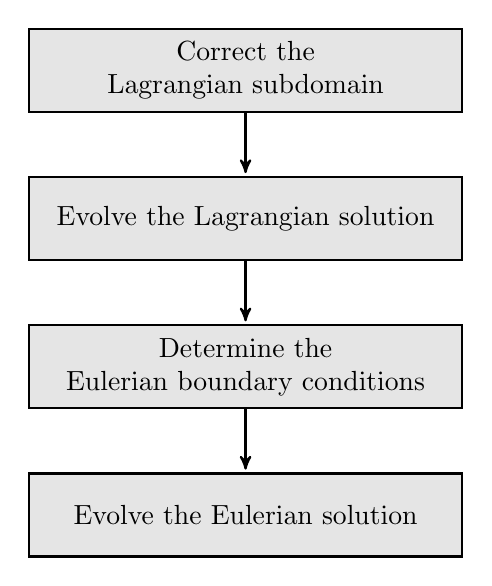
\begin{tikzpicture}
			[node distance=.8cm, start chain=going below,]
			\node[punktchain, join] (correct) {Correct the \\Lagrangian subdomain};
		    \node[punktchain, join] (evolveL) {Evolve the Lagrangian solution};
		    \node[punktchain, join] (bcE)     {Determine the \\Eulerian boundary conditions};
		    \node[punktchain, join] (evolveE) {Evolve the Eulerian solution};
		\end{tikzpicture}
		\caption{Flowchart of the simple coupling strategy. The flowchart shows the procedure to evolve both methods from $t_n$ to $t_{n+1}$.}
		\label{fig:flowchart_simpleCoupling}
	\end{figure}




% Summarize daenincks approach:
	% Methodology, algorithm
	% Domain decomposition
% Summarize stock's approach:
	% Methodology, algorithms
	% Resulted domain decomposition.
   	
   	\chapter{Implementation of Hybrid Eulerian-Lagrangian Vortex Particle Method}

   	% Chapter 5: Validation of Hybrid Method
	\chapter{Verification and Validation of Hybrid Method}
\label{ch:vavohm}

The verification and validation of the hybrid method focuses on 4 aspects:
\begin{itemize}
\item Lamb-Oseen vortex evolution at $Re=1000$(section \ref{sec:vvhm-love})
\item Clercx-Bruneau dipole convection at $Re=625$ (section \ref{sec:vvhm-cbdc})
\item Clercx-Bruneau dipole collision at $Re=550$ (section \ref{sec:vvhm-cbdcoll})
\item Stalled elliptical airfoil at $Re=5000$ (section \ref{sec:vvhm-ea})
\item Multi-body problem at $Re=550$ (section \ref{sec:vvhm-mb})
\end{itemize}

This chapter focuses on the verification and the validation of the hybrid method. We investigated several test-cases: the Lamb-Oseen vortex problem, the Clercx-Bruneau dipole collision by Clercx and Bruneau \cite{Clercx2006a}, the impulsively started cylinder test case, an elliptical airfoil at $Re=5000$ and a multi-body problem.

The implementation of the hybrid method was verified using the analytical solutions of the Lamb-Oseen vortex problem. The analytical solution of the problem enabled us to quantify the error in the scheme.

The validation of the hybrid solver was performed using the test cases provided from literature. The Clercx-Bruneau dipole collision problem of Clercx and Bruneau \cite{Clercx2006a}, provide a detailed analysis on the evolution of the vorticity field and the generation of vorticity from the boundary. The impulsively started cylinder problem investigated by Koumoutsakos and Leonard \cite{Koumoutsakos1995a}, and RosenFeld et al. \cite{MosheRosenFeldDochanKwak1991} showed the evolution of the forces acting on an immersed cylinder in a free-stream flow.

With a proper verification and validation of the hybrid solver, we were able to perform simulation of more complex problems. We were able to perform simulation of a stalled flow past a thin airfoil using an elliptical airfoil at $Re=5000$. Furthermore, a simulation of two cylinder in tandem showed the feasibility of simulation a multi-body problem. Both these simulations served as a proof of concept for a simulation of a full VAWT in future research.

\section{Lamb-Oseen Vortex Evolution}
\label{sec:vvhm-love}
The Lamb-Oseen vortex test case simulates the evolution of a laminar vortex core in an unbounded domain. In section \ref{subsec:lagrangianLambOseen}, we used this test case to verify and validate the implementation of the vortex blobs of the Lagrangian solver and in section \ref{subsec:eulerianLambOseen}, we used it to verify the implementation of the Eulerian solver. Therefore, in a similar fashion we employed this test case to verify the coupling of the hybrid solver. 

The unbounded nature of the problem helps us to neglect the influence of the solid boundary (i.e the wall). Therefore, this test case did not require the panel solver in the Lagrangian solver as we are only concerned with the coupling of the vortex blobs to the Eulerian solver. Thus, we primarily focused on the vorticity field interpolation error discussed in section \ref{subsubsec:vfie}. Furthermore, with the analytical solution, we were able to quantitatively present the importance of ensuring conservation of circulation.

Moreover, we were able to quantify the influences of the discretization on the accuracy of the coupling. A parameter sensitivity analysis was therefore performed to determine their effects on the coupling error. The parameters that determine the spatial discretization of the vortex blobs are the nominal particle spacing $h$, and the overlap ratio $\lambda$ (see figure \ref{fig:blobOverlap}). The spatial discretization of the Eulerian solver is regarded as a control variable for this test case as its impact was concluded in section \ref{subsec:eulerianLambOseen}. The parameters that determine the temporal discretization of the hybrid method are the time step size of the Eulerian solver $\Delta t_E$, and the time step size of the Lagrangian solver $\Delta t_L$. These are depended according to equation \ref{eq:timeStepDependency}, with $k_E$ being the number of Eulerian sub-steps.

The coupling error was quantified my determining the growth of maximum relative error in vorticity $\epsilon_{\omega}$ given by equation \ref{eq:maxRelErrorDef}, the approach used in section \ref{subsec:lagrangianLambOseen} and in section \ref{subsec:eulerianLambOseen}. 


\subsection{Problem Definition}

The Lamb-Oseen Vortex problem is defined by the vorticity field and the velocity field, equations \ref{eq:lo_voeq} and \ref{eq:lo_veeq}, respectively. The hybrid solver is initialized by first assigning the strengths of the vortex blobs using equation \ref{eq:lo_pie}. The Eulerian domain $\Omega_E$ is then initialized using the solution of the Lagrangian solver. Daeninck \cite{Daeninck2006} used this approach to enhance the coupling between the methods ensuring minimum interpolation error.

Figure \ref{fig:HLO_dc} shows the hybrid domain configuration for the Lamb-Oseen vortex problem with the Lagrangian domain $\Omega_L$ spanning the full fluid domain. The Eulerian domain $\Omega_E$ only resolves the center of the Lamb-Oseen core, $\Omega_E \subseteq \Omega_L$, bounding $[-0.5,-0.5] \times [-0.5,-0.5]$. The boundary of the Eulerian domain $\partial \Omega_E$ is a Dirichlet velocity boundary $\partial \Omega_E = [\Sigma_d]$ where the velocity boundary condition is applied, as described in section \ref{subsec:dbc}. The correction of the Lagrangian domain is performed in the interpolation domain $\Omega_{int}$ according to the procedures described in section \ref{sec:correction}.The boundary of the interpolation domain $\Sigma_{int}$ is defined with an offset $d_{bdry}$ from the Eulerian boundary $\Sigma_d$ by a distance $d_{bdry} = 2\cdot h$, where $h$ is the nominal blob spacing. Similar choice was made by Stock \cite{Stock2010a}, and ensures that the potential inaccuracies at the outer Eulerian boundary is ignored during the interpolation procedure.  

	\begin{figure}[!t]
	\showthe\columnwidth
	\centering
	\includegraphics[width=0.5\linewidth]{./figures/hybrid/lambOseen/hlo_dd-crop.pdf}
	\caption{(\emph{Not to scale}) The domain decomposition for the Lamb-Oseen vortex problem, $\Omega_E \subseteq \Omega_L$. The Eulerian domain is defined as $\Omega_E = [-0.5,0.5]\times[-0.5,0.5]$ with Dirichlet boundary $\partial \Omega_{dirichlet}$ [{\color{plotRed}{---}}, solid red]. The parameters of the discretization are tabulated in table \ref{tab:HLO_pt}.}
	\label{fig:HLO_dc}
	\end{figure}

The spatial discretization of the Eulerian domain $\Omega_E$ is regarded as a control (i.e fixed) variable. Therefore, the parameter sensitivity analysis is performed by varying the discretization of the Lagrangian method only. The Eulerian domain is discretized with an unstructured mesh formulation using GMSH (see section \ref{subsec:mgugmsh}) having $N_{cells} = 26448$ unstructured cells and grid size $h_{grid}$ ranging from $0.007$ to $0.0016$. 

The Lamb-Oseen vortex problem is defined according to the parameters tabulated in table \ref{tab:HLO_pt}. The center of the core is located at $(x,y)=(0,0)$, where the Eulerian domain $\Omega_E$ is also centered. The parameters are chosen such that vorticity $\omega$ and velocity $\mathbf{u}$ is non-zero at the boundary of the Eulerian domain $\Sigma_d$, figure \ref{fig:HLO_dc}. With the Lamb-Oseen time constant $\tau = 100$, this can be ensured.

The evolution of the Lagrangian solver and the Eulerian solver is performed according to sections \ref{sec:evolveLagrangian} and \ref{sec:evolveEulerian} respectively. The Lagrangian solver performs TRS for diffusion of the vortex blobs, see section \ref{subsubsec:srs}. The scheme requires vortex blob redistribution at every step, $f_{redis} = 1$. In conjunction with the redistribution, the population control is also performed at every step, $f_{pc}=1$ with $(\Gamma_{loc},\Gamma_{glob})$ as tabulated in table \ref{tab:HLO_pt}.

\subsection{Results and Discussion}

The investigation of the Lamb-Oseen vortex problem is divided into three parts. The first part of the investigation concerns with comparing several stages of the hybrid coupling, defined in section \ref{subsec:UvOvF}. We compared the uncoupled scheme with the one-way coupled scheme and with the fully coupled scheme. These successive coupling investigation helped us determine the source of the error, and furthermore quantify the errors in the coupling process. The second part of the investigation, section \ref{subsubsec:coc} focuses on importance of conservation of circulation that was discussed in section \ref{subsubsec:cc}. The results of the non-conserved and conserved scheme are compared to conclude the importance of conservation of circulation. During these two investigations, the parameters tabulated in table \ref{tab:HLO_pt} are used.

The third and final investigation is dedicated to the parameter sensitivity analysis, section \ref{subsubsec:psa}. The parameters that determine the spatial and temporal discretization of the scheme is investigated to verify the convergence of scheme.

	\ctable[
		caption = {Summary of the parameters for the Lamb-Oseen vortex evolution.},
		label   = {tab:HLO_pt},
		pos = !t,]{lcll}{}{\FL
		
		Parameters 					& Value 	& Unit					& Description \ML
		$\Gamma_c$\T               	& 1 &\si{m^2.s^{-1}} 				& Core strength\\
		$\Omega$               		& $[-0.5,0.5]\times[-0.5,0.5]$ &\si{m}		& Eulerian domain bounds \\
		$\nu$						& $0.001$ &\si{kg.s^{-1}.m^{-1}}& Kinematic viscosity\\
		$ \tau$ 		    		& $100$ 	&\si{s}	& Lamb-Oseen time constant\\
		$\lambda$						& 1 & - & Overlap ratio\\
		$h$							& 0.01 & \si{m} & Nominal blob spacing\\
		$(\Gamma_{loc},\Gamma_{glob})$			& (\num{1e-14}, \num{1e-14}) & - & Population control threshold\\
		$h_{grid}$ 					& \numrange{0.007}{0.016} & \si{m} & FE cell diameter span \\
		$ N_{\mathrm{cells}}$ 		& $26448$ 	& -						& Number of mesh cells\\
		$\Delta t_L$				& 0.001 & \si{s} & Lagrangian time step size\\
		$\Delta t_E$				& 0.001 & \si{s} & Eulerian time step size\\		
		$k_E$						& 1 & - & Eulerian sub-steps\\
		$ N_{\mathrm{t-steps}}$ 	& 1000 & -				& Number of time integration steps\\
		$t$ 		    			& \numrange{0}{1} 	&\si{s}			& Simulation time span\\		
		$d_{bdry}$					& $2\cdot{h}$ & \si{m} & Interpolation boundary offset\LL}

\subsubsection{Uncoupled vs. One-way Coupled vs. Fully Coupled}
\label{subsec:UvOvF}
The several stages of the hybrid coupling with the fully Eulerian test case, to verify the implementation of the hybrid algorithm. The three stages of the coupling are as follows:

\begin{itemize}
\item \textbf{Uncoupled}: The uncoupled test case involves only the Eulerian solver and serves as a benchmark to quantify the error in the coupling. The boundary conditions are determined directly from the analytical formulation, equation \ref{eq:eLO_veq}.
\item \textbf{One-way coupled}: The one-way coupled test case is a partially coupled hybrid test case where the Eulerian method is evolved using the Lagrangian solution. The correction of the Lagrangian solution is not performed in this scenario. Thus, this case helped us determine the error in the evolution of the Eulerian method using the Lagrangian solution.
\item \textbf{Fully coupled}: The fully coupled test case performs the full coupling strategy described in section \ref{subsec:mcs}. The Eulerian method is evolved using the Lagrangian solution. At the end of each time step, the Lagrangian solution inside the interpolation domain $\Omega_{int}$, figure \ref{fig:HLO_dc}, is corrected. This test case helped us quantify the error in transferring the Eulerian solution to the Lagrangian method.
\end{itemize}
	
	\begin{figure}[h]
     \centering
     \begin{subfigure}[t]{0.45\textwidth}
             \includegraphics[width=\linewidth]{./figures/hybrid/lambOseen/lambOseen_fully_vErrorInitial_raster.png}
             \caption{Velocity}
             \label{fig:lambOseen_oneway_vErrorInitial}
     \end{subfigure}%
     \qquad %add desired spacing between images, e. g. ~, \quad, \qquad etc.
       %(or a blank line to force the subfigure onto a new line)
     \begin{subfigure}[t]{0.45\textwidth}
             \includegraphics[width=\linewidth]{./figures/hybrid/lambOseen/lambOseen_fully_wErrorInitial_compressed.png}
             \caption{Vorticity}
             \label{fig:lambOseen_uncoupled_wErrorInitial}
     \end{subfigure}
     \caption{Initial relative error at $t=0$ inside the Eulerian domain $\Omega_E$. The figure depicts \textbf{(a)} the relative error in velocity $\mathbf{u}$, and \textbf{(b)} the relative error in vorticity $\omega$.}
     \label{fig:lambOseen_initialError}
	\end{figure}
		
Figure \ref{fig:lambOseen_initialError} depicts the initial relative error in velocity and vorticity inside the Eulerian domain $\Omega_E$. The relative error in velocity is near machine epsilon $\epsilon \le \num{e-10}$, but the error in vorticity is in the order of \num{e-5}. A similar observation was made in section \ref{subsec:eulerianLambOseen}, and it concluded that the source of the error is the projection error of the finite element when determining the vorticity $\omega$ from velocity $\mathbf{u}$, described in section \ref{subsec:dtvf}. 

	\begin{figure}[!b]
	\centering
	\includegraphics[width=0.6\linewidth]{./figures/hybrid/lambOseen/lambOseen_comparision_compressed.pdf}
	\caption{Evolution of the maximum relative error in velocity (dashed) and the maximum relative error in vorticity (solid), equation \ref{eq:maxRelErrorDef}, from $t=0$ to $t=1$, using the parameters tabulated in table \ref{tab:HLO_pt}. The figure compares uncoupled case (\textbf{black}) vs. the one-way coupled case ({\color{plotBlue}{\textbf{blue}}}) vs. the fully coupled case ({\color{plotRed}{\textbf{red}}}).}
	\label{fig:lambOseen_comparison}
	\end{figure}

The simulation was evolved from $t=0$ to $t=1$ with $N_{t-steps} = 1000$ Lagrangian time steps with $k_E=1$ Eulerian sub-steps. A detailed summary of the time step parameters is tabulated in table \ref{tab:HLO_pt}. Figure \ref{fig:lambOseen_comparison} shows the evolution of maximum relative error in vorticity $\omega$ and velocity $\mathbf{u}$ of the uncoupled, one-way coupled and the fully coupled cases inside the Eulerian domain $\Omega_E$ w.r.t. the analytical solution, equation \ref{eq:lo_voeq}. The initial observation shows that the error in velocity is two to three orders of magnitude lower than the error in vorticity (due to the projection error). The figure shows that the uncoupled scheme has the lowest error in vorticity and velocity. As the boundary condition is directly obtained from the analytical solution, the error only arises from the FE discretization of the Eulerian method. As the time progresses, the error in velocity converges near \num{e-7} and the error in vorticity converges near \num{e-4}.

	\begin{figure}[!b]
     \centering
     \begin{subfigure}[t]{0.45\textwidth}
             \includegraphics[width=\linewidth]{./figures/hybrid/lambOseent2/lambOseen_uncoupled_vErrorFinal_compressed-crop.png}
             \caption{Uncoupled; velocity $\mathbf{u}$}
             \label{fig:lambOseen_uncoupled_vErrorFinal}
     \end{subfigure}%
     \qquad %add desired spacing between images, e. g. ~, \quad, \qquad etc.
       %(or a blank line to force the subfigure onto a new line)
     \begin{subfigure}[t]{0.45\textwidth}
             \includegraphics[width=\linewidth]{./figures/hybrid/lambOseent2/lambOseen_uncoupled_wErrorFinal_compressed-crop.png}
             \caption{Uncoupled; vorticity $\omega$}
             \label{fig:lambOseen_uncoupled_wErrorFinal}
     \end{subfigure}%       
       
     \begin{subfigure}[t]{0.45\textwidth}
             \includegraphics[width=\linewidth]{./figures/hybrid/lambOseent2/lambOseen_oneway_vErrorFinal_compressed-crop.png}
             \caption{One-way coupled; velocity $\mathbf{u}$}
             \label{fig:lambOseen_oneway_vErrorFinal}
     \end{subfigure}
     \qquad
     \begin{subfigure}[t]{0.45\textwidth}
             \includegraphics[width=\linewidth]{./figures/hybrid/lambOseent2/lambOseen_oneway_wErrorFinal_compressed-crop.png}
             \caption{One-way coupled; vorticity $\omega$}
             \label{fig:lambOseen_oneway_wErrorFinal}
     \end{subfigure}     
   
     \begin{subfigure}[t]{0.45\textwidth}
             \includegraphics[width=\linewidth]{./figures/hybrid/lambOseent2/lambOseen_fully_vErrorFinal_compressed-crop.png}
             \caption{Fully coupled; velocity $\mathbf{u}$}
             \label{fig:lambOseen_fully_vErrorFinal}
     \end{subfigure}     
     \qquad
     \begin{subfigure}[t]{0.45\textwidth}
             \includegraphics[width=\linewidth]{./figures/hybrid/lambOseent2/lambOseen_fully_wErrorFinal_compressed-crop.png}
             \caption{Fully coupled; vorticity $\omega$}
             \label{fig:lambOseen_fully_wErrorFinal}
     \end{subfigure}        
     
     \caption{Plot of the relative error in velocity (\textit{left}) and relative error in vorticity (\textit{right}) in the Eulerian domain $\Omega_E$ at $t=1$. The figure compares the error between \textbf{(a)}\textbf{(b)} the uncoupled, \textbf{(c)}\textbf{(d)} the one-way coupled, and \textbf{(e)}\textbf{(f)} the fully coupled cases.}
     \label{fig:lambOseen_finalError}
	\end{figure}

The one-way coupled case shows an increase in the relative error in velocity field $\mathbf{u}$ inside the Eulerian domain $\Omega_E$. However, the difference is negligible at the initial stages of the simulation. This states that the analytical solution was well represented by the vortex blobs with a small discretization error. However by $t=1$, the error in velocity increases by two orders of magnitude from \num{e-7} to \num{e-5}, w.r.t to the uncoupled scheme. This implies that the source of the error is due to the time integration error of the Lagrangian method. In section \ref{subsec:lagrangianLambOseen}, we observed similar trend of growth in error due to time-marching of the vortex blobs.

The fully coupled case demonstrates that there is an additional increase in the error. Unlike the one-way coupled case, the increase in the error is observed from the start of the simulation, implying that the increase in the error is due to the correction of the strengths of the vortex blobs. In section \ref{subsec:hy_iwtca}, we discussed that the re-initialization of the vortex blobs introduces smoothing error in the vorticity field (i.e the Gaussian blurring of the vorticity field). This causes the Lagrangian solution to further deviate from the analytical solution of the Lamb-Oseen vortex. The consequence of this was that at $t=1$, the error in vorticity $\epsilon_{\omega}$ increased from \num{e-4} to \num{e-3} and the error in velocity increased from \num{e-5} to \num{e-4}, w.r.t the one-way coupled case.
%The transfer of the discrete vorticity field from the Eulerian method to the Lagrangian method (i.e the correction process) causes an additional increase in the discretization error of the Lagrangian solution. This causes the Lagrangian solution to further deviate from the analytical solution of the Lamb-Oseen vortex. The main component of the discretization error is the smoothing error (i.e Gaussian blurring of the vorticity field) when using mollified vortex kernels, discussed in section \ref{subsec:hy_iwtca}. The Gaussian blurring of the vorticity field adds an additional error when re-initializing the vortex blobs inside the interpolation domain $\Omega_{int}$.		

Figure \ref{fig:lambOseen_finalError} shows the relative error in velocity and vorticity inside the Eulerian domain $\Omega_E$ at $t=1$, for the three stages of coupling. We observe that there is an increase in error when going from the uncoupled scheme to the one-way coupled scheme to the fully coupled. Comparing the uncoupled scheme to the one-way coupled scheme, an increase in error is observed at the boundary of the Eulerian domain $\Sigma_d$.  Comparing the one-way coupled to fully coupled case, we see that there is an additional increase in the error from the boundary. Therefore, the artificial vorticity generated from the boundary is due to the mismatch in the solutions of the Eulerian and the Lagrangian method. A larger mismatch in the solution will introduce strong artificial vorticity from the boundary.
%The error originates from the small error in the Dirichlet boundary conditions at the boundary $\Sigma_d$. due to the larger error in the Dirichlet boundary condition. Figure \ref{fig:lambOseen_fully_wErrorFinal} clearly shows this artificial vorticity generated from the boundary, and can be concluded that this is due to the mismatch in the solutions of the Eulerian and the Lagrangian method.

The strength of the artificial vorticity at the boundary is proportional to the error in the coupling and to ensure an accurate coupling scheme, we have ensure this vorticity does not corrupt the characteristics of the original vorticity field. Therefore, we modified the discretization of the Lagrangian field such that the artificial vorticity generated from the boundary is less the threshold of influence (i.e $<1\%$ of the maximum vorticity $\max\{\omega\}$).

\subsubsection{Conservation of circulation}
\label{subsubsec:coc}

The approach for ensuring conservation of circulation during the coupling process was discussed in section \ref{subsubsec:cc}. To validate the importance of conservation of circulation, we ran two simulation with and without the conservation of circulation during the transfer of vorticity from the Eulerian method to the Lagrangian method. The control variables of the simulation are the parameters tabulated in table \ref{tab:HLO_pt}.

Figure \ref{fig:lambOseen_conservation_contourf} compares the error in the Eulerian domain $\Omega_E$ of the coupling approach without the conservation circulation against the approach satisfying the conservation of circulation, at $t=1$. We see that the scheme without the conservation has significantly larger error than the scheme with conservation. The maximum error is near the Eulerian boundary $\Sigma_d$ and shows an increase in the artificial vorticity emanating from the boundary due to the larger mismatch in the solutions, figure \ref{fig:lambOseen_fullyCoff_wErrorFinal}. However, when we ensure that circulation is conserved, figure \ref{fig:lambOseen_fullyCon_wErrorFinal}, the boundary produces significantly less error.

	\begin{figure}[!t]
     \centering
     \begin{subfigure}[t]{0.45\textwidth}
             \includegraphics[width=\linewidth]{./figures/hybrid/lambOseent2/lambOseen_fully_vErrorFinal_compressed-crop.png}
             \caption{Conservation \texttt{on}; velocity $\mathbf{u}$}
             \label{fig:lambOseen_fullyCon_vErrorFinal}
     \end{subfigure}%
     \qquad %add desired spacing between images, e. g. ~, \quad, \qquad etc.
       %(or a blank line to force the subfigure onto a new line)
    \begin{subfigure}[t]{0.45\textwidth}
             \includegraphics[width=\linewidth]{./figures/hybrid/lambOseent2/lambOseen_fully_wErrorFinal_compressed-crop.png}
             \caption{Conservation \texttt{on}; vorticity $\omega$}
             \label{fig:lambOseen_fullyCon_wErrorFinal}
     \end{subfigure}%     
            
     \begin{subfigure}[t]{0.45\textwidth}
             \includegraphics[width=\linewidth]{./figures/hybrid/lambOseent2/lambOseen_fullyCoff_vErrorFinal_compressed-crop.png}
             \caption{Conservation \texttt{off}; velocity $\mathbf{u}$}
             \label{fig:lambOseen_fullyCoff_vErrorFinal}
     \end{subfigure}
     \qquad     
     \begin{subfigure}[t]{0.45\textwidth}
             \includegraphics[width=\linewidth]{./figures/hybrid/lambOseent2/lambOseen_fullyCoff_wErrorFinal_compressed-crop.png}
             \caption{Conservation \texttt{off}; vorticity $\omega$}
             \label{fig:lambOseen_fullyCoff_wErrorFinal}
     \end{subfigure}  
  
     \caption{Plot of the relative error in velocity (left) and the relative error in vorticity (right) in the Eulerian domain $\Omega_E$ at $t=1$. The figure compares the error between \textbf{(a)}\textbf{(b)} without conservation of circulation, and \textbf{(c)}\textbf{(d)} with the conservation of circulation.}
     \label{fig:lambOseen_conservation_contourf}
	\end{figure}
	
	\begin{figure}[!p]
	\centering
	\includegraphics[width=0.6\linewidth]{./figures/hybrid/lambOseent2/lambOseen_comparision_conservation_compressed.pdf}
	\caption{Plot of the maximum relative error in vorticity $\epsilon_{\omega}$ [ - -, dashed] and maximum relative error in vorticity $\epsilon_{\mathbf{u}}$ [ ---, solid], equation \ref{eq:maxRelErrorDef}, from $t=0$ to $t=1$, using the parameters tabulated in table \ref{tab:HLO_pt}. The figure compares the coupling scheme with conservation of circulation ({\color{plotRed}{\textbf{red}}}) vs. the coupling scheme without conservation of circulation ({\color{plotGreen}{\textbf{green}}}).}
	\label{fig:lambOseen_comparision_conservation}
	\end{figure}	

	\begin{figure}[!p]
	\centering
	\includegraphics[width=0.6\linewidth]{./figures/hybrid/lambOseent2/lambOseen_comparision_conservation_circulation_compressed.pdf}
	\caption{Plot of the error in total circulation $\epsilon_{\Gamma}$ of the Lagrangian method from $t=0$ to $t=1$. The figure compares the scheme with conservation of circulation [ {\color{plotRed}{\textbf{---}}}, solid {\color{plotRed}{\textbf{red}}}], and the scheme without conservation of circulation [ {\color{plotGreen}{\textbf{---}}}, solid {\color{plotGreen}{\textbf{green}}}].}
	\label{fig:lambOseen_comparision_conservation_circulation}
	\end{figure}	

Figure \ref{fig:lambOseen_comparision_conservation} shows the evolution of the maximum relative error from $t=0$ to $t=1$, comparing the results of with and without the conservation of circulation. Observing the difference in the relative error in velocity and vorticity, we see that the scheme without the conservation of circulation produces larger error at all times $t$. At $t=1$, we observe that scheme without the conservation of circulation has a relative error in vorticity near \num{e-2}, whereas with the conservation of circulation, the relative error is an order of magnitude lower, reaching only \num{e-3}. Similarly for velocity, the scheme without the conservation of circulation has the relative error approaching \num{e-3}, whereas with the conservation enabled, the error only reaches \num{e-4}. 

Figure \ref{fig:lambOseen_comparision_conservation_circulation} shows the change in total circulation from $t=0$ to $t=1$ for the non-conserved and conserved scheme. It is apparent that without the conservation of circulation, the error in total circulation is significantly larger and approaches \num{e-3}. If the circulation is not conserved explicitly, the transfer of vorticity from the Eulerian method to the Lagrangian method introduces additional error in total circulation. By ensuring conservation of circulation, as described in section \ref{subsubsec:cc}, we see that the error in total circulation is significantly smaller, near \num{e-10}. %It is to be noted that there will be still a linear increase in the total circulation is due to the population control of the vortex blobs, removing the circulation $\Gamma_{glob}$ at every evaluation, as described in section \ref{subsubsec:srs}.

In summary, we have determined that to ensure minimum error during the transfer of Eulerian solution to the Lagrangian solution, we have to ensure that the total circulation of the Lagrangian method is conserved.

\subsubsection{Parameter sensitivity analysis}
\label{subsubsec:psa}

The parameter sensitivity analysis is the last stage of the Lamb-Oseen vortex investigation. The Lamb-Oseen vortex test case was ideal to determining the effects of the temporal and the spatial discretization of the hybrid method on the accuracy of the coupling. 

To investigate the effects of the spatial discretization on the accuracy of the coupling, we ran several test cases varying the nominal blob spacing $h$, and test cases varying the overlap ratio $\lambda$. To investigate the effects of temporal discretization, we modified the Lagrangian time step size $\Delta t_L$ w.r.t the Eulerian time step size $\Delta t_E$. The control variables of the simulations are the ones tabulated in table \ref{tab:HLO_pt}.

	\begin{figure}[!b]
	\centering
	\includegraphics[width=0.6\linewidth]{./figures/hybrid/lambOseen/lambOseen_parameter_h.pdf}
	\caption{Evolution of the maximum relative error for various nominal blob spacing $h = [0.01,0.02,0.05,0.1]$ from $t=0$ to $t=1$. The figures shows the maximum relative error in vorticity [ - -, dashed] and maximum relative error in vorticity [ ---, solid].}
	\label{fig:lambOseen_parameter_h}
	\end{figure}	
	
Figure \ref{fig:lambOseen_parameter_h} shows the impact of varying the nominal blob spacing $h$ on the coupling. The maximum relative error in vorticity and the maximum relative error in velocity is plotted from $t=0$ to $t=1$ for nominal blob spacing $h = [0.01,0.02,0.05,0.1]$. The figure shows that increasing the spatial resolution of the Lagrangian method reduces the error. At $t=1$, the minimum error is observed for $h=0.01$ with the relative error in velocity at \num{e-4} and the relative error in vorticity at \num{e-3}. The maximum relative error is observed for $h=0.1$, with \num{e-3} for relative error in velocity and \num{e-2} for relative error in vorticity. This implies that the growth in error is of order one. Figure \ref{fig:lambOseen_parameter_h_Trend} shows the variation in the maximum relative error in vorticity at $t=1$ for various nominal blob spacing $h$. The figure indeed shows that the change in error due to the spatial discretization is of order one.

	\begin{figure}[!p]
	\centering
	\includegraphics[width=0.6\linewidth]{./figures/hybrid/lambOseen/lambOseen_parameter_h_Trend.pdf}
	\caption{Convergence of the maximum relative error in vorticity due to the nominal blob spacing $h = [0.01,0.02,0.05,0.1]$.}
	\label{fig:lambOseen_parameter_h_Trend}
	\end{figure}
	
	\begin{figure}[!p]
	\centering
	\includegraphics[width=0.6\linewidth]{./figures/hybrid/lambOseen/lambOseen_parameter_overlap.pdf}
	\caption{Evolution of the maximum relative error for various overlap ratios $\lambda = [0.5, 0.75, 1.0, 1.5]$ from $t=0$ to $t=1$. The figures shows the maximum relative error in vorticity [ - -, dashed] and the maximum relative error in vorticity [ ---, solid].}
	\label{fig:lambOseen_parameter_overlap}
	\end{figure}		

	\begin{figure}[!p]
     \centering
     \begin{subfigure}[t]{0.45\textwidth}
             \includegraphics[width=\linewidth]{./figures/hybrid/lambOseen/lambOseen_parameter_k.pdf}
             \caption{$\Delta t_L = [0.001,0.002,0.005,0.01]$, $\Delta t_E = 0.001$}
             \label{fig:lambOseen_parameter_k_dtL}
     \end{subfigure}     
     \qquad
     \begin{subfigure}[t]{0.45\textwidth}
             \includegraphics[width=\linewidth]{./figures/hybrid/lambOseen/lambOseen_parameter_k_dtE.pdf}
             \caption{$\Delta t_E = [0.001,0.0005,0.0002]$, $\Delta t_L = 0.001$}
             \label{fig:lambOseen_parameter_k_dtE}
     \end{subfigure}        
     
     \caption{Evolution of the maximum relative error from $t=0$ to $t=1$ for various number of Eulerian sub-steps $k_E = [1,2,5,10]$, modifying (\textbf{a}) the Lagrangian time step $\Delta t_L$, and (\textbf{b}) the Eulerian time step $\Delta t_E$. The figures shows the maximum relative error in vorticity [ - -, dashed] and maximum relative error in vorticity [ ---, solid].}
     \label{fig:lambOseen_parameter_k}
	\end{figure}	


Figure \ref{fig:lambOseen_parameter_overlap} compares the evolution of the maximum relative error for various overlap ratios, $\lambda = [0.5, 0.75, 1.0, 1.5]$. We see that the minimum error in velocity and vorticity is observed for the overlap ratio $\lambda = 1$. As we move from this value, an increase in the error is observable. In section \ref{subsubsec:convergenceInterpolation}, we determined that to reduce the Gaussian blurring of the vorticity field from the Gaussian vortex kernels, we require an overlap ratio $\lambda=1$ and a small nominal blob spacing $h$. The parameter sensitivity analysis on the spatial discretization validates this observation and states that to ensure minimum error in coupling, these criteria has to be satisfied.

Figure \ref{fig:lambOseen_parameter_k} shows the impact of varying the temporal discretization of the Lagrangian method and the Eulerian method w.r.t each other. The relation of the Eulerian time step size $\Delta t_E$ to the Lagrangian time step size $\Delta t_L$ is described in section \ref{subsec:mse}. Figure \ref{fig:lambOseen_parameter_k_dtL} shows the effect of modifying the Lagrangian time step size $\Delta t_L$ w.r.t to a fixed Eulerian time step size. With $\Delta t_E=0.001$ and the number of Eulerian sub-steps $k_E = [1,2,5,10]$, we have $\Delta t_L = k_E\cdot\Delta t_E = [0.001,0.002,0.005,0.01]$.Similarly, figure \ref{fig:lambOseen_parameter_k_dtE} shows the effect of modifying the Eulerian time step size $\Delta t_E$ w.r.t to the Lagrangian time step. With $\Delta t_L=0.001$ and $k_E = [1,2,5]$, we have $\Delta t_E = \Delta t_L/k_E = [0.001,0.0005,0.0002]$. We see that the minimum error occurs when the time steps match (i.e $\Delta t_L = \Delta t_E$). However if increase the number of Eulerian time steps from $k_E = 1 $ to $k_E=2$, there an substantial increase in the relative error in velocity. This observation states that the linear interpolation used for sub-stepping process, has potential for improvement. A possible solution might be to employ a higher-order interpolation method for determining the Eulerian Dirichlet boundary condition at the sub-steps.

%Figure \ref{fig:lambOseen_parameter_k_Trend} shows the convergence trend of error in vorticity due to number of Eulerian sub-step $k_E$. 
%
%	\begin{figure}[!h]
%	\centering
%	\includegraphics[width=0.6\linewidth]{./figures/hybrid/lambOseen/lambOseen_parameter_h_Trend.pdf}
%	\caption{Convergence of the error in coupling due to the number of Eulerian sub-step $k_E$ at $t=1$. The control variables are tabulated in table \ref{tab:HLO_pt}}.
%	\label{fig:lambOseen_parameter_k_Trend}
%	\end{figure}

\subsection{Conclusion}

In section \ref{subsec:UvOvF}, we observed that moving from uncoupled to one-way coupled case, increases the relative error in velocity. The growth in error was mainly due to the time integration error of the Lagrangian method. When moving from one-way coupled to fully coupled scheme, there is a tangible increase in the relative error in vorticity and an additional increase in the error in velocity. The increase in this error was due to the re-initialization of the vortex blobs introducing an additional smoothing error at each correction step.

In section \ref{subsubsec:coc}, we observed that conservation of circulation is vital in ensuring an accurate coupling strategy. The transfer of vorticity from the Eulerian method to the Lagrangian method, must be performed with a focus on the conservation of circulation, to ensure that the artificial vorticity at the Eulerian Dirichlet boundary $\Sigma_d$ is minimal.

In section \ref{subsubsec:psa}, we investigated the impact of varying the spatial and temporal discretization on the accuracy of the coupling. We determined there is an increase in error, if the Lagrangian method is spatially under-resolved w.r.t to the Eulerian method. An overlap ratio of $\lambda=1$ was shown to have the minimum error during the coupling, as it ensures minimum Gaussian blurring. Varying the number of Eulerian sub-steps $k_E$, showed that the linear interpolation for the Dirichlet boundary condition is potential source of improvement.

\section{Clercx-Bruneau Dipole Convection}
\label{sec:vvhm-cbdc}

In section \ref{sec:vvhm-love}, we determine the effects of transferring the Lagrangian solution to the Eulerian method, and transferring the Eulerian solution back to the Lagrangian method on an Lamb-Oseen vortex test case. However, an important aspect of domain decomposition method is the entering and the exiting of a vortex core in the Eulerian domain $\Omega_E$. We used the Clercx-Bruneau dipole \cite{Clercx2006a} to simulate the convection of vortex an Eulerian domain $\Omega_E$. 

\subsection{Problem Definition}

The hybrid domain decomposition of this investigation is depicted in figure \ref{fig:hcbconv_dd}. The Eulerian domain $\Omega_E$ is finite with bounds $[-0.25,0.25]\times[-0.5,0.5]$. The Clercx-Bruneau dipole, defined by equation \ref{fig:hcbconv_dd}, is initialized outside the Eulerian domain $\Omega_L\backslash\Omega_E$ at $(x_1,y_1) = (-1,0.1)$ and $(x_2,y_2)=(-1,-0.1)$, corresponding to the positive and negative cores, respectively. As the simulation progresses, the dipole convects along the $x$-axis, passing through the Eulerian domain.

	\begin{figure}[!h]
	\showthe\columnwidth
	\centering
	\includegraphics[trim=0cm 2.5cm 0cm 2.5cm, clip, width=\linewidth]{./figures/hybrid/cbConv/hcbconv_dd.pdf}
	\caption{(\textit{Not to Scale}) The domain decomposition for the Clercx-Bruneau convection problem, with the positive pole located at $p_{+}=(x_1,y_1) = (-1,0.1)$ and negative pole located at $p_{-}=(x_2,y_2)=(-1,-0.1)$. The parameters of the simulation are tabulated in table \ref{tab:HcbConvection_pt}.}
	\label{fig:hcbconv_dd}
	\end{figure}
	
The Eulerian and the Lagrangian domain is discretized according to the parameters shown in table \ref{tab:HcbConvection_pt}. The focus of this simulation is the entry and the exit of vorticity from in and out of the Eulerian domain and its impact on the solution. The simulation was first benchmarked using a Finite Element (FE) only simulation, and a Vortex Particle Method (VPM) only simulation, providing an basis for hybrid simulation. We can assume that the FE and VPM simulation are valid as we have already verified and validated their implementation in section \ref{sec:volm} and \ref{sec:eu-voem}, respectively.

To ensure that FE only simulation was valid, the Eulerian domain $\Omega_E$ stretched up to the far-field of the dipole, where the vorticity and the induced velocity is zero. The Eulerian domain $\Omega_E$ of the FE only simulation spanned $[-3,3]\times[-2,2]$. For a valid comparison, these benchmark simulations followed similar parameters as the ones tabulated in table \ref{tab:HcbConvection_pt}.

	\ctable[
		caption = {Summary of the parameters for the Clercx-Bruneau dipole convection problem.},
		label   = {tab:HcbConvection_pt},
		pos = !t,]{lcll}{\tnote[a]{Obtained from Renac et al. \cite{Renac2013}}}{\FL
		
		Parameters 					& Value 	& Unit					& Description \ML
		$\Omega_E$             		& $[-0.25,0.25]\times[-0.5,0.5]$ &\si{m}	& Eulerian domain bounds \\
		$Re$						& 625 & - & Reynolds number\\
		$U$							& 1 & \si{m.s^{-1}} & Characteristic velocity\\
		$W$							& 1 & \si{m} & Characteristic Length\\
		$\nu$						& \num{1.6e-3} & \si{kg.s^{-1}.m^{-1}} & Kinematic viscosity\\
		$(x,y)_{1,2}$				& $(-1,\pm0.1)$ & \si{m} & Initial location of the monopoles\\
		$\omega_e$					& 299.528385375226\tmark[a] & - & Characteristic vorticity of the monopole\\
		$\lambda$					& 1 & - & Overlap ratio\\
		$h$							& 0.005 & \si{m} & Nominal blob spacing\\
		$h_{grid}$ 					& $\approx0.007$ & \si{m}	& FE cell diameter \\
		$ N_{\mathrm{cells}}$ 		& $40000$ 	& -						& Number of mesh cells\\
		$\Delta t_L$				& \num{2.5e-4} & \si{s} & Lagrangian time step size\\
		$\Delta t_E$				& \num{2.5e-5} & \si{s} & Eulerian time step size\\		
		$k_E$						& 10 & - & Eulerian sub-steps\\
		$ N_{\mathrm{t-steps}}$ 	& 2800 & -			& Number of time integration steps\\
		$t$							& 0 to 0.7 & - & Simulation time\\
		$d_{bdry}$					& $2\cdot{h}$ & \si{m} & Interpolation boundary offset\LL}


\subsection{Results and Discussion}

Figure \ref{fig:hybrid_doubleMonopoleConvection_contourfPlots} compares the vorticity field of the FE simulation and the hybrid simulation at various instances, $t=[0,0.2,0.4,0.6]$. The top half of each subplot belongs to the hybrid simulation, whereas the bottom half to the FE only simulation. It was determined that the cores of the dipole enters the Eulerian domain at $t=0.26$ and exits the domain at $t=0.45$. The figure shows that solution of both simulation matches up to the entry of the dipole, figure \ref{fig:hybrid_doubleMonopoleConvection_contourfPlots}a and figure \ref{fig:hybrid_doubleMonopoleConvection_contourfPlots}b. However in figure \ref{fig:hybrid_doubleMonopoleConvection_contourfPlots}c, the solutions start to deviate, and at $t=0.7$, figure \ref{fig:hybrid_doubleMonopoleConvection_contourfPlots}d, it is apparent that the dipole in the hybrid method is lagging w.r.t to the FE only simulation. This would imply that the passage of the vortex through the domain has a stalling influence on the vorticity evolution.

To investigate further on this influence of the passage, we analyzed variation in maximum vorticity $\omega_{max}$. Figure \ref{fig:hybrid_dipoleConvection_hybridSubDomains_wMax} shows evolution of the maximum vorticity $\omega_{max}$ from $t=0$ to $t=0.7$ in the Eulerian and the Lagrangian sub-domain of the hybrid simulation, the FE only simulation, and the VPM only simulation. We observe there is a slight difference in the maximum vorticity for the FE only and the VPM only simulation, which increases as the time progresses.

At $t=0.26$, the maximum vorticity in the Eulerian sub-domain starts to increase, signifying the entering of the vortex core. Similarly, at $t=0.45$, the maximum vorticity starts to decrease, signifying the exiting of the vortex core. As the dipole enters the sub-domain, there is slight drop in the maximum vorticity. Similarly, as the dipole exits, there a slight peak in the solution of the Eulerian sub-domain. The explanation to the increases in the vorticity in the Eulerian domain is the generation of the artificial vorticity. When the core of the dipole is right next the Eulerian boundary $\Sigma_d$, the influence of the vorticity on the boundary is larger. However, with the implementation of Stocks interpolation tolerance at the boundary, this artificial vorticity is somewhat neglected.
%A possible explanation to this phenomena might be error due to the artificial vorticity at the boundary. In section \ref{}, we observed that error in coupling introduces artificial vorticity at the boundary and the strength of this vorticity is proportional to the error in coupling. 
	
	\begin{figure}[!b]
	\showthe\columnwidth
	\centering
	\includegraphics[width=\linewidth]{./figures/hybrid/cbConv/hybrid_doubleMonopoleConvection_contourfPlots-crop.png}
	\caption{Plot of the Clercx-Bruneau dipole at $t=[0,0.2,0.4,0.7]$ using parameters tabulated in table \ref{tab:HcbConvection_pt}. The figure compares the hybrid simulation (top halves) against the FE only simulation (bottom halves).}
	\label{fig:hybrid_doubleMonopoleConvection_contourfPlots}
	\end{figure}

	\begin{figure}[!p]
     \centering
     \begin{subfigure}[t]{0.48\textwidth}
             \includegraphics[width=\linewidth]{./figures/hybrid/cbConv/hybrid_dipoleConvection_hybridSubDomains_wMax.pdf}
             \caption{Comparison of the hybrid sub-domains}
             \label{fig:hybrid_dipoleConvection_hybridSubDomains_wMax}
     \end{subfigure}     
     ~ %\qquad
     \begin{subfigure}[t]{0.48\textwidth}
             \includegraphics[width=\linewidth]{./figures/hybrid/cbConv/hybrid_dipoleConvection_comparison_parameter_wMax.pdf}
             \caption{Comparison with a less resolved hybrid method}
             \label{fig:hybrid_dipoleConvection_comparison_parameter_wMax}
     \end{subfigure}        
     
     \caption{Evolution of the maximum vorticity $\max\{\omega\}$ from $t=0$ to $t=0.7$. The solutions are compared with the benchmark results of FE only [---, solid black], and VPM only [- -, dashed black] simulations. The figure depicts (\textbf{a}) the maximum vorticity in the Eulerian and the Lagrangian sub-domain of the hybrid method, and (\textbf{b}) the maximum vorticity of hybrid method with nominal blob spacing $h=0.01$ and $h=0.005$.}
     \label{fig:hybrid_dipoleConvection_comparison_wMax}
	\end{figure}	
	
	\begin{figure}[!p]
     \centering
     \begin{subfigure}[t]{0.48\textwidth}
             \includegraphics[width=\linewidth]{./figures/hybrid/cbConv/hybrid_doubleMonopoleConvection_entering2.pdf}
             \caption{Entering at $t=0.26$}
             \label{fig:hybrid_doubleMonopoleConvection_entering2}
     \end{subfigure}     
     ~ %\qquad
     \begin{subfigure}[t]{0.48\textwidth}
             \includegraphics[width=\linewidth]{./figures/hybrid/cbConv/hybrid_doubleMonopoleConvection_exiting.pdf}
             \caption{Exiting at $t=0.45$}
             \label{fig:hybrid_doubleMonopoleConvection_exiting}
     \end{subfigure}        
     
     \caption{Vorticity contour plots of the dipole with levels ...,-50,-30,-10,10,30,50,... of the Eulerian and the Lagrangian sub-domains. The figure highlights the effect of the artificial vorticity at the boundary of the Eulerian domain.}
     \label{fig:hybrid_doubleMonopoleConvection_ent_exi}
	\end{figure}
	
	\begin{figure}[!p]
     \centering
     \begin{subfigure}[t]{0.48\textwidth}
             \includegraphics[width=\linewidth]{./figures/hybrid/cbConv/hybrid_dipoleConvection_comparison_parameter_E.pdf}
             \caption{Kinetic energy $E$}
             \label{fig:hybrid_dipoleConvection_comparison_parameter_E}
     \end{subfigure}     
     ~
     \begin{subfigure}[t]{0.48\textwidth}
             \includegraphics[width=\linewidth]{./figures/hybrid/cbConv/hybrid_dipoleConvection_comparison_parameter_Omega.pdf}
             \caption{Enstrophy $\Omega$}
             \label{fig:hybrid_dipoleConvection_comparison_parameter_Omega}
     \end{subfigure}        
     
     \caption{Evolution of the (\textbf{a}) kinetic energy $E$ and (\textbf{b}) enstrophy for the nominal blob spacing $h=0.01$ and $h=0.005$.}
     \label{fig:hybrid_dipoleConvection_comparison_parameter}
	\end{figure}


Figure \ref{fig:hybrid_doubleMonopoleConvection_entering2} shows a vorticity contour plot of the Lagrangian method and the Eulerian method, at $t=0.28$ when the dipole has just entered the Eulerian domain. We see that there is a mismatch in the vorticity at the boundary of the Eulerian domain. Similarly, there is a slight mismatch in the vorticity field when the dipole leaves the Eulerian domain, figure \ref{fig:hybrid_doubleMonopoleConvection_exiting}.

A simulation with lower Lagrangian resolution was ran to verify this theory. Figure \ref{fig:hybrid_dipoleConvection_comparison_parameter_wMax} compares the evolution of maximum vorticity $\omega_{max}$ for nominal blob spacing $h=0.01$ and $h=0.005$. The less resolved simulation shows a larger drop in maximum vorticity during the entry of the dipole. However, at $t=0.45$, the exiting of the dipole seems has no effect on the maximum vorticity, due to the interpolation tolerance from the boundary.

The evolution of the kinetic energy $E$ and the enstrophy $\Omega$ shows the same behavior, figures \ref{fig:hybrid_dipoleConvection_comparison_parameter_E} and  \ref{fig:hybrid_dipoleConvection_comparison_parameter_Omega}, respectively. It shows that during the entry there is larger change in the kinetic energy and the enstrophy of the flow. The artificial vorticity causes an increased diffusion of the dipole. With the reduced strength of the vortex core, the dipole is weaker in energy and travels a shorter distance, as observed in figure \ref{fig:hybrid_doubleMonopoleConvection_contourfPlots}. The effect is more sever for a lower resolved Lagrangian method, as seen for the simulation with $h=0.01$.

\subsection{Conclusion}

In conclusion, we see that a high resolution discretization of the Lagrangian method inside the Eulerian domain $\Omega_L \cap \Omega_E$ is paramount for accurate transfer of information to and from the Eulerian method. For a lower resolved Lagrangian method in this region introduces artificial vorticity at the boundary of the Eulerian domain $\Sigma_d$, corrupting the solution of the coupling.

\section{Clercx-Bruneau Dipole Collision}
\label{sec:vvhm-cbdcoll}

In this section, we study the Clercx-Bruneau dipole colliding with a solid wall. A Finite Element (FE) only investigate was first performed in section \ref{subsec:eul_cbdc} to form a benchmark for further investigation, validated against the study of Clercx and Bruneau \cite{Clercx2006a}. The main goal of the Clercx-Bruneau dipole collision test case was to investigate how the hybrid method deal with a wall bounded problem. 

\subsection{Problem Definition}

A detailed description of the Clercx-Bruneau dipole collision problem is given in section \ref{subsec:eul_cbdc}. Figure \ref{fig:hcbdc_dd} shows the step-up of the hybrid simulation, with the Eulerian sub-domain $\Omega_E$ resolving the near-wall region, and the Lagrangian sub-domain domain resolving the complete fluid domain. The fluid domain is bounded by the no-slip wall $\Sigma_{wall}$ (shown in blue). The Eulerian domain $\Omega_E$ extends from the wall $\Sigma_{wall}$ to the boundary $\Sigma_{d}$, where the velocity boundary condition from the Lagrangian method is prescribed. The parameters of the simulation are tabulated in table \ref{tab:h_clercxBruneauParameters}.

	\begin{figure}[!p]
	\showthe\columnwidth
	\centering
	%\includegraphics[trim=0cm 2.5cm 0cm 2.5cm, clip, width=\linewidth]
	\includegraphics[width=0.6\linewidth]{./figures/hybrid/cbColl/hcbdc_dd-crop.pdf}
	\caption{[\textit{Not to Scale}] The domain decomposition for the Clercx-Bruneau dipole collision problem, with the positive pole at $p_{+}=(x_1,y_1) = (0.1,0)$ and negative pole at $p_{-}=(x_2,y_2)=(-0.1,0)$. The parameters of the simulation are tabulated in table \ref{tab:h_clercxBruneauParameters}.}
	\label{fig:hcbdc_dd}
	\end{figure}

	\ctable[
		caption = {Summary of the parameters for the Clercx-Bruneau dipole collision.},
		label   = {tab:h_clercxBruneauParameters},
		pos = !p,]{lcll}{\tnote[a]{Obtained from Renac et al. \cite{Renac2013}}}{\FL
		Parameters					& Value 				& Unit		& Description \ML
		$\Omega$               		& $\left[-1,1\right]^2$ &\si{m}		& Extend of Eulerian domain from wall $\Sigma_d$ \\
		$H$ & 0.2 & \si{m} & Eulerian domain width\\
		$Re$  			       		& $625$ 				&-			& Reynolds number \\ 
		$U$							& 1 & \si{m.s^{-1}} & Characteristic velocity\\
		$W$							& 1 & \si{m} & Characteristic Length\\
		$\nu$						& $\num{1.6e-3}$ 		&\si{kg.s^{-1}.m^{-1}}& Kinematic viscosity\\
		$ (x,y)_{1,2}$				& $(\pm0.1,0)$			& \si{m}    & Initial location of the dipole\\
		$\omega_e$					& 299.528385375226\tmark[a] & - & Characteristic vorticity of the monopole\\
		$\lambda$					& 1 & - & Overlap ratio\\
		$h$							& 0.003 & \si{m} & Nominal blob spacing\\
		$N_{panels}$ & 400 & - & Number of panels\\
		$h_{grid}$ 					& $0.005$ to $0.01$ & \si{m}	& FE cell diameter \\	
		$ N_{\mathrm{cells}}$ 		& $58272$ 	& -						& Number of mesh cells\\	
		$\Delta t_L$				& \num{2.5e-4} & \si{s} & Lagrangian time step size\\
		$\Delta t_E$				& \num{2.5e-5} & \si{s} & Eulerian time step size\\		
		$k_E$						& 10 & - & Eulerian sub-steps\\			
		$ N_{\mathrm{t-steps}}$ 	& 4000 & -			& Number of time integration steps\\
		$t$							& 0 to 1 & - & Simulation time\\
		$d_{bdry}$					& $2\cdot{h}$ & \si{m} & Interpolation domain offset from $\Sigma_d$\\
		$d_{surf}$					& $3\cdot{h}$ & \si{m} & Interpolation domain offset from $\Sigma_{wall}$\LL}

As we are dealing with the wall-bounded problem, we require the vortex panel method to enforce the boundary condition in the Lagrangian method. In section \ref{sec:dotd}, we described the decomposition of the Lagrangian domain $\Omega_L$ to the vortex blob domain $\Omega_b$ and the vortex panel domain $\Omega_p$. Therefore, this decomposition was applied to this problem.

The dipole is initialized in the center of the domain, in the Lagrangian only domain $\Omega_L\backslash\Omega_E$ at the locations $(x,y)_{1,2}$. As the simulation progresses, the dipole travels along the negative $y$-axis, entering the Eulerian domain $\Omega$ and colliding with the no-slip wall $\Sigma_{wall}$.

\subsection{Results and Discussion}

Figure \ref{fig:hybrid_doubleMonolope_contourfComparison} shows the state of the dipole at $t=[0,0.2,0.4,0.6,0.8,1]$. The figure compares the hybrid simulation (left half) with the FE only simulation (right half), investigated in section \ref{subsec:eul_cbdc}. Onces the dipole enters the Eulerian domain, at $t=0.4$, we observe that there is a slight difference in the solution. We observe a slight artificial vorticity emanating from the Eulerian boundary $\Sigma_d$, corrupting the vorticity field. The corruption of the vorticity field is apparent when observing the hybrid plot at $t=0.4$, at the location $x=-0.2$ and $y=-0.8$. The artificial vorticity is in order of $<\pm5$. Note that with the maximum vorticity in the fluid near $\max\{\omega\}=300$ is near $2\%$ of the maximum vorticity.

Figure \ref{fig:hybrid_vorticity_contour_comparison} compares the vorticity contour at $t=1$ against the FE only simulation. We see there is a slight difference in the vorticity contour lines of hybrid solution, figure \ref{fig:hybrid_dipole_contourLine_t1p0}. The shape of the contour lines near the wall is slightly different, and furthermore, the location of the core is also shifted slightly.

	\begin{figure}[!p]
	\showthe\columnwidth
	\centering
	\includegraphics[width=\linewidth]{./figures/hybrid/cbColl/hybrid_doubleMonolope_contourfComparisonNew_compressed-crop.png}
	\caption{Plot of the dipole at $t = [0, 0.2, 0.4, 0.6, 0.8, 1]$, comparing the hybrid simulation (left half) and FE only simulation (right half).}
	\label{fig:hybrid_doubleMonolope_contourfComparison}
	\end{figure}

	\begin{figure}[!p]
     \centering
     \begin{subfigure}[t]{0.4\textwidth}
             \includegraphics[width=\textwidth]{figures/eulerian/VorticityContourPlot-rotated270.pdf}
             \caption{Literature}
             \label{fig:hybrid_VorticityContourPlot}
     \end{subfigure}%
     ~ %add desired spacing between images, e. g. ~, \quad, \qquad etc.
       %(or a blank line to force the subfigure onto a new line)
     \begin{subfigure}[t]{0.5\textwidth}
             \includegraphics[width=\textwidth]{./figures/hybrid/cbColl/hybrid_doubleMonolope_contourComparison_t1-crop.pdf}
             \caption{Present study}
             \label{fig:hybrid_dipole_contourLine_t1p0}
     \end{subfigure}
     \caption{Comparison of the vorticity contours at $t=1$. The figure compares the plot obtained by \textbf{(a)} literature, Clercx and Bruneau \cite{Clercx2006a}, and \textbf{(b)} the present study, the hybrid and FE only simulation.}
     \label{fig:hybrid_vorticity_contour_comparison}
	\end{figure}	

	\begin{figure}[!p]
     \centering
     \begin{subfigure}[t]{0.49\textwidth}
             \includegraphics[width=\textwidth]{./figures/hybrid/cbColl/hybrid_doubleMonopole_parameter_wMax.pdf}
             \caption{Maximum vorticity $\max\{\omega\}$}
             \label{fig:hybrid_dipole_maxVorticity_comparison}
     \end{subfigure}%
     ~ %add desired spacing between images, e. g. ~, \quad, \qquad etc.
       %(or a blank line to force the subfigure onto a new line)
     \begin{subfigure}[t]{0.49\textwidth}
             \includegraphics[width=\textwidth]{./figures/hybrid/cbColl/hybrid_doubleMonopole_parameter_E.pdf}
             \caption{Kinetic Energy $E(t)$}
             \label{fig:hybrid_dipole_KineticEnergy_comparison}
     \end{subfigure}
     
     \begin{subfigure}[b]{0.49\textwidth}
             \includegraphics[width=\textwidth]{./figures/hybrid/cbColl/hybrid_doubleMonopole_parameter_Omega.pdf}
             \caption{Enstrophy $\Omega(t)$}
             \label{fig:hybrid_dipole_Enstrophy_comparison}
	 \end{subfigure}
     ~
	 \begin{subfigure}[b]{0.48\textwidth}
	 		\includegraphics[width=\textwidth]{./figures/hybrid/cbColl/hybrid_doubleMonopole_parameter_P.pdf}
             \caption{Palinstrophy $P(t)$}
			\label{fig:hybrid_dipole_Palinstrophy_comparison}
	 \end{subfigure}     
     
     \caption{Variation in the fluid parameters from $t=0$ to $t=1$. The figure compares the hybrid results [{\color{plotBlue}{---}}, solid blue] with the FE only [---, solid black] results.} %Figure \textbf{(d)} compares the vorticity generated at the bottom-left wall ($y=-1$, $-0.6\leqslant x \leqslant 0$) at $t=0.4$ [{\color{plotBlue}{---}}, solid blue], $t=0.6$ [{\color{plotRed}{---}}, solid red] and $t=1$ [{\color{plotGreen}{---}}, solid green].}
     \label{fig:hybrid_dipole_comparison}
	\end{figure}

To investigate further on the cause of this difference, we studied the change in maximum vorticity $\omega_{max}$, the kinetic energy $E$ and the enstrophy $\Omega$, and the palinstrophy $P$, shown in figure \ref{fig:hybrid_dipole_Palinstrophy_comparison}. The variation in maximum vorticity, figure \ref{fig:hybrid_dipole_maxVorticity_comparison}, shows that the first peak in the hybrid is slightly lower than the FE only simulation, at $t\approx 0.35$. However, the second peak in vorticity, at $t\approx0.65$ is higher than the standard simulation. Between $t=0.4$ and $t=0.6$, the dipole exits and renters the Eulerian domain, as seen in figure \ref{fig:hybrid_doubleMonolope_contourfComparison}. The artificial vorticity generated during this time, causes a detrimental effect on overall solution. 

Figure \ref{fig:hybrid_dipole_KineticEnergy_comparison} shows that, as the dipole leaves the Eulerian domain $\Omega_E$ from $t=0.4$, the kinetic energy $E$ reduces less, and is higher than the FE only simulation at $t\leq0.4$. Therefore, the core that is leaving and re-entering the Eulerian domain $\Omega_E$ has a higher kinetic energy $E$. This could be cause of deviation seen at $t=1$, figure \ref{fig:hybrid_vorticity_contour_comparison}.

Figure \ref{fig:hybrid_dipole_Enstrophy_comparison} shows that the enstrophy $\Omega$ matches reasonable well with the FE only simulation and we see that there is a slight difference at the peaks. Similarly, figure \ref{fig:hybrid_dipole_Palinstrophy_comparison}, shows the variation in palinstrophy $P$. The solution stars to deviate from $t\approx0.5$, after the vortex core re-enters the domain.

Figure \ref{fig:hybrid_doubleMonopole_vorticityAtBoundary} shows the vorticity at the boundary, along $y=-1$. We observe that for $t=0.4$ the solution matches, at $t=0.6$ the peak in vorticity is larger for the hybrid simulation, and for $t=1$, the peak has a larger span. The increased kinetic energy $E$ of the vortex could provide a possible explanation for this. With a higher kinetic energy, the wall generates stronger vorticity to repel the dipole.

	\begin{figure}[!t]
	\showthe\columnwidth
	\centering
	\includegraphics[width=0.5\linewidth]{./figures/hybrid/cbColl/hybrid_doubleMonopole_vorticityAtBoundary.pdf}
	\caption{Compares the vorticity generated at the bottom-left wall ($y=-1$, $-0.6\leqslant x \leqslant 0$) at $t=0.4$ [{\color{plotBlue}{---}}, solid blue], $t=0.6$ [{\color{plotRed}{---}}, solid red] and $t=1$ [{\color{plotGreen}{---}}, solid green].}
	\label{fig:hybrid_doubleMonopole_vorticityAtBoundary}
	\end{figure}

We investigated further with a higher resolved Lagrangian method, with a smaller nominal blob spacing $h$, a larger number of panels $N_{panels}$, and a smaller Lagrangian time step size $\Delta t_L$. However, these simulation did not provide significant improvement to the present results. 
%Therefore, we see that the primary source of the error in not the resolution of the Lagrangian solution, but entering and re-entering of the vorticity into the Eulerian domain.


\subsection{Conclusion}

In conclusion, we determined that the exists a slight difference in the geometry of the vorticity contours and the location of the dipole at the end of the simulation. The deviation of the dipole stars as the dipole enters the Eulerian domain. The entering and the re-entering process of the dipole introduces artificial vorticity from the Dirichlet boundary $\Sigma_d$, increasing the overall kinetic energy $E$ of the problem. This intern has an influence on the position of the dipole at $t=1$. Increasing the resolution of the Lagrangian solution only minimally increases the accuracy of the results. 


\section{Impulsively Started Cylinder at $Re=550$}
\label{sec:vvhm-isc}
In this section, we will study the flow around an impulsively started cylinder at $Re=550$. The purpose of the this test case is ensure we are able to correctly predict the forces acting on the body. In section \ref{subsec:eul_isc}, a FE only simulation was ran, and we where able to determine the performance the FE simulation w.r.t to the literature data provided by Koumoutsakos and Leonard \cite{Koumoutsakos1995a}, and the data provide by  RosenFeld et al. \cite{MosheRosenFeldDochanKwak1991}. These investigations will be used as the benchmark for the upcoming study.

\subsection{Problem Definition}

The description of the impulsively started test case was given in section \ref{subsec:eul_isc}. For the hybrid simulation, we performed similar investigated and the compared with the validation data. The parameters of the simulation are tabulated in table \ref{tab:h_ISCParameters}. 

	\ctable[
		caption = {Summary of the parameters of the hybrid simulation for the Impulsively started cylinder test case for $Re=550$.},
		label   = {tab:h_ISCParameters},
		pos = !p,]{lcll}{}{\FL
		Parameters					& Value 				& Unit		& Description \ML
		$Re$  			       		& $550$ 				&-			& Reynolds number \\ 
		$\mathbf{u}_{\infty}$		& $[1,0]$ 				&\si{m.s^{-1}}& Free-stream velocity\\		
		$R$			         		& $1$ 					&\si{m}		& Radius of cylinder\\		
 		$R_{ext}$ & 1.5 & \si{m} & Radius of Eulerian domain $\Omega_E$ \\
		$\nu$						& $\num{3.6e-3}$ 		&\si{kg.s^{-1}.m^{-1}}& Kinematic viscosity\\
		$\lambda$					& 1 & - & Overlap ratio\\
		$h$							& 0.008 & \si{m} & Nominal blob spacing\\		
		$h_{grid}$ 					& $0.008$ to $0.04$ & \si{m}	& FE cell diameter \\
		$ N_{\mathrm{cells}}$ 		& $32138$ 	& -						& Number of mesh cells\\						
		$N_{panels}$ & 100 & - & Number of panels\\
		$\Delta t_L$				& 0.005 & \si{s} & Lagrangian time step size\\
		$\Delta t_E$				& 0.001  & \si{s} & Eulerian time step size\\		
		$k_E$						& 5 & - & Eulerian sub-steps\\			
		$ N_{\mathrm{t-steps}}$ 	& 40000 & -			& Number of time integration steps\\
		$t$							& 0 to 40 & - & Simulation time\\
		$d_{bdry}$					& $0.1\cdot{R}$ & \si{m} & Interpolation offset from boundary $\Sigma_d$\\
		$d_{surf}$					& $3\cdot{h}$ & \si{m} & Interpolation offset from boundary $\Sigma_{wall}$\LL}

Figure \ref{fig:hisc_dd} shows the domain decomposition of the hybrid simulation. The Eulerian domain $\Omega_E$ is bounded by boundary $\partial\Omega_E$, where $\partial\Omega_E=\Sigma_d\cup\Sigma_{wall}$, where $\Sigma_d$ is the external Dirichlet boundary and $\Sigma_{wall}$ is the no-slip wall. The Lagrangian domain $\Omega_L$ resolves the full fluid domain. The interpolation region $\Omega_{int}$, where we correct the particle strengths is within the Eulerian domain $\Omega_E$, such that $\Omega_{int}\subset\Omega_E$. The interpolation region $\Omega_{int}$ is bounded by $\partial\Omega_{int}$ where $\partial\Omega_{int}=\Sigma_p\cup\Sigma_{int;ext}$. The vortex panel boundary $\Sigma_p$ has an offset $d_{surf}=3\cdot{h}$ from the wall $\Sigma_{wall}$. The offset is chosen according to stock, see section \ref{}. The exterior boundary $\Sigma_{int;ext}$ of the interpolation region $\Omega_{int}$ is defined with a larger offset $d_{bdry} = 0.1\cdot{R}$. We observed in the previous sections that the main error of the hybrid scheme is the artificial vorticity generated at the $\Sigma_d$ and to reduce this error, we chose the larger offset.

	\begin{figure}[!h]
	\showthe\columnwidth
	\centering
	%\includegraphics[trim=0cm 2.5cm 0cm 2.5cm, clip, width=\linewidth]
	\includegraphics[width=0.6\linewidth]{./figures/hybrid/isc/hisc_dd-crop.pdf}
	\caption{[\textit{Not to Scale}] The domain decomposition for the Impulsively started cylinder. The parameters of the domain are tabulated in table \ref{tab:h_ISCParameters}.}
	\label{fig:hisc_dd}
	\end{figure}

The initial boundary conditions of the Eulerian Dirichlet boundary $\Sigma_d$, is the velocity field induced by the vortex panels. At time progress, the vorticity is generated from the Eulerian boundary $\Sigma_{wall}$, transferring to the vortex blobs inside the interpolation region $\Omega_{int}$. 

Two investigation where performed with the impulsively started problem. The first study focused on the impact of parameters on the lift and drag acting on the cylinder. The parameters of interest during this parameter sensitivity analysis were the number of vortex panels $N_{panels}$, nominal blob spacing $h$, time step size of the Lagrangian method $\Delta t_L$.

The second focus of the investigation was the long run performance of the forces acting of the cylinder. Artificial perturbation was induced as described in section \ref{subsec:eul_isc} to initiate vortex shedding at the initial stages of the simulation.

\subsection{Results and Discussion}

	\begin{figure}[!p]
     \centering
     \begin{subfigure}[t]{0.49\textwidth}
             \includegraphics[width=\textwidth]{./figures/hybrid/isc/hisc_EulerianDomain_wall.pdf}
             \caption{Wall region: Eulerian method}
             \label{fig:hisc_EulerianDomain_wall}
     \end{subfigure}%
     ~ %add desired spacing between images, e. g. ~, \quad, \qquad etc.
       %(or a blank line to force the subfigure onto a new line)
     \begin{subfigure}[t]{0.49\textwidth}
             \includegraphics[width=\textwidth]{./figures/hybrid/isc/hisc_LagrangianDomain_wall.pdf}
             \caption{Wall region: Lagrangian method}
             \label{fig:hisc_LagrangianDomain_wall}
     \end{subfigure}
     
     \begin{subfigure}[t]{0.49\textwidth}
             \includegraphics[width=\textwidth]{./figures/hybrid/isc/hisc_EulerianDomain_bdry.pdf}
             \caption{Boundary region: Eulerian method}
             \label{fig:hisc_EulerianDomain_bdry}
     \end{subfigure}%
     ~ %add desired spacing between images, e. g. ~, \quad, \qquad etc.
       %(or a blank line to force the subfigure onto a new line)
     \begin{subfigure}[t]{0.49\textwidth}
             \includegraphics[width=\textwidth]{./figures/hybrid/isc/hisc_LagrangianDomain_bdry.pdf}
             \caption{Boundary region: Lagrangian method}
             \label{fig:hisc_LagrangianDomain_bdry}
     \end{subfigure}     
     \caption{Eulerian method and Lagrangian method resolutions}
     \label{fig:hisc_EulerianVsLagrangian}
	\end{figure}

Figure \ref{fig:hybrid_cylinder_contourComparison_tStarting} shows the vorticity contour at the initial stages of the simulation, $t = [1,3,5,7]$. The plot compares the hybrid simulation (top half) with the FE only simulation (bottom half). The hybrid half of the plot also depicts the Eulerian domain $\Omega_E$, and is bounded to the cylinder, resolving the near-wall region of the problem.

	\begin{figure}[!h]
	\showthe\columnwidth
	\centering
	%\includegraphics[trim=0cm 2.5cm 0cm 2.5cm, clip, width=\linewidth]
	\includegraphics[width=\linewidth]{./figures/hybrid/isc/hybrid_cylinder_contourComparison_tStarting-crop.pdf}
	\caption{Comparison of the vorticity contours for \textbf{(a)} $t=1$, \textbf{(b)} $t=3$, \textbf{(c)} $t=5$ and \textbf{(d)} $t=7$ with contour levels [$-7,...,-3,-2,-1,0.5,-0.2,-0.1,0.1,0.2,0.5,1,2,3,...,7$]. The figures compares the hybrid simulation (top half) with FE only simulation (bottom half).}
	\label{fig:hybrid_cylinder_contourComparison_tStarting}
	\end{figure}

We observe that the vorticity contours of the hybrid simulation matches with the FE only simulation. The figure is nearly symmetric expect the artificial vorticity emanating from the Dirichlet boundary $\Sigma_d$, convecting with the free-stream. This magnitude of this artificial vorticity is within $|\omega|\leqslant0.2$ where the maximum vorticity in the domain is $\max\{\Omega\}=32$. Therefore, the relative vorticity generated from the boundary with less than $1\%$ of the maximum vorticity in the fluid.

	\begin{figure}[!p]
	\showthe\columnwidth
	\centering
	\includegraphics[width=0.6\linewidth]{./figures/hybrid/isc/hybrid_ISC_drag.pdf}
	\caption{ Evolution of the drag coefficient during the initial stages $t=0$ to $t=4$ with total drag coefficient $C_d$ (solid), pressure drag coefficient $C_{d_{pres}}$ (dashed) and friction drag coefficient $C_{d_{fric}}$ (dotted). The figure compares results of hybrid simulation ({\color{plotBlue}{\textbf{blue}}}), FE only simulation ({\color{plotRed}{\textbf{red}}}) and reference data (\textbf{black}) of Koumoutsakos and Leonard \cite{Koumoutsakos1995a}}
	\label{fig:hybrid_ISC_drag}
	\end{figure}

The investigate the effect of this error, we determined the error in the evolution of the drag during the initial stages of the simulation. Figure \ref{fig:hybrid_ISC_drag} shows the evolution of the drag coefficient $C_d$, friction drag $C_{d_{fric}}$, and the pressure drag $C_{d_{pres}}$, comparing the hybrid simulation, FE only simulation and the reference data obtained from Koumoutsakos and Leonard \cite{Koumoutsakos1995a}. Observing the figure, we see that the hybrid simulation has a larger differences with the reference data. The error is due to the difference in the pressure drag $C_{d_{pres}}$. We see that the the hybrid simulation generally larger drag coefficient $C_d$. Furthermore, at the at $t<0.3$, we see that there is a slight difference in the initial drag trend.  

To investigate further on the causes of this trends, we performed a parameter sensitivity analysis. Figure \ref{fig:hybrid_ISC_parameterSensitivity} shows the impact of varying the resolution of the Lagrangian method w.r.t to the Eulerian method on the accuracy of the drag coefficient calculated.

Figure \ref{fig:hybrid_ISC_drag_kComparison} investigates the effect of changing the Lagrangian time step size $\Delta t_L$ on the drag coefficient. The Lagrangian time step was varied with setting the number of Eulerian sub-steps $k_E$ to $k_E=1$ and $k_E=5$. With fixed Eulerian time step size $\Delta t_E=0.001$, the Lagrangian time step sizes were $\Delta t_L = 0.001$ and $\Delta t_L=0.005$, respectively. The figure shows that reducing the Lagrangian time-step size has only a minimal improvement.

Figure \ref{fig:hybrid_ISC_drag_nBlobComparison} shows the effect of varying the nominal blob spacing $h$ from $h=0.008$ to $h=0.005$. The figure shows that increasing the resolution of the blobs as significant improvement on the drag coefficient. Furthermore, the initial trend at $t<0.3$ matches more accurately with higher resolution. This investigation shows the to have an accurate result, we require a finer resolution of the Lagrangian field near the Eulerian domain $\Omega_E$.

Figure \ref{fig:hybrid_ISC_drag_nPanelComparison} shows the effect of varying the number of vortex panels $N_{panels}$ from $N=100$ to $N=400$. The improvement with higher resolved vortex sheet is smaller that the improvement obtained by varying the blob resolution.

	\begin{figure}[!p]
     \centering
     \begin{subfigure}[t]{0.49\textwidth}
             \includegraphics[width=\textwidth]{./figures/hybrid/isc/hybrid_ISC_drag_kComparison.pdf}
             \caption{Variation in Lagrangian time step size $\Delta t_L$: $k_E=1$ with $\Delta t_L = \Delta t_E$ and $k_E=5$ with $\Delta t_L = 5\cdot{\Delta t_E}$}
             \label{fig:hybrid_ISC_drag_kComparison}
     \end{subfigure}%
     ~ %add desired spacing between images, e. g. ~, \quad, \qquad etc.
       %(or a blank line to force the subfigure onto a new line)
     \begin{subfigure}[t]{0.49\textwidth}
             \includegraphics[width=\textwidth]{./figures/hybrid/isc/hybrid_ISC_drag_nBlobComparison.pdf}
             \caption{Variation in nominal blob spacing $h$: $h=0.008$ and $h=0.005$}
             \label{fig:hybrid_ISC_drag_nBlobComparison}
     \end{subfigure}
     
     \begin{subfigure}[b]{0.49\textwidth}
             \includegraphics[width=\textwidth]{./figures/hybrid/isc/hybrid_ISC_drag_nPanelComparison.pdf}
             \caption{Variation in number of panels $N_{panels}$: $N=100$ and $N=400$}
             \label{fig:hybrid_ISC_drag_nPanelComparison}
	 \end{subfigure}
    
     \caption{Parameters sensitivity analysis on the drag evolution of the cylinder from $t=0$ to $t=4$, compared with literature data (\textbf{black}) obtained from Koumoutsakos and Leonard \cite{Koumoutsakos1995a}}
     \label{fig:hybrid_ISC_parameterSensitivity}
	\end{figure}

The second focus of the impulsively started cylinder is the long run, $t=0$ to $t=40$, evolution of the drag and lift of the cylinder. We performed similar comparison as done in section ??. An artificial perturbation was induced according to Leocointe \& Piquet \cite{Lecointe1984}. Figure \ref{fig:hybrid_cylinder_LongRun_liftDrag} shows the evolution of the lift coefficient $C_l$, and the drag coefficient $C_d$ of hybrid simulation, FE only simulation, and the reference data from RosenFeld et al. \cite{MosheRosenFeldDochanKwak1991}. 

	\begin{figure}[!p]
	\showthe\columnwidth
	\centering
	\includegraphics[width=0.6\linewidth]{./figures/hybrid/isc/hybrid_cylinder_LongRun_liftDrag.pdf}
	\caption{Evolution of the lift and drag coefficient from $t=0$ to $t=40$ with artificial perturbation \cite{Lecointe1984}. The figure compares hybrid ({\color{plotBlue}{\textbf{blue}}}), FE only ({\color{plotRed}{\textbf{red}}}), and the reference data (\textbf{black}) from RosenFeld et al. \cite{MosheRosenFeldDochanKwak1991}.}
	\label{fig:hybrid_cylinder_LongRun_liftDrag}
	\end{figure}

Investigating the evolution of drag shows that the hybrid simulation has higher drag. After $t=5$, there is slight mismatch in the oscillation of the drag. However observing the amplitude fluctuation, we see that the simulation tend to fluctuate around $C_d=1.4$. Observing the evolution of lift shows that the hybrid simulation has a larger initial amplitude. Furthermore, there exist a negative phase shift in the amplitude. However, at time progress, $t>20$, we see that the frequency and the amplitude of the oscillation is similar to the reference data.

Figure \ref{fig:hybrid_cylinder_LongRun_contourfComparison} compares the vorticity field of the hybrid simulation, and the FE only simulation at $t=[10,20,30,40]$. The shed vorticity of the hybrid simulation matches reasonably well with the FE only with a slight dif

	\begin{figure}[!p]
	\showthe\columnwidth
	\centering
	\includegraphics[width=\linewidth]{./figures/hybrid/isc/hybrid_cylinder_LongRun_contourfComparison_compressed-crop.png}
	\caption{hybrid cylinder LongRun contourfComparison}
	\label{fig:hybrid_cylinder_LongRun_contourfComparison}
	\end{figure}

	\begin{figure}[!p]
     \centering
     \begin{subfigure}[t]{0.49\textwidth}
             \includegraphics[width=\textwidth]{./figures/hybrid/isc/hybrid_isc_firstDipole_hybrid_compressed-crop.png}
             \caption{Hybrid}
             \label{fig:hybrid_isc_firstDipole_hybrid_compressed-crop}
     \end{subfigure}%
     ~ %add desired spacing between images, e. g. ~, \quad, \qquad etc.
       %(or a blank line to force the subfigure onto a new line)
     \begin{subfigure}[t]{0.49\textwidth}
             \includegraphics[width=\textwidth]{./figures/hybrid/isc/hybrid_isc_firstDipole_FE_compressed-crop.png}
             \caption{FE only}
             \label{fig:hybrid_isc_firstDipole_FE_compressed-crop}
     \end{subfigure}
     \caption{First dipole}
     \label{fig:hybrid_isc_firstDipole}
	\end{figure}

A through investigation of the oscillation requires a longer simulation where the amplitude of the oscillation would become fixed. However, due to the lack of computational resources, a longer simulation than $t=40$ with the current simulation parameters was not feasible.
	
	
	
\subsection{Conclusion}	


%In conclusion, we 
\section{Stalled Elliptic airfoil at $Re=5000$}
\label{sec:vvhm-ea}
\subsection{Problem Definition}

The stalled airfoil performed similar to the impulsively started cylinder.

The parameters are tabulated below.

	\begin{figure}[!h]
	\showthe\columnwidth
	\centering
	%\includegraphics[trim=0cm 2.5cm 0cm 2.5cm, clip, width=\linewidth]
	\includegraphics[width=0.6\linewidth]{./figures/hybrid/ellipse/hellipticAirfoil_dd-crop.pdf}
	\caption{[\textit{Not to Scale}] }
	\label{fig:hellipticAirfoil_dd-crop}
	\end{figure}

\subsection{Results and Discussion}

	\begin{figure}[!p]
	\showthe\columnwidth
	\centering
	\includegraphics[width=\linewidth]{./figures/hybrid/ellipse/hybrid_ellipse_HybridvsFE_contourDeviation_compressed-crop.png}
	\caption{hybrid ellipse HybridvsFE contourDeviation}
	\label{fig:hybrid_ellipse_HybridvsFE_contourDeviation}
	\end{figure}

	\begin{figure}[!p]
	\showthe\columnwidth
	\centering
	\includegraphics[width=\linewidth]{./figures/hybrid/ellipse/hybrid_ellipse_Hybrid_contours_compressed-crop.png}
	\caption{hybrid ellipse Hybrid contours}
	\label{fig:hybrid_ellipse_Hybrid_contours}
	\end{figure}

	\begin{figure}[!p]
     \centering
     \begin{subfigure}[t]{0.49\textwidth}
             \includegraphics[width=\textwidth]{./figures/hybrid/ellipse/hybrid_ellipseForce_CL.pdf}
             \caption{Hybrid}
             \label{fig:hybrid_ellipseForce_CL}
     \end{subfigure}%
     ~ %add desired spacing between images, e. g. ~, \quad, \qquad etc.
       %(or a blank line to force the subfigure onto a new line)
     \begin{subfigure}[t]{0.49\textwidth}
             \includegraphics[width=\textwidth]{./figures/hybrid/ellipse/hybrid_ellipseForce_CD.pdf}
             \caption{FE only}
             \label{fig:hybrid_ellipseForce_CD}
     \end{subfigure}
     \caption{Forces}
     \label{fig:hybrid_ellipseForce}
	\end{figure}
	
	
\section{Multi-body problem}
\label{sec:vvhm-mb}
	\begin{figure}[!h]
	\showthe\columnwidth
	\centering
	%\includegraphics[trim=0cm 2.5cm 0cm 2.5cm, clip, width=\linewidth]
	\includegraphics[width=0.6\linewidth]{./figures/hybrid/multipleCylinder/hmisc_dd-crop.pdf}
	\caption{[\textit{Not to Scale}] }
	\label{fig:hmisc_dd-crop}
	\end{figure}

	\begin{figure}[!p]
	\showthe\columnwidth
	\centering
	%\includegraphics[width=\linewidth]{./figures/hybrid/multipleCylinder/hybrid_multipleCylinder_contours_compressed-crop.png}
	\includegraphics[width=\linewidth]{./figures/hybrid/multipleCylinder/hybrid_multipleCylinder_contours_compressed-crop.png}
	\caption{hybrid ellipse Hybrid contours}
	\label{fig:hybrid_multipleCylinder_contours_compressed-crop}
	\end{figure}

	
%\section{Clercx-Bruneau dipole convection at $Re=625$}
%
%	\subsection{Comparison of vorticity contours}
%	
%	\subsection{Variation in maximum vorticity}
%	
%	\subsection{Variation in kinetic energy}
%	
%	\subsection{Variation in enstrophy}

%\section{Clercx-Bruneau dipole collision at $Re=625$}
%
%	\subsection{Comparison of vorticity contours}
%	
%	\subsection{Variation in maximum vorticity}
%	
%	\subsection{Variation in kinetic energy}
%	
%	\subsection{Variation in Enstrophy}
%	
%	\subsection{Variation in Palinstrophy}

%\section{Impulsively started cylinder problem at $Re=550$}
%
%	\subsection{Evolution of the wake}
%	
%	\subsection{Evolution of pressure and friction drag}
%	
%	\subsection{Evolution of lift}


%\section{Moving body}
%
%	\subsection{Error due to pertubation lag}
%
%\section{Proof of concepts}
%
%	\subsection{Multiple cylinder case}
%	
%	\subsection{Stalled airfoil at $Re=5000$}
%
%\section{Summary}   

   	% Chapter 6: Conclusion and Recommendations
   	\chapter{Conclusion and Recommendation}
\label{ch:ConclusionandRecommendation}

The goal of the present research was to develop an efficient, reliable, and accurate numerical method for modeling the flow past a 2D \printAcron{Verticle Axis Wind Turbine}{VAWT}. The numerical method should enable us to have better understanding of the performance of the VAWT. The challenge in modeling the flow past a VAWT is the motion of the blades where it passes through its own wake creating flow phenomena such as flow separation, dynamic stall and other blade-wake interactions. The resulting wake geometry of VAWT becomes difficult to model and makes it hard to predict the performance of the VAWT. Therefore, the numerical method should be able to accurately simulate the near-body flow phenomena and should be efficient at evolving the wake.

The numerical method that satisfied these requirements was a \printAcron{Hybrid Eulerian-Lagrangian Vortex Particle Method}{HELVPM} which couples a Finite Element Method (Eulerian method) that resolves the near-body region, and the Vortex Particle Method (Lagrangian Method) that resolves the wake. The advantage of an Eulerian method was that it was efficient at accurately describing the generation of vorticity from the body. This generated vorticity was then transfered to the Lagrangian method where it was efficiently evolved using \printAcron{Fast Multipole Method}{FMM} and parallel computation in \printAcron{Graphical Processing Units}{GPU}. The hybrid method that was employed was based on the doctoral thesis of Daeninck \cite{Daeninck2006} and the additional study on the Lagrangian correction algorithm by Stock \cite{Stock2010a}. Though additional modification where required to the coupling strategy to ensure a valid numerical method that conserves the total circulation in the fluid.


\section{Conclusion}

The present study implemented the strategy and performed test case simulations to ensure an accurate implementation (Chapter \ref{ch:vavohm}). During the verification and the validation of this hybrid method, we were able to derive some key conclusions:

\begin{itemize}

\item The coupling strategy employed by Daeninck and Stock required several modifications to ensure conservation of circulation (Chapter \ref{ch:coupling}):
	\begin{itemize}
	\item A standard particle initialization of local particle volume and local vorticity causes a diffusive effect for the vorticity field in the Lagrangian domain. This was due to the smoothing error of the Gaussian kernels for vortex particle. The accurate initialization of the particles is still an open question in vortex method, but for the present study we were able to minimize the error by adjusting the resolution of the spatial discretization. 

	\item Solving the boundary condition for the Lagrangian method required an additional constraint on the integral strength of the vortex panels, due to the singular nature of the vortex panel problem.  The additional constraint on the strength was determined directly from the Eulerian method further ensuring conservation of circulation.
	
	\item An error in the interpolation of vorticity from the Eulerian method onto the Lagrangian method introduces a an error in the total circulation of the Lagrangian method. Therefore, the correction of the particles within the interpolation region was performed with a focus on conservation of circulation.
	\end{itemize}
	
\item During the evolution of the hybrid method, if an error exists in the coupling, it is manifested by a generation of artificial vorticity from the external boundary of the Eulerian domain:
	\begin{itemize}
	\item The transfer of the solution from Lagrangian to Eulerian method introduces the initial error. This error is small as the coupling is performed with the velocity which has errors an order lower than vorticity.
	\item The transfer of the solution from Eulerian to Lagrangian produces a larger error as now we deal with the vorticity. As vorticity is the curl of velocity, the error in the velocity is amplified. The strength of the artificial vorticity due to this error will be therefore larger.
	\item A mismatch in the circulation of the two method has an effect on the accuracy of the coupling. A mismatch produces artificial vorticity at the orders of magnitude similar to the vorticity in the flow. Therefore, ensuring that the circulation is conserved was paramount to a valid hybrid method.
	\end{itemize}


\item The hybrid method demonstrated that it is able to predict the evolution of the lift and drag forces according to theory. The error in the force coefficient is proportional to the resolution of the hybrid method in the overlap region where coupling takes place:

	\begin{itemize}
	\item When employing an under-resolved hybrid method, the drag coefficient in the hybrid method is over-predicted. However as we increase the discretization within the interpolation region, we observe a convergence of the error.
	\item For an under-resolved hybrid method, we observed a premature trigger in the unsteady behavior of the vorticity field. This occurs due to small generation of artificial vorticity in the under-resolved method but converges with increasing resolution at the overlap region. The simulations demonstrated the need for matching vorticity field from both methods at overlap region.
	\item In the final stages of the present study, it was determined that the offset of the interpolation region from the outer Eulerian boundary $d_{bdry}$ plays a pivot role in the accuracy of the forces calculated. It was determined that increasing this offset can substantially increase the accuracy of the simulation. However, a smaller region of interpolation could have detrimental effect on the accuracy of the coupling. At high Reynolds number flows, the ideal parameters for the offset becomes a non-trivial question. Therefore it is recommended a dedicated research on the ideal method to deal with the other solution of the Eulerian method is performed in future.
	\end{itemize}
	
\item The present study concluded by demonstrating the feasibility for simulating the flow of a 2D VAWT through proof-of-concept test cases:

	\begin{itemize}
	\item The simulation of the stalled elliptical airfoil at $Re=5000$ showed that: a) the hybrid method can be extended to higher Reynolds number problem cases, b) the hybrid method is able to simulate the flow past a lifting body, and c) the hybrid method is able to simulate the stalled flow past a pitched airfoil. The limitation on the computational resource with the lack of turbulence modeling meant that the present study could only simulate for a short simulation time and a limited Reynolds number.
	\item The simulation of the flow past two cylinders demonstrated that the present numerical method can easily be extended to a multi-body VAWT problem.
	\end{itemize}

\end{itemize}


% forces and calculations

% proof of concepts

%\subsection*{Achievements}



% introduction
	% restate research question, justify the methodology
	% add a small roadmap of conclusion.
% problem statement:
	% what is the problem, what did u want to achieve
	% issues
	% objective
% methodology: the metholody used to solve the problem: right to the point, enough information to read independently
	% research justification
	% pathway.
	
% results of summary: identify the results, support to evidence collected. avoid interpretation, 
% significant findings

% discussion of results: meaning of results, highly important areas, overal understanding in your dissertation.
% implications and significance of the finding for practice
% tie back to introduction

% what are the limitations of the study
% tie in if the objective was achieved.

% recomendations: further resurt to be conducted. 




%\subsection*{Lagrangian method}
%
%In this subsection, we summarize the conclusion related to the evolution of the Lagrangian method:
%
%\begin{itemize}
%%\item Solving the boundary condition for the Lagrangian method required an additional constraint on the integral strength of the vortex panels. During the study, we determined that this constraint can be directly obtained from the Eulerian method as it resolves the generation of the vorticity from the wall boundary.
%
%%\item The diffusion in vortex particle method was initially modeled using the Wee Remeshing Scheme which imposed a direct constraint on the minimum diffusion time step. A constraint on the minimum diffusion time step caused issues when coupling with the Eulerian method, as the diffusion time step no longer matched the coupling time step. The result of this was that we couple "un-diffused" Lagrangian solution with the Eulerian method causing an issue in coupling. This challenge was tackled with the Tutty Remeshing Scheme that can perform diffusion at every step.
%
%\end{itemize}


%\subsection*{Eulerian method}

%In this subsection, we summarize the conclusion related to the evolution of the Lagrangian method:
%
%\begin{itemize}
%\item We determine that as the process of determining vorticity from projecting $\nabla \times \mathbf{u}$ from vector-valued function space onto a scalar-valued function space introduced in the vorticity field. The projection error is fundamental to the finite element and is added source of error during the coupling procedure.
%\end{itemize}


%\subsection*{Coupling strategy}


%\begin{itemize}

%\item The one-way coupled method (from Lagrangian to Eulerian only) showed that the use of due to the slight mismatch in solution of the method introduces artificial vorticity emanating from the boundary. This error is proportional to the difference in the solution of the coupling. However, we must note it is impossible to remove this error as the numerical method will inherently use different discretization. The only feasible solution is to minimize this error. In terms of tangible parameters, we determined that the error scales with the number of Eulerian substeps $k_E$.   

%\item The fully coupled method, with a further transfer of Eulerian solution back to the Lagrangian method showed that Gaussian blurring of the solution plays a crucial role in the accuracy of the coupling. We verified that the error scales with the spatial resolution of the Lagrangian method in the interpolation region. We concluded that to minimize the error in coupling we require an overlap ratio $\lambda = 1$ and a small enough particle core size $\sigma$. The core size is however dependent on the simulation case and an ideal size should produce negligible error. It was observed that there exists a relation with the vortex blob core size and the distribution of the peak vorticity in the fluid.
%
%\item Investigation hybrid simulation with and without ensuring conservation of circulation revealed that negligence of conservation of circulation criteria introduces substantial error in the hybrid coupling. The increase is error is signified by artificial vorticity generating from the exterior boundary of the Eulerian domain. Therefore, we implemented a modification to the Stock's algorithm to ensure that circulation is conserved during the Lagrangian correction step, section ??.

%\item In section ??, the investigation of several stages of hybrid coupling helped us determine the origin of the error in coupling. 





%\end{itemize}


%\end{itemize}

%\subsection*{Eulerian method}

%\subsection*{Hybrid method}
% velocity-pressure formulation: easier definition of boundary condition. Easier to expand to 3D.


%\subsection{Hybrid method}

%\begin{itemize}

%\end{itemize}

\section{Recommendations}

\begin{itemize}

\item \textbf{Vortex blob initialization}: An accurate initialization of the particles is still an open question. The standard approach of initializing the vortex blobs introduces additional error in coupling and if negated could improve the scheme substantially. A possible approach for overcoming this \textit{blurring} of the vorticity field could be the investigation of Barba and Rossi \cite{Barba2010a}.

\item \textbf{Determine the relation of particle resolution to the flow conditions}: For the present study, the ideal particle resolution (overlap ratio $\lambda$ and nominal blob spacing $h$) was determined by analyzing the final solution of the simulation (such as lift and drag). However, we recommend a thorough study on determine the relation for the particle size to the flow condition such as Reynolds number or the maximum vorticity in the fluid, in order for an accurate simulation.

\item \textbf{Modify the outer Eulerian domain}: During the research, we observed that the any mismatch between the Eulerian and the Lagrangian method introduces an artifact near the outer Eulerian boundary, in the form of artificial vorticity. To deal with this artificial vorticity, we reduced the region of interpolation, ignoring the outer Eulerian boundary. However, as we now have a smaller interpolation region, this results in a weaker coupling of the methods. Therefore, an ideal approach to deal with the incorrect Eulerian solution is to directly modify the outer Eulerian domain such this artificial vorticity is negated.

\item \textbf{Spatially varying vortex core sizes}: A vortex particle method with spatially varying vortex blob core size can substantially improve the computational efficiency of the hybrid method. At the region of overlap, we could use vortex blobs with small core size ensuring minimum coupling error. As we move away from the body, the blob cores size can be scaled up with the size of shed vorticity.

\item \textbf{Higher order time marching schemes for the Eulerian method}: A higher order time marching scheme for the Eulerian method can ensure a more accurate evolution of the Eulerian solution, thereby further increasing the accuracy in coupling. A higher order time marching scheme such as a $4^{\mathrm{th}}$ order Runge-Kutta method could help us reduce the number of Eulerian substeps $k_E$.

\item \textbf{Spectral decomposition of the kernel in the boundary integral equation}: Instead of the Kelvin's theorem for solving the no-slip boundary condition, Koumoutsakos \cite{Koumoutsakos1993a} instead investigated the spectral decomposition of the kernel in the Fredholm equation. He demonstrated that we can then obtain a vortex panel problem that is well-conditioned, even when the number of panels is increased or the thickness of the body is decreased. Therefore, this approach will be advantages when dealing with larger problem set.

\item \textbf{Multipole and GPU accelerated boundary element method}: The greatest computational limitation of the hybrid solver was the calculation of the vortex panel induced velocity on the vortex particles. When dealing with millions of particles, the direct calculation of this induced velocity substantially increases the computational time and resources. Simulation acceleration techniques such as Fast Multipole method or a GPU-accelerated boundary element method can help us tackle this challenge.

\item \textbf{Turbulence modeling}: The present study could only research in the realms of laminar flow. However, as the flow around a VAWT is inherently turbulent, an implementation is turbulence modeling is needed. Turbulence model such as Unsteady Reynolds Averaged Navier-Stokes (URANS) or Large Eddy simulation (LES) could provide a potential solution to this problem.

\item \textbf{Moving body}: The implementation of the moving geometry will enable us to investigate the dynamic stall behavior of the VAWT. The implementation can easily be extended by introducing the ALE formulation to the Eulerian method. Furthermore, this could open the possible for investigating fluid-structure interactions and introduce possibility for studying deforming VAWT blades.

\item \textbf{Simulation of 3D geometries}: Research have shown that the 3D wake dynamics of a VAWT is fundamental in understanding the performance of the VAWT. Therefore, an extension of the present numerical method to 3D is recommended. The coupling approach described in the present study could used to couple a 3D Eulerian method with a 3D Lagrangian method.

%\item \textbf{Immersed boundary method}: An immersed boundary method for the Lagrangian method could extend the possibility for simulating fluid-structure interactions for deformable geometries. Furthermore, which this approach we remove the need for boundary element method such as vortex panel method for enforcing the no-slip boundary condition. 

\end{itemize}

%\subsection*{Other numerical schemes}:

%\begin{itemize}
%\item \textbf{Vortex method}
%\end{itemize}

%\subsection{Lagrangian method}


% adaptive discretization
%Adaptive discretization of blobs: In conclusion, we see that a high resolution discretization of the Lagrangian method inside the Eulerian domain $\Omega_L \cap \Omega_E$ is paramount for accurate transfer of information to and from the Eulerian method. For a lower resolved Lagrangian method in this region introduces artificial vorticity at the boundary of the Eulerian domain $\Sigma_d$, corrupting the solution of the coupling. It is recommended that a further focused study should be performed on the artificial vorticity generated from the boundary of Eulerian domain $\Sigma_d$. If this artificial vorticity can be further minimized, we could potential attain more accurate results.


% turbulent flow

%\subsection{Eulerian method}
%explicit time marching scheme, \indexAcron{Forward Euler}{FE} 

% laminar flow -> turbulent flow

%\subsection{Hybrid method}

% better sub-stepping
%Sub-stepping: This observation states that the linear interpolation used for sub-stepping process, has potential for improvement. A possible solution might be to employ a higher-order interpolation method for determining the Eulerian Dirichlet boundary condition at the sub-steps.


% moving geometry

% RBF kernels representation of boundary

%\subsection{RBF kernel representation of boundary}


    
    % Bibliography
    \printbib{bibliography/library,bibliography/others}
    
    % and some appendices here
	 %\addcontentsline{toc}{chapter}{Appendix}
     \appendix  
     
\chapter{\texttt{pHyFlow} Code Structure}
\label{app:code}%

%\title{pHyFlow Code Structure}
%\author{Artur Palha, Lento Manickathan}

%\begin{document}
%\maketitle
%\begin{abstract}
The document outlines the \texttt{pHyFlow} code structure. The \texttt{pHyFlow} functions are organized into several classes. The functions related to the vortex particles are placed inside the \texttt{Blobs} class. The functions related to the panel problem are inside \texttt{Panels} class. The \texttt{LagrangianSolver} class is made to couple the functions of the vortex blobs and the vortex panel together. The functions of the Eulerian domain are placed inside the \texttt{EulerianSolver} class, where the Navier-stokes grid problem is solved. Finally, coupling of all the problems are done with the \texttt{HybridSolver} class. Note, all the classes are capable of handling multi-body / multi-domain problem within them and \texttt{LagrangianSolver} class and the \texttt{HybridSolver} class only couples methods together.\\

\underline{\texttt{pHyFlow} Structure:}
\begin{figure}[h]
\centering
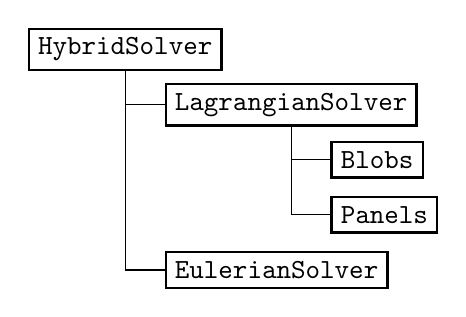
\begin{tikzpicture}[%
  grow via three points={one child at (0.5,-0.7) and
  two children at (0.5,-0.7) and (0.5,-1.4)},
  edge from parent path={(\tikzparentnode.south) |- (\tikzchildnode.west)}]
  \node {\texttt{HybridSolver}}
    child { node {\texttt{LagrangianSolver}}
    	child {node {\texttt{Blobs}}}
    	child {node {\texttt{Panels}}}  	
    }
    child [missing] {}				
    child [missing] {}				
    child { node {\texttt{EulerianSolver}}};
    %child { node [selected] {tex}
    %  child { node {generic}}
    %  child { node [optional] {latex}}
    %  child { node {plain}}
    %}
    %child [missing] {}
    %child { node {texdoc}};
\end{tikzpicture}
\end{figure}
%\end{abstract}
\newpage

\section*{\texttt{Blobs} Class}
The main structure of the \texttt{Blobs} class. This class contains all the function related to the calculation of the vortex blobs.
\begin{figure}[h]
\centering
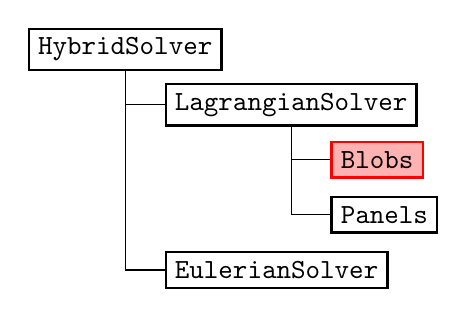
\begin{tikzpicture}[%
  grow via three points={one child at (0.5,-0.7) and
  two children at (0.5,-0.7) and (0.5,-1.4)},
  edge from parent path={(\tikzparentnode.south) |- (\tikzchildnode.west)}]
  \node {\texttt{HybridSolver}}
    child { node {\texttt{LagrangianSolver}}
    	child {node [selected] {\texttt{Blobs}}}
    	child {node {\texttt{Panels}}}  	
    }
    child [missing] {}				
    child [missing] {}				
    child { node {\texttt{EulerianSolver}}};
    %child { node [selected] {tex}
    %  child { node {generic}}
    %  child { node [optional] {latex}}
    %  child { node {plain}}
    %}
    %child [missing] {}
    %child { node {texdoc}};
\end{tikzpicture}
\end{figure}

\subsection*{Class structure:}
\begin{figure}[h]
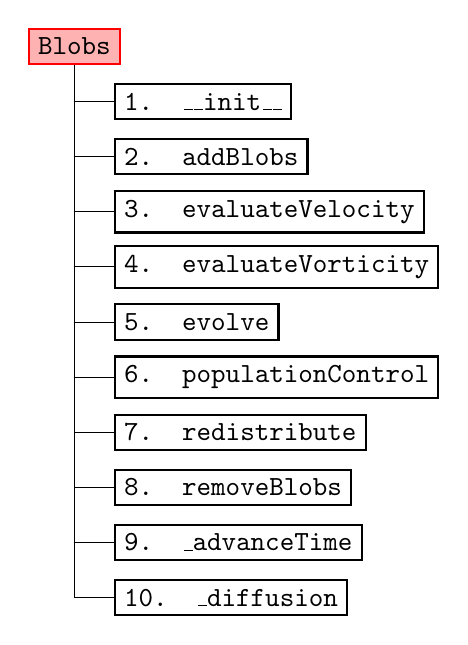
\begin{tikzpicture}[%
  grow via three points={one child at (0.5,-0.7) and
  two children at (0.5,-0.7) and (0.5,-1.4)},
  edge from parent path={(\tikzparentnode.south) |- (\tikzchildnode.west)}]
  \node [selected] {\texttt{Blobs}}
    child { node {\texttt{1. \_\_init\_\_}}}
    child { node {\texttt{2. addBlobs}}}
    child { node {\texttt{3. evaluateVelocity}}}                    
    child { node {\texttt{4. evaluateVorticity}}}   
    child { node {\texttt{5. evolve}}}    
    child { node {\texttt{6. populationControl}}}   
    child { node {\texttt{7. redistribute}}}    
	child { node {\texttt{8. removeBlobs}}}  
	child { node {\texttt{9. \_advanceTime}}}  	
	child { node {\texttt{10. \_diffusion}}};	
\end{tikzpicture}
\end{figure}

\subsection*{Attributes:}
\begingroup
\footnotesize
\begin{longtable}{|l|p{9cm}|}
	\hline
	\textbf{Attributes} & \textbf{Description}\\
	\toprule
    \texttt{blobControlParams} 		& The diffusion parameters. It is a dictionary containing all the parameters of the diffusion method used for the simulation. Contains: \texttt{stepRedistribution}, \texttt{stepPopulationControl}, \texttt{gThresholdLocal}, \texttt{gThresholdGlobal}.\\\hline
    \texttt{computationMethod} 		&\texttt{computationMethod} (tuple) with the type of Biot-Savart solver (\texttt{direct}, \texttt{fmm}) and the type of hardware to use (\texttt{cpu}, \texttt{gpu}).\\\hline
    \texttt{deltaTc} & The size of the convective time step $\Delta t_c$\\\hline
    \texttt{deltaTd} & The size of the convective time step $\Delta t_d$\\\hline
    \texttt{diffusionParams} & A dictionary containing all the parameters related to the computation of the diffusion step. Specifies the diffusion scheme and other specific parameters. Contains: \texttt{method}, \texttt{c2}.\\\hline
    \texttt{g} & The strength of the vortex blobs $\alpha$.\\          \hline
    \texttt{gThresholdGlobal} & Maximum value of variation of total vorticity due to the removal of blobs during population control.\\\hline
    \texttt{gThresholdLocal} & Minimum value of circulation to consider for each vortex blob when selecting blobs to remove during population control.\\    \hline      
    \texttt{h} & The size of the cell associated to the vortex blobs. Corresponds to the minimum spacing between the core of two neighboring cells. It is related to the core size of the blob, $\sigma$, and to the spacing $h$ by the expression $Ov = h/\sigma$.\\\hline          
    \texttt{integrationMethod} & \texttt{integrationMethod} (\texttt{fe}, \texttt{rk4}) the type of time integrator used: \texttt{fe} forward Euler, \texttt{rk4} Runge-Kutta $4^{th}$ order.\\ \hline
    \texttt{nu} & The fluid kinematic viscosity, used to calculate the diffusion coefficient: \texttt{c2} and diffusion time step \texttt{deltaTd}, $\Delta t_{d}$.\\          \hline
	\texttt{numBlobs} & The number of blobs.\\          \hline
	\texttt{overlap} & The overlap ratio between neighboring blobs.\\          \hline
	\texttt{plotVelocity} & A flag that defines if velocity is to be plotted or not.\\          \hline
	\texttt{sigma} & The core size of the vortex blobs.\\          \hline
	\texttt{stepDiffusion} & The frequency of diffusion steps.\\          \hline
	\texttt{stepPopulationControl} & The frequency of population control.\\          \hline
	\texttt{stepRedistribution} & The frequency of redistribution of blobs.\\          \hline
	\texttt{timeIntegrationParams} & A dictionary containing all time integration parameters of the simulation. Contains the definition of the time integration scheme possibly additional parameters specific to the scheme.\\ \hline
	\texttt{t} & The current time of the simulation.\\          \hline
	\texttt{tStep} & The current time step of the simulation.\\          \hline
	\texttt{velocityComputationParams} & A dictionary containing all the parameters related to the computation of induced velocities. Specifies computation scheme (direct or fmm) and hardware to use (cpu or gpu).\\          \hline
	\texttt{vInf} & The free stream velocity.\\          \hline
	\texttt{x} & The $x$ coordinates of the vortex blobs.\\          \hline
	\texttt{y} & The $y$ coordinates of the vortex blobs.\\          \hline	                                
    
                       
    \caption{Attributes of \texttt{Blobs} class and their description.}
    \label{tab:attributeBlobs}
\end{longtable}
\endgroup

\subsection*{\texttt{\_\_init\_\_}}
	\paragraph{Description:} Initialize the \texttt{Blobs} class with either the given input parameters or by a reading a \texttt{file} containing all the necessary parameters.\\
	
	\begin{tabular}{l|lp{7cm}}
		\multicolumn{2}{l}{\textbf{Input Parameters}} & \\ \hline
		\textit{File Name} & \multicolumn{2}{l}{Containing all the parameters to re-initalize the class.} \\ \cline{2-3}
		\multicolumn{3}{c}{--- or ---} \\ \cline{2-3}
		\multirow{4}{*}{\textit{Parameters}} & Vorticity Field &: \{\texttt{xBlob, yBlob, gBlob}\} or \{\texttt{wFunction, xBounds, yBounds}\}\\ \cline{2-3}
		& Blob parameters &: \texttt{overlap, h} \\ \cline{2-3}
		& Time Step parameters &: \texttt{deltaTc, nu, stepRedistribution, integrationMethod, computationMethod}\\ \cline{2-3}
		& Population control parameters &: \texttt{stepPopulationControl, gThreshold}\\ \cline{2-3}
	\end{tabular}\\
	
	\subsubsection*{Descriptions of the parameters:}
	\begin{tabular}{p{3.5cm}p{9cm}p{1cm}}
				\textit{Vorticity field} & & \textit{Default}\\ \hline
				\texttt{xBlob,yBlob} &:  the $x,y$ blob coordinates. & - \\
				\texttt{gBlob} &: the circulation $\Gamma_i$ associated to each of the vortex blobs. & - \\
				& & \\
				\multicolumn{2}{c}{\textit{--- or ---}} & \\
				& & \\
				\texttt{wExactFunction} &: the function that returns the exact value of vorticity $\omega$ at any given $x,y$ coordinates. &\\
				& 	\begin{tabular}{lp{10cm}}
						\textbf{Input parameters} &: \texttt{xEval,yEval}\\ 
						\textbf{Assigns} &: \texttt{-}\\ 			
						\textbf{Returns} &: \texttt{wEval}\\ 					
					\end{tabular} & - \\
				\texttt{xBounds, yBounds} &: the $x,y$ bounds of the domain where the particles was originally distributed. & - \\		 
	\end{tabular}\\
	\\ \\
	%	\begin{tabular}{lp{10cm}}
	%		\textbf{Input parameters} &: \texttt{xEval,yEval}\\ 
	%		\textbf{Assigns} &: \texttt{-}\\ 			
	%		\textbf{Returns} &: \texttt{vortEval}\\ 					
	%	\end{tabular}\\
	\begin{tabular}{p{3.5cm}p{9cm}p{1cm}}
				\multicolumn{2}{l}{\textit{Blob parameters}} & \textit{Default} \\ \hline				
				\texttt{overlap} &: the overlap ratio $h/\sigma$. & 1.0\\
				\texttt{h} &: the size of the cell $h$ associated to the blobs. \textit{Note:} Cells are square. & -\\
	\end{tabular}\\
	\\ \\
	\begin{tabular}{p{3.5cm}p{9cm}p{1cm}}
				\multicolumn{2}{l}{\textit{Time step parameters}} & \textit{Default}\\ \hline
				\texttt{deltaTc} &:  the size of the convective time step $\Delta t_c$. & - \\
				\texttt{nu} &: the fluid kinematic viscosity $\nu$, used to calculate the diffusion coefficient $c^2$ and diffusion time step size $\Delta T_d$.& - \\
				\texttt{stepRedistribution} &: the redistribution step frequency. & 1 \\
				\texttt{integrationMethod} &: the time integration method (\texttt{FE}: Forward euler , \texttt{RK4}: $4^{th}$ order Runge-Kutta). & RK4 \\
				\texttt{computationMethod} &: the calculation method to evolve the blobs, (\texttt{Direct}: Direct Method, \texttt{FMM}: Fast-Multipole Method) using (\texttt{CPU}, \texttt{GPU}). & \{FMM, GPU\}.\\
	\end{tabular}\\ 
    \\ \\ 
	\begin{tabular}{p{3.5cm}p{9cm}p{1cm}}
				\multicolumn{2}{l}{\textit{Population control parameters}} & \textit{Default} \\ \hline
				\texttt{stepPopulationControl} &: population control step frequency & 1.\\
				\texttt{gThreshold} &: the tuple with minimum \textbf{and} maximum value of the circulation $\Gamma_{min}$. & - \\
	\end{tabular}\\ 
    \\ \\  
	\begin{tabular}{p{3.5cm}p{9cm}p{1cm}}
				\multicolumn{2}{l}{\textit{Free stream velocity}} & \textit{Default}\\ \hline
				\texttt{vInf} &: The free-stream velocity function, returning the velocity action on the vortex blobs. & -\\		
				&		\begin{tabular}{lp{2cm}}
							\textbf{Input parameters} &: \texttt{t}\\ 
							\textbf{Assigns} &: \texttt{-}\\ 			
							\textbf{Returns} &: \texttt{vx,vy}\\ 					
						\end{tabular} & - \\
				
	\end{tabular}\\

\newpage
%%%%%%%%%%%%%%%%%%%%%%%%%%%%%%%%%%%%%%%%%%%%%%%%%%%%%%%%%%%%%%%%%%%%%%%%%%%%%%%%%%%%%%%%%%%%%%%%%%%%%%%%%%%%%%%%%%%%%%%%%%%%%%%%%%
%%%%%%%%%%%%%%%%%%%%%%%%%%%%%%%%%%%%%%%%%%%%%%%%%%%%%%%%%%%%%%%%%%%%%%%%%%%%%%%%%%%%%%%%%%%%%%%%%%%%%%%%%%%%%%%%%%%%%%%%%%%%%%%%%%

\section*{\texttt{Panels} class}
The main structure of the panel method class \texttt{Panels}. This class contains all the functions related to the calculation of panels.

\begin{figure}[h]
\centering
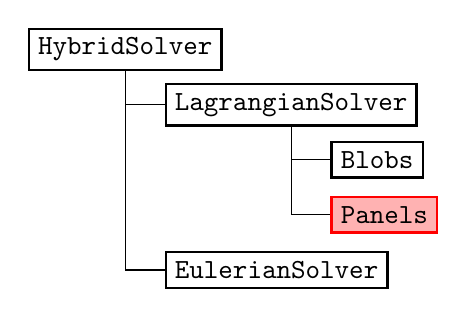
\begin{tikzpicture}[%
  grow via three points={one child at (0.5,-0.7) and
  two children at (0.5,-0.7) and (0.5,-1.4)},
  edge from parent path={(\tikzparentnode.south) |- (\tikzchildnode.west)}]
  \node {\texttt{HybridSolver}}
    child { node {\texttt{LagrangianSolver}}
    	child {node {\texttt{Blobs}}}
    	child {node [selected] {\texttt{Panels}}}  	
    }
    child [missing] {}				
    child [missing] {}				
    child { node {\texttt{EulerianSolver}}};
    %child { node [selected] {tex}
    %  child { node {generic}}
    %  child { node [optional] {latex}}
    %  child { node {plain}}
    %}
    %child [missing] {}
    %child { node {texdoc}};
\end{tikzpicture}
\end{figure}


\subsection*{Class structure:}
\begin{figure}[h]
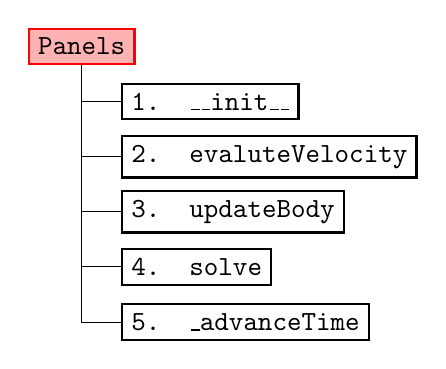
\begin{tikzpicture}[%
  grow via three points={one child at (0.5,-0.7) and
  two children at (0.5,-0.7) and (0.5,-1.4)},
  edge from parent path={(\tikzparentnode.south) |- (\tikzchildnode.west)}]
  \node [selected] {\texttt{Panels}}
    child { node {\texttt{1. \_\_init\_\_}}}
    child { node {\texttt{2. evaluteVelocity}}}                    
    child { node {\texttt{3. updateBody}}}                    
    child { node {\texttt{4. solve}}}                                        
    child { node {\texttt{5. \_advanceTime}}};
\end{tikzpicture}
\end{figure}


\subsection*{Attributes:}
\begingroup
\footnotesize
\begin{longtable}{|l|p{11cm}|}
	\hline
	\textbf{Attributes} & \textbf{Description}\\
	\toprule
    \texttt{A} 		& The inter-induction matrix $\mathbf{A}$, the LHS of the problem. \\ \hline
    \texttt{cmGlobal} & The global position vector for each of the $\mathbf{N}$
                       body, refining the position of the local panel $(0,0)$ in the
                       global coordinate system. \\\hline
    \texttt{deltaT} & The simulation time step size $\Delta T$\\ \hline
    \texttt{geometryKeys} & The dictionary containing all the parameters of the geometry. Contains: \texttt{xPanel} (the $x$ coordinate of the $\mathbf{M}$ panel corners.), \texttt{yPanel} (The $y$ coordinate of the $\mathbf{M}$ panel corners), \texttt{cmGlobal}, \texttt{thetaLocal}, \texttt{dPanel} (The off-set of the panel collocation point from the panel mid-point).  \\ \hline
    \texttt{nBodies} & The number of panel bodies.\\\hline
    \texttt{norm} & The $x$, $y$ normal vector of each panel.\\\hline
    \texttt{normCat} & The global concatenated $x$, $y$ component of the panel normal vector at each collocation points.\\          \hline
    \texttt{nPanels} & The number of panels in each body/geometry. \\ \hline
    \texttt{nPanelsTotal} & The total number of panels.\\    \hline      
    \texttt{panelKernel} & A string defining panel kernel type. \\\hline          
    \texttt{problemType} & A string defining the panel problem is of a \texttt{moving} type or of a \texttt{fixed} type.\\ \hline
    \texttt{solverCompParams} & The dictionary containing solver computation parameters.\\          \hline
	\texttt{sPanel} & The vortex sheet strengths $\gamma$ of $\mathbf{M}$ panels. \\          \hline
	\texttt{t} & The current time $t$ of the simulation.\\          \hline
	\texttt{tang} & The $x$, $y$ tangent vector of each panel.\\          \hline
	\texttt{tangCat} & The global concatenated $x$, $y$ component of the panel
	                  normal vector at each collocation points.\\          \hline
	\texttt{thetaLocal} & The local rotation angle $\theta$ w.r.t to the local
	                     coordinate system. The rotational will be performed around
	                     the local reference point $(0,0)$, i.e around the global center of rotation point \texttt{cmGlobal}.\\          \hline
	\texttt{tStep} & The current step of the simulation.\\          \hline
	\texttt{velCompParams} & A dictionary containing the velocity computation parameters, method and hardware.\\          \hline
	\texttt{xyCPGlobal} & The global $x$, $y$ coordinate of the panel collocation
	                     points.\\ \hline
	\texttt{xyCPGlobalCat} & The global concatenated $x$, $y$ coordinate of the
	                        panel collocation points.\\          \hline
	\texttt{xyPanelGlobal} & The global $x$, $y$ coordinate of the panel bodies.\\          \hline
	\texttt{xyPanelGlobalCat} & The global concatenated $x$, $y$ coordinate of the
	                           panel bodies.\\          \hline
	\texttt{xyPanelLocal} & The local $x$, $y$ coordinate of the panel bodies.\\          \hline
                       
    \caption{Attributes of \texttt{Panels} class and their description.}
    \label{tab:attributesPanels}
\end{longtable}
\endgroup


\subsection*{\texttt{\_\_init\_\_}}
	\begin{tabular}{l|lp{7cm}}
		\multicolumn{2}{l}{\textbf{Input Parameters}} & \\ \hline
		\textit{File Name} & \multicolumn{2}{l}{Containing all the parameters to re-initalize the class.} \\ \hline
		\multirow{2}{*}{\textit{Parameters}} & Panel coordinates &: \{\texttt{xCP, yCP, xPanel, yPanel, cmGlobal, thetaLocal}\}\\ \cline{2-3}
		& External velocity &: \texttt{externVel} \\ \cline{2-3}
	\end{tabular}
	\paragraph{Description:} Initialize the \texttt{panels} class with the given input parameters. In the case of a multibody problem, a list of panel coordinates can be given and internally it takes care of the inter-coupling.\\
	\\
	\begin{tabular}{lp{10cm}}
				\textit{Panel coordinates} & \\ \hline
				\texttt{xCP,yCP} &:  the local $x,y$-coordinates of the panel collocation points.\\ 
				\texttt{xPanel,yPanel} &: the local coordinate of the panel edges. \textit{Note}: Should have a closed loop (end with initial point coordinates).\\ 
				\texttt{cmGlobal} &:  the position of reference points of a given panel body.\\
				\texttt{thetaLocal} &:  the rotational angles of the panel body axes w.r.t to the global $x$-axis.\\
	\end{tabular}\\ 
    \\ \\
	\begin{tabular}{lp{10cm}}
				\textit{External velocity} & \\ \hline
				\texttt{externVel} &:  Reference to an external velocity \textbf{function} acting of the panels. For the panel case, the external velocity will the induced velocity of the blobs + freestream \texttt{vortexBlob.evaluateVelocity}.\\
	\end{tabular}\\
	
		\begin{tabular}{lp{10cm}}
			\textbf{Input parameters} &: \texttt{xCP,yCP}\\ 
			\textbf{Assigns} &: \texttt{-}\\ 			
			\textbf{Returns} &: \texttt{vxCP,vyCP}\\ 					
		\end{tabular}\\


\newpage
%%%%%%%%%%%%%%%%%%%%%%%%%%%%%%%%%%%%%%%%%%%%%%%%%%%%%%%%%%%%%%%%%%%%%%%%%%%%%%%%%%%%%%%%%%%%%%%%%%%%%%%%%%%%%%%%%%%%%%%%%%%%%%%%%%
%%%%%%%%%%%%%%%%%%%%%%%%%%%%%%%%%%%%%%%%%%%%%%%%%%%%%%%%%%%%%%%%%%%%%%%%%%%%%%%%%%%%%%%%%%%%%%%%%%%%%%%%%%%%%%%%%%%%%%%%%%%%%%%%%%

\section*{\texttt{LagrangianSolver} Class}
The main structure of the \texttt{Blobs} + \texttt{Panels} (LagrangianSolver) class. This class contains all the function related to the calculations of panel with vortex blobs.

\begin{figure}[h]
\centering
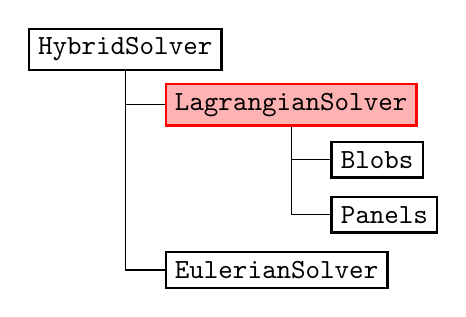
\begin{tikzpicture}[%
  grow via three points={one child at (0.5,-0.7) and
  two children at (0.5,-0.7) and (0.5,-1.4)},
  edge from parent path={(\tikzparentnode.south) |- (\tikzchildnode.west)}]
  \node {\texttt{HybridSolver}}
    child { node [selected] {\texttt{LagrangianSolver}}
    	child {node {\texttt{Blobs}}}
    	child {node {\texttt{Panels}}}  	
    }
    child [missing] {}				
    child [missing] {}				
    child { node {\texttt{EulerianSolver}}};
    %child { node [selected] {tex}
    %  child { node {generic}}
    %  child { node [optional] {latex}}
    %  child { node {plain}}
    %}
    %child [missing] {}
    %child { node {texdoc}};
\end{tikzpicture}
\end{figure}

\subsection*{Class structure:}
\begin{figure}[h]
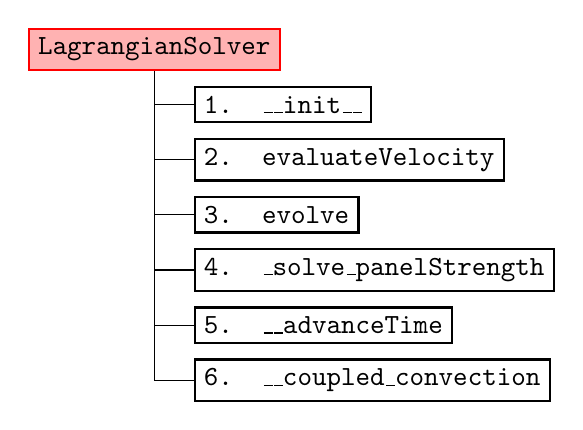
\begin{tikzpicture}[%
  grow via three points={one child at (0.5,-0.7) and
  two children at (0.5,-0.7) and (0.5,-1.4)},
  edge from parent path={(\tikzparentnode.south) |- (\tikzchildnode.west)}]
  \node [selected] {\texttt{LagrangianSolver}}
    child { node {\texttt{1. \_\_init\_\_}}}
    child { node {\texttt{2. evaluateVelocity}}}
    child { node {\texttt{3. evolve}}}
    child { node {\texttt{4. \_solve\_panelStrength}}}                        
    child { node {\texttt{5. \_\_advanceTime}}}                        
    child { node {\texttt{6. \_\_coupled\_convection}}};                       

\end{tikzpicture}
\end{figure}

\subsection*{Attributes:}
\begingroup
\footnotesize
\begin{longtable}{|l|p{12cm}|}
	\hline
	\textbf{Attributes} & \textbf{Description}\\
	\toprule
    \texttt{deltaT}     & The inter-induction matrix $\mathbf{A}$, the LHS of the problem. \\ \hline
    \texttt{gTotal}     & The total circulation of the Lagrangian domain. \\ \hline    
	\texttt{t} & The current time $t$ of the simulation.\\          \hline
	\texttt{tStep} & The current step of the simulation.\\          \hline
	\texttt{vInf} & The $x$, $y$ component of the free-stream velocity.\\          \hline	
	\texttt{Blobs} & The vortex blobs class \texttt{Blobs}.\\          \hline	
	\texttt{Panels} & The vortex panels class \texttt{Panels}.\\          \hline			
                      
    \caption{Attributes of \texttt{LagrangianSolver} class and their description.}
    \label{tab:attributesLagrangianSolver}
\end{longtable}
\endgroup


\subsection*{\texttt{\_\_init\_\_}}
	\begin{tabular}{l|lp{7cm}}
		\multicolumn{2}{l}{\textbf{Input Parameters}} & \\ \hline
		\textit{File Name} & \multicolumn{2}{l}{Containing all the parameters to re-initalize the class.} \\ \hline
		\multirow{2}{*}{\textit{Parameters}} & \texttt{vortexBlobs} &: \{\texttt{vortexBlobs}\} class. \\ \cline{2-3}
		& \texttt{panels} &: \texttt{panels} class. \\ \cline{2-3}
	\end{tabular}
	\paragraph{Description:} Initialize the \texttt{vortexMethod} class using \textbf{vortexBlob}+\textbf{panelMethod} \\ classes.
	\paragraph{Input parameters:}
	\begin{list}{\quad}{}
	\item \texttt{Blobs}: vortex particle class
	\item \texttt{Panels}: panel method class				
	\end{list}


\newpage
%%%%%%%%%%%%%%%%%%%%%%%%%%%%%%%%%%%%%%%%%%%%%%%%%%%%%%%%%%%%%%%%%%%%%%%%%%%%%%%%%%%%%%%%%%%%%%%%%%%%%%%%%%%%%%%%%%%%%%%%%%%%%%%%%%
%%%%%%%%%%%%%%%%%%%%%%%%%%%%%%%%%%%%%%%%%%%%%%%%%%%%%%%%%%%%%%%%%%%%%%%%%%%%%%%%%%%%%%%%%%%%%%%%%%%%%%%%%%%%%%%%%%%%%%%%%%%%%%%%%%

\section*{\texttt{EulerianSolver}}
The main structure for the Navier-stokes class \texttt{EulerianSolver}. This class contains all the functions related to computation of the Navier-stokes problem. Below is set of functions that acts as the interface to the class.

\begin{figure}[h]
\centering
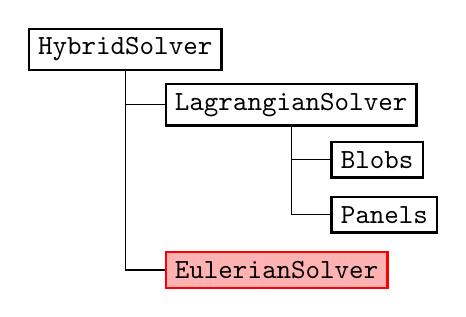
\begin{tikzpicture}[%
  grow via three points={one child at (0.5,-0.7) and
  two children at (0.5,-0.7) and (0.5,-1.4)},
  edge from parent path={(\tikzparentnode.south) |- (\tikzchildnode.west)}]
  \node {\texttt{HybridSolver}}
    child { node {\texttt{LagrangianSolver}}
    	child {node {\texttt{Blobs}}}
    	child {node {\texttt{Panels}}}  	
    }
    child [missing] {}				
    child [missing] {}				
    child { node [selected] {\texttt{EulerianSolver}}};
    %child { node [selected] {tex}
    %  child { node {generic}}
    %  child { node [optional] {latex}}
    %  child { node {plain}}
    %}
    %child [missing] {}
    %child { node {texdoc}};
\end{tikzpicture}
\end{figure}



\subsection*{Class structure:}
\begin{figure}[h]
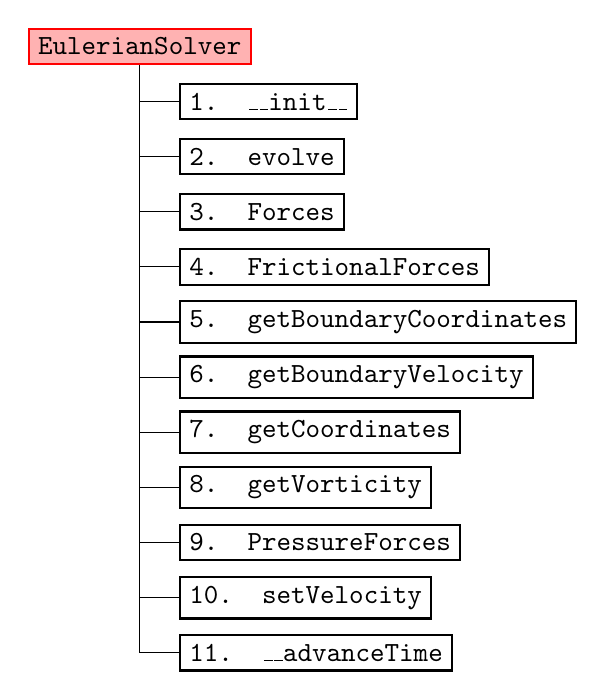
\begin{tikzpicture}[%
  grow via three points={one child at (0.5,-0.7) and
  two children at (0.5,-0.7) and (0.5,-1.4)},
  edge from parent path={(\tikzparentnode.south) |- (\tikzchildnode.west)}]
  \node [selected] {\texttt{EulerianSolver}}
    child { node {\texttt{1. \_\_init\_\_}}}
    child { node {\texttt{2. evolve}}}
    child { node {\texttt{3. Forces}}}
    child { node {\texttt{4. FrictionalForces}}}
    child { node {\texttt{5. getBoundaryCoordinates}}}                            
    child { node {\texttt{6. getBoundaryVelocity}}}                    
    child {node  {\texttt{7. getCoordinates}}}            
    child { node {\texttt{8. getVorticity}}}                                   
    child { node {\texttt{9. PressureForces}}}
    child { node {\texttt{10. setVelocity}}}
    child { node {\texttt{11. \_\_advanceTime}}};
\end{tikzpicture}
\end{figure}


\subsection*{Attributes:}
\begingroup
\footnotesize
\begin{longtable}{|l|p{11cm}|}
	\hline
	\textbf{Attributes} & \textbf{Description}\\
	\toprule
    \texttt{deltaT} 		& The time step size $\Delta t$. \\ \hline
    \texttt{deltaTMax} 		& The maximum allowable time step size $\max\{\Delta t\}$.\\ \hline
    \texttt{cfl} 			& The Courant–Friedrichs–Lewy condition stability number CFL. \\ \hline        
    \texttt{cmGlobal} 		& The $x$, $y$ position of the mesh local reference point $(0,0)$ in the global coordinates. \\ \hline        
    \texttt{hMin} 			& The minimum mesh cell size. \\ \hline        
    \texttt{nu} 			& The fluid kinematic viscosity $\nu$.  \\ \hline        
    \texttt{probeGridMesh} 	& The \textit{local} $x$, $y$ coordinates of the probe grid mesh. \\ \hline            
    \texttt{probeGridParams}& The dictionary containing all the parameters of the probe grid for extracting the vorticity data. \\ \hline            
    \texttt{solverParams} 	& The dictionary file containing all the solver parameters.  \\ \hline                
    \texttt{t} 				& The current time of the simulation. \\ \hline                    
    \texttt{thetaLocal} 	& The local rotational angle $\theta$ of the mesh domain. Therefore, the rotation will be done about local reference  point $(0,0)$, i.e \texttt{cmGlobal} in the global coordinate system.\\ \hline                            
    \texttt{tStep} 			& The current step of the simulation. \\ \hline                    
    \texttt{uMax} 			& The maximum fluid velocity $\max\{\mathbf{u}\}$. \\ \hline
    
    \caption{Attributes of \texttt{EulerianSolver} class and their description.}
    \label{tab:attributeEulerian}
\end{longtable}
\endgroup


\subsection*{\texttt{\_\_init\_\_}}
	\paragraph{Description:} Initialize the \texttt{navierStokes} class either using a \texttt{fileName} containing all the necessary parameter for initialization or by explicitly inputing the parameters.\\

	\begin{tabular}{l|lp{7cm}}
		\multicolumn{2}{l}{\textbf{Input Parameters}} & \\ \hline
		\textit{File Name} & \multicolumn{2}{l}{Containing all the parameters to re-initalize the class.} \\ \hline
		\multicolumn{3}{c}{-- or --} \\ \hline
		\multirow{5}{*}{\textit{Parameters}} & Mesh data &: \texttt{mesh, boundaryDomains}\\ \cline{2-3}
		& Geometry position &: \texttt{cmGlobal, thetaLocal} \\ \cline{2-3}
		& Fluid parameters &: \texttt{uMax, nu}\\ \cline{2-3}
		& Solver options &: \texttt{cfl}\\ \cline{2-3}
		& Probe grid parameters &: \texttt{x0, y0, Lx, Ly, hx, hy}\\ \cline{2-3}

	\end{tabular}\\
	\subsubsection*{Description of the parameters:}
	
	\begin{tabular}{lp{10cm}}
				\textit{Mesh data} & \\ \hline
				\texttt{mesh} &: the mesh data file.\\ 
				\texttt{boundaryDomains} &: the boundary mesh domain data file.\\ 			
	\end{tabular}\\ 
    \\ \\
	\begin{tabular}{lp{10cm}}
				\textit{Geometry position} & \\ \hline
				\texttt{cmGlobal} &: the $x,y$ position of the geometry in global coordinates.\\ 
				\texttt{thetaGlobal} &: the rotation angle (in $rad$) of the geometry in global coordinate system.\\ 			
	\end{tabular}\\
    \\ \\
	\begin{tabular}{lp{10cm}}
				\textit{Fluid parameters} & \\ \hline
				\texttt{uMax} &: the maximum fluid velocity $U_{max}$. Used to determine the maximum time step size $\Delta t_{max}$.\\ 
				\texttt{nu} &: the fluid kinematic viscosity $\nu$, for incompressible navier-stokes problem.\\ 			
	\end{tabular}\\	
    \\ \\
	\begin{tabular}{lp{10cm}}
				\textit{Solver options} & \\ \hline
				\texttt{cfl} &: the $CFL$ stability parameter. If explicit time marching scheme, $CFL<1$.\\ 		
	\end{tabular}\\	
    \\ \\
	\begin{tabular}{lp{10cm}}
				\textit{Probe grid parameters} & \\ \hline
				\texttt{x0,y0} &: the $x,y$ coordinate of the origin of the probe grid.\\ 
				\texttt{Lx,Ly} &: the $x,y$ size (width and height) of the probing grid.\\ 			
				\texttt{hx,hy} &: the $x,y$ spacing of the probe grid cell.\\ 							
	\end{tabular}\\	


\newpage
%%%%%%%%%%%%%%%%%%%%%%%%%%%%%%%%%%%%%%%%%%%%%%%%%%%%%%%%%%%%%%%%%%%%%%%%%%%%%%%%%%%%%%%%%%%%%%%%%%%%%%%%%%%%%%%%%%%%%%%%%%%%%%%%%%
%%%%%%%%%%%%%%%%%%%%%%%%%%%%%%%%%%%%%%%%%%%%%%%%%%%%%%%%%%%%%%%%%%%%%%%%%%%%%%%%%%%%%%%%%%%%%%%%%%%%%%%%%%%%%%%%%%%%%%%%%%%%%%%%%%


\section*{\texttt{HybridSolver} Class}
The main structure for the hybrid class \texttt{HybridSolver}. This class contains all the functions related to computation of the hybrid problem.

\begin{figure}[h]
\centering
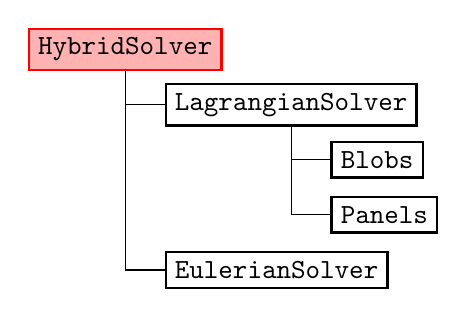
\begin{tikzpicture}[%
  grow via three points={one child at (0.5,-0.7) and
  two children at (0.5,-0.7) and (0.5,-1.4)},
  edge from parent path={(\tikzparentnode.south) |- (\tikzchildnode.west)}]
  \node [selected] {\texttt{HybridSolver}}
    child { node {\texttt{LagrangianSolver}}
    	child {node {\texttt{Blobs}}}
    	child {node {\texttt{Panels}}}  	
    }
    child [missing] {}				
    child [missing] {}				
    child { node {\texttt{EulerianSolver}}};
    %child { node [selected] {tex}
    %  child { node {generic}}
    %  child { node [optional] {latex}}
    %  child { node {plain}}
    %}
    %child [missing] {}
    %child { node {texdoc}};
\end{tikzpicture}
\end{figure}

\subsection*{Class structure:}
\begin{figure}[h]
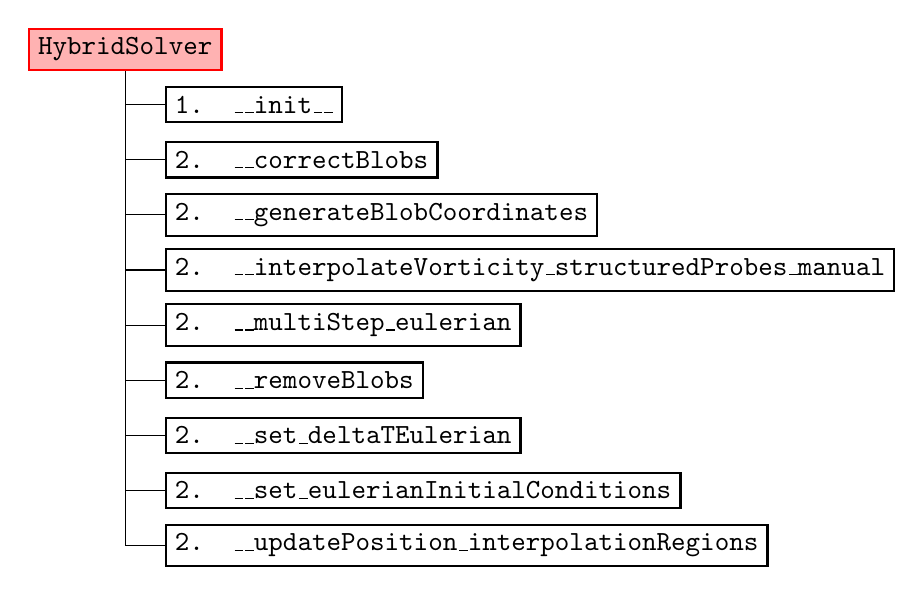
\begin{tikzpicture}[%
  grow via three points={one child at (0.5,-0.7) and
  two children at (0.5,-0.7) and (0.5,-1.4)},
  edge from parent path={(\tikzparentnode.south) |- (\tikzchildnode.west)}]
  \node [selected] {\texttt{HybridSolver}}
    child { node {\texttt{1. \_\_init\_\_}}}
    child { node {\texttt{2. \_\_correctBlobs}}}
    child { node {\texttt{2. \_\_generateBlobCoordinates}}}
    child { node {\texttt{2. \_\_interpolateVorticity\_structuredProbes\_manual}}}
    child { node {\texttt{2. \_\_multiStep\_eulerian}}}
    child { node {\texttt{2. \_\_removeBlobs}}}
    child { node {\texttt{2. \_\_set\_deltaTEulerian}}}    
    child { node {\texttt{2. \_\_set\_eulerianInitialConditions}}}        
    child { node {\texttt{2. \_\_updatePosition\_interpolationRegions}}};
\end{tikzpicture}
\end{figure}


\subsection*{Attributes:}
\begingroup
\footnotesize
\begin{longtable}{|l|p{10cm}|}
	\hline
	\textbf{Attributes} & \textbf{Description}\\
	\toprule
    \texttt{deltaTEulerian} 		& The time step size of the Eulerian sub-domain $\Delta t_E$. \\ \hline
    \texttt{deltaTLagrangian} 		& The time step size of the Lagrangian sub-domain $\Delta t_L$.\\ \hline
	\texttt{nu} 			& The fluid kinematic viscosity $\nu$.  \\ \hline        
    \texttt{t} 				& The current time $t$ of the simulation. \\ \hline                    
    \texttt{tStep} 			& The current step of the simulation. \\ \hline                    
    \texttt{vInf} 			& The $x$, $y$ component of the free-stream velocity. \\ \hline
    \texttt{interpolationRegion} & The dictionary containing the \texttt{surfacePolygon} and \texttt{boundaryPolygon} defining the boundaries of the interpolation region for each Eulerian sub-domains. The geometry is identified by the keys of the Eulerian sub-domain found in \texttt{multiEulerian}. The coordinates are defined in local coordinate system of the Eulerian grid and will be transformed (rotated + moved) during the evolution step. \\ \hline
    \texttt{lagrangian} 	& The Lagrangian solver class contains all the parameters related to simulation the flow in lagrangian sub-domain. \\ \hline
    \texttt{multiEulerian} 	& The \texttt{multiEulerian} is solver class containing all the Eulerian sub-domains of the hybrid problem. \\ \hline
    
    \caption{Attributes of \texttt{HybridSolver} class and their description.}
    \label{tab:attributeHybrid}
\end{longtable}
\endgroup


\subsection*{\texttt{\_\_init\_\_}}
	\begin{tabular}{l|lp{7cm}}
		\multicolumn{2}{l}{\textbf{Input Parameters}} & \\ \hline
		\textit{File Name} & \multicolumn{2}{l}{Containing all the parameters to re-initalize the class.} \\ \hline
		\multirow{4}{*}{\textit{Parameters}} & \texttt{vortexMethod} &: \{\texttt{vortexMethod}\} class.\\ \cline{2-3}
		& \texttt{navierStokes} &: \texttt{navierStokes} class. \\ \cline{2-3}
		& Interpolation region &: \texttt{xPolygon, yPolygon}\\ \cline{2-3}
		& Motion functions &: \texttt{T, cmGlobal, thetaGlobal, cmDotGlobal, thetaDotGlobal}\\ \cline{2-3}
	\end{tabular}\\
	
	\paragraph{Description:} Initialize the \texttt{hybrid} class using \texttt{LagrangianSolver} + \texttt{EulerianSolver} classes.
	\paragraph{Input parameters:}
	\begin{list}{\quad}{}
	\item \texttt{LagrangianSolver}: The vortex method containing \texttt{Blobs} and \textbf{Panels} classes which can already handle the multi-body problem.
	\item \texttt{EulerianSolver}: The Navier-Stokes grid solver class (if multiple: list of \\ \texttt{EulerianSolver} classes). The number of navier-stokes class has to be same as the number of vortex panels.
	\item \textbf{Interpolation Region}: the Navier-Stokes class (if multiple: list of \\ \texttt{EulerianSolver} classes). Should be equal to number of Navier-Stokes classes. The interpolation region should be defined as list of $x,y$ coordinates of the polygon of the interpolation region.
	\item \textbf{Motion function}: the function describing the motion of all the geometries in the hybrid class.
	\end{list}
	
	\begin{tabular}{lp{10cm}}
		\textit{Interpolation Regions} & \\ \hline
		\texttt{xPolygon,yPolygon}: & the new $x,y$ coordinate of the polygons description the interpolation region. The polygon should have a closed loop (end  with starting coordinates) before continuing to the next polygon. In the case of multiple polygons, a list of \texttt{xPolygon,yPolygon} should be given and should be as many as the number of navier-stokes domain.\\ 
	\end{tabular} \vspace{5 mm}

	\begin{tabular}{lp{10cm}}
		\textit{Motion function} & \\ \hline
		\texttt{T} &: the current time.\\ 
		\texttt{cmGlobal} &: a list of new positions of the geometries in the hybrid problem.\\ 
		\texttt{thetaGlobal} &: a list of new rotational angle of the geometries in the hybrid problem.\\ 		
		\texttt{cmDotGlobal} &: a list of current displacement velocity of the geometries in the hybrid problem.\\ 				
		\texttt{thetaDotGlobal} &: a list of current rotational velocity of the geometries in the hybrid problem.\\ 						
	\end{tabular} \vspace{5 mm}

	\begin{tabular}{lp{10cm}}
		\textbf{Input parameters} &: \texttt{T}\\ 
		\textbf{Assigns} &: \texttt{-}\\ 			
		\textbf{Returns} &: \texttt{cmGlobal,thetaGlobal,cmDotGlobal,thetaDotGlobal}\\ 					
	\end{tabular}



% Include all the documents
%\section{\texttt{vortexBlobs}}
The main structure of the \texttt{vortexBlobs} class. This class contains all the function related to the calculation of the vortex blobs.
\begin{figure}[h]
\centering
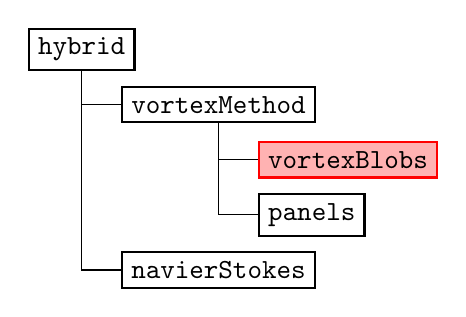
\begin{tikzpicture}[%
  grow via three points={one child at (0.5,-0.7) and
  two children at (0.5,-0.7) and (0.5,-1.4)},
  edge from parent path={(\tikzparentnode.south) |- (\tikzchildnode.west)}]
  \node {\texttt{hybrid}}
    child { node {\texttt{vortexMethod}}
    	child {node [selected] {\texttt{vortexBlobs}}}
    	child {node {\texttt{panels}}}  	
    }
    child [missing] {}				
    child [missing] {}				
    child { node {\texttt{navierStokes}}};
    %child { node [selected] {tex}
    %  child { node {generic}}
    %  child { node [optional] {latex}}
    %  child { node {plain}}
    %}
    %child [missing] {}
    %child { node {texdoc}};
\end{tikzpicture}
\end{figure}

\subsection*{Class structure:}
\begin{figure}[h]
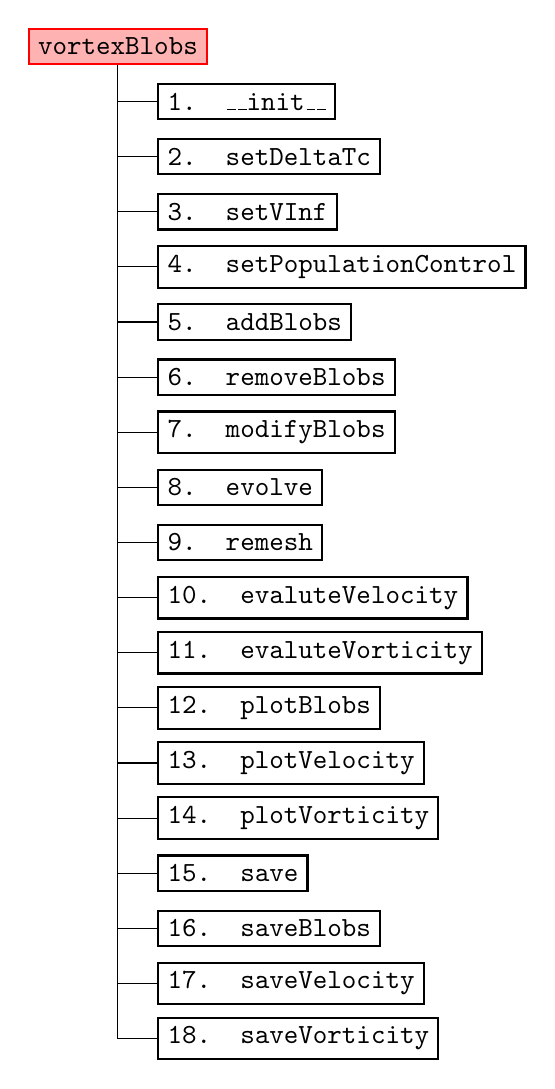
\begin{tikzpicture}[%
  grow via three points={one child at (0.5,-0.7) and
  two children at (0.5,-0.7) and (0.5,-1.4)},
  edge from parent path={(\tikzparentnode.south) |- (\tikzchildnode.west)}]
  \node [selected] {\texttt{vortexBlobs}}
    child { node {\texttt{1. \_\_init\_\_}}}
    child { node {\texttt{2. setDeltaTc}}}
    child { node {\texttt{3. setVInf}}}    
    child { node {\texttt{4. setPopulationControl}}}
    child { node {\texttt{5. addBlobs}}}
    child { node {\texttt{6. removeBlobs}}}    
    child { node {\texttt{7. modifyBlobs}}}    
    child { node {\texttt{8. evolve}}}    
    child { node {\texttt{9. remesh}}}    
    child { node {\texttt{10. evaluteVelocity}}}                    
    child { node {\texttt{11. evaluteVorticity}}}                        
    child { node {\texttt{12. plotBlobs}}}                        
    child { node {\texttt{13. plotVelocity}}}                        
    child { node {\texttt{14. plotVorticity}}}                            
    child { node {\texttt{15. save}}}                        
    child { node {\texttt{16. saveBlobs}}}                                        
    child { node {\texttt{17. saveVelocity}}}                                            
    child { node {\texttt{18. saveVorticity}}};
%    child { node [optional] {19. \texttt{\_generateBlobs}}}
%    child { node [optional] {20. \texttt{\_populationControl}}};        
        %child { node [selected] {tex}
    %  child { node {generic}}
    %  child { node [optional] {latex}}
    %  child { node {plain}}
    %}
    %child { node {texdoc}};
\end{tikzpicture}
\end{figure}

%\subsection*{Structure:}
%\begin{table}[h]
%\begin{tabular}{rl}
%	\texttt{vortexBlobs}: &  \\ \hline
%	-- & \texttt{\_\_init\_\_} \\
%	& \\
%	-- & \texttt{set\_deltaTc} \\ 
%	-- & \texttt{set\_popControlParameters} \\ 
%	-- & \texttt{addBlobs} \\ 
%	-- & \texttt{removeBlobs} \\ 
%	-- & \texttt{modifyBlobs} \\ 
%	-- & \texttt{evolve} \\ 
%	-- & \texttt{remesh} \\ 
%	-- & \texttt{evaluteVelocity} \\ 
%	-- & \texttt{evaluteVorticity} \\ 
%	-- & \texttt{plotBlobs} \\	
%	-- & \texttt{plotVelocity} \\
%	-- & \texttt{plotVorticity} \\
%	-- & \texttt{saveClass} \\ 
%	-- & \texttt{saveBlob} \\ 
%	-- & \texttt{saveVelocity} \\ 	
%	-- & \texttt{saveVorticity} \\ 
%	-- & \texttt{saveBlobPlot} \\ 
%	-- & \texttt{saveVelocityPlot} \\ 	
%	-- & \texttt{saveVorticityPlot} \\ 		
%	& \\
%	-- & \texttt{\_generateParticles} \\ 
%	-- & \texttt{\_popControl} \\
%\end{tabular}
%\end{table}

\newpage



\subsection{\texttt{\_\_init\_\_}}
	\paragraph{Description:} Initialize the \texttt{vortexBlobs} class with either the given input parameters or by a reading a \texttt{file} containing all the necessary parameters.\\
	
	\begin{tabular}{l|lp{7cm}}
		\multicolumn{2}{l}{\textbf{Input Parameters}} & \\ \hline
		\textit{File Name} & \multicolumn{2}{l}{Containing all the parameters to re-initalize the class.} \\ \cline{2-3}
		\multicolumn{3}{c}{--- or ---} \\ \cline{2-3}
		\multirow{4}{*}{\textit{Parameters}} & Vorticity Field &: \{\texttt{xBlob, yBlob, gBlob}\} or \{\texttt{wFunction, xBounds, yBounds}\}\\ \cline{2-3}
		& Blob parameters &: \texttt{overlap, h} \\ \cline{2-3}
		& Time Step parameters &: \texttt{deltaTc, nu, stepRedistribution, integrationMethod, computationMethod}\\ \cline{2-3}
		& Population control parameters &: \texttt{stepPopulationControl, gThreshold}\\ \cline{2-3}
	\end{tabular}\\
	
	\subsubsection*{Descriptions of the parameters:}
	\begin{tabular}{p{3.5cm}p{9cm}p{1cm}}
				\textit{Vorticity field} & & \textit{Default}\\ \hline
				\texttt{xBlob,yBlob} &:  the $x,y$ blob coordinates. & - \\
				\texttt{gBlob} &: the circulation $\Gamma_i$ associated to each of the vortex blobs. & - \\
				& & \\
				\multicolumn{2}{c}{\textit{--- or ---}} & \\
				& & \\
				\texttt{wExactFunction} &: the function that returns the exact value of vorticity $\omega$ at any given $x,y$ coordinates. &\\
				& 	\begin{tabular}{lp{10cm}}
						\textbf{Input parameters} &: \texttt{xEval,yEval}\\ 
						\textbf{Assigns} &: \texttt{-}\\ 			
						\textbf{Returns} &: \texttt{wEval}\\ 					
					\end{tabular} & - \\
				\texttt{xBounds, yBounds} &: the $x,y$ bounds of the domain where the particles was originally distributed. & - \\		 
	\end{tabular}\\
	\\ \\
	%	\begin{tabular}{lp{10cm}}
	%		\textbf{Input parameters} &: \texttt{xEval,yEval}\\ 
	%		\textbf{Assigns} &: \texttt{-}\\ 			
	%		\textbf{Returns} &: \texttt{vortEval}\\ 					
	%	\end{tabular}\\
	\begin{tabular}{p{3.5cm}p{9cm}p{1cm}}
				\multicolumn{2}{l}{\textit{Blob parameters}} & \textit{Default} \\ \hline				
				\texttt{overlap} &: the overlap ratio $h/\sigma$. & 1.0\\
				\texttt{h} &: the size of the cell $h$ associated to the blobs. \textit{Note:} Cells are square. & -\\
	\end{tabular}\\
	\\ \\
	\begin{tabular}{p{3.5cm}p{9cm}p{1cm}}
				\multicolumn{2}{l}{\textit{Time step parameters}} & \textit{Default}\\ \hline
				\texttt{deltaTc} &:  the size of the convective time step $\Delta t_c$. & - \\
				\texttt{nu} &: the fluid kinematic viscosity $\nu$, used to calculate the diffusion coefficient $c^2$ and diffusion time step size $\Delta T_d$.& - \\
				\texttt{stepRedistribution} &: the redistribution step frequency. & 1 \\
				\texttt{integrationMethod} &: the time integration method (\texttt{FE}: Forward euler , \texttt{RK4}: $4^{th}$ order Runge-Kutta). & RK4 \\
				\texttt{computationMethod} &: the calculation method to evolve the blobs, (\texttt{Direct}: Direct Method, \texttt{FMM}: Fast-Multipole Method) using (\texttt{CPU}, \texttt{GPU}). & \{FMM, GPU\}.\\
	\end{tabular}\\ 
    \\ \\ 
	\begin{tabular}{p{3.5cm}p{9cm}p{1cm}}
				\multicolumn{2}{l}{\textit{Population control parameters}} & \textit{Default} \\ \hline
				\texttt{stepPopulationControl} &: population control step frequency & 1.\\
				\texttt{gThreshold} &: the tuple with minimum \textbf{and} maximum value of the circulation $\Gamma_{min}$. & - \\
	\end{tabular}\\ 
    \\ \\  
	\begin{tabular}{p{3.5cm}p{9cm}p{1cm}}
				\multicolumn{2}{l}{\textit{Free stream velocity}} & \textit{Default}\\ \hline
				\texttt{vInf} &: The free-stream velocity function, returning the velocity action on the vortex blobs. & -\\		
				&		\begin{tabular}{lp{10cm}}
							\textbf{Input parameters} &: \texttt{t}\\ 
							\textbf{Assigns} &: \texttt{-}\\ 			
							\textbf{Returns} &: \texttt{vx,vy}\\ 					
						\end{tabular} & - \\
				
	\end{tabular}\\


\subsection{\texttt{setDeltaTc}}
	\paragraph{Description:} Function change the convective time step size $\Delta t_c$.\\
	
	 \begin{tabular}{p{3.5cm}p{10cm}p{1cm}}
				\multicolumn{2}{l}{\textit{Parameters}} & \textit{Default} \\ \hline
		   		\texttt{deltaTc} &: the new convection time step size $\Delta t_c$. & - \\
		\end{tabular} \vspace{5 mm}\\
	\\		
	\begin{tabular}{lp{10cm}}
		\textbf{Input parameters} &: \texttt{deltaTcNew}\\
		\textbf{Assigns} &:  \texttt{deltaTc}\\
		\textbf{Returns} &: \texttt{-}\\
	\end{tabular}

\subsection{\texttt{setPopulationControl}}
	\paragraph{Description:} function to modify the population control parameters.\\
	
	 \begin{tabular}{lp{10cm}}
				\textit{Parameters} & \\ \hline
		   		\texttt{gThresholdNew} &: the minimum and maximum circulation of the blobs, $\Gamma_{min}$\\
		   		\texttt{stepPopulationControlNew} &: the step number (frequency) of the population control.\\
		\end{tabular} \vspace{5 mm}\\
	\\		
	\begin{tabular}{lp{10cm}}
		\textbf{Input parameters} &: \texttt{gThresholdNew, stepPopulationControlNew}\\
		\textbf{Assigns} &:  \texttt{gThreshold, stepPopulationControl}\\
		\textbf{Returns} &: \texttt{-}\\
	\end{tabular}

		
\subsection{\texttt{addBlobs}}
	\paragraph{Description:} adds vortex particles by appending to the current set of particles.\\
	
	 \begin{tabular}{lp{10cm}}
				\textit{Parameters} & \\ \hline
		   		\texttt{xBlobNew,yBlobNew,gBlobNew} &: the coordinates and the strength of the new set of particles.\\
		\end{tabular} \vspace{5 mm}\\
	\\		
	\begin{tabular}{lp{10cm}}
		\textbf{Input parameters} &: \texttt{xBlobNew,yBlobNew,gBlobNew}\\
		\textbf{Assigns} &: \texttt{xBlob,yBlob,gBlob}\\
		\textbf{Returns} &: \texttt{-}\\
	\end{tabular}


\subsection{\texttt{removeBlobs}}
	\paragraph{Description:} removes vortex particles from the current set of particles. Using, the particle index, the associated $x,y$ and $\Gamma_i$ will be removed.\\
	
	 \begin{tabular}{lp{10cm}}
				\textit{Parameters} & \\ \hline
		   		\texttt{iBlob} &: the list of blob indices that is to be removed.\\
		\end{tabular} \vspace{5 mm}\\
	\\		
	\begin{tabular}{lp{10cm}}
		\textbf{Input parameters} &: \texttt{iBlob}\\
		\textbf{Assigns} &: \texttt{xBlob,yBlob,gBlob}\\
		\textbf{Returns} &: \texttt{-}\\
	\end{tabular}
	
	
\subsection{\texttt{modifyBlobs}}
	\paragraph{Description:} Replace the vortex particle strengths with the new strength.\\
	
	 \begin{tabular}{lp{10cm}}
				\textit{Parameters} & \\ \hline
		   		\texttt{iBlob} &: the list of blob indices that is to be modified.\\
		   		\texttt{gBlobNew} &: the new strength of the blobs.\\		   		
		\end{tabular} \vspace{5 mm}\\
	\\		
	\begin{tabular}{lp{10cm}}
		\textbf{Input parameters} &: \texttt{iBlob,gBlobNew}\\
		\textbf{Assigns} &: \texttt{gBlob}\\
		\textbf{Returns} &: \texttt{-}\\
	\end{tabular}	

\subsection{\texttt{evolve}}
	\paragraph{Description:} Evolves the vortex blobs according to the \texttt{\_\_init\_\_} definition. The \texttt{evolve} function, knows when (has a counter) to redistribute and perform population control. Depending on the diffusion time step $\Delta t_d$, the evolve function will also perform the diffusion process (modified interpolation).\\
	
	 \begin{tabular}{lp{10cm}}
				\textit{Parameters} & \\ \hline
		   		\texttt{xBlobNew,yBlobNew,gBlobNew} &: the new set of particle after the evolution process.\\
		\end{tabular} \vspace{5 mm}\\
	\\		
	\begin{tabular}{lp{10cm}}
		\textbf{Input parameters} &: \texttt{-}\\
		\textbf{Assigns} &: \texttt{xBlob,yBlob,gBlob}\\	
		\textbf{Returns} &: \texttt{-}\\
	\end{tabular}			


\subsection{\texttt{remesh}}
	\paragraph{Description:}  Function to remesh the particles on to the remeshing grid. When $c=0$, the remeshing will be done without diffusion. If $c>0$, the modified interpolation will perform the diffusion.
	\\
	\\		
	\begin{tabular}{lp{10cm}}
		\textbf{Input parameters} &: \texttt{c}\\ 
		\textbf{Assigns} &: \texttt{xBlob,yBlob,wBlob}\\ 			
		\textbf{Returns} &: \texttt{-}\\ 					
	\end{tabular}


\subsection{\texttt{evaluateVelocity}}
	\paragraph{Description:} Function to evaluate the total induced velocity due to the blobs, and the external velocity at a given target locations.\\
	
	    \begin{tabular}{lp{10cm}}
			\textit{Parameters} & \\ \hline
			 \texttt{xTarget,yTarget} &: the $x,y$ coordinate of the target location, where the total velocity is to be evaluated.\\
			\texttt{vxTarget,vyTarget} &: the $x,y$ induced velocity at the target points in global coordinate system.\\
		\end{tabular} \vspace{5 mm}
	\\		
	\begin{tabular}{lp{10cm}}
		\textbf{Input parameters} &: \texttt{xTarget,yTarget}\\ 
		\textbf{Assigns} &: \texttt{-}\\ 			
		\textbf{Returns} &: \texttt{vxTarget,vyTarget}\\ 					
	\end{tabular}	

\subsection{\texttt{evaluateVorticity}}
	\paragraph{Description:} Function to evaluate the total induced vorticity due to the blobs, and the external velocity at a given target coordinates.\\
	
	    \begin{tabular}{lp{10cm}}
			\textit{Parameters} & \\ \hline
			 \texttt{xTarget,yTarget} &: the $x,y$ coordinate of the target location, where the total velocity is to be evaluated.\\
			\texttt{wTarget} &: the $x,y$ induced vorticity at the target points in global coordinate system.\\
		\end{tabular} \vspace{5 mm}
	\\		
	\begin{tabular}{lp{10cm}}
		\textbf{Input parameters} &: \texttt{xTarget,yTarget}\\ 
		\textbf{Assigns} &: \texttt{-}\\ 			
		\textbf{Returns} &: \texttt{wTarget}\\ 					
	\end{tabular}


		
\subsection{plots \ldots}
	\paragraph{Description:} functions to plot and/or save all the results in a given region. The data should be store for scientific visualization (paraview format)\\
	
		\begin{tabular}{lp{10cm}}
			\textit{Plot variables:} & \\ \hline
			\texttt{plotBlob} &: plot the coordinates and the circulation of the blobs.\\
			\texttt{plotVelocity} &: plot the velocity field.\\ 
			\texttt{plotVorticity} &: plot the vorticity field.\\ 
		\end{tabular} \vspace{5 mm}
		
		\begin{tabular}{lp{10cm}}
			\textit{Parameters:} & \\ \hline
			\texttt{xBounds,yBounds} &: $x,y$ bounds of the grid, where the data is to be evaluated.\\ 
			\texttt{nGrid} &: $x,y$ number of grid points.\\
		\end{tabular} \vspace{5 mm}\\
	\\
	\begin{tabular}{lp{10cm}}
		\textbf{Input parameters} &: \texttt{xBounds,yBounds,nGrid}\\
		\textbf{Assigns} &: \texttt{-}\\ 			
		\textbf{Returns} &: \texttt{figureHandle} or \texttt{.pvd}\\ 					
	\end{tabular}	

\subsection{save data \ldots}
	\paragraph{Description:} functions to save the data. The data file will be in compressed, binary format to store efficiently.\\

		\begin{tabular}{lp{10cm}}
			\textit{Save variables:} & \\ \hline
			\texttt{save} &: all the data of the \texttt{vortexBlob} class is saved. This can be used later to restart the problem, i.e the parameter to init the problem.\\
			\texttt{saveBlobs} &: the function to save the blob data at the current time instant. List of numpy array.\\ 			
			\texttt{saveVelocity} &: save the velocity field of a given region or a given set of points.\\ 
			\texttt{saveVorticity} &: save the vorticity field of the given region or the given set of points.\\ 
		\end{tabular} \vspace{5 mm}
	
		\begin{tabular}{lp{10cm}}
			\textit{Parameters:} & \\ \hline
			\texttt{xBounds,yBounds} &: $x,y$ bounds of the grid, where the data is to be evaluated and saved.\\ 
			\texttt{nGrid} &: $x,y$ number of grid points.\\
			\texttt{xEval,yEval} &: $x,y$ coordinates of the location where the data is to be evaluated and saved.\\ 
		\end{tabular} \vspace{5 mm}\\
	\\
	\begin{tabular}{lp{10cm}}
		\textbf{Input parameters} &: \texttt{xBounds,yBounds,hGrid} or \texttt{xEval,yEval}\\ 
		\textbf{Assigns} &: \texttt{-}\\ 			
		\textbf{Returns} &: \texttt{.npz, .bin or similar}\\ 					
	\end{tabular}



%\subsection{save plots \ldots}
%	\paragraph{Description:} Function to save the plots as scientific visualization format \texttt{.pvd}.\\
%	
%		\begin{tabular}{lp{10cm}}
%			\textit{Save variables:} & \\ \hline
%			\texttt{saveBlobPlot} &: save the particle position and strengths as glyphs.\\
%			\texttt{saveVelocityPlot} &: save the velocity plot of a given region.\\ 
%			\texttt{saveVorticityPlot} &: save the vorticity of a given region.\\ 
%		\end{tabular} \vspace{5 mm}
%		
%		\begin{tabular}{lp{10cm}}
%			\textit{Parameters:} & \\ \hline
%			\texttt{xBounds,yBounds} &: $x,y$ bounds of the grid, where the data is to be evaluated and saved.\\ 
%			\texttt{hGrid} &: $x,y$ spacing of the evaluation grid.\\
%		\end{tabular} \vspace{5 mm}\\
%	\\
%	\begin{tabular}{lp{10cm}}
%		\textbf{Input parameters} &: \texttt{xBounds,yBounds,hGrid}\\
%		\textbf{Assigns} &: \texttt{-}\\ 			
%		\textbf{Returns} &: \texttt{.pvd}\\ 					
%	\end{tabular}
	


%\subsection{\texttt{\_generateParticles}}
%	\paragraph{Description:} \textit{Internal} function to generate/initialize the particles.\\
%	\\
%	\\
%		\begin{tabular}{lp{10cm}}
%			\textbf{Input parameters} &: \texttt{wExactFunction, xBounds, yBounds}\\ 
%			\textbf{Assigns} &: \texttt{xBlob,yBlob,wBlob}\\ 			
%			\textbf{Returns} &: \texttt{-}\\ 					
%		\end{tabular}	
%
%
%\subsection{\texttt{\_popControl}}
%	\paragraph{Description:} \textit{Internal} function to perform population control on the current set of particles.\\
%	\\
%	\\	
%		\begin{tabular}{lp{10cm}}
%			\textbf{Input parameters} &: \texttt{-}\\ 
%			\textbf{Assigns} &: \texttt{xBlob,yBlob,wBlob}\\ 			
%			\textbf{Returns} &: \texttt{-}\\ 					
%		\end{tabular}	
%\section{\texttt{vortexBlobs}}
The main structure of the \texttt{vortexBlobs} class. This class contains all the function related to the calculation of the vortex blobs.
\begin{figure}[h]
\centering
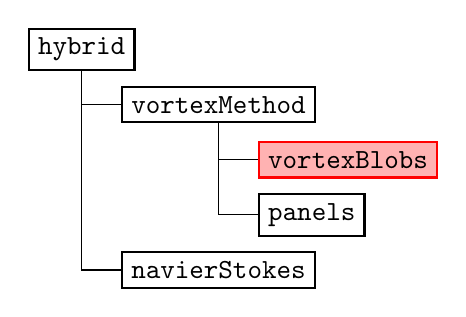
\begin{tikzpicture}[%
  grow via three points={one child at (0.5,-0.7) and
  two children at (0.5,-0.7) and (0.5,-1.4)},
  edge from parent path={(\tikzparentnode.south) |- (\tikzchildnode.west)}]
  \node {\texttt{hybrid}}
    child { node {\texttt{vortexMethod}}
    	child {node [selected] {\texttt{vortexBlobs}}}
    	child {node {\texttt{panels}}}  	
    }
    child [missing] {}				
    child [missing] {}				
    child { node {\texttt{navierStokes}}};
    %child { node [selected] {tex}
    %  child { node {generic}}
    %  child { node [optional] {latex}}
    %  child { node {plain}}
    %}
    %child [missing] {}
    %child { node {texdoc}};
\end{tikzpicture}
\end{figure}

\subsection*{Class structure:}
\begin{figure}[h]
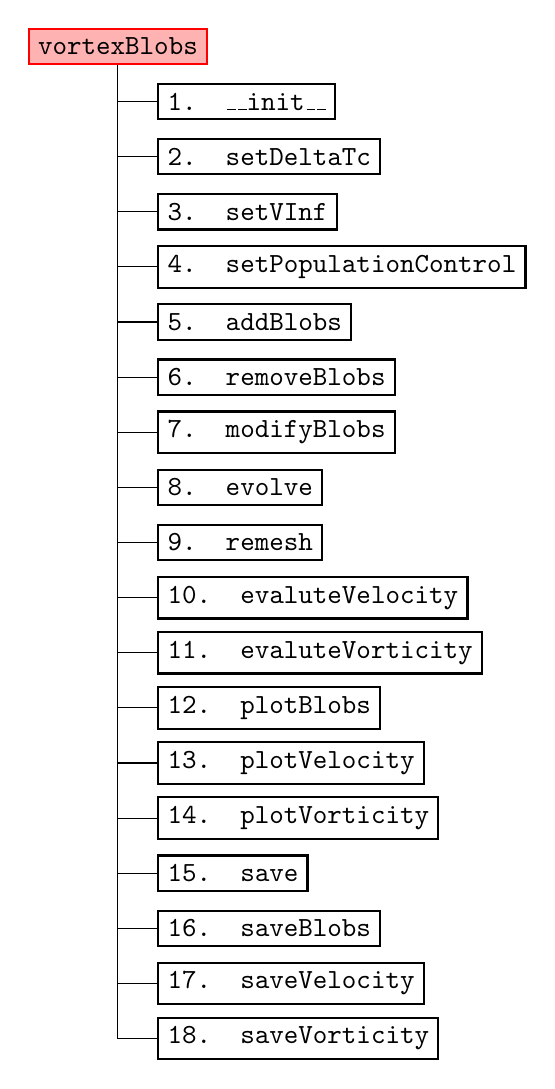
\begin{tikzpicture}[%
  grow via three points={one child at (0.5,-0.7) and
  two children at (0.5,-0.7) and (0.5,-1.4)},
  edge from parent path={(\tikzparentnode.south) |- (\tikzchildnode.west)}]
  \node [selected] {\texttt{vortexBlobs}}
    child { node {\texttt{1. \_\_init\_\_}}}
    child { node {\texttt{2. setDeltaTc}}}
    child { node {\texttt{3. setVInf}}}    
    child { node {\texttt{4. setPopulationControl}}}
    child { node {\texttt{5. addBlobs}}}
    child { node {\texttt{6. removeBlobs}}}    
    child { node {\texttt{7. modifyBlobs}}}    
    child { node {\texttt{8. evolve}}}    
    child { node {\texttt{9. remesh}}}    
    child { node {\texttt{10. evaluteVelocity}}}                    
    child { node {\texttt{11. evaluteVorticity}}}                        
    child { node {\texttt{12. plotBlobs}}}                        
    child { node {\texttt{13. plotVelocity}}}                        
    child { node {\texttt{14. plotVorticity}}}                            
    child { node {\texttt{15. save}}}                        
    child { node {\texttt{16. saveBlobs}}}                                        
    child { node {\texttt{17. saveVelocity}}}                                            
    child { node {\texttt{18. saveVorticity}}};
%    child { node [optional] {19. \texttt{\_generateBlobs}}}
%    child { node [optional] {20. \texttt{\_populationControl}}};        
        %child { node [selected] {tex}
    %  child { node {generic}}
    %  child { node [optional] {latex}}
    %  child { node {plain}}
    %}
    %child { node {texdoc}};
\end{tikzpicture}
\end{figure}

%\subsection*{Structure:}
%\begin{table}[h]
%\begin{tabular}{rl}
%	\texttt{vortexBlobs}: &  \\ \hline
%	-- & \texttt{\_\_init\_\_} \\
%	& \\
%	-- & \texttt{set\_deltaTc} \\ 
%	-- & \texttt{set\_popControlParameters} \\ 
%	-- & \texttt{addBlobs} \\ 
%	-- & \texttt{removeBlobs} \\ 
%	-- & \texttt{modifyBlobs} \\ 
%	-- & \texttt{evolve} \\ 
%	-- & \texttt{remesh} \\ 
%	-- & \texttt{evaluteVelocity} \\ 
%	-- & \texttt{evaluteVorticity} \\ 
%	-- & \texttt{plotBlobs} \\	
%	-- & \texttt{plotVelocity} \\
%	-- & \texttt{plotVorticity} \\
%	-- & \texttt{saveClass} \\ 
%	-- & \texttt{saveBlob} \\ 
%	-- & \texttt{saveVelocity} \\ 	
%	-- & \texttt{saveVorticity} \\ 
%	-- & \texttt{saveBlobPlot} \\ 
%	-- & \texttt{saveVelocityPlot} \\ 	
%	-- & \texttt{saveVorticityPlot} \\ 		
%	& \\
%	-- & \texttt{\_generateParticles} \\ 
%	-- & \texttt{\_popControl} \\
%\end{tabular}
%\end{table}

\newpage



\subsection{\texttt{\_\_init\_\_}}
	\paragraph{Description:} Initialize the \texttt{vortexBlobs} class with either the given input parameters or by a reading a \texttt{file} containing all the necessary parameters.\\
	
	\begin{tabular}{l|lp{7cm}}
		\multicolumn{2}{l}{\textbf{Input Parameters}} & \\ \hline
		\textit{File Name} & \multicolumn{2}{l}{Containing all the parameters to re-initalize the class.} \\ \cline{2-3}
		\multicolumn{3}{c}{--- or ---} \\ \cline{2-3}
		\multirow{4}{*}{\textit{Parameters}} & Vorticity Field &: \{\texttt{xBlob, yBlob, gBlob}\} or \{\texttt{wFunction, xBounds, yBounds}\}\\ \cline{2-3}
		& Blob parameters &: \texttt{overlap, h} \\ \cline{2-3}
		& Time Step parameters &: \texttt{deltaTc, nu, stepRedistribution, integrationMethod, computationMethod}\\ \cline{2-3}
		& Population control parameters &: \texttt{stepPopulationControl, gThreshold}\\ \cline{2-3}
	\end{tabular}\\
	
	\subsubsection*{Descriptions of the parameters:}
	\begin{tabular}{p{3.5cm}p{9cm}p{1cm}}
				\textit{Vorticity field} & & \textit{Default}\\ \hline
				\texttt{xBlob,yBlob} &:  the $x,y$ blob coordinates. & - \\
				\texttt{gBlob} &: the circulation $\Gamma_i$ associated to each of the vortex blobs. & - \\
				& & \\
				\multicolumn{2}{c}{\textit{--- or ---}} & \\
				& & \\
				\texttt{wExactFunction} &: the function that returns the exact value of vorticity $\omega$ at any given $x,y$ coordinates. &\\
				& 	\begin{tabular}{lp{10cm}}
						\textbf{Input parameters} &: \texttt{xEval,yEval}\\ 
						\textbf{Assigns} &: \texttt{-}\\ 			
						\textbf{Returns} &: \texttt{wEval}\\ 					
					\end{tabular} & - \\
				\texttt{xBounds, yBounds} &: the $x,y$ bounds of the domain where the particles was originally distributed. & - \\		 
	\end{tabular}\\
	\\ \\
	%	\begin{tabular}{lp{10cm}}
	%		\textbf{Input parameters} &: \texttt{xEval,yEval}\\ 
	%		\textbf{Assigns} &: \texttt{-}\\ 			
	%		\textbf{Returns} &: \texttt{vortEval}\\ 					
	%	\end{tabular}\\
	\begin{tabular}{p{3.5cm}p{9cm}p{1cm}}
				\multicolumn{2}{l}{\textit{Blob parameters}} & \textit{Default} \\ \hline				
				\texttt{overlap} &: the overlap ratio $h/\sigma$. & 1.0\\
				\texttt{h} &: the size of the cell $h$ associated to the blobs. \textit{Note:} Cells are square. & -\\
	\end{tabular}\\
	\\ \\
	\begin{tabular}{p{3.5cm}p{9cm}p{1cm}}
				\multicolumn{2}{l}{\textit{Time step parameters}} & \textit{Default}\\ \hline
				\texttt{deltaTc} &:  the size of the convective time step $\Delta t_c$. & - \\
				\texttt{nu} &: the fluid kinematic viscosity $\nu$, used to calculate the diffusion coefficient $c^2$ and diffusion time step size $\Delta T_d$.& - \\
				\texttt{stepRedistribution} &: the redistribution step frequency. & 1 \\
				\texttt{integrationMethod} &: the time integration method (\texttt{FE}: Forward euler , \texttt{RK4}: $4^{th}$ order Runge-Kutta). & RK4 \\
				\texttt{computationMethod} &: the calculation method to evolve the blobs, (\texttt{Direct}: Direct Method, \texttt{FMM}: Fast-Multipole Method) using (\texttt{CPU}, \texttt{GPU}). & \{FMM, GPU\}.\\
	\end{tabular}\\ 
    \\ \\ 
	\begin{tabular}{p{3.5cm}p{9cm}p{1cm}}
				\multicolumn{2}{l}{\textit{Population control parameters}} & \textit{Default} \\ \hline
				\texttt{stepPopulationControl} &: population control step frequency & 1.\\
				\texttt{gThreshold} &: the tuple with minimum \textbf{and} maximum value of the circulation $\Gamma_{min}$. & - \\
	\end{tabular}\\ 
    \\ \\  
	\begin{tabular}{p{3.5cm}p{9cm}p{1cm}}
				\multicolumn{2}{l}{\textit{Free stream velocity}} & \textit{Default}\\ \hline
				\texttt{vInf} &: The free-stream velocity function, returning the velocity action on the vortex blobs. & -\\		
				&		\begin{tabular}{lp{10cm}}
							\textbf{Input parameters} &: \texttt{t}\\ 
							\textbf{Assigns} &: \texttt{-}\\ 			
							\textbf{Returns} &: \texttt{vx,vy}\\ 					
						\end{tabular} & - \\
				
	\end{tabular}\\


\subsection{\texttt{setDeltaTc}}
	\paragraph{Description:} Function change the convective time step size $\Delta t_c$.\\
	
	 \begin{tabular}{p{3.5cm}p{10cm}p{1cm}}
				\multicolumn{2}{l}{\textit{Parameters}} & \textit{Default} \\ \hline
		   		\texttt{deltaTc} &: the new convection time step size $\Delta t_c$. & - \\
		\end{tabular} \vspace{5 mm}\\
	\\		
	\begin{tabular}{lp{10cm}}
		\textbf{Input parameters} &: \texttt{deltaTcNew}\\
		\textbf{Assigns} &:  \texttt{deltaTc}\\
		\textbf{Returns} &: \texttt{-}\\
	\end{tabular}

\subsection{\texttt{setPopulationControl}}
	\paragraph{Description:} function to modify the population control parameters.\\
	
	 \begin{tabular}{lp{10cm}}
				\textit{Parameters} & \\ \hline
		   		\texttt{gThresholdNew} &: the minimum and maximum circulation of the blobs, $\Gamma_{min}$\\
		   		\texttt{stepPopulationControlNew} &: the step number (frequency) of the population control.\\
		\end{tabular} \vspace{5 mm}\\
	\\		
	\begin{tabular}{lp{10cm}}
		\textbf{Input parameters} &: \texttt{gThresholdNew, stepPopulationControlNew}\\
		\textbf{Assigns} &:  \texttt{gThreshold, stepPopulationControl}\\
		\textbf{Returns} &: \texttt{-}\\
	\end{tabular}

		
\subsection{\texttt{addBlobs}}
	\paragraph{Description:} adds vortex particles by appending to the current set of particles.\\
	
	 \begin{tabular}{lp{10cm}}
				\textit{Parameters} & \\ \hline
		   		\texttt{xBlobNew,yBlobNew,gBlobNew} &: the coordinates and the strength of the new set of particles.\\
		\end{tabular} \vspace{5 mm}\\
	\\		
	\begin{tabular}{lp{10cm}}
		\textbf{Input parameters} &: \texttt{xBlobNew,yBlobNew,gBlobNew}\\
		\textbf{Assigns} &: \texttt{xBlob,yBlob,gBlob}\\
		\textbf{Returns} &: \texttt{-}\\
	\end{tabular}


\subsection{\texttt{removeBlobs}}
	\paragraph{Description:} removes vortex particles from the current set of particles. Using, the particle index, the associated $x,y$ and $\Gamma_i$ will be removed.\\
	
	 \begin{tabular}{lp{10cm}}
				\textit{Parameters} & \\ \hline
		   		\texttt{iBlob} &: the list of blob indices that is to be removed.\\
		\end{tabular} \vspace{5 mm}\\
	\\		
	\begin{tabular}{lp{10cm}}
		\textbf{Input parameters} &: \texttt{iBlob}\\
		\textbf{Assigns} &: \texttt{xBlob,yBlob,gBlob}\\
		\textbf{Returns} &: \texttt{-}\\
	\end{tabular}
	
	
\subsection{\texttt{modifyBlobs}}
	\paragraph{Description:} Replace the vortex particle strengths with the new strength.\\
	
	 \begin{tabular}{lp{10cm}}
				\textit{Parameters} & \\ \hline
		   		\texttt{iBlob} &: the list of blob indices that is to be modified.\\
		   		\texttt{gBlobNew} &: the new strength of the blobs.\\		   		
		\end{tabular} \vspace{5 mm}\\
	\\		
	\begin{tabular}{lp{10cm}}
		\textbf{Input parameters} &: \texttt{iBlob,gBlobNew}\\
		\textbf{Assigns} &: \texttt{gBlob}\\
		\textbf{Returns} &: \texttt{-}\\
	\end{tabular}	

\subsection{\texttt{evolve}}
	\paragraph{Description:} Evolves the vortex blobs according to the \texttt{\_\_init\_\_} definition. The \texttt{evolve} function, knows when (has a counter) to redistribute and perform population control. Depending on the diffusion time step $\Delta t_d$, the evolve function will also perform the diffusion process (modified interpolation).\\
	
	 \begin{tabular}{lp{10cm}}
				\textit{Parameters} & \\ \hline
		   		\texttt{xBlobNew,yBlobNew,gBlobNew} &: the new set of particle after the evolution process.\\
		\end{tabular} \vspace{5 mm}\\
	\\		
	\begin{tabular}{lp{10cm}}
		\textbf{Input parameters} &: \texttt{-}\\
		\textbf{Assigns} &: \texttt{xBlob,yBlob,gBlob}\\	
		\textbf{Returns} &: \texttt{-}\\
	\end{tabular}			


\subsection{\texttt{remesh}}
	\paragraph{Description:}  Function to remesh the particles on to the remeshing grid. When $c=0$, the remeshing will be done without diffusion. If $c>0$, the modified interpolation will perform the diffusion.
	\\
	\\		
	\begin{tabular}{lp{10cm}}
		\textbf{Input parameters} &: \texttt{c}\\ 
		\textbf{Assigns} &: \texttt{xBlob,yBlob,wBlob}\\ 			
		\textbf{Returns} &: \texttt{-}\\ 					
	\end{tabular}


\subsection{\texttt{evaluateVelocity}}
	\paragraph{Description:} Function to evaluate the total induced velocity due to the blobs, and the external velocity at a given target locations.\\
	
	    \begin{tabular}{lp{10cm}}
			\textit{Parameters} & \\ \hline
			 \texttt{xTarget,yTarget} &: the $x,y$ coordinate of the target location, where the total velocity is to be evaluated.\\
			\texttt{vxTarget,vyTarget} &: the $x,y$ induced velocity at the target points in global coordinate system.\\
		\end{tabular} \vspace{5 mm}
	\\		
	\begin{tabular}{lp{10cm}}
		\textbf{Input parameters} &: \texttt{xTarget,yTarget}\\ 
		\textbf{Assigns} &: \texttt{-}\\ 			
		\textbf{Returns} &: \texttt{vxTarget,vyTarget}\\ 					
	\end{tabular}	

\subsection{\texttt{evaluateVorticity}}
	\paragraph{Description:} Function to evaluate the total induced vorticity due to the blobs, and the external velocity at a given target coordinates.\\
	
	    \begin{tabular}{lp{10cm}}
			\textit{Parameters} & \\ \hline
			 \texttt{xTarget,yTarget} &: the $x,y$ coordinate of the target location, where the total velocity is to be evaluated.\\
			\texttt{wTarget} &: the $x,y$ induced vorticity at the target points in global coordinate system.\\
		\end{tabular} \vspace{5 mm}
	\\		
	\begin{tabular}{lp{10cm}}
		\textbf{Input parameters} &: \texttt{xTarget,yTarget}\\ 
		\textbf{Assigns} &: \texttt{-}\\ 			
		\textbf{Returns} &: \texttt{wTarget}\\ 					
	\end{tabular}


		
\subsection{plots \ldots}
	\paragraph{Description:} functions to plot and/or save all the results in a given region. The data should be store for scientific visualization (paraview format)\\
	
		\begin{tabular}{lp{10cm}}
			\textit{Plot variables:} & \\ \hline
			\texttt{plotBlob} &: plot the coordinates and the circulation of the blobs.\\
			\texttt{plotVelocity} &: plot the velocity field.\\ 
			\texttt{plotVorticity} &: plot the vorticity field.\\ 
		\end{tabular} \vspace{5 mm}
		
		\begin{tabular}{lp{10cm}}
			\textit{Parameters:} & \\ \hline
			\texttt{xBounds,yBounds} &: $x,y$ bounds of the grid, where the data is to be evaluated.\\ 
			\texttt{nGrid} &: $x,y$ number of grid points.\\
		\end{tabular} \vspace{5 mm}\\
	\\
	\begin{tabular}{lp{10cm}}
		\textbf{Input parameters} &: \texttt{xBounds,yBounds,nGrid}\\
		\textbf{Assigns} &: \texttt{-}\\ 			
		\textbf{Returns} &: \texttt{figureHandle} or \texttt{.pvd}\\ 					
	\end{tabular}	

\subsection{save data \ldots}
	\paragraph{Description:} functions to save the data. The data file will be in compressed, binary format to store efficiently.\\

		\begin{tabular}{lp{10cm}}
			\textit{Save variables:} & \\ \hline
			\texttt{save} &: all the data of the \texttt{vortexBlob} class is saved. This can be used later to restart the problem, i.e the parameter to init the problem.\\
			\texttt{saveBlobs} &: the function to save the blob data at the current time instant. List of numpy array.\\ 			
			\texttt{saveVelocity} &: save the velocity field of a given region or a given set of points.\\ 
			\texttt{saveVorticity} &: save the vorticity field of the given region or the given set of points.\\ 
		\end{tabular} \vspace{5 mm}
	
		\begin{tabular}{lp{10cm}}
			\textit{Parameters:} & \\ \hline
			\texttt{xBounds,yBounds} &: $x,y$ bounds of the grid, where the data is to be evaluated and saved.\\ 
			\texttt{nGrid} &: $x,y$ number of grid points.\\
			\texttt{xEval,yEval} &: $x,y$ coordinates of the location where the data is to be evaluated and saved.\\ 
		\end{tabular} \vspace{5 mm}\\
	\\
	\begin{tabular}{lp{10cm}}
		\textbf{Input parameters} &: \texttt{xBounds,yBounds,hGrid} or \texttt{xEval,yEval}\\ 
		\textbf{Assigns} &: \texttt{-}\\ 			
		\textbf{Returns} &: \texttt{.npz, .bin or similar}\\ 					
	\end{tabular}



%\subsection{save plots \ldots}
%	\paragraph{Description:} Function to save the plots as scientific visualization format \texttt{.pvd}.\\
%	
%		\begin{tabular}{lp{10cm}}
%			\textit{Save variables:} & \\ \hline
%			\texttt{saveBlobPlot} &: save the particle position and strengths as glyphs.\\
%			\texttt{saveVelocityPlot} &: save the velocity plot of a given region.\\ 
%			\texttt{saveVorticityPlot} &: save the vorticity of a given region.\\ 
%		\end{tabular} \vspace{5 mm}
%		
%		\begin{tabular}{lp{10cm}}
%			\textit{Parameters:} & \\ \hline
%			\texttt{xBounds,yBounds} &: $x,y$ bounds of the grid, where the data is to be evaluated and saved.\\ 
%			\texttt{hGrid} &: $x,y$ spacing of the evaluation grid.\\
%		\end{tabular} \vspace{5 mm}\\
%	\\
%	\begin{tabular}{lp{10cm}}
%		\textbf{Input parameters} &: \texttt{xBounds,yBounds,hGrid}\\
%		\textbf{Assigns} &: \texttt{-}\\ 			
%		\textbf{Returns} &: \texttt{.pvd}\\ 					
%	\end{tabular}
	


%\subsection{\texttt{\_generateParticles}}
%	\paragraph{Description:} \textit{Internal} function to generate/initialize the particles.\\
%	\\
%	\\
%		\begin{tabular}{lp{10cm}}
%			\textbf{Input parameters} &: \texttt{wExactFunction, xBounds, yBounds}\\ 
%			\textbf{Assigns} &: \texttt{xBlob,yBlob,wBlob}\\ 			
%			\textbf{Returns} &: \texttt{-}\\ 					
%		\end{tabular}	
%
%
%\subsection{\texttt{\_popControl}}
%	\paragraph{Description:} \textit{Internal} function to perform population control on the current set of particles.\\
%	\\
%	\\	
%		\begin{tabular}{lp{10cm}}
%			\textbf{Input parameters} &: \texttt{-}\\ 
%			\textbf{Assigns} &: \texttt{xBlob,yBlob,wBlob}\\ 			
%			\textbf{Returns} &: \texttt{-}\\ 					
%		\end{tabular}	
%\section{\texttt{panels}}
The main structure of the panel method class \texttt{panels}. This class contains all the functions related to the calculation of panels.

\begin{figure}[h]
\centering
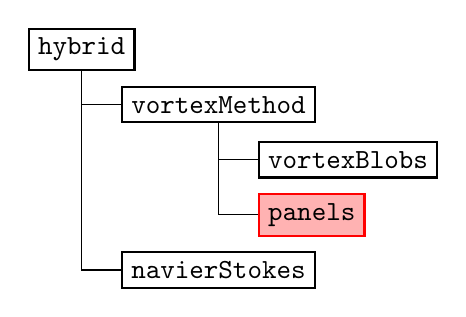
\begin{tikzpicture}[%
  grow via three points={one child at (0.5,-0.7) and
  two children at (0.5,-0.7) and (0.5,-1.4)},
  edge from parent path={(\tikzparentnode.south) |- (\tikzchildnode.west)}]
  \node {\texttt{hybrid}}
    child { node {\texttt{vortexMethod}}
    	child {node {\texttt{vortexBlobs}}}
    	child {node [selected] {\texttt{panels}}}  	
    }
    child [missing] {}				
    child [missing] {}				
    child { node {\texttt{navierStokes}}};
    %child { node [selected] {tex}
    %  child { node {generic}}
    %  child { node [optional] {latex}}
    %  child { node {plain}}
    %}
    %child [missing] {}
    %child { node {texdoc}};
\end{tikzpicture}
\end{figure}


\subsection*{Class structure:}
\begin{figure}[h]
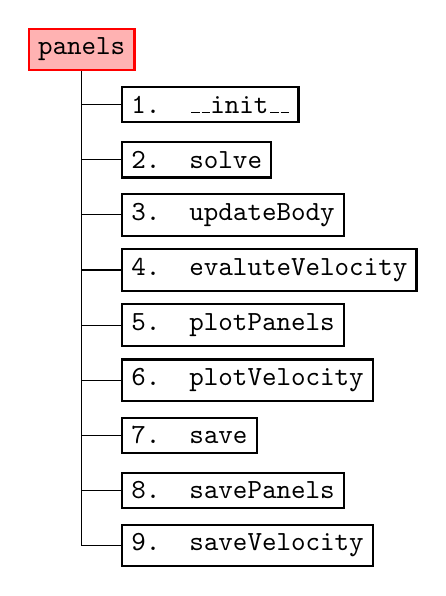
\begin{tikzpicture}[%
  grow via three points={one child at (0.5,-0.7) and
  two children at (0.5,-0.7) and (0.5,-1.4)},
  edge from parent path={(\tikzparentnode.south) |- (\tikzchildnode.west)}]
  \node [selected] {\texttt{panels}}
    child { node {\texttt{1. \_\_init\_\_}}}
    child { node {\texttt{2. solve}}}
    child { node {\texttt{3. updateBody}}}    
    child { node {\texttt{4. evaluteVelocity}}}                    
    child { node {\texttt{5. plotPanels}}}                        
    child { node {\texttt{6. plotVelocity}}}                        
    child { node {\texttt{7. save}}}                        
    child { node {\texttt{8. savePanels}}}                                        
    child { node {\texttt{9. saveVelocity}}};                                            
	%  child { node [selected] {tex}
    %  child { node {generic}}
    %  child { node [optional] {latex}}
    %  child { node {plain}}
    %}
    %child { node {texdoc}};
\end{tikzpicture}
\end{figure}

\subsection{\texttt{\_\_init\_\_}}
	\begin{tabular}{l|lp{7cm}}
		\multicolumn{2}{l}{\textbf{Input Parameters}} & \\ \hline
		\textit{File Name} & \multicolumn{2}{l}{Containing all the parameters to re-initalize the class.} \\ \hline
		\multirow{2}{*}{\textit{Parameters}} & Panel coordinates &: \{\texttt{xCP, yCP, xPanel, yPanel, cmGlobal, thetaLocal}\}\\ \cline{2-3}
		& External velocity &: \texttt{externVel} \\ \cline{2-3}
	\end{tabular}
	\paragraph{Description:} Initialize the \texttt{panels} class with the given input parameters. In the case of a multibody problem, a list of panel coordinates can be given and internally it takes care of the inter-coupling.\\
	\\
	\begin{tabular}{lp{10cm}}
				\textit{Panel coordinates} & \\ \hline
				\texttt{xCP,yCP} &:  the local $x,y$-coordinates of the panel collocation points.\\ 
				\texttt{xPanel,yPanel} &: the local coordinate of the panel edges. \textit{Note}: Should have a closed loop (end with initial point coordinates).\\ 
				\texttt{cmGlobal} &:  the position of reference points of a given panel body.\\
				\texttt{thetaLocal} &:  the rotational angles of the panel body axes w.r.t to the global $x$-axis.\\
	\end{tabular}\\ 
    \\ \\
	\begin{tabular}{lp{10cm}}
				\textit{External velocity} & \\ \hline
				\texttt{externVel} &:  Reference to an external velocity \textbf{function} acting of the panels. For the panel case, the external velocity will the induced velocity of the blobs + freestream \texttt{vortexBlob.evaluateVelocity}.\\
	\end{tabular}\\
	
		\begin{tabular}{lp{10cm}}
			\textbf{Input parameters} &: \texttt{xCP,yCP}\\ 
			\textbf{Assigns} &: \texttt{-}\\ 			
			\textbf{Returns} &: \texttt{vxCP,vyCP}\\ 					
		\end{tabular}\\

		
\subsection{\texttt{solve}}
	\paragraph{Description:} Function to solve the panel strength to satisfy no-slip condition.\\
	
		\begin{tabular}{lp{10cm}}
			\textit{Parameters} & \\ \hline
			\texttt{sPanel} &: the new strength of the panels, satisfying the no-through b.c of the body (no-slip with vortex panels.).\\
		\end{tabular} \vspace{5 mm}
		\\		
		\begin{tabular}{lp{10cm}}
			\textbf{Input parameters} &: \texttt{-}\\ 
			\textbf{Assigns} &: \texttt{sPanel}\\ 			
			\textbf{Returns} &: \texttt{-}\\ 					
		\end{tabular}		
			
		
\subsection{\texttt{updateBody}}
	\paragraph{Description:} Function to update all the panel body coordinates. This function will internally calculate the new panel coordinates \texttt{xPanel,yPanel,xCP,yCP} and rebuild the inter-induction matrix \texttt{A}.\\
	
		\begin{tabular}{lp{10cm}}
			\textit{Parameters} & \\ \hline
			\texttt{xPanel,yPanel} &: the $x,y$ panel coordinates in global.\\
			\texttt{xCP,yCP} &: the $x,y$ coordinates of the collocation point in global.\\
			\texttt{A} &: the panel self-induction matrix.
		\end{tabular} \vspace{5 mm}
		\\		
		\begin{tabular}{lp{10cm}}
			\textbf{Input parameters} &: \texttt{thetaLocals,cmGlobals}\\ 
			\textbf{Assigns} &: \texttt{A, xPanel, yPanel, xCP, yCP}\\ 			
			\textbf{Returns} &: \texttt{-}\\ 					
		\end{tabular}	

\subsection{\texttt{evaluateVelocity}}
	\paragraph{Description:} Function to evaluate the total induced velocity due to the panels and free-stream velocity (\textit{optional}).\\
	
	    \begin{tabular}{lp{10cm}}
			\textit{Parameters} & \\ \hline
			 \texttt{xTarget,yTarget} &: the $x,y$ coordinate of the target location, where the total velocity is to be evaluated.\\
			\texttt{vxTarget,vyTarget} &: the $x,y$ induced velocity of the target points in global coordinate system.\\
		\end{tabular} \vspace{5 mm}
	\\		
	\begin{tabular}{lp{10cm}}
		\textbf{Input parameters} &: \texttt{xTarget,yTarget}\\ 
		\textbf{Assigns} &: \texttt{-}\\ 			
		\textbf{Returns} &: \texttt{vxTarget,vyTarget}\\ 					
	\end{tabular}					

		
\subsection{plots \ldots}
	\paragraph{Description:} Function to plot and save (\textit{optional}) all the results in a given region or set of points.\\
	
		\begin{tabular}{lp{10cm}}
			\textit{Plot variables:} & \\ \hline
			\texttt{plotPanels} &:plot the panel coordinates at the current time instant.\\
			\texttt{plotVelocity} &: plot the velocity field.\\ 
			\texttt{plotVorticity} &: plot the vorticity field.\\ 
		\end{tabular} \vspace{5 mm}
		
		\begin{tabular}{lp{10cm}}
			\textit{Parameters:} & \\ \hline
			\texttt{xBounds,yBounds} &: $x,y$ bounds of the grid, where the data is to be evaluated and saved.\\ 
			\texttt{nGrid} &: $x,y$ number of evaluation grid points.\\ 
			\texttt{xEval,yEval} &: $x,y$ coordinates of the location where the data is to be evaluated and saved.\\ 
		\end{tabular} \vspace{5 mm}\\
	\\
	\begin{tabular}{lp{10cm}}
		\textbf{Input parameters} &: \texttt{xBounds,yBounds,hGrid} or \texttt{xEval,yEval}\\ 
		\textbf{Assigns} &: \texttt{-}\\ 			
		\textbf{Returns} &: \texttt{figureHandle} and/or \texttt{.pvd}\\ 					
	\end{tabular}	

\subsection{save data \ldots}
	\paragraph{Description:} Function to save the data in a given region or at given set of points.\\

		\begin{tabular}{lp{10cm}}
			\textit{Save variables:} & \\ \hline
			\texttt{save} &: all the data of the \texttt{panels} class, to be used to restart later.\\ 			
			\texttt{savePanels} &: the function to save the panel data at the current time instant.\\ 			
			\texttt{saveVelocity} &: save the velocity field of the given region or the given set of points.\\ 
			\texttt{saveVorticity} &: save the vorticity field of the given region or the given set of points.\\ 
		\end{tabular} \vspace{5 mm}
	
		\begin{tabular}{lp{10cm}}
			\textit{Parameters:} & \\ \hline
			\texttt{xBounds,yBounds} &: $x,y$ bounds of the grid, where the data is to be evaluated and saved.\\ 
			\texttt{nGrid} &: $x,y$ number of grid points.\\ 
			\texttt{xEval,yEval} &: $x,y$ coordinates of the location where the data is the be evaluated and saved.\\ 
		\end{tabular} \vspace{5 mm}\\
	\\
	\begin{tabular}{lp{10cm}}
		\textbf{Input parameters} &: \texttt{xBounds,yBounds,hGrid} or \texttt{xEval,yEval}\\ 
		\textbf{Assigns} &: \texttt{-}\\ 			
		\textbf{Returns} &: \texttt{.npz}\\ 					
	\end{tabular}

%
%
%\subsection{save plots \ldots}
%	\paragraph{Description:} Function to save the plots of a region or a given set of points as scientific visualization format \texttt{.pvd}.\\
%	
%		\begin{tabular}{lp{10cm}}
%			\textit{Save variables:} & \\ \hline
%			\texttt{saveVelocityPlot} &: save the velocity $\mathbf{V}$ plot.\\ 
%			\texttt{saveVorticityPlot} &: save the vorticity $\mathbf{\omega}$ plot.\\ 
%		\end{tabular} \vspace{5 mm}
%		
%		\begin{tabular}{lp{10cm}}
%			\textit{Parameters:} & \\ \hline
%			\texttt{xBounds,yBounds} &: $x,y$ bounds of the grid, where the data is to be evaluated and saved.\\ 
%			\texttt{hGrid} &: $x,y$ spacing of the evaluation grid.\\ 
%			\texttt{xEval,yEval} &: $x,y$ coordinates of the location where the data is the be evaluated and saved.\\ 
%		\end{tabular} \vspace{5 mm}\\
%	\\
%	\begin{tabular}{lp{10cm}}
%		\textbf{Input parameters} &: \texttt{xBounds,yBounds,hGrid} or \texttt{xEval,yEval} \\ 
%		\textbf{Assigns} &: \texttt{-}\\ 			
%		\textbf{Returns} &: \texttt{.pvd}\\ 					
%	\end{tabular}
%\section{\texttt{vortexMethod}}
The main structure of the \texttt{vortexBlobs} + \texttt{panels} (vortexMethod) class. This class contains all the function related to the calculations of panel with vortex blobs.

\begin{figure}[h]
\centering
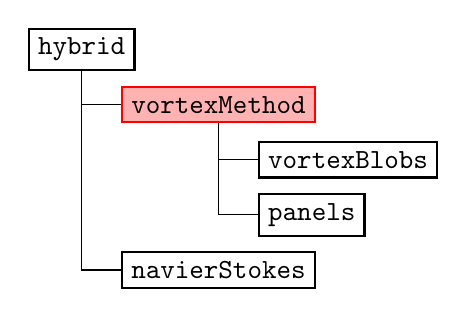
\begin{tikzpicture}[%
  grow via three points={one child at (0.5,-0.7) and
  two children at (0.5,-0.7) and (0.5,-1.4)},
  edge from parent path={(\tikzparentnode.south) |- (\tikzchildnode.west)}]
  \node {\texttt{hybrid}}
    child { node [selected] {\texttt{vortexMethod}}
    	child {node {\texttt{vortexBlobs}}}
    	child {node {\texttt{panels}}}  	
    }
    child [missing] {}				
    child [missing] {}				
    child { node {\texttt{navierStokes}}};
    %child { node [selected] {tex}
    %  child { node {generic}}
    %  child { node [optional] {latex}}
    %  child { node {plain}}
    %}
    %child [missing] {}
    %child { node {texdoc}};
\end{tikzpicture}
\end{figure}

\subsection*{Class structure:}
\begin{figure}[h]
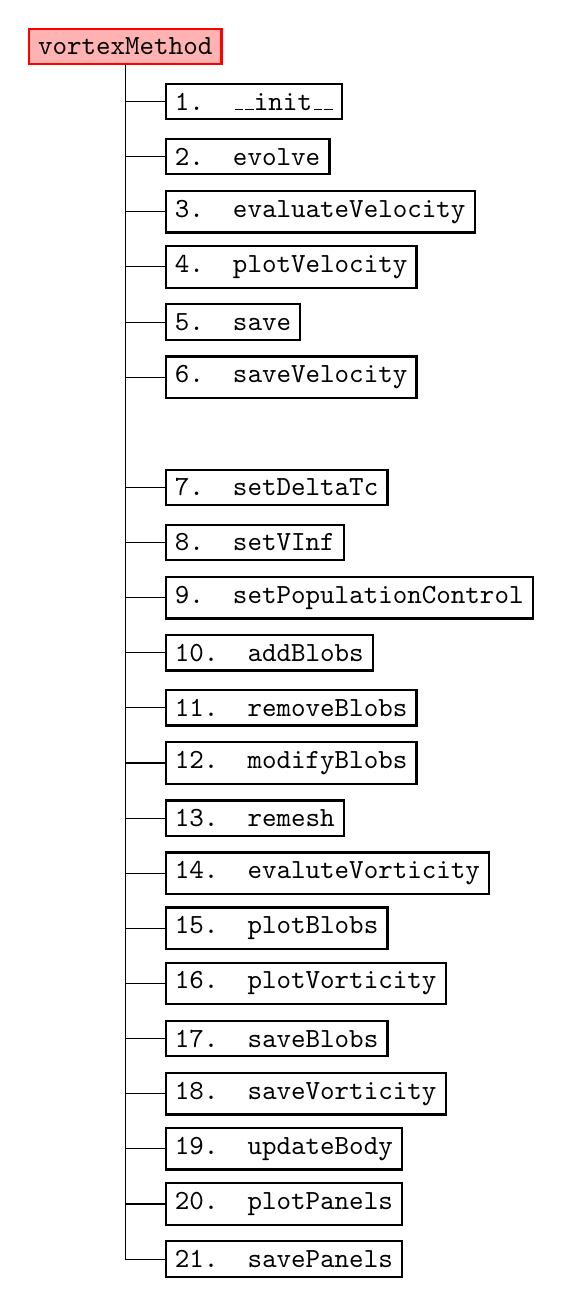
\begin{tikzpicture}[%
  grow via three points={one child at (0.5,-0.7) and
  two children at (0.5,-0.7) and (0.5,-1.4)},
  edge from parent path={(\tikzparentnode.south) |- (\tikzchildnode.west)}]
  \node [selected] {\texttt{vortexMethod}}
    child { node {\texttt{1. \_\_init\_\_}}}
    child { node {\texttt{2. evolve}}}
    child { node {\texttt{3. evaluateVelocity}}}
    child { node {\texttt{4. plotVelocity}}}                        
    child { node {\texttt{5. save}}}                        
    child { node {\texttt{6. saveVelocity}}}                                            
    child [missing] {}
    child { node {\texttt{7. setDeltaTc}}}
    child { node {\texttt{8. setVInf}}}    
    child { node {\texttt{9. setPopulationControl}}}
    child { node {\texttt{10. addBlobs}}}
    child { node {\texttt{11. removeBlobs}}}    
    child { node {\texttt{12. modifyBlobs}}}    
    child { node {\texttt{13. remesh}}}    
    child { node {\texttt{14. evaluteVorticity}}}                        
    child { node {\texttt{15. plotBlobs}}}                        
    child { node {\texttt{16. plotVorticity}}}                            
    child { node {\texttt{17. saveBlobs}}}                                        
    child { node {\texttt{18. saveVorticity}}}
    child { node {\texttt{19. updateBody}}}    
    child { node {\texttt{20. plotPanels}}}                        
    child { node {\texttt{21. savePanels}}};                                        
    	             
%    child { node {\texttt{5. plotPanels}}}                        
%    child { node {\texttt{6. plotVelocity}}}                        
%    child { node {\texttt{7. save}}}                        
%    child { node {\texttt{8. savePanels}}}                                        
%    child { node {\texttt{9. saveVelocity}}};                                            
	%  child { node [selected] {tex}
    %  child { node {generic}}
    %  child { node [optional] {latex}}
    %  child { node {plain}}
    %}
    %child { node {texdoc}};
\end{tikzpicture}
\end{figure}

%
%
%\subsection*{Class structure:}
%\begin{table}[h]
%\begin{tabular}{rl}
%	\texttt{vortexMethod}: &  \\ \hline
%	-- & \texttt{\_\_init\_\_} \\
%	& \\
%	-- & \texttt{evolve} \\ 
%	-- & \texttt{evaluateVelocity} \\ 
%	-- & \texttt{plotBlobsPanels} \\ 	
%	-- & \texttt{plotVelocity} \\ 
%	-- & \texttt{plotVorticity} \\ 	
%	-- & \texttt{saveClass} \\ 
%	-- & \texttt{saveVelocity} \\ 
%	-- & \texttt{saveVorticity} \\ 
%	-- & \texttt{saveVelocityPlot} \\ 
%	-- & \texttt{saveVorticityPlot} \\ 	
%\end{tabular}
%%\caption{\texttt{vortexMethod} class structure}
%\end{table}

\subsection{\texttt{\_\_init\_\_}}
	\begin{tabular}{l|lp{7cm}}
		\multicolumn{2}{l}{\textbf{Input Parameters}} & \\ \hline
		\textit{File Name} & \multicolumn{2}{l}{Containing all the parameters to re-initalize the class.} \\ \hline
		\multirow{2}{*}{\textit{Parameters}} & \texttt{vortexBlobs} &: \{\texttt{vortexBlobs}\} class. \\ \cline{2-3}
		& \texttt{panels} &: \texttt{panels} class. \\ \cline{2-3}
	\end{tabular}
	\paragraph{Description:} Initialize the \texttt{vortexMethod} class using \textbf{vortexBlob}+\textbf{panelMethod} classes.
	\paragraph{Input parameters:}
	\begin{list}{\quad}{}
	\item \texttt{vortexBlob}: vortex particle class
	\item \texttt{panelMethod}: panel method class				
	\end{list}

\subsection{\texttt{evolve}}
	\paragraph{Description:} Function to evolve (i.e. step) the vortex and panel together. All the necessary parameters are preassigned during the init of the vortex and panel class.\\
	
	    \begin{tabular}{lp{10cm}}
			\textit{Parameters:} & \\ \hline
			 \texttt{xBlobNew,yBlobNew,gBlobNew} &: the new $x,y$ coordinate and the new circulation $\Gamma_i$ of the blob at the new time instant.\\
			\texttt{xPanelNew,yPanelNew,sPanelNew} &: the new $x,y$ coordinates of the panel and its new strength at the new time instant.\\
		\end{tabular} \vspace{5 mm}
	\\		
	\begin{tabular}{lp{10cm}}
		\textbf{Input parameters} &: \texttt{-}\\ 
		\textbf{Assigns} &: \texttt{xBlob,yBlob,gBlob,xPanel,yPanel,sPanel}\\ 			
		\textbf{Returns} &: \texttt{-}\\ 					
	\end{tabular}

\subsection{\texttt{evaluateVelocity}}
	\paragraph{Description:} Function to evaluate the total induced velocity due to the vortex blobs, panels, and the external velocity at a given target coordinates.\\
	
	    \begin{tabular}{lp{10cm}}
			\textit{Parameters} & \\ \hline
			 \texttt{xTarget,yTarget} &: the $x,y$ coordinate of the target location, where the total velocity is to be evaluated.\\
			\texttt{vxTarget,vyTarget} &: the $x,y$ induced velocity of the target points in global coordinate system.\\
		\end{tabular} \vspace{5 mm}
	\\		
	\begin{tabular}{lp{10cm}}
		\textbf{Input parameters} &: \texttt{xTarget,yTarget}\\ 
		\textbf{Assigns} &: \texttt{-}\\ 			
		\textbf{Returns} &: \texttt{vxTarget,vyTarget}\\ 					
	\end{tabular}
		
\subsection{plots \ldots}
	\paragraph{Description:} Function to plot and save (\textit{optional}) all the results in a given region or set of points.\\
	
		\begin{tabular}{lp{10cm}}
			\textit{Plot variables:} & \\ \hline
			\texttt{plotBlobs/plotPanels} &: the plot of blobs and the panel coordinates.\\
			\texttt{plotVelocity} &: plot the velocity field of the region of the given set of points.\\ 
			\texttt{plotVorticity} &: plot the vorticity field.\\ 
		\end{tabular} \vspace{5 mm}
		
		\begin{tabular}{lp{10cm}}
			\textit{Parameters:} & \\ \hline
			\texttt{xBounds,yBounds} &: $x,y$ bounds of the grid, where the data is to be evaluated and saved.\\ 
			\texttt{nGrid} &: $x,y$ number of grid points.\\ 
			\texttt{xEval,yEval} &: $x,y$ coordinates of the location where the data is the be evaluated and saved.\\ 
		\end{tabular} \vspace{5 mm}\\
	\\
	\begin{tabular}{lp{10cm}}
		\textbf{Input parameters} &: \texttt{xBounds,yBounds,nGrid} or \texttt{xEval,yEval}\\ 
		\textbf{Assigns} &: \texttt{-}\\ 			
		\textbf{Returns} &: \texttt{figureHandle} or \texttt{saveFile}\\ 					
	\end{tabular}						

\subsection{save data \ldots}
	\paragraph{Description:} Function to save the data in a given region or at given set of points.\\

		\begin{tabular}{lp{10cm}}
			\textit{Save variables:} & \\ \hline
			\texttt{save} &: all the data of the \texttt{vortexMethod} class, to be used to restart later.\\ 			
			\texttt{saveBlobs/savePanels} &: the function to save the blobs and panel data at the current time instant.\\ 			
			\texttt{saveVelocity} &: the velocity field.\\ 
			\texttt{saveVorticity} &: the vorticity field.\\ 
		\end{tabular} \vspace{5 mm}
	
		\begin{tabular}{lp{10cm}}
			\textit{Parameters:} & \\ \hline
			\texttt{xBounds,yBounds} &: $x,y$ bounds of the grid, where the data is to be evaluated and saved.\\ 
			\texttt{nGrid} &: $x,y$ number of grid points.\\ 
			\texttt{xEval,yEval} &: $x,y$ coordinates of the location where the data is the be evaluated and saved.\\ 
		\end{tabular} \vspace{5 mm}\\
	\\
	\begin{tabular}{lp{10cm}}
		\textbf{Input parameters} &: \texttt{xBounds,yBounds,nGrid} or \texttt{xEval,yEval}\\ 
		\textbf{Assigns} &: \texttt{-}\\ 			
		\textbf{Returns} &: \texttt{.npz}\\ 					
	\end{tabular}

%\subsection{save plots \ldots}
%	\paragraph{Description:} Function to save the plots of a region or a given set of points as scientific visualization format \texttt{.pvd}.\\
%	
%		\begin{tabular}{lp{10cm}}
%			\textit{Save variables:} & \\ \hline
%			\texttt{saveVelocityPlot} &: save the velocity $\mathbf{V}$ plot.\\ 
%			\texttt{saveVorticityPlot} &: save the vorticity $\mathbf{\omega}$ plot.\\ 
%		\end{tabular} \vspace{5 mm}
%		
%		\begin{tabular}{lp{10cm}}
%			\textit{Parameters:} & \\ \hline
%			\texttt{xBounds,yBounds} &: $x,y$ bounds of the grid, where the data is to be evaluated and saved.\\ 
%			\texttt{hGrid} &: $x,y$ spacing of the evaluation grid.\\ 
%			\texttt{xEval,yEval} &: $x,y$ coordinates of the location where the data is the be evaluated and saved.\\ 
%		\end{tabular} \vspace{5 mm}\\
%	\\
%	\begin{tabular}{lp{10cm}}
%		\textbf{Input parameters} &: \texttt{xBounds,yBounds,hGrid} or \texttt{xEval,yEval} \\ 
%		\textbf{Assigns} &: \texttt{-}\\ 			
%		\textbf{Returns} &: \texttt{.pvd}\\ 					
%	\end{tabular}
%\section{\texttt{navierStokes}}
The main structure for the Navier-stokes class \texttt{navierStokes}. This class contains all the functions related to computation of the Navier-stokes problem. Below is set of functions that acts as the interface to the class.

\begin{figure}[h]
\centering
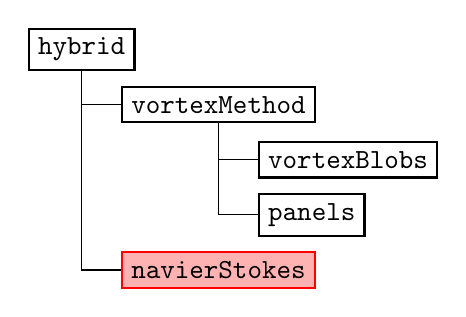
\begin{tikzpicture}[%
  grow via three points={one child at (0.5,-0.7) and
  two children at (0.5,-0.7) and (0.5,-1.4)},
  edge from parent path={(\tikzparentnode.south) |- (\tikzchildnode.west)}]
  \node {\texttt{hybrid}}
    child { node {\texttt{vortexMethod}}
    	child {node {\texttt{vortexBlobs}}}
    	child {node {\texttt{panels}}}  	
    }
    child [missing] {}				
    child [missing] {}				
    child { node [selected] {\texttt{navierStokes}}};
    %child { node [selected] {tex}
    %  child { node {generic}}
    %  child { node [optional] {latex}}
    %  child { node {plain}}
    %}
    %child [missing] {}
    %child { node {texdoc}};
\end{tikzpicture}
\end{figure}


\subsection*{Class structure:}
\begin{figure}[h]
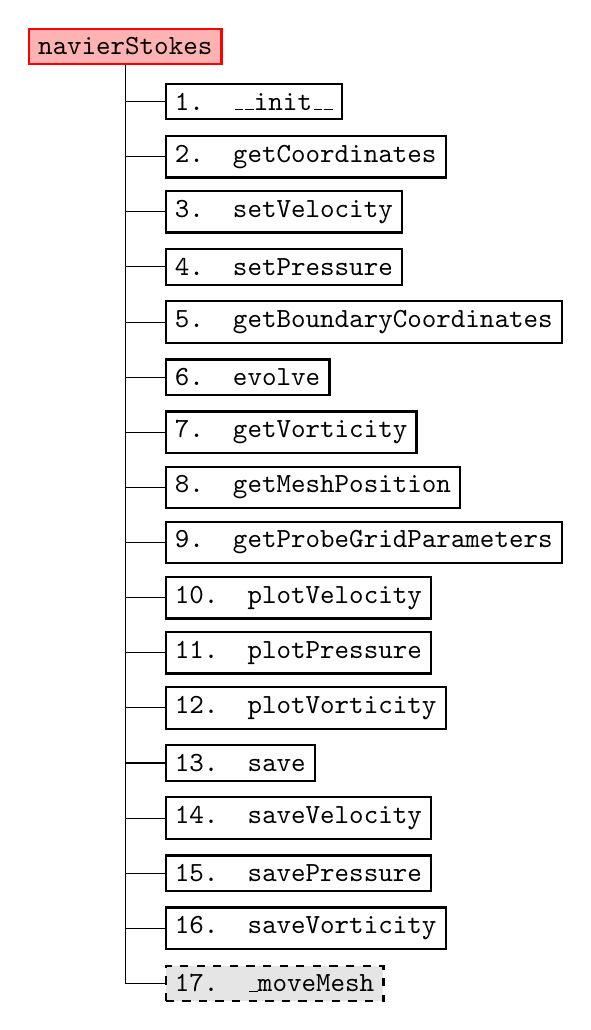
\begin{tikzpicture}[%
  grow via three points={one child at (0.5,-0.7) and
  two children at (0.5,-0.7) and (0.5,-1.4)},
  edge from parent path={(\tikzparentnode.south) |- (\tikzchildnode.west)}]
  \node [selected] {\texttt{navierStokes}}
    child { node {\texttt{1. \_\_init\_\_}}}
    child {node  {\texttt{2. getCoordinates}}}
    child { node {\texttt{3. setVelocity}}}
    child { node {\texttt{4. setPressure}}}
    child { node {\texttt{5. getBoundaryCoordinates}}}                        
    child { node {\texttt{6. evolve}}}
    child { node {\texttt{7. getVorticity}}}                        
    child { node {\texttt{8. getMeshPosition}}}                        
    child { node {\texttt{9. getProbeGridParameters}}}                        
    child { node {\texttt{10. plotVelocity}}}                        
    child { node {\texttt{11. plotPressure}}}                        
    child { node {\texttt{12. plotVorticity}}}                        
    child { node {\texttt{13. save}}}                        
    child { node {\texttt{14. saveVelocity}}}                                            
    child { node {\texttt{15. savePressure}}}                                            
    child { node {\texttt{16. saveVorticity}}}
    child { node [optional]{\texttt{17. \_moveMesh}}};
	%  child { node [selected] {tex}
    %  child { node {generic}}
    %  child { node [optional] {latex}}
    %  child { node {plain}}
    %}
    %child { node {texdoc}};
\end{tikzpicture}
\end{figure}

%\subsection*{Class structure:}
%\begin{table}[h]
%\begin{tabular}{rl}
%	\texttt{navierStokes}: &  \\ \hline
%	-- & \texttt{\_\_init\_\_} \\
%	& \\
%	-- & \texttt{initialConditions} \\ 
%	-- & \texttt{evolve} \\ 
%	-- & \texttt{boundaryCoordinates} \\ 
%	-- & \texttt{updateMesh} \\ 
%	-- & \texttt{moveMesh} \\ 
%	-- & \texttt{computeVorticity} \\ 
%	-- & \texttt{meshPosition}\\
%	-- & \texttt{probeGridParameters} \\ 	
%	-- & \texttt{plotVelocity} \\ 		
%	-- & \texttt{plotPressure} \\ 		
%	-- & \texttt{plotVorticity} \\ 			
%	-- & \texttt{saveClass} \\ 					
%	-- & \texttt{saveVelocity} \\ 		
%	-- & \texttt{savePressure} \\ 		
%	-- & \texttt{saveVorticity} \\ 	
%	-- & \texttt{saveVelocityPlot} \\ 		
%	-- & \texttt{savePressurePlot} \\ 		
%	-- & \texttt{saveVorticityPlot} \\ 	
%\end{tabular}
%%\caption{\texttt{navierStokes} class structure}
%\end{table}

\newpage

\subsection{\texttt{\_\_init\_\_}}
	\paragraph{Description:} Initialize the \texttt{navierStokes} class either using a \texttt{fileName} containing all the necessary parameter for initialization or by explicitly inputing the parameters.\\

	\begin{tabular}{l|lp{7cm}}
		\multicolumn{2}{l}{\textbf{Input Parameters}} & \\ \hline
		\textit{File Name} & \multicolumn{2}{l}{Containing all the parameters to re-initalize the class.} \\ \hline
		\multicolumn{3}{c}{-- or --} \\ \hline
		\multirow{5}{*}{\textit{Parameters}} & Mesh data &: \texttt{mesh, boundaryDomains}\\ \cline{2-3}
		& Geometry position &: \texttt{cmGlobal, thetaLocal} \\ \cline{2-3}
		& Fluid parameters &: \texttt{uMax, nu}\\ \cline{2-3}
		& Solver options &: \texttt{cfl}\\ \cline{2-3}
		& Probe grid parameters &: \texttt{x0, y0, Lx, Ly, hx, hy}\\ \cline{2-3}

	\end{tabular}\\
	\subsubsection*{Descrition of the parameters:}
	
	\begin{tabular}{lp{10cm}}
				\textit{Mesh data} & \\ \hline
				\texttt{mesh} &: the mesh data file.\\ 
				\texttt{boundaryDomains} &: the boundary mesh domain data file.\\ 			
	\end{tabular}\\ 
    \\ \\
	\begin{tabular}{lp{10cm}}
				\textit{Geometry position} & \\ \hline
				\texttt{cmGlobal} &: the $x,y$ position of the geometry in global coordinates.\\ 
				\texttt{thetaGlobal} &: the rotation angle (in $rad$) of the geometry in global coordinate system.\\ 			
	\end{tabular}\\
    \\ \\
	\begin{tabular}{lp{10cm}}
				\textit{Fluid parameters} & \\ \hline
				\texttt{uMax} &: the maximum fluid velocity $U_{max}$. Used to determine the maximum time step size $\Delta t_{max}$.\\ 
				\texttt{nu} &: the fluid kinematic viscosity $\nu$, for incompressible navier-stokes problem.\\ 			
	\end{tabular}\\	
    \\ \\
	\begin{tabular}{lp{10cm}}
				\textit{Solver options} & \\ \hline
				\texttt{cfl} &: the $CFL$ stability parameter. If explicit time marching scheme, $CFL<1$.\\ 		
	\end{tabular}\\	
    \\ \\
	\begin{tabular}{lp{10cm}}
				\textit{Probe grid parameters} & \\ \hline
				\texttt{x0,y0} &: the $x,y$ coordinate of the origin of the probe grid.\\ 
				\texttt{Lx,Ly} &: the $x,y$ size (width and height) of the probing grid.\\ 			
				\texttt{hx,hy} &: the $x,y$ spacing of the probe grid cell.\\ 							
	\end{tabular}\\	

\subsection{\texttt{getCoordinates}}
	\paragraph{Description:} Function to get all the coordinates of the velocity function spaces $\mathbf{V}$. With the returned coordinates, one could calculate the velocity field in the navier-stokes domain. \textit{Note}: The coordinates and just a list of DOF coordinate of the vector function space and is given in the same order as the data that is to be stored.\\
	
	    \begin{tabular}{lp{10cm}}
			\textit{Parameters} & \\ \hline
			\texttt{xCoordinates,yCoordinates} &: the $x,y$ coordinates of the velocity vector function space $\mathbf{V}$. \\		
		\end{tabular} \vspace{5 mm}
	\\		
	\begin{tabular}{lp{10cm}}
		\textbf{Input parameters} &: \texttt{-}\\ 
		\textbf{Assigns} &: \texttt{-}\\ 			
		\textbf{Returns} &: \texttt{xCoordinates,yCoordinates}\\ 					
	\end{tabular}

\subsection{\texttt{setVelocity}}
	\paragraph{Description:} Function to apply the current velocity field.\\
	
	    \begin{tabular}{lp{10cm}}
			\textit{Parameters} & \\ \hline
			\texttt{vFieldNew} &: the \textit{new} velocity at the navier-stokes DOF coordinates of the vector function space $\mathbf{V}$.\\		
		\end{tabular} \vspace{5 mm}
	\\		
	\begin{tabular}{lp{10cm}}
		\textbf{Input parameters} &: \texttt{vFieldNew}\\ 
		\textbf{Assigns} &: \texttt{vField}\\ 			
		\textbf{Returns} &: \texttt{-}\\ 					
	\end{tabular}
	
\subsection{\texttt{setPressure}}
	\paragraph{Description:} Function to apply the current pressure field.\\
	
	    \begin{tabular}{lp{10cm}}
			\textit{Parameters} & \\ \hline
			\texttt{pFieldNew} &: the \textit{new} pressure field at the navier-stokes DOF coordinates of the scalar function space $\mathbf{V}$.\\ 
		\end{tabular} \vspace{5 mm}
	\\		
	\begin{tabular}{lp{10cm}}
		\textbf{Input parameters} &: \texttt{pFieldNew}\\ 
		\textbf{Assigns} &: \texttt{pField}\\ 			
		\textbf{Returns} &: \texttt{-}\\ 					
	\end{tabular}

\subsection{\texttt{getBoundaryCoordinates}}
	\paragraph{Description:} Function to return the boundary DOF coordinates \texttt{xBoundary,yBoundary} of the vector function space $\mathbf{V}$.\\
	
		\begin{tabular}{lp{10cm}}
			\textit{Parameters} & \\ \hline
			\texttt{xBoundary,yBoundary} &: $x,y$ boundary coordinates of the vector function space  $\mathbf{V}$. \\ 
		\end{tabular} \vspace{5 mm}
	\\
	\begin{tabular}{lp{10cm}}
		\textbf{Input parameters} &: \texttt{-}\\ 
		\textbf{Assigns} &: \texttt{-}\\ 			
		\textbf{Returns} &: \texttt{xBoundary,yBoundary}\\ 					
	\end{tabular}	

\subsection{\texttt{evolve}}
	\paragraph{Description}: Function to evolve the Navier-stokes by one step with the $x,y$ velocity boundary condition \texttt{vxBoundary,vyBoundary} at the Navier-stokes finite element mesh boundary \texttt{xBoundary,yBoundary}. The function will calculate the new velocity and the pressure fields. The \textit{new} mesh position is used to update the mesh position, whereas the \textit{current} mesh velocity is used to calculate the modified convective term to take in account of the rigid mesh motion.\\
	
		\begin{tabular}{lp{10cm}}
			\textit{Parameters} & \\ \hline
			\texttt{vxBoundary,vyBoundary} &: $x,y$ velocity at the navier-stokes dof boundary coordinates as described by \texttt{xBoundary,yBoundary}.\\ 
			\texttt{xBoundary,yBoundary} &: $x,y$ boundary coordinates of the vector function space.\\ 
			\texttt{cmGlobalNew,thetaGlobalNew} &: the \textit{new} mesh position and the global mesh rotational angle\\
			\texttt{cmDotGlobal, thetaDotGlobal} &: the \textit{current} mesh velocities (displacement velocity and rotational velocity) in the global reference frame.\\
		\end{tabular} \vspace{5 mm}
	\\	
	\begin{tabular}{lp{10cm}}
		\textbf{Input parameters} &: \texttt{vxBoundary,vyBoundary, cmGlobalNew,thetaGlobalNew, cmDotGlobal, thetaDotGlobal}\\ 
		\textbf{Assigns} &: \texttt{vField, pField}\\ 			
		\textbf{Returns} &: \texttt{-}\\ 					
	\end{tabular}	


	

%
%\subsection{\texttt{moveMesh}}
%	\paragraph{Description:} Function to move the mesh using body displacement and rotational velocities. This function can be then used to calculate the mesh velocity of the current instant.\\
%	
%		\begin{tabular}{lp{10cm}}
%			\textit{Parameters} & \\ \hline
%			\texttt{cmDotGlobal} &: the $x,y$ global mesh coordinate displacement velocity.\\ 
%			\texttt{thetaDotGlobal} &: the polar rotational velocity of the navier-stokes domain w.r.t global coordintes.\\ 			
%			\texttt{vMesh} &: the mesh velocity w.r.t to global $x,y$-axis\\	
%		\end{tabular} \vspace{5 mm}
%	\\
%	\begin{tabular}{lp{10cm}}
%		\textbf{Input parameters} &: \texttt{cmDotGlobal,thetaDotGlobal}\\ 
%		\textbf{Assigns} &: \texttt{xBoundary,yBoundary,vMesh}\\ 			
%		\textbf{Returns} &: \texttt{-}\\ 					
%	\end{tabular}
	
	
\subsection{\texttt{getVorticity}}
	\paragraph{Description:} Function to evaluate the vorticity at probe coordinates defined by the probe mesh.\\
	
		\begin{tabular}{lp{10cm}}
			\textit{Parameters} & \\ \hline
			\texttt{vortProbeGrid} &: the vorticity $\omega$ at the probe grid coordinates \texttt{xProbeGrid, yProbeGrid}.\\ 
		\end{tabular} \vspace{5 mm}
	\\
	\begin{tabular}{lp{10cm}}
		\textbf{Input parameters} &: \texttt{-}\\ 
		\textbf{Assigns} &: \texttt{-}\\ 			
		\textbf{Returns} &: \texttt{wProbeGrid}\\ 					
	\end{tabular}


\subsection{\texttt{getMeshPosition}}

	\paragraph{Description:} Function to return the current mesh position and rotational angle.\\
	
		\begin{tabular}{lp{10cm}}
			\textit{Parameters} & \\ \hline
			\texttt{cmGlobal} &: the $x,y$ position of the mesh in global coordinates.\\ 
			\texttt{thetaGlobal} &: the rotational angle of the mesh w.r.t the global $x$ axis.\\
		\end{tabular} \vspace{5 mm}
	\\
	\begin{tabular}{lp{10cm}}
		\textbf{Input parameters} &: \texttt{-}\\ 
		\textbf{Assigns} &: \texttt{-}\\ 			
		\textbf{Returns} &: \texttt{cmGlobal,thetaGlobal}\\ 					
	\end{tabular}

\subsection{\texttt{getProbeGridParameters}}

	\paragraph{Description:} Function to return the probe grid parameters.\\
	
		\begin{tabular}{lp{10cm}}
			\textit{Parameters} & \\ \hline
			\texttt{x0,y0} &: the global $x,y$ coordinates of the probe mesh origin.\\ 
			\texttt{Lx,Ly} &: the local width and height of the probe mesh.\\
			\texttt{hx,hy} &: the probe spacing of the structure probe mesh.\\			
		\end{tabular} \vspace{5 mm}
	\\
	\begin{tabular}{lp{10cm}}
		\textbf{Input parameters} &: \texttt{-}\\ 
		\textbf{Assigns} &: \texttt{-}\\ 			
		\textbf{Returns} &: \texttt{x0,y0,Lx,Ly,hx,hy}\\ 					
	\end{tabular}

\subsection{plots \ldots}
	\paragraph{Description:} Function to plot and/or save (\textit{optional}) all the results.\\
	
		\begin{tabular}{lp{10cm}}
			\textit{Plot variables} & \\ \hline
			\texttt{plotVelocity} &: the velocity $\mathbf{V}$ of the navier-stokes domain, \texttt{u1}.\\ 
			\texttt{plotPressure} &: the pressure $\mathbf{p}$ of the navier-stokes domain, \texttt{p1}\\ 
			\texttt{plotVorticity} &: the vorticity $\mathbf{\omega}$ of the navier-stokes domain, \texttt{w1}.\\ 
		\end{tabular} \vspace{5 mm}
	\\
	\begin{tabular}{lp{10cm}}
		\textbf{Input parameters} &: \texttt{-}\\ 
		\textbf{Assigns} &: \texttt{-}\\ 			
		\textbf{Returns} &: \texttt{figureHandle} or \texttt{saveFile}\\ 					
	\end{tabular}

\subsection{save datas \ldots}
	\paragraph{Description:} Function to save the navier-stokes data as binaries.\\
	
		\begin{tabular}{lp{10cm}}
			\textit{Save variables} & \\ \hline
			\texttt{save} & : all the data of the \texttt{navierStokes} class, to be used to restart later.\\
			\texttt{saveVelocity} &: the velocity $\mathbf{V}$ of the navier-stokes domain, \texttt{u1}.\\ 
			\texttt{savePressure} &: the pressure $\mathbf{p}$ of the navier-stokes domain, \texttt{p1}\\ 
			\texttt{saveVorticity} &: the vorticity $\mathbf{\omega}$ of the navier-stokes domain, \texttt{w1}.\\ 
		\end{tabular} \vspace{5 mm}
	\\
	\begin{tabular}{lp{10cm}}
		\textbf{Input parameters} &: \texttt{-}\\ 
		\textbf{Assigns} &: \texttt{-}\\ 			
		\textbf{Returns} &: \texttt{.npz}\\ 					
	\end{tabular}

\subsection{\texttt{\_moveMesh}}
	\paragraph{Description:} \textit{Internal} function to update the mesh coordinates using the new global position and rotational angle of the body. The function will be called through \texttt{evolve}.\\
	
		\begin{tabular}{lp{10cm}}
			\textit{Parameters} & \\ \hline
			\texttt{cmGlobal} &: the $x,y$ global coordinates of the body.\\ 
			\texttt{thetaGlobal} &: the polar rotational angle of the navier-stokes domain w.r.t global $x$-coordinate axis.\\ 			
		\end{tabular} \vspace{5 mm}
	\\
	\begin{tabular}{lp{10cm}}
		\textbf{Input parameters} &: \texttt{cmGlobal,thetaGlobal}\\ 
		\textbf{Assigns} &: \texttt{xBoundary,yBoundary}\\ 			
		\textbf{Returns} &: \texttt{-}\\ 					
	\end{tabular}


%\subsection{save plots \ldots}
%	\paragraph{Description:} Function to save the navier-stokes plots are scientific visualization format \texttt{.pvd}.\\
%	
%		\begin{tabular}{lp{10cm}}
%			\textit{Save variables} & \\ \hline
%			\texttt{saveVelocityPlot} &: the velocity $\mathbf{V}$ plot of the navier-stokes domain, \texttt{u1}.\\ 
%			\texttt{savePressurePlot} &: the pressure $\mathbf{p}$ plot of the navier-stokes domain, \texttt{p1}\\ 
%			\texttt{saveVorticityPlot} &: the vorticity $\mathbf{\omega}$ plot of the navier-stokes domain, \texttt{w1}.\\ 
%		\end{tabular} \vspace{5 mm}
%	\\
%	\begin{tabular}{lp{10cm}}
%		\textbf{Input parameters} &: \texttt{-}\\ 
%		\textbf{Assigns} &: \texttt{-}\\ 			
%		\textbf{Returns} &: \texttt{.pvd}\\ 					
%	\end{tabular}
%\chapter{Hybrid Eulerian-Lagrangian Vortex Particle Method}

% Summarize the sections. : domain decomposition, coordinate systems assosciated to each
% subdomains, and the coupled evolution of the hybrid method.
% Reference to the literatures: Cottet and others, stock and daenick
% We use approach of stock based on the phd research of daeninck

The \printAcron{Hybrid Eulerian-Lagrangian Vortex Particle Method}{HELVPM} is a domain decomposition method, where the Eulerian method and the Lagrangian method solves different regions of the fluid. The domain decomposition method simply splits the domain of interest and uses appropriate method in each domain. The Eulerian formulation will be used at the near-wall region, where we need proper description of the vorticity generation at the boundary, and the Lagrangian formulation is used away from the body, where we only need to evolve the vorticity field. Figure \ref{fig:domainDecomposition} shows the decomposition of the domain in the gridded and the non-gridded region.

Several studies have already been done: Cottet and Koumoutsakos (2000a)\cite{Cottet2000a}, Guermond and Lu (2000) \cite{Guermond2000a} simulated the advection dominated flows; Ould-Salhi et al. (2001) \cite{Ould-Salihi2001a} blended the finite difference and vortex method together; Winckelmans et al. (2005a) \cite{Winckelmans2005} investigated the trailing vorticies; Daeninck (2006) \cite{Daeninck2006} used a simplified coupling strategy, coupling Vortex Particle Method and Finite Diference Method; Stock (2010) \cite{Stock2010a} expanded Daeninck's strategy, coupling Vortex Particle Method and Finite Volume Method and modeled a 3-D rotor.

	\section{Convectional coupling strategy}
	
	When investigating these works, we see that not all domain decomposition methods are the same. The main difference between the methods is their coupling strategies. Most works employ the\textit{ Schwartz alternating method} to couple the vortex particle method and the grid solver. The Schwartz alternating method (or sometimes referred to as Schwartz iterative method), couples the vortex particle method and the grid solver by iteratively determining the boundary condition such that the stream functions in both domains, $\psi_L$ and $\psi_E$ in $\Omega_L$ and $\Omega_E$ respectively, match at the overlap region $\Omega_E-\Omega_L$, shown in Figure \ref{fig:domainDecomposition}. The summary of a single iteration of the Schwartz alternating method is as follows:
	
		\begin{itemize}
		\item Determine the Eulerian boundary condition, the stream function $\psi_{\Gamma_E}$ at the Eulerian boundary $\Gamma_E$, extracted from the Lagrangian stream function $\psi_L$ in the Lagrangian subdomain $\Omega_L$.
		\item Solve for the stream function $\psi_E$ in the Eulerian subdomain $\Omega_E$ with the new boundary condition $\Gamma_E$.
		\item Determine the Lagrangian condition, the stream function $\psi_{\Gamma_L}$ at the Lagrangian boundary $\Gamma_L$, extracted from the Eulerian stream function $\psi_E$ in the Eulerian subdomain $\Omega_E$.
		\item Solve the stream function $\psi_L$ in the Lagrangian subdomain with the boundary conditions $\psi_{\Gamma_L}$ at the Lagrangian boundary $\Gamma_L$.
		\end{itemize}
	
	This procedure is iterated until the stream functions of both domains converge \cite{Ould-Salihi2001a}. Once the stream function is determined in both the domains, the velocity field can be obtained. Using the velocity field, we can evolve the vorticity field in the Lagrangian subdomain.

	As we realized now, the downside to this procedure is that we have to solve the stream function in both $\Omega_E$ and $\Omega_L$ iteratively, until we converge to a solution. This makes the computation very expensive, especially when we are dealing with large numbers of vortex particles. Therefore, for this project, we are using the coupling technique that is based on the research work of Daeninck (2006) \cite{Daeninck2006} and Stock (2010) \cite{Stock2010a}. However we had to perform a modification to their scheme to ensure that the total circulation of the Lagrangian domain is conserved at all times.
	
		\begin{figure}[!t]
			\centering
			\includegraphics[width=0.6\linewidth]{figures/introduction/domainDecomposition_typical_type2.pdf}
			\caption{Standard domain decomposition using Schwartz iteration for coupling the two methods. Eulerian subdomain $\Omega_E$ (near the body), and Lagrangian subdomain $\Omega_L$ (away from the body). Figure is based on Guermond (2000) \cite{Guermond2000a}}.
			\label{fig:domainDecomposition}
		\end{figure}

	\section{Simplified coupling strategy}

	The simplified coupling strategy was first demonstrated by Daeninck \cite{Daeninck2006}. Daeninck showed that it is possible to coupled the Lagrangian and the Eulerian method without the use of Schwartz iterative method. The basic algorithm consists of solving the vortex method in the full fluid domain using a relatively coarse resolution on the near-wall region. Then we use the grid solver in the near-wall region to capture the detailed features of the boundary layer and transfer the vorticity field in this region to the vortex particles, figure \ref{fig:domainDecomposition_daenick}. Therefore, the grid solver essentially acts as the correction for the under-resolved regions of the Lagrangian method. The functionality of this strategy has been demonstrated by Daeninck and was found to be significantly faster than the Schwartz coupling strategy. The features of the simple coupling strategy can summarized as follows:

		\begin{itemize}
		\item Eulerian method is used to resolve the near-wall region, at the Eulerian subdomain $\Omega_E$, enabling it to capture important features of the boundary layer (such as flow separation) with great accuracy.
		
		\item Lagrangian method is used to capture the wake, at the Lagrangian subdomain $\Omega_L$, and to efficiently evolve the wake.
		
		\end{itemize}


		\item The accurate solution of the Eulerian subdomain is transfered to the Lagrangian subdomain according to the coupling algorithm of Daeninck \cite{Daeninck2006} and Stock \cite{Stock2010a}. In addition to their algorithm, a correction in done on the transfer to ensure conservation of circulation.
		
		\item The boundary conditions for the Eulerian subdomain are retrieved from the Lagrangian subdomain.

		\begin{figure}[!t]
			\centering
			\includegraphics[width=0.6\linewidth]{figures/introduction/domainDecomposition_daenick_type2.pdf}
			\caption{Modified domain decomposition \underline{without} Schwartz alternating method. Lagrangian subdomain extends up to the surface of the body. Figure is based on Daeninck (2006) \cite{Daeninck2006}.}
			\label{fig:domainDecomposition_daenick}
		\end{figure}

		\subsection{Decomposition of the domain}
			% Summary of the terminology
			% Schematic of the domain decomposition: general, and close-up.
	
	%		\subsection{Coordinate Systems}
	%			% Coordinate system: local to global transformation.
	%			% summarize: coordinates systems of panels, lagrangian, eulerian
	%			% how is the body defined? How it the problem constructed? 

	\section{Evolution of the Hybrid Method}
	
	The algorithm to the \printAcron{Simple Coupling Strategy}{SCS} follows from Daeninck's doctoral thesis, \cite{Daeninck2006}. Figure \ref{fig:flowchart_simpleCoupling} shows the overview to the algorithm and can be summarized as follows:

		\begin{enumerate}
		\item \textbf{Correct Lagrangian:} Use the solution of the Eulerian subdomain $\Omega_E$ (in the near-wall region) to correct the solution of the Lagrangian subdomain $\Omega_L$, that is overlapping the Eulerian subdomain, ensuring that the \textit{circulation is conserved}.  
		
		\item \textbf{Evolve Lagrangian:} With the modified solution, evolve the Lagrangian solution from time step $t_n$ to next time step $t_{n+1}$.
		
		\item \textbf{Determine Eulerian boundary conditions:} Use the Lagrangian solution of time $t_{n+1}$ to determine the boundary conditions of the Eulerian subdomain at $t_{n+1}$.
		
		\item \textbf{Evolve Eulerian:} With the boundary condition, evolve the Eulerian solution from $t_n$ to $t_{n+1}$.
		\end{enumerate}
	
	This is the basic approach for coupling the Eulerian method in the Eulerian subdomain $\Omega_E$ with the Lagrangian method in the Lagrangian subdomain $\Omega_L$ without the iterative Schwartz algorithm. 
	
	Furthermore, the SCS handles the Lagrangian boundary condition differently from the classic hybrid method. Typically during the evolution process of the Lagrangian subdomain, the shedding of the vorticity is also defined in the Lagrangian method. However, in our coupling strategy, the Lagrangian method is under-resolved at the boundary and cannot be used to resolve the vorticity flux at the body. Instead, we use the Eulerian method to resolve the boundary, and the Eulerian method acts as the vorticity generator for the Lagrangian method. However, there are some assumptions that we must satisfy, for this coupling strategy to be valid:

	\begin{itemize}
	\item At $t_n$ before the evolution of both method to $t_{n+1}$, the Lagrangian solution matches Eulerian solution at the boundary of the near-wall region.
	\item After the evolution to $t_{n+1}$, the deviation of the Lagrangian solution (due to lack of vorticity flux at Lagrangian boundary), should be minimal.
	\item Even though the Lagrangian subdomain is under-resolved in the near-wall region, it should be able to provide accurate boundary conditions for the Eulerian external boundary.
	\end{itemize}
	
	\begin{figure}[!t]
		\centering
		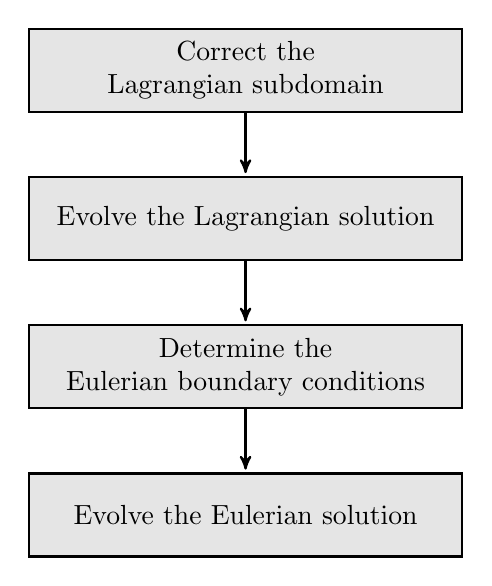
\begin{tikzpicture}
			[node distance=.8cm, start chain=going below,]
			\node[punktchain, join] (correct) {Correct the \\Lagrangian subdomain};
		    \node[punktchain, join] (evolveL) {Evolve the Lagrangian solution};
		    \node[punktchain, join] (bcE)     {Determine the \\Eulerian boundary conditions};
		    \node[punktchain, join] (evolveE) {Evolve the Eulerian solution};
		\end{tikzpicture}
		\caption{Flowchart of the simple coupling strategy. The flowchart shows the procedure to evolve both methods from $t_n$ to $t_{n+1}$.}
		\label{fig:flowchart_simpleCoupling}
	\end{figure}




% Summarize daenincks approach:
	% Methodology, algorithm
	% Domain decomposition
% Summarize stock's approach:
	% Methodology, algorithms
	% Resulted domain decomposition.


%%%%%%%%%%%%%%%%%%%%%%%%%%%%%%%%%%%%%%%%%%%%%%%%%%%%%%%%%%%%%%%%%%%%%%%%%%%%%%%%%%%%%%%%%%%%%%%%%%%%%%%%%%%%%%%%%%%%%%%%%%%%%%%%%%



%
    	
%    \appendix  
%    \addcontentsline{toc}{chapter}{Appendix}
%   	
\chapter{\texttt{pHyFlow} Code Structure}
\label{app:code}%

%\title{pHyFlow Code Structure}
%\author{Artur Palha, Lento Manickathan}

%\begin{document}
%\maketitle
%\begin{abstract}
The document outlines the \texttt{pHyFlow} code structure. The \texttt{pHyFlow} functions are organized into several classes. The functions related to the vortex particles are placed inside the \texttt{Blobs} class. The functions related to the panel problem are inside \texttt{Panels} class. The \texttt{LagrangianSolver} class is made to couple the functions of the vortex blobs and the vortex panel together. The functions of the Eulerian domain are placed inside the \texttt{EulerianSolver} class, where the Navier-stokes grid problem is solved. Finally, coupling of all the problems are done with the \texttt{HybridSolver} class. Note, all the classes are capable of handling multi-body / multi-domain problem within them and \texttt{LagrangianSolver} class and the \texttt{HybridSolver} class only couples methods together.\\

\underline{\texttt{pHyFlow} Structure:}
\begin{figure}[h]
\centering
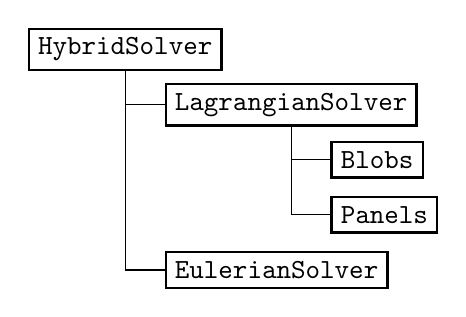
\begin{tikzpicture}[%
  grow via three points={one child at (0.5,-0.7) and
  two children at (0.5,-0.7) and (0.5,-1.4)},
  edge from parent path={(\tikzparentnode.south) |- (\tikzchildnode.west)}]
  \node {\texttt{HybridSolver}}
    child { node {\texttt{LagrangianSolver}}
    	child {node {\texttt{Blobs}}}
    	child {node {\texttt{Panels}}}  	
    }
    child [missing] {}				
    child [missing] {}				
    child { node {\texttt{EulerianSolver}}};
    %child { node [selected] {tex}
    %  child { node {generic}}
    %  child { node [optional] {latex}}
    %  child { node {plain}}
    %}
    %child [missing] {}
    %child { node {texdoc}};
\end{tikzpicture}
\end{figure}
%\end{abstract}
\newpage

\section*{\texttt{Blobs} Class}
The main structure of the \texttt{Blobs} class. This class contains all the function related to the calculation of the vortex blobs.
\begin{figure}[h]
\centering
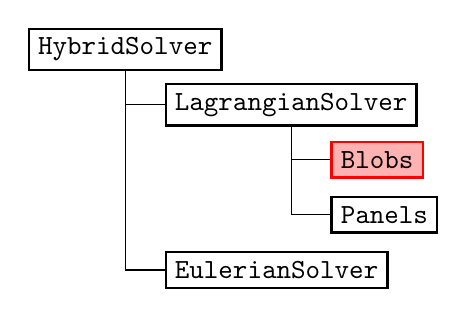
\begin{tikzpicture}[%
  grow via three points={one child at (0.5,-0.7) and
  two children at (0.5,-0.7) and (0.5,-1.4)},
  edge from parent path={(\tikzparentnode.south) |- (\tikzchildnode.west)}]
  \node {\texttt{HybridSolver}}
    child { node {\texttt{LagrangianSolver}}
    	child {node [selected] {\texttt{Blobs}}}
    	child {node {\texttt{Panels}}}  	
    }
    child [missing] {}				
    child [missing] {}				
    child { node {\texttt{EulerianSolver}}};
    %child { node [selected] {tex}
    %  child { node {generic}}
    %  child { node [optional] {latex}}
    %  child { node {plain}}
    %}
    %child [missing] {}
    %child { node {texdoc}};
\end{tikzpicture}
\end{figure}

\subsection*{Class structure:}
\begin{figure}[h]
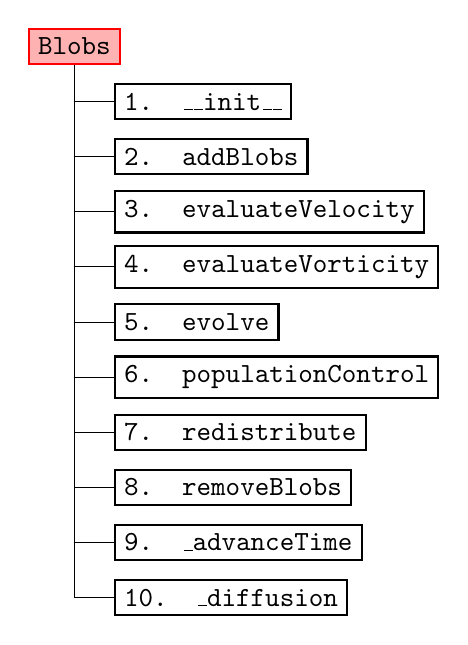
\begin{tikzpicture}[%
  grow via three points={one child at (0.5,-0.7) and
  two children at (0.5,-0.7) and (0.5,-1.4)},
  edge from parent path={(\tikzparentnode.south) |- (\tikzchildnode.west)}]
  \node [selected] {\texttt{Blobs}}
    child { node {\texttt{1. \_\_init\_\_}}}
    child { node {\texttt{2. addBlobs}}}
    child { node {\texttt{3. evaluateVelocity}}}                    
    child { node {\texttt{4. evaluateVorticity}}}   
    child { node {\texttt{5. evolve}}}    
    child { node {\texttt{6. populationControl}}}   
    child { node {\texttt{7. redistribute}}}    
	child { node {\texttt{8. removeBlobs}}}  
	child { node {\texttt{9. \_advanceTime}}}  	
	child { node {\texttt{10. \_diffusion}}};	
\end{tikzpicture}
\end{figure}

\subsection*{Attributes:}
\begingroup
\footnotesize
\begin{longtable}{|l|p{9cm}|}
	\hline
	\textbf{Attributes} & \textbf{Description}\\
	\toprule
    \texttt{blobControlParams} 		& The diffusion parameters. It is a dictionary containing all the parameters of the diffusion method used for the simulation. Contains: \texttt{stepRedistribution}, \texttt{stepPopulationControl}, \texttt{gThresholdLocal}, \texttt{gThresholdGlobal}.\\\hline
    \texttt{computationMethod} 		&\texttt{computationMethod} (tuple) with the type of Biot-Savart solver (\texttt{direct}, \texttt{fmm}) and the type of hardware to use (\texttt{cpu}, \texttt{gpu}).\\\hline
    \texttt{deltaTc} & The size of the convective time step $\Delta t_c$\\\hline
    \texttt{deltaTd} & The size of the convective time step $\Delta t_d$\\\hline
    \texttt{diffusionParams} & A dictionary containing all the parameters related to the computation of the diffusion step. Specifies the diffusion scheme and other specific parameters. Contains: \texttt{method}, \texttt{c2}.\\\hline
    \texttt{g} & The strength of the vortex blobs $\alpha$.\\          \hline
    \texttt{gThresholdGlobal} & Maximum value of variation of total vorticity due to the removal of blobs during population control.\\\hline
    \texttt{gThresholdLocal} & Minimum value of circulation to consider for each vortex blob when selecting blobs to remove during population control.\\    \hline      
    \texttt{h} & The size of the cell associated to the vortex blobs. Corresponds to the minimum spacing between the core of two neighboring cells. It is related to the core size of the blob, $\sigma$, and to the spacing $h$ by the expression $Ov = h/\sigma$.\\\hline          
    \texttt{integrationMethod} & \texttt{integrationMethod} (\texttt{fe}, \texttt{rk4}) the type of time integrator used: \texttt{fe} forward Euler, \texttt{rk4} Runge-Kutta $4^{th}$ order.\\ \hline
    \texttt{nu} & The fluid kinematic viscosity, used to calculate the diffusion coefficient: \texttt{c2} and diffusion time step \texttt{deltaTd}, $\Delta t_{d}$.\\          \hline
	\texttt{numBlobs} & The number of blobs.\\          \hline
	\texttt{overlap} & The overlap ratio between neighboring blobs.\\          \hline
	\texttt{plotVelocity} & A flag that defines if velocity is to be plotted or not.\\          \hline
	\texttt{sigma} & The core size of the vortex blobs.\\          \hline
	\texttt{stepDiffusion} & The frequency of diffusion steps.\\          \hline
	\texttt{stepPopulationControl} & The frequency of population control.\\          \hline
	\texttt{stepRedistribution} & The frequency of redistribution of blobs.\\          \hline
	\texttt{timeIntegrationParams} & A dictionary containing all time integration parameters of the simulation. Contains the definition of the time integration scheme possibly additional parameters specific to the scheme.\\ \hline
	\texttt{t} & The current time of the simulation.\\          \hline
	\texttt{tStep} & The current time step of the simulation.\\          \hline
	\texttt{velocityComputationParams} & A dictionary containing all the parameters related to the computation of induced velocities. Specifies computation scheme (direct or fmm) and hardware to use (cpu or gpu).\\          \hline
	\texttt{vInf} & The free stream velocity.\\          \hline
	\texttt{x} & The $x$ coordinates of the vortex blobs.\\          \hline
	\texttt{y} & The $y$ coordinates of the vortex blobs.\\          \hline	                                
    
                       
    \caption{Attributes of \texttt{Blobs} class and their description.}
    \label{tab:attributeBlobs}
\end{longtable}
\endgroup

\subsection*{\texttt{\_\_init\_\_}}
	\paragraph{Description:} Initialize the \texttt{Blobs} class with either the given input parameters or by a reading a \texttt{file} containing all the necessary parameters.\\
	
	\begin{tabular}{l|lp{7cm}}
		\multicolumn{2}{l}{\textbf{Input Parameters}} & \\ \hline
		\textit{File Name} & \multicolumn{2}{l}{Containing all the parameters to re-initalize the class.} \\ \cline{2-3}
		\multicolumn{3}{c}{--- or ---} \\ \cline{2-3}
		\multirow{4}{*}{\textit{Parameters}} & Vorticity Field &: \{\texttt{xBlob, yBlob, gBlob}\} or \{\texttt{wFunction, xBounds, yBounds}\}\\ \cline{2-3}
		& Blob parameters &: \texttt{overlap, h} \\ \cline{2-3}
		& Time Step parameters &: \texttt{deltaTc, nu, stepRedistribution, integrationMethod, computationMethod}\\ \cline{2-3}
		& Population control parameters &: \texttt{stepPopulationControl, gThreshold}\\ \cline{2-3}
	\end{tabular}\\
	
	\subsubsection*{Descriptions of the parameters:}
	\begin{tabular}{p{3.5cm}p{9cm}p{1cm}}
				\textit{Vorticity field} & & \textit{Default}\\ \hline
				\texttt{xBlob,yBlob} &:  the $x,y$ blob coordinates. & - \\
				\texttt{gBlob} &: the circulation $\Gamma_i$ associated to each of the vortex blobs. & - \\
				& & \\
				\multicolumn{2}{c}{\textit{--- or ---}} & \\
				& & \\
				\texttt{wExactFunction} &: the function that returns the exact value of vorticity $\omega$ at any given $x,y$ coordinates. &\\
				& 	\begin{tabular}{lp{10cm}}
						\textbf{Input parameters} &: \texttt{xEval,yEval}\\ 
						\textbf{Assigns} &: \texttt{-}\\ 			
						\textbf{Returns} &: \texttt{wEval}\\ 					
					\end{tabular} & - \\
				\texttt{xBounds, yBounds} &: the $x,y$ bounds of the domain where the particles was originally distributed. & - \\		 
	\end{tabular}\\
	\\ \\
	%	\begin{tabular}{lp{10cm}}
	%		\textbf{Input parameters} &: \texttt{xEval,yEval}\\ 
	%		\textbf{Assigns} &: \texttt{-}\\ 			
	%		\textbf{Returns} &: \texttt{vortEval}\\ 					
	%	\end{tabular}\\
	\begin{tabular}{p{3.5cm}p{9cm}p{1cm}}
				\multicolumn{2}{l}{\textit{Blob parameters}} & \textit{Default} \\ \hline				
				\texttt{overlap} &: the overlap ratio $h/\sigma$. & 1.0\\
				\texttt{h} &: the size of the cell $h$ associated to the blobs. \textit{Note:} Cells are square. & -\\
	\end{tabular}\\
	\\ \\
	\begin{tabular}{p{3.5cm}p{9cm}p{1cm}}
				\multicolumn{2}{l}{\textit{Time step parameters}} & \textit{Default}\\ \hline
				\texttt{deltaTc} &:  the size of the convective time step $\Delta t_c$. & - \\
				\texttt{nu} &: the fluid kinematic viscosity $\nu$, used to calculate the diffusion coefficient $c^2$ and diffusion time step size $\Delta T_d$.& - \\
				\texttt{stepRedistribution} &: the redistribution step frequency. & 1 \\
				\texttt{integrationMethod} &: the time integration method (\texttt{FE}: Forward euler , \texttt{RK4}: $4^{th}$ order Runge-Kutta). & RK4 \\
				\texttt{computationMethod} &: the calculation method to evolve the blobs, (\texttt{Direct}: Direct Method, \texttt{FMM}: Fast-Multipole Method) using (\texttt{CPU}, \texttt{GPU}). & \{FMM, GPU\}.\\
	\end{tabular}\\ 
    \\ \\ 
	\begin{tabular}{p{3.5cm}p{9cm}p{1cm}}
				\multicolumn{2}{l}{\textit{Population control parameters}} & \textit{Default} \\ \hline
				\texttt{stepPopulationControl} &: population control step frequency & 1.\\
				\texttt{gThreshold} &: the tuple with minimum \textbf{and} maximum value of the circulation $\Gamma_{min}$. & - \\
	\end{tabular}\\ 
    \\ \\  
	\begin{tabular}{p{3.5cm}p{9cm}p{1cm}}
				\multicolumn{2}{l}{\textit{Free stream velocity}} & \textit{Default}\\ \hline
				\texttt{vInf} &: The free-stream velocity function, returning the velocity action on the vortex blobs. & -\\		
				&		\begin{tabular}{lp{2cm}}
							\textbf{Input parameters} &: \texttt{t}\\ 
							\textbf{Assigns} &: \texttt{-}\\ 			
							\textbf{Returns} &: \texttt{vx,vy}\\ 					
						\end{tabular} & - \\
				
	\end{tabular}\\

\newpage
%%%%%%%%%%%%%%%%%%%%%%%%%%%%%%%%%%%%%%%%%%%%%%%%%%%%%%%%%%%%%%%%%%%%%%%%%%%%%%%%%%%%%%%%%%%%%%%%%%%%%%%%%%%%%%%%%%%%%%%%%%%%%%%%%%
%%%%%%%%%%%%%%%%%%%%%%%%%%%%%%%%%%%%%%%%%%%%%%%%%%%%%%%%%%%%%%%%%%%%%%%%%%%%%%%%%%%%%%%%%%%%%%%%%%%%%%%%%%%%%%%%%%%%%%%%%%%%%%%%%%

\section*{\texttt{Panels} class}
The main structure of the panel method class \texttt{Panels}. This class contains all the functions related to the calculation of panels.

\begin{figure}[h]
\centering
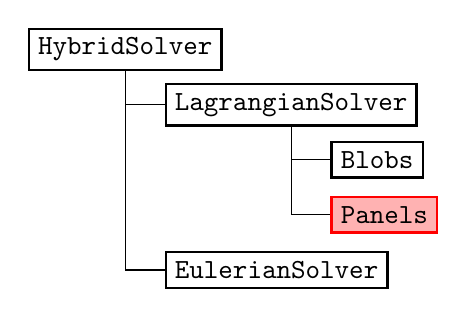
\begin{tikzpicture}[%
  grow via three points={one child at (0.5,-0.7) and
  two children at (0.5,-0.7) and (0.5,-1.4)},
  edge from parent path={(\tikzparentnode.south) |- (\tikzchildnode.west)}]
  \node {\texttt{HybridSolver}}
    child { node {\texttt{LagrangianSolver}}
    	child {node {\texttt{Blobs}}}
    	child {node [selected] {\texttt{Panels}}}  	
    }
    child [missing] {}				
    child [missing] {}				
    child { node {\texttt{EulerianSolver}}};
    %child { node [selected] {tex}
    %  child { node {generic}}
    %  child { node [optional] {latex}}
    %  child { node {plain}}
    %}
    %child [missing] {}
    %child { node {texdoc}};
\end{tikzpicture}
\end{figure}


\subsection*{Class structure:}
\begin{figure}[h]
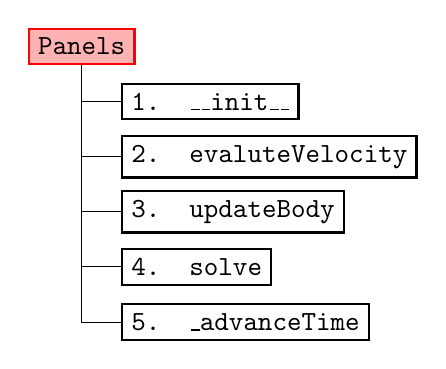
\begin{tikzpicture}[%
  grow via three points={one child at (0.5,-0.7) and
  two children at (0.5,-0.7) and (0.5,-1.4)},
  edge from parent path={(\tikzparentnode.south) |- (\tikzchildnode.west)}]
  \node [selected] {\texttt{Panels}}
    child { node {\texttt{1. \_\_init\_\_}}}
    child { node {\texttt{2. evaluteVelocity}}}                    
    child { node {\texttt{3. updateBody}}}                    
    child { node {\texttt{4. solve}}}                                        
    child { node {\texttt{5. \_advanceTime}}};
\end{tikzpicture}
\end{figure}


\subsection*{Attributes:}
\begingroup
\footnotesize
\begin{longtable}{|l|p{11cm}|}
	\hline
	\textbf{Attributes} & \textbf{Description}\\
	\toprule
    \texttt{A} 		& The inter-induction matrix $\mathbf{A}$, the LHS of the problem. \\ \hline
    \texttt{cmGlobal} & The global position vector for each of the $\mathbf{N}$
                       body, refining the position of the local panel $(0,0)$ in the
                       global coordinate system. \\\hline
    \texttt{deltaT} & The simulation time step size $\Delta T$\\ \hline
    \texttt{geometryKeys} & The dictionary containing all the parameters of the geometry. Contains: \texttt{xPanel} (the $x$ coordinate of the $\mathbf{M}$ panel corners.), \texttt{yPanel} (The $y$ coordinate of the $\mathbf{M}$ panel corners), \texttt{cmGlobal}, \texttt{thetaLocal}, \texttt{dPanel} (The off-set of the panel collocation point from the panel mid-point).  \\ \hline
    \texttt{nBodies} & The number of panel bodies.\\\hline
    \texttt{norm} & The $x$, $y$ normal vector of each panel.\\\hline
    \texttt{normCat} & The global concatenated $x$, $y$ component of the panel normal vector at each collocation points.\\          \hline
    \texttt{nPanels} & The number of panels in each body/geometry. \\ \hline
    \texttt{nPanelsTotal} & The total number of panels.\\    \hline      
    \texttt{panelKernel} & A string defining panel kernel type. \\\hline          
    \texttt{problemType} & A string defining the panel problem is of a \texttt{moving} type or of a \texttt{fixed} type.\\ \hline
    \texttt{solverCompParams} & The dictionary containing solver computation parameters.\\          \hline
	\texttt{sPanel} & The vortex sheet strengths $\gamma$ of $\mathbf{M}$ panels. \\          \hline
	\texttt{t} & The current time $t$ of the simulation.\\          \hline
	\texttt{tang} & The $x$, $y$ tangent vector of each panel.\\          \hline
	\texttt{tangCat} & The global concatenated $x$, $y$ component of the panel
	                  normal vector at each collocation points.\\          \hline
	\texttt{thetaLocal} & The local rotation angle $\theta$ w.r.t to the local
	                     coordinate system. The rotational will be performed around
	                     the local reference point $(0,0)$, i.e around the global center of rotation point \texttt{cmGlobal}.\\          \hline
	\texttt{tStep} & The current step of the simulation.\\          \hline
	\texttt{velCompParams} & A dictionary containing the velocity computation parameters, method and hardware.\\          \hline
	\texttt{xyCPGlobal} & The global $x$, $y$ coordinate of the panel collocation
	                     points.\\ \hline
	\texttt{xyCPGlobalCat} & The global concatenated $x$, $y$ coordinate of the
	                        panel collocation points.\\          \hline
	\texttt{xyPanelGlobal} & The global $x$, $y$ coordinate of the panel bodies.\\          \hline
	\texttt{xyPanelGlobalCat} & The global concatenated $x$, $y$ coordinate of the
	                           panel bodies.\\          \hline
	\texttt{xyPanelLocal} & The local $x$, $y$ coordinate of the panel bodies.\\          \hline
                       
    \caption{Attributes of \texttt{Panels} class and their description.}
    \label{tab:attributesPanels}
\end{longtable}
\endgroup


\subsection*{\texttt{\_\_init\_\_}}
	\begin{tabular}{l|lp{7cm}}
		\multicolumn{2}{l}{\textbf{Input Parameters}} & \\ \hline
		\textit{File Name} & \multicolumn{2}{l}{Containing all the parameters to re-initalize the class.} \\ \hline
		\multirow{2}{*}{\textit{Parameters}} & Panel coordinates &: \{\texttt{xCP, yCP, xPanel, yPanel, cmGlobal, thetaLocal}\}\\ \cline{2-3}
		& External velocity &: \texttt{externVel} \\ \cline{2-3}
	\end{tabular}
	\paragraph{Description:} Initialize the \texttt{panels} class with the given input parameters. In the case of a multibody problem, a list of panel coordinates can be given and internally it takes care of the inter-coupling.\\
	\\
	\begin{tabular}{lp{10cm}}
				\textit{Panel coordinates} & \\ \hline
				\texttt{xCP,yCP} &:  the local $x,y$-coordinates of the panel collocation points.\\ 
				\texttt{xPanel,yPanel} &: the local coordinate of the panel edges. \textit{Note}: Should have a closed loop (end with initial point coordinates).\\ 
				\texttt{cmGlobal} &:  the position of reference points of a given panel body.\\
				\texttt{thetaLocal} &:  the rotational angles of the panel body axes w.r.t to the global $x$-axis.\\
	\end{tabular}\\ 
    \\ \\
	\begin{tabular}{lp{10cm}}
				\textit{External velocity} & \\ \hline
				\texttt{externVel} &:  Reference to an external velocity \textbf{function} acting of the panels. For the panel case, the external velocity will the induced velocity of the blobs + freestream \texttt{vortexBlob.evaluateVelocity}.\\
	\end{tabular}\\
	
		\begin{tabular}{lp{10cm}}
			\textbf{Input parameters} &: \texttt{xCP,yCP}\\ 
			\textbf{Assigns} &: \texttt{-}\\ 			
			\textbf{Returns} &: \texttt{vxCP,vyCP}\\ 					
		\end{tabular}\\


\newpage
%%%%%%%%%%%%%%%%%%%%%%%%%%%%%%%%%%%%%%%%%%%%%%%%%%%%%%%%%%%%%%%%%%%%%%%%%%%%%%%%%%%%%%%%%%%%%%%%%%%%%%%%%%%%%%%%%%%%%%%%%%%%%%%%%%
%%%%%%%%%%%%%%%%%%%%%%%%%%%%%%%%%%%%%%%%%%%%%%%%%%%%%%%%%%%%%%%%%%%%%%%%%%%%%%%%%%%%%%%%%%%%%%%%%%%%%%%%%%%%%%%%%%%%%%%%%%%%%%%%%%

\section*{\texttt{LagrangianSolver} Class}
The main structure of the \texttt{Blobs} + \texttt{Panels} (LagrangianSolver) class. This class contains all the function related to the calculations of panel with vortex blobs.

\begin{figure}[h]
\centering
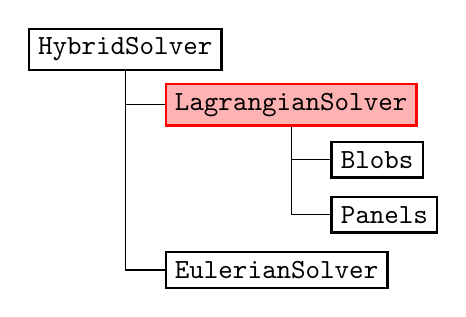
\begin{tikzpicture}[%
  grow via three points={one child at (0.5,-0.7) and
  two children at (0.5,-0.7) and (0.5,-1.4)},
  edge from parent path={(\tikzparentnode.south) |- (\tikzchildnode.west)}]
  \node {\texttt{HybridSolver}}
    child { node [selected] {\texttt{LagrangianSolver}}
    	child {node {\texttt{Blobs}}}
    	child {node {\texttt{Panels}}}  	
    }
    child [missing] {}				
    child [missing] {}				
    child { node {\texttt{EulerianSolver}}};
    %child { node [selected] {tex}
    %  child { node {generic}}
    %  child { node [optional] {latex}}
    %  child { node {plain}}
    %}
    %child [missing] {}
    %child { node {texdoc}};
\end{tikzpicture}
\end{figure}

\subsection*{Class structure:}
\begin{figure}[h]
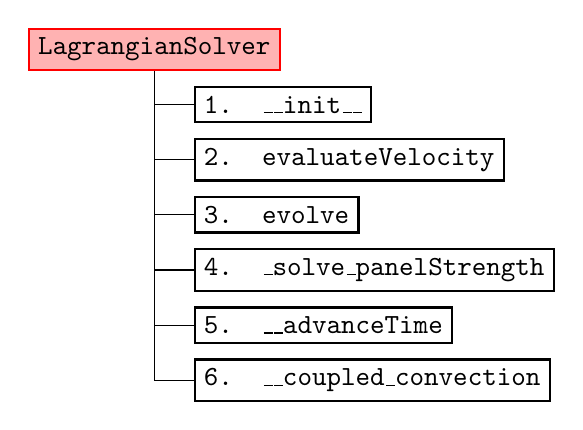
\begin{tikzpicture}[%
  grow via three points={one child at (0.5,-0.7) and
  two children at (0.5,-0.7) and (0.5,-1.4)},
  edge from parent path={(\tikzparentnode.south) |- (\tikzchildnode.west)}]
  \node [selected] {\texttt{LagrangianSolver}}
    child { node {\texttt{1. \_\_init\_\_}}}
    child { node {\texttt{2. evaluateVelocity}}}
    child { node {\texttt{3. evolve}}}
    child { node {\texttt{4. \_solve\_panelStrength}}}                        
    child { node {\texttt{5. \_\_advanceTime}}}                        
    child { node {\texttt{6. \_\_coupled\_convection}}};                       

\end{tikzpicture}
\end{figure}

\subsection*{Attributes:}
\begingroup
\footnotesize
\begin{longtable}{|l|p{12cm}|}
	\hline
	\textbf{Attributes} & \textbf{Description}\\
	\toprule
    \texttt{deltaT}     & The inter-induction matrix $\mathbf{A}$, the LHS of the problem. \\ \hline
    \texttt{gTotal}     & The total circulation of the Lagrangian domain. \\ \hline    
	\texttt{t} & The current time $t$ of the simulation.\\          \hline
	\texttt{tStep} & The current step of the simulation.\\          \hline
	\texttt{vInf} & The $x$, $y$ component of the free-stream velocity.\\          \hline	
	\texttt{Blobs} & The vortex blobs class \texttt{Blobs}.\\          \hline	
	\texttt{Panels} & The vortex panels class \texttt{Panels}.\\          \hline			
                      
    \caption{Attributes of \texttt{LagrangianSolver} class and their description.}
    \label{tab:attributesLagrangianSolver}
\end{longtable}
\endgroup


\subsection*{\texttt{\_\_init\_\_}}
	\begin{tabular}{l|lp{7cm}}
		\multicolumn{2}{l}{\textbf{Input Parameters}} & \\ \hline
		\textit{File Name} & \multicolumn{2}{l}{Containing all the parameters to re-initalize the class.} \\ \hline
		\multirow{2}{*}{\textit{Parameters}} & \texttt{vortexBlobs} &: \{\texttt{vortexBlobs}\} class. \\ \cline{2-3}
		& \texttt{panels} &: \texttt{panels} class. \\ \cline{2-3}
	\end{tabular}
	\paragraph{Description:} Initialize the \texttt{vortexMethod} class using \textbf{vortexBlob}+\textbf{panelMethod} \\ classes.
	\paragraph{Input parameters:}
	\begin{list}{\quad}{}
	\item \texttt{Blobs}: vortex particle class
	\item \texttt{Panels}: panel method class				
	\end{list}


\newpage
%%%%%%%%%%%%%%%%%%%%%%%%%%%%%%%%%%%%%%%%%%%%%%%%%%%%%%%%%%%%%%%%%%%%%%%%%%%%%%%%%%%%%%%%%%%%%%%%%%%%%%%%%%%%%%%%%%%%%%%%%%%%%%%%%%
%%%%%%%%%%%%%%%%%%%%%%%%%%%%%%%%%%%%%%%%%%%%%%%%%%%%%%%%%%%%%%%%%%%%%%%%%%%%%%%%%%%%%%%%%%%%%%%%%%%%%%%%%%%%%%%%%%%%%%%%%%%%%%%%%%

\section*{\texttt{EulerianSolver}}
The main structure for the Navier-stokes class \texttt{EulerianSolver}. This class contains all the functions related to computation of the Navier-stokes problem. Below is set of functions that acts as the interface to the class.

\begin{figure}[h]
\centering
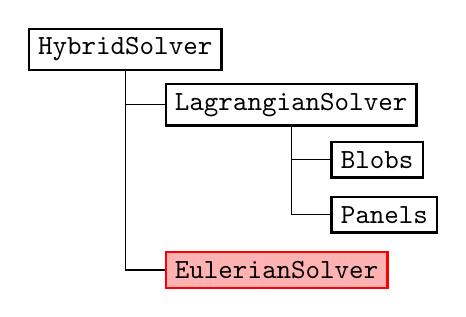
\begin{tikzpicture}[%
  grow via three points={one child at (0.5,-0.7) and
  two children at (0.5,-0.7) and (0.5,-1.4)},
  edge from parent path={(\tikzparentnode.south) |- (\tikzchildnode.west)}]
  \node {\texttt{HybridSolver}}
    child { node {\texttt{LagrangianSolver}}
    	child {node {\texttt{Blobs}}}
    	child {node {\texttt{Panels}}}  	
    }
    child [missing] {}				
    child [missing] {}				
    child { node [selected] {\texttt{EulerianSolver}}};
    %child { node [selected] {tex}
    %  child { node {generic}}
    %  child { node [optional] {latex}}
    %  child { node {plain}}
    %}
    %child [missing] {}
    %child { node {texdoc}};
\end{tikzpicture}
\end{figure}



\subsection*{Class structure:}
\begin{figure}[h]
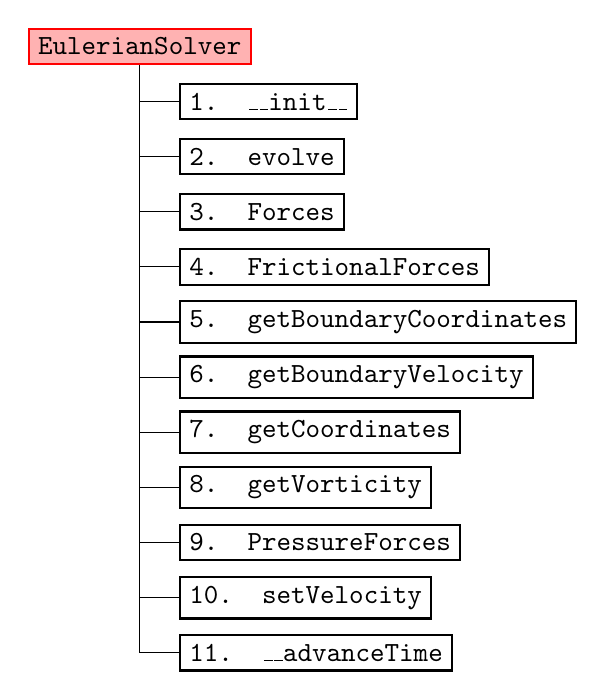
\begin{tikzpicture}[%
  grow via three points={one child at (0.5,-0.7) and
  two children at (0.5,-0.7) and (0.5,-1.4)},
  edge from parent path={(\tikzparentnode.south) |- (\tikzchildnode.west)}]
  \node [selected] {\texttt{EulerianSolver}}
    child { node {\texttt{1. \_\_init\_\_}}}
    child { node {\texttt{2. evolve}}}
    child { node {\texttt{3. Forces}}}
    child { node {\texttt{4. FrictionalForces}}}
    child { node {\texttt{5. getBoundaryCoordinates}}}                            
    child { node {\texttt{6. getBoundaryVelocity}}}                    
    child {node  {\texttt{7. getCoordinates}}}            
    child { node {\texttt{8. getVorticity}}}                                   
    child { node {\texttt{9. PressureForces}}}
    child { node {\texttt{10. setVelocity}}}
    child { node {\texttt{11. \_\_advanceTime}}};
\end{tikzpicture}
\end{figure}


\subsection*{Attributes:}
\begingroup
\footnotesize
\begin{longtable}{|l|p{11cm}|}
	\hline
	\textbf{Attributes} & \textbf{Description}\\
	\toprule
    \texttt{deltaT} 		& The time step size $\Delta t$. \\ \hline
    \texttt{deltaTMax} 		& The maximum allowable time step size $\max\{\Delta t\}$.\\ \hline
    \texttt{cfl} 			& The Courant–Friedrichs–Lewy condition stability number CFL. \\ \hline        
    \texttt{cmGlobal} 		& The $x$, $y$ position of the mesh local reference point $(0,0)$ in the global coordinates. \\ \hline        
    \texttt{hMin} 			& The minimum mesh cell size. \\ \hline        
    \texttt{nu} 			& The fluid kinematic viscosity $\nu$.  \\ \hline        
    \texttt{probeGridMesh} 	& The \textit{local} $x$, $y$ coordinates of the probe grid mesh. \\ \hline            
    \texttt{probeGridParams}& The dictionary containing all the parameters of the probe grid for extracting the vorticity data. \\ \hline            
    \texttt{solverParams} 	& The dictionary file containing all the solver parameters.  \\ \hline                
    \texttt{t} 				& The current time of the simulation. \\ \hline                    
    \texttt{thetaLocal} 	& The local rotational angle $\theta$ of the mesh domain. Therefore, the rotation will be done about local reference  point $(0,0)$, i.e \texttt{cmGlobal} in the global coordinate system.\\ \hline                            
    \texttt{tStep} 			& The current step of the simulation. \\ \hline                    
    \texttt{uMax} 			& The maximum fluid velocity $\max\{\mathbf{u}\}$. \\ \hline
    
    \caption{Attributes of \texttt{EulerianSolver} class and their description.}
    \label{tab:attributeEulerian}
\end{longtable}
\endgroup


\subsection*{\texttt{\_\_init\_\_}}
	\paragraph{Description:} Initialize the \texttt{navierStokes} class either using a \texttt{fileName} containing all the necessary parameter for initialization or by explicitly inputing the parameters.\\

	\begin{tabular}{l|lp{7cm}}
		\multicolumn{2}{l}{\textbf{Input Parameters}} & \\ \hline
		\textit{File Name} & \multicolumn{2}{l}{Containing all the parameters to re-initalize the class.} \\ \hline
		\multicolumn{3}{c}{-- or --} \\ \hline
		\multirow{5}{*}{\textit{Parameters}} & Mesh data &: \texttt{mesh, boundaryDomains}\\ \cline{2-3}
		& Geometry position &: \texttt{cmGlobal, thetaLocal} \\ \cline{2-3}
		& Fluid parameters &: \texttt{uMax, nu}\\ \cline{2-3}
		& Solver options &: \texttt{cfl}\\ \cline{2-3}
		& Probe grid parameters &: \texttt{x0, y0, Lx, Ly, hx, hy}\\ \cline{2-3}

	\end{tabular}\\
	\subsubsection*{Description of the parameters:}
	
	\begin{tabular}{lp{10cm}}
				\textit{Mesh data} & \\ \hline
				\texttt{mesh} &: the mesh data file.\\ 
				\texttt{boundaryDomains} &: the boundary mesh domain data file.\\ 			
	\end{tabular}\\ 
    \\ \\
	\begin{tabular}{lp{10cm}}
				\textit{Geometry position} & \\ \hline
				\texttt{cmGlobal} &: the $x,y$ position of the geometry in global coordinates.\\ 
				\texttt{thetaGlobal} &: the rotation angle (in $rad$) of the geometry in global coordinate system.\\ 			
	\end{tabular}\\
    \\ \\
	\begin{tabular}{lp{10cm}}
				\textit{Fluid parameters} & \\ \hline
				\texttt{uMax} &: the maximum fluid velocity $U_{max}$. Used to determine the maximum time step size $\Delta t_{max}$.\\ 
				\texttt{nu} &: the fluid kinematic viscosity $\nu$, for incompressible navier-stokes problem.\\ 			
	\end{tabular}\\	
    \\ \\
	\begin{tabular}{lp{10cm}}
				\textit{Solver options} & \\ \hline
				\texttt{cfl} &: the $CFL$ stability parameter. If explicit time marching scheme, $CFL<1$.\\ 		
	\end{tabular}\\	
    \\ \\
	\begin{tabular}{lp{10cm}}
				\textit{Probe grid parameters} & \\ \hline
				\texttt{x0,y0} &: the $x,y$ coordinate of the origin of the probe grid.\\ 
				\texttt{Lx,Ly} &: the $x,y$ size (width and height) of the probing grid.\\ 			
				\texttt{hx,hy} &: the $x,y$ spacing of the probe grid cell.\\ 							
	\end{tabular}\\	


\newpage
%%%%%%%%%%%%%%%%%%%%%%%%%%%%%%%%%%%%%%%%%%%%%%%%%%%%%%%%%%%%%%%%%%%%%%%%%%%%%%%%%%%%%%%%%%%%%%%%%%%%%%%%%%%%%%%%%%%%%%%%%%%%%%%%%%
%%%%%%%%%%%%%%%%%%%%%%%%%%%%%%%%%%%%%%%%%%%%%%%%%%%%%%%%%%%%%%%%%%%%%%%%%%%%%%%%%%%%%%%%%%%%%%%%%%%%%%%%%%%%%%%%%%%%%%%%%%%%%%%%%%


\section*{\texttt{HybridSolver} Class}
The main structure for the hybrid class \texttt{HybridSolver}. This class contains all the functions related to computation of the hybrid problem.

\begin{figure}[h]
\centering
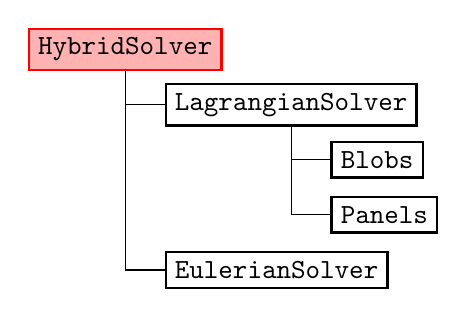
\begin{tikzpicture}[%
  grow via three points={one child at (0.5,-0.7) and
  two children at (0.5,-0.7) and (0.5,-1.4)},
  edge from parent path={(\tikzparentnode.south) |- (\tikzchildnode.west)}]
  \node [selected] {\texttt{HybridSolver}}
    child { node {\texttt{LagrangianSolver}}
    	child {node {\texttt{Blobs}}}
    	child {node {\texttt{Panels}}}  	
    }
    child [missing] {}				
    child [missing] {}				
    child { node {\texttt{EulerianSolver}}};
    %child { node [selected] {tex}
    %  child { node {generic}}
    %  child { node [optional] {latex}}
    %  child { node {plain}}
    %}
    %child [missing] {}
    %child { node {texdoc}};
\end{tikzpicture}
\end{figure}

\subsection*{Class structure:}
\begin{figure}[h]
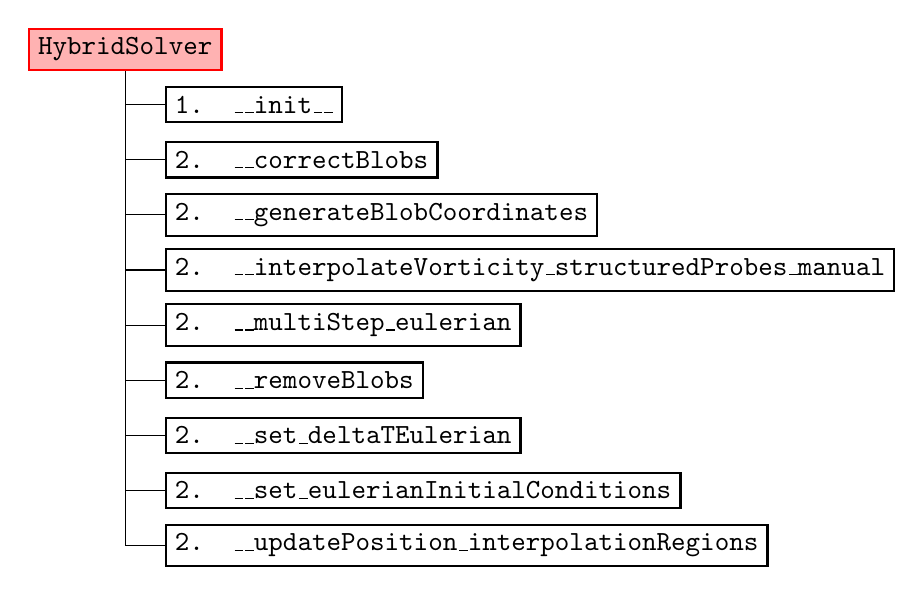
\begin{tikzpicture}[%
  grow via three points={one child at (0.5,-0.7) and
  two children at (0.5,-0.7) and (0.5,-1.4)},
  edge from parent path={(\tikzparentnode.south) |- (\tikzchildnode.west)}]
  \node [selected] {\texttt{HybridSolver}}
    child { node {\texttt{1. \_\_init\_\_}}}
    child { node {\texttt{2. \_\_correctBlobs}}}
    child { node {\texttt{2. \_\_generateBlobCoordinates}}}
    child { node {\texttt{2. \_\_interpolateVorticity\_structuredProbes\_manual}}}
    child { node {\texttt{2. \_\_multiStep\_eulerian}}}
    child { node {\texttt{2. \_\_removeBlobs}}}
    child { node {\texttt{2. \_\_set\_deltaTEulerian}}}    
    child { node {\texttt{2. \_\_set\_eulerianInitialConditions}}}        
    child { node {\texttt{2. \_\_updatePosition\_interpolationRegions}}};
\end{tikzpicture}
\end{figure}


\subsection*{Attributes:}
\begingroup
\footnotesize
\begin{longtable}{|l|p{10cm}|}
	\hline
	\textbf{Attributes} & \textbf{Description}\\
	\toprule
    \texttt{deltaTEulerian} 		& The time step size of the Eulerian sub-domain $\Delta t_E$. \\ \hline
    \texttt{deltaTLagrangian} 		& The time step size of the Lagrangian sub-domain $\Delta t_L$.\\ \hline
	\texttt{nu} 			& The fluid kinematic viscosity $\nu$.  \\ \hline        
    \texttt{t} 				& The current time $t$ of the simulation. \\ \hline                    
    \texttt{tStep} 			& The current step of the simulation. \\ \hline                    
    \texttt{vInf} 			& The $x$, $y$ component of the free-stream velocity. \\ \hline
    \texttt{interpolationRegion} & The dictionary containing the \texttt{surfacePolygon} and \texttt{boundaryPolygon} defining the boundaries of the interpolation region for each Eulerian sub-domains. The geometry is identified by the keys of the Eulerian sub-domain found in \texttt{multiEulerian}. The coordinates are defined in local coordinate system of the Eulerian grid and will be transformed (rotated + moved) during the evolution step. \\ \hline
    \texttt{lagrangian} 	& The Lagrangian solver class contains all the parameters related to simulation the flow in lagrangian sub-domain. \\ \hline
    \texttt{multiEulerian} 	& The \texttt{multiEulerian} is solver class containing all the Eulerian sub-domains of the hybrid problem. \\ \hline
    
    \caption{Attributes of \texttt{HybridSolver} class and their description.}
    \label{tab:attributeHybrid}
\end{longtable}
\endgroup


\subsection*{\texttt{\_\_init\_\_}}
	\begin{tabular}{l|lp{7cm}}
		\multicolumn{2}{l}{\textbf{Input Parameters}} & \\ \hline
		\textit{File Name} & \multicolumn{2}{l}{Containing all the parameters to re-initalize the class.} \\ \hline
		\multirow{4}{*}{\textit{Parameters}} & \texttt{vortexMethod} &: \{\texttt{vortexMethod}\} class.\\ \cline{2-3}
		& \texttt{navierStokes} &: \texttt{navierStokes} class. \\ \cline{2-3}
		& Interpolation region &: \texttt{xPolygon, yPolygon}\\ \cline{2-3}
		& Motion functions &: \texttt{T, cmGlobal, thetaGlobal, cmDotGlobal, thetaDotGlobal}\\ \cline{2-3}
	\end{tabular}\\
	
	\paragraph{Description:} Initialize the \texttt{hybrid} class using \texttt{LagrangianSolver} + \texttt{EulerianSolver} classes.
	\paragraph{Input parameters:}
	\begin{list}{\quad}{}
	\item \texttt{LagrangianSolver}: The vortex method containing \texttt{Blobs} and \textbf{Panels} classes which can already handle the multi-body problem.
	\item \texttt{EulerianSolver}: The Navier-Stokes grid solver class (if multiple: list of \\ \texttt{EulerianSolver} classes). The number of navier-stokes class has to be same as the number of vortex panels.
	\item \textbf{Interpolation Region}: the Navier-Stokes class (if multiple: list of \\ \texttt{EulerianSolver} classes). Should be equal to number of Navier-Stokes classes. The interpolation region should be defined as list of $x,y$ coordinates of the polygon of the interpolation region.
	\item \textbf{Motion function}: the function describing the motion of all the geometries in the hybrid class.
	\end{list}
	
	\begin{tabular}{lp{10cm}}
		\textit{Interpolation Regions} & \\ \hline
		\texttt{xPolygon,yPolygon}: & the new $x,y$ coordinate of the polygons description the interpolation region. The polygon should have a closed loop (end  with starting coordinates) before continuing to the next polygon. In the case of multiple polygons, a list of \texttt{xPolygon,yPolygon} should be given and should be as many as the number of navier-stokes domain.\\ 
	\end{tabular} \vspace{5 mm}

	\begin{tabular}{lp{10cm}}
		\textit{Motion function} & \\ \hline
		\texttt{T} &: the current time.\\ 
		\texttt{cmGlobal} &: a list of new positions of the geometries in the hybrid problem.\\ 
		\texttt{thetaGlobal} &: a list of new rotational angle of the geometries in the hybrid problem.\\ 		
		\texttt{cmDotGlobal} &: a list of current displacement velocity of the geometries in the hybrid problem.\\ 				
		\texttt{thetaDotGlobal} &: a list of current rotational velocity of the geometries in the hybrid problem.\\ 						
	\end{tabular} \vspace{5 mm}

	\begin{tabular}{lp{10cm}}
		\textbf{Input parameters} &: \texttt{T}\\ 
		\textbf{Assigns} &: \texttt{-}\\ 			
		\textbf{Returns} &: \texttt{cmGlobal,thetaGlobal,cmDotGlobal,thetaDotGlobal}\\ 					
	\end{tabular}



% Include all the documents
%\section{\texttt{vortexBlobs}}
The main structure of the \texttt{vortexBlobs} class. This class contains all the function related to the calculation of the vortex blobs.
\begin{figure}[h]
\centering
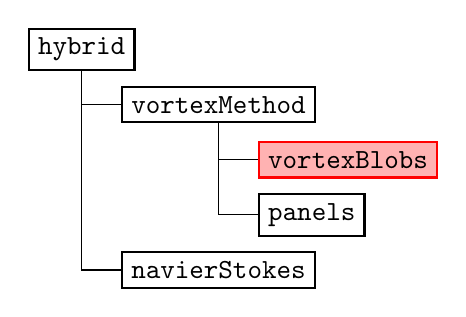
\begin{tikzpicture}[%
  grow via three points={one child at (0.5,-0.7) and
  two children at (0.5,-0.7) and (0.5,-1.4)},
  edge from parent path={(\tikzparentnode.south) |- (\tikzchildnode.west)}]
  \node {\texttt{hybrid}}
    child { node {\texttt{vortexMethod}}
    	child {node [selected] {\texttt{vortexBlobs}}}
    	child {node {\texttt{panels}}}  	
    }
    child [missing] {}				
    child [missing] {}				
    child { node {\texttt{navierStokes}}};
    %child { node [selected] {tex}
    %  child { node {generic}}
    %  child { node [optional] {latex}}
    %  child { node {plain}}
    %}
    %child [missing] {}
    %child { node {texdoc}};
\end{tikzpicture}
\end{figure}

\subsection*{Class structure:}
\begin{figure}[h]
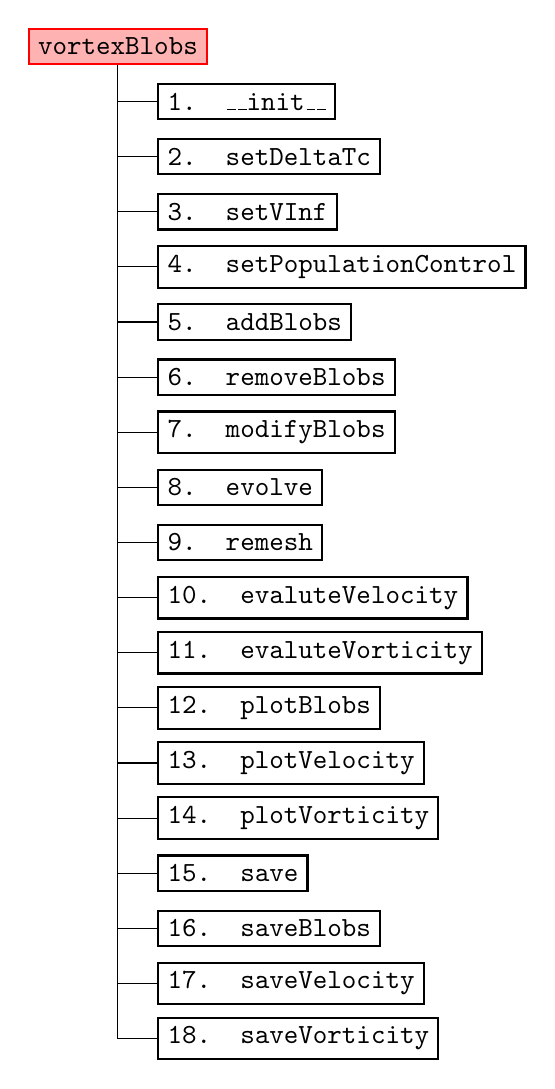
\begin{tikzpicture}[%
  grow via three points={one child at (0.5,-0.7) and
  two children at (0.5,-0.7) and (0.5,-1.4)},
  edge from parent path={(\tikzparentnode.south) |- (\tikzchildnode.west)}]
  \node [selected] {\texttt{vortexBlobs}}
    child { node {\texttt{1. \_\_init\_\_}}}
    child { node {\texttt{2. setDeltaTc}}}
    child { node {\texttt{3. setVInf}}}    
    child { node {\texttt{4. setPopulationControl}}}
    child { node {\texttt{5. addBlobs}}}
    child { node {\texttt{6. removeBlobs}}}    
    child { node {\texttt{7. modifyBlobs}}}    
    child { node {\texttt{8. evolve}}}    
    child { node {\texttt{9. remesh}}}    
    child { node {\texttt{10. evaluteVelocity}}}                    
    child { node {\texttt{11. evaluteVorticity}}}                        
    child { node {\texttt{12. plotBlobs}}}                        
    child { node {\texttt{13. plotVelocity}}}                        
    child { node {\texttt{14. plotVorticity}}}                            
    child { node {\texttt{15. save}}}                        
    child { node {\texttt{16. saveBlobs}}}                                        
    child { node {\texttt{17. saveVelocity}}}                                            
    child { node {\texttt{18. saveVorticity}}};
%    child { node [optional] {19. \texttt{\_generateBlobs}}}
%    child { node [optional] {20. \texttt{\_populationControl}}};        
        %child { node [selected] {tex}
    %  child { node {generic}}
    %  child { node [optional] {latex}}
    %  child { node {plain}}
    %}
    %child { node {texdoc}};
\end{tikzpicture}
\end{figure}

%\subsection*{Structure:}
%\begin{table}[h]
%\begin{tabular}{rl}
%	\texttt{vortexBlobs}: &  \\ \hline
%	-- & \texttt{\_\_init\_\_} \\
%	& \\
%	-- & \texttt{set\_deltaTc} \\ 
%	-- & \texttt{set\_popControlParameters} \\ 
%	-- & \texttt{addBlobs} \\ 
%	-- & \texttt{removeBlobs} \\ 
%	-- & \texttt{modifyBlobs} \\ 
%	-- & \texttt{evolve} \\ 
%	-- & \texttt{remesh} \\ 
%	-- & \texttt{evaluteVelocity} \\ 
%	-- & \texttt{evaluteVorticity} \\ 
%	-- & \texttt{plotBlobs} \\	
%	-- & \texttt{plotVelocity} \\
%	-- & \texttt{plotVorticity} \\
%	-- & \texttt{saveClass} \\ 
%	-- & \texttt{saveBlob} \\ 
%	-- & \texttt{saveVelocity} \\ 	
%	-- & \texttt{saveVorticity} \\ 
%	-- & \texttt{saveBlobPlot} \\ 
%	-- & \texttt{saveVelocityPlot} \\ 	
%	-- & \texttt{saveVorticityPlot} \\ 		
%	& \\
%	-- & \texttt{\_generateParticles} \\ 
%	-- & \texttt{\_popControl} \\
%\end{tabular}
%\end{table}

\newpage



\subsection{\texttt{\_\_init\_\_}}
	\paragraph{Description:} Initialize the \texttt{vortexBlobs} class with either the given input parameters or by a reading a \texttt{file} containing all the necessary parameters.\\
	
	\begin{tabular}{l|lp{7cm}}
		\multicolumn{2}{l}{\textbf{Input Parameters}} & \\ \hline
		\textit{File Name} & \multicolumn{2}{l}{Containing all the parameters to re-initalize the class.} \\ \cline{2-3}
		\multicolumn{3}{c}{--- or ---} \\ \cline{2-3}
		\multirow{4}{*}{\textit{Parameters}} & Vorticity Field &: \{\texttt{xBlob, yBlob, gBlob}\} or \{\texttt{wFunction, xBounds, yBounds}\}\\ \cline{2-3}
		& Blob parameters &: \texttt{overlap, h} \\ \cline{2-3}
		& Time Step parameters &: \texttt{deltaTc, nu, stepRedistribution, integrationMethod, computationMethod}\\ \cline{2-3}
		& Population control parameters &: \texttt{stepPopulationControl, gThreshold}\\ \cline{2-3}
	\end{tabular}\\
	
	\subsubsection*{Descriptions of the parameters:}
	\begin{tabular}{p{3.5cm}p{9cm}p{1cm}}
				\textit{Vorticity field} & & \textit{Default}\\ \hline
				\texttt{xBlob,yBlob} &:  the $x,y$ blob coordinates. & - \\
				\texttt{gBlob} &: the circulation $\Gamma_i$ associated to each of the vortex blobs. & - \\
				& & \\
				\multicolumn{2}{c}{\textit{--- or ---}} & \\
				& & \\
				\texttt{wExactFunction} &: the function that returns the exact value of vorticity $\omega$ at any given $x,y$ coordinates. &\\
				& 	\begin{tabular}{lp{10cm}}
						\textbf{Input parameters} &: \texttt{xEval,yEval}\\ 
						\textbf{Assigns} &: \texttt{-}\\ 			
						\textbf{Returns} &: \texttt{wEval}\\ 					
					\end{tabular} & - \\
				\texttt{xBounds, yBounds} &: the $x,y$ bounds of the domain where the particles was originally distributed. & - \\		 
	\end{tabular}\\
	\\ \\
	%	\begin{tabular}{lp{10cm}}
	%		\textbf{Input parameters} &: \texttt{xEval,yEval}\\ 
	%		\textbf{Assigns} &: \texttt{-}\\ 			
	%		\textbf{Returns} &: \texttt{vortEval}\\ 					
	%	\end{tabular}\\
	\begin{tabular}{p{3.5cm}p{9cm}p{1cm}}
				\multicolumn{2}{l}{\textit{Blob parameters}} & \textit{Default} \\ \hline				
				\texttt{overlap} &: the overlap ratio $h/\sigma$. & 1.0\\
				\texttt{h} &: the size of the cell $h$ associated to the blobs. \textit{Note:} Cells are square. & -\\
	\end{tabular}\\
	\\ \\
	\begin{tabular}{p{3.5cm}p{9cm}p{1cm}}
				\multicolumn{2}{l}{\textit{Time step parameters}} & \textit{Default}\\ \hline
				\texttt{deltaTc} &:  the size of the convective time step $\Delta t_c$. & - \\
				\texttt{nu} &: the fluid kinematic viscosity $\nu$, used to calculate the diffusion coefficient $c^2$ and diffusion time step size $\Delta T_d$.& - \\
				\texttt{stepRedistribution} &: the redistribution step frequency. & 1 \\
				\texttt{integrationMethod} &: the time integration method (\texttt{FE}: Forward euler , \texttt{RK4}: $4^{th}$ order Runge-Kutta). & RK4 \\
				\texttt{computationMethod} &: the calculation method to evolve the blobs, (\texttt{Direct}: Direct Method, \texttt{FMM}: Fast-Multipole Method) using (\texttt{CPU}, \texttt{GPU}). & \{FMM, GPU\}.\\
	\end{tabular}\\ 
    \\ \\ 
	\begin{tabular}{p{3.5cm}p{9cm}p{1cm}}
				\multicolumn{2}{l}{\textit{Population control parameters}} & \textit{Default} \\ \hline
				\texttt{stepPopulationControl} &: population control step frequency & 1.\\
				\texttt{gThreshold} &: the tuple with minimum \textbf{and} maximum value of the circulation $\Gamma_{min}$. & - \\
	\end{tabular}\\ 
    \\ \\  
	\begin{tabular}{p{3.5cm}p{9cm}p{1cm}}
				\multicolumn{2}{l}{\textit{Free stream velocity}} & \textit{Default}\\ \hline
				\texttt{vInf} &: The free-stream velocity function, returning the velocity action on the vortex blobs. & -\\		
				&		\begin{tabular}{lp{10cm}}
							\textbf{Input parameters} &: \texttt{t}\\ 
							\textbf{Assigns} &: \texttt{-}\\ 			
							\textbf{Returns} &: \texttt{vx,vy}\\ 					
						\end{tabular} & - \\
				
	\end{tabular}\\


\subsection{\texttt{setDeltaTc}}
	\paragraph{Description:} Function change the convective time step size $\Delta t_c$.\\
	
	 \begin{tabular}{p{3.5cm}p{10cm}p{1cm}}
				\multicolumn{2}{l}{\textit{Parameters}} & \textit{Default} \\ \hline
		   		\texttt{deltaTc} &: the new convection time step size $\Delta t_c$. & - \\
		\end{tabular} \vspace{5 mm}\\
	\\		
	\begin{tabular}{lp{10cm}}
		\textbf{Input parameters} &: \texttt{deltaTcNew}\\
		\textbf{Assigns} &:  \texttt{deltaTc}\\
		\textbf{Returns} &: \texttt{-}\\
	\end{tabular}

\subsection{\texttt{setPopulationControl}}
	\paragraph{Description:} function to modify the population control parameters.\\
	
	 \begin{tabular}{lp{10cm}}
				\textit{Parameters} & \\ \hline
		   		\texttt{gThresholdNew} &: the minimum and maximum circulation of the blobs, $\Gamma_{min}$\\
		   		\texttt{stepPopulationControlNew} &: the step number (frequency) of the population control.\\
		\end{tabular} \vspace{5 mm}\\
	\\		
	\begin{tabular}{lp{10cm}}
		\textbf{Input parameters} &: \texttt{gThresholdNew, stepPopulationControlNew}\\
		\textbf{Assigns} &:  \texttt{gThreshold, stepPopulationControl}\\
		\textbf{Returns} &: \texttt{-}\\
	\end{tabular}

		
\subsection{\texttt{addBlobs}}
	\paragraph{Description:} adds vortex particles by appending to the current set of particles.\\
	
	 \begin{tabular}{lp{10cm}}
				\textit{Parameters} & \\ \hline
		   		\texttt{xBlobNew,yBlobNew,gBlobNew} &: the coordinates and the strength of the new set of particles.\\
		\end{tabular} \vspace{5 mm}\\
	\\		
	\begin{tabular}{lp{10cm}}
		\textbf{Input parameters} &: \texttt{xBlobNew,yBlobNew,gBlobNew}\\
		\textbf{Assigns} &: \texttt{xBlob,yBlob,gBlob}\\
		\textbf{Returns} &: \texttt{-}\\
	\end{tabular}


\subsection{\texttt{removeBlobs}}
	\paragraph{Description:} removes vortex particles from the current set of particles. Using, the particle index, the associated $x,y$ and $\Gamma_i$ will be removed.\\
	
	 \begin{tabular}{lp{10cm}}
				\textit{Parameters} & \\ \hline
		   		\texttt{iBlob} &: the list of blob indices that is to be removed.\\
		\end{tabular} \vspace{5 mm}\\
	\\		
	\begin{tabular}{lp{10cm}}
		\textbf{Input parameters} &: \texttt{iBlob}\\
		\textbf{Assigns} &: \texttt{xBlob,yBlob,gBlob}\\
		\textbf{Returns} &: \texttt{-}\\
	\end{tabular}
	
	
\subsection{\texttt{modifyBlobs}}
	\paragraph{Description:} Replace the vortex particle strengths with the new strength.\\
	
	 \begin{tabular}{lp{10cm}}
				\textit{Parameters} & \\ \hline
		   		\texttt{iBlob} &: the list of blob indices that is to be modified.\\
		   		\texttt{gBlobNew} &: the new strength of the blobs.\\		   		
		\end{tabular} \vspace{5 mm}\\
	\\		
	\begin{tabular}{lp{10cm}}
		\textbf{Input parameters} &: \texttt{iBlob,gBlobNew}\\
		\textbf{Assigns} &: \texttt{gBlob}\\
		\textbf{Returns} &: \texttt{-}\\
	\end{tabular}	

\subsection{\texttt{evolve}}
	\paragraph{Description:} Evolves the vortex blobs according to the \texttt{\_\_init\_\_} definition. The \texttt{evolve} function, knows when (has a counter) to redistribute and perform population control. Depending on the diffusion time step $\Delta t_d$, the evolve function will also perform the diffusion process (modified interpolation).\\
	
	 \begin{tabular}{lp{10cm}}
				\textit{Parameters} & \\ \hline
		   		\texttt{xBlobNew,yBlobNew,gBlobNew} &: the new set of particle after the evolution process.\\
		\end{tabular} \vspace{5 mm}\\
	\\		
	\begin{tabular}{lp{10cm}}
		\textbf{Input parameters} &: \texttt{-}\\
		\textbf{Assigns} &: \texttt{xBlob,yBlob,gBlob}\\	
		\textbf{Returns} &: \texttt{-}\\
	\end{tabular}			


\subsection{\texttt{remesh}}
	\paragraph{Description:}  Function to remesh the particles on to the remeshing grid. When $c=0$, the remeshing will be done without diffusion. If $c>0$, the modified interpolation will perform the diffusion.
	\\
	\\		
	\begin{tabular}{lp{10cm}}
		\textbf{Input parameters} &: \texttt{c}\\ 
		\textbf{Assigns} &: \texttt{xBlob,yBlob,wBlob}\\ 			
		\textbf{Returns} &: \texttt{-}\\ 					
	\end{tabular}


\subsection{\texttt{evaluateVelocity}}
	\paragraph{Description:} Function to evaluate the total induced velocity due to the blobs, and the external velocity at a given target locations.\\
	
	    \begin{tabular}{lp{10cm}}
			\textit{Parameters} & \\ \hline
			 \texttt{xTarget,yTarget} &: the $x,y$ coordinate of the target location, where the total velocity is to be evaluated.\\
			\texttt{vxTarget,vyTarget} &: the $x,y$ induced velocity at the target points in global coordinate system.\\
		\end{tabular} \vspace{5 mm}
	\\		
	\begin{tabular}{lp{10cm}}
		\textbf{Input parameters} &: \texttt{xTarget,yTarget}\\ 
		\textbf{Assigns} &: \texttt{-}\\ 			
		\textbf{Returns} &: \texttt{vxTarget,vyTarget}\\ 					
	\end{tabular}	

\subsection{\texttt{evaluateVorticity}}
	\paragraph{Description:} Function to evaluate the total induced vorticity due to the blobs, and the external velocity at a given target coordinates.\\
	
	    \begin{tabular}{lp{10cm}}
			\textit{Parameters} & \\ \hline
			 \texttt{xTarget,yTarget} &: the $x,y$ coordinate of the target location, where the total velocity is to be evaluated.\\
			\texttt{wTarget} &: the $x,y$ induced vorticity at the target points in global coordinate system.\\
		\end{tabular} \vspace{5 mm}
	\\		
	\begin{tabular}{lp{10cm}}
		\textbf{Input parameters} &: \texttt{xTarget,yTarget}\\ 
		\textbf{Assigns} &: \texttt{-}\\ 			
		\textbf{Returns} &: \texttt{wTarget}\\ 					
	\end{tabular}


		
\subsection{plots \ldots}
	\paragraph{Description:} functions to plot and/or save all the results in a given region. The data should be store for scientific visualization (paraview format)\\
	
		\begin{tabular}{lp{10cm}}
			\textit{Plot variables:} & \\ \hline
			\texttt{plotBlob} &: plot the coordinates and the circulation of the blobs.\\
			\texttt{plotVelocity} &: plot the velocity field.\\ 
			\texttt{plotVorticity} &: plot the vorticity field.\\ 
		\end{tabular} \vspace{5 mm}
		
		\begin{tabular}{lp{10cm}}
			\textit{Parameters:} & \\ \hline
			\texttt{xBounds,yBounds} &: $x,y$ bounds of the grid, where the data is to be evaluated.\\ 
			\texttt{nGrid} &: $x,y$ number of grid points.\\
		\end{tabular} \vspace{5 mm}\\
	\\
	\begin{tabular}{lp{10cm}}
		\textbf{Input parameters} &: \texttt{xBounds,yBounds,nGrid}\\
		\textbf{Assigns} &: \texttt{-}\\ 			
		\textbf{Returns} &: \texttt{figureHandle} or \texttt{.pvd}\\ 					
	\end{tabular}	

\subsection{save data \ldots}
	\paragraph{Description:} functions to save the data. The data file will be in compressed, binary format to store efficiently.\\

		\begin{tabular}{lp{10cm}}
			\textit{Save variables:} & \\ \hline
			\texttt{save} &: all the data of the \texttt{vortexBlob} class is saved. This can be used later to restart the problem, i.e the parameter to init the problem.\\
			\texttt{saveBlobs} &: the function to save the blob data at the current time instant. List of numpy array.\\ 			
			\texttt{saveVelocity} &: save the velocity field of a given region or a given set of points.\\ 
			\texttt{saveVorticity} &: save the vorticity field of the given region or the given set of points.\\ 
		\end{tabular} \vspace{5 mm}
	
		\begin{tabular}{lp{10cm}}
			\textit{Parameters:} & \\ \hline
			\texttt{xBounds,yBounds} &: $x,y$ bounds of the grid, where the data is to be evaluated and saved.\\ 
			\texttt{nGrid} &: $x,y$ number of grid points.\\
			\texttt{xEval,yEval} &: $x,y$ coordinates of the location where the data is to be evaluated and saved.\\ 
		\end{tabular} \vspace{5 mm}\\
	\\
	\begin{tabular}{lp{10cm}}
		\textbf{Input parameters} &: \texttt{xBounds,yBounds,hGrid} or \texttt{xEval,yEval}\\ 
		\textbf{Assigns} &: \texttt{-}\\ 			
		\textbf{Returns} &: \texttt{.npz, .bin or similar}\\ 					
	\end{tabular}



%\subsection{save plots \ldots}
%	\paragraph{Description:} Function to save the plots as scientific visualization format \texttt{.pvd}.\\
%	
%		\begin{tabular}{lp{10cm}}
%			\textit{Save variables:} & \\ \hline
%			\texttt{saveBlobPlot} &: save the particle position and strengths as glyphs.\\
%			\texttt{saveVelocityPlot} &: save the velocity plot of a given region.\\ 
%			\texttt{saveVorticityPlot} &: save the vorticity of a given region.\\ 
%		\end{tabular} \vspace{5 mm}
%		
%		\begin{tabular}{lp{10cm}}
%			\textit{Parameters:} & \\ \hline
%			\texttt{xBounds,yBounds} &: $x,y$ bounds of the grid, where the data is to be evaluated and saved.\\ 
%			\texttt{hGrid} &: $x,y$ spacing of the evaluation grid.\\
%		\end{tabular} \vspace{5 mm}\\
%	\\
%	\begin{tabular}{lp{10cm}}
%		\textbf{Input parameters} &: \texttt{xBounds,yBounds,hGrid}\\
%		\textbf{Assigns} &: \texttt{-}\\ 			
%		\textbf{Returns} &: \texttt{.pvd}\\ 					
%	\end{tabular}
	


%\subsection{\texttt{\_generateParticles}}
%	\paragraph{Description:} \textit{Internal} function to generate/initialize the particles.\\
%	\\
%	\\
%		\begin{tabular}{lp{10cm}}
%			\textbf{Input parameters} &: \texttt{wExactFunction, xBounds, yBounds}\\ 
%			\textbf{Assigns} &: \texttt{xBlob,yBlob,wBlob}\\ 			
%			\textbf{Returns} &: \texttt{-}\\ 					
%		\end{tabular}	
%
%
%\subsection{\texttt{\_popControl}}
%	\paragraph{Description:} \textit{Internal} function to perform population control on the current set of particles.\\
%	\\
%	\\	
%		\begin{tabular}{lp{10cm}}
%			\textbf{Input parameters} &: \texttt{-}\\ 
%			\textbf{Assigns} &: \texttt{xBlob,yBlob,wBlob}\\ 			
%			\textbf{Returns} &: \texttt{-}\\ 					
%		\end{tabular}	
%\section{\texttt{vortexBlobs}}
The main structure of the \texttt{vortexBlobs} class. This class contains all the function related to the calculation of the vortex blobs.
\begin{figure}[h]
\centering
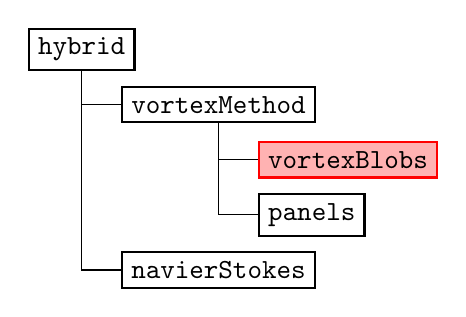
\begin{tikzpicture}[%
  grow via three points={one child at (0.5,-0.7) and
  two children at (0.5,-0.7) and (0.5,-1.4)},
  edge from parent path={(\tikzparentnode.south) |- (\tikzchildnode.west)}]
  \node {\texttt{hybrid}}
    child { node {\texttt{vortexMethod}}
    	child {node [selected] {\texttt{vortexBlobs}}}
    	child {node {\texttt{panels}}}  	
    }
    child [missing] {}				
    child [missing] {}				
    child { node {\texttt{navierStokes}}};
    %child { node [selected] {tex}
    %  child { node {generic}}
    %  child { node [optional] {latex}}
    %  child { node {plain}}
    %}
    %child [missing] {}
    %child { node {texdoc}};
\end{tikzpicture}
\end{figure}

\subsection*{Class structure:}
\begin{figure}[h]
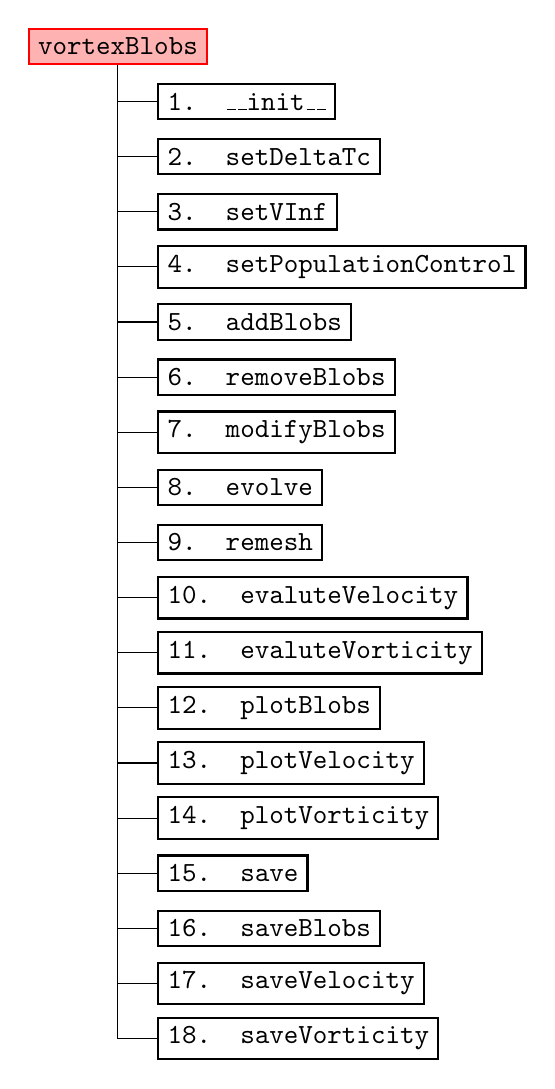
\begin{tikzpicture}[%
  grow via three points={one child at (0.5,-0.7) and
  two children at (0.5,-0.7) and (0.5,-1.4)},
  edge from parent path={(\tikzparentnode.south) |- (\tikzchildnode.west)}]
  \node [selected] {\texttt{vortexBlobs}}
    child { node {\texttt{1. \_\_init\_\_}}}
    child { node {\texttt{2. setDeltaTc}}}
    child { node {\texttt{3. setVInf}}}    
    child { node {\texttt{4. setPopulationControl}}}
    child { node {\texttt{5. addBlobs}}}
    child { node {\texttt{6. removeBlobs}}}    
    child { node {\texttt{7. modifyBlobs}}}    
    child { node {\texttt{8. evolve}}}    
    child { node {\texttt{9. remesh}}}    
    child { node {\texttt{10. evaluteVelocity}}}                    
    child { node {\texttt{11. evaluteVorticity}}}                        
    child { node {\texttt{12. plotBlobs}}}                        
    child { node {\texttt{13. plotVelocity}}}                        
    child { node {\texttt{14. plotVorticity}}}                            
    child { node {\texttt{15. save}}}                        
    child { node {\texttt{16. saveBlobs}}}                                        
    child { node {\texttt{17. saveVelocity}}}                                            
    child { node {\texttt{18. saveVorticity}}};
%    child { node [optional] {19. \texttt{\_generateBlobs}}}
%    child { node [optional] {20. \texttt{\_populationControl}}};        
        %child { node [selected] {tex}
    %  child { node {generic}}
    %  child { node [optional] {latex}}
    %  child { node {plain}}
    %}
    %child { node {texdoc}};
\end{tikzpicture}
\end{figure}

%\subsection*{Structure:}
%\begin{table}[h]
%\begin{tabular}{rl}
%	\texttt{vortexBlobs}: &  \\ \hline
%	-- & \texttt{\_\_init\_\_} \\
%	& \\
%	-- & \texttt{set\_deltaTc} \\ 
%	-- & \texttt{set\_popControlParameters} \\ 
%	-- & \texttt{addBlobs} \\ 
%	-- & \texttt{removeBlobs} \\ 
%	-- & \texttt{modifyBlobs} \\ 
%	-- & \texttt{evolve} \\ 
%	-- & \texttt{remesh} \\ 
%	-- & \texttt{evaluteVelocity} \\ 
%	-- & \texttt{evaluteVorticity} \\ 
%	-- & \texttt{plotBlobs} \\	
%	-- & \texttt{plotVelocity} \\
%	-- & \texttt{plotVorticity} \\
%	-- & \texttt{saveClass} \\ 
%	-- & \texttt{saveBlob} \\ 
%	-- & \texttt{saveVelocity} \\ 	
%	-- & \texttt{saveVorticity} \\ 
%	-- & \texttt{saveBlobPlot} \\ 
%	-- & \texttt{saveVelocityPlot} \\ 	
%	-- & \texttt{saveVorticityPlot} \\ 		
%	& \\
%	-- & \texttt{\_generateParticles} \\ 
%	-- & \texttt{\_popControl} \\
%\end{tabular}
%\end{table}

\newpage



\subsection{\texttt{\_\_init\_\_}}
	\paragraph{Description:} Initialize the \texttt{vortexBlobs} class with either the given input parameters or by a reading a \texttt{file} containing all the necessary parameters.\\
	
	\begin{tabular}{l|lp{7cm}}
		\multicolumn{2}{l}{\textbf{Input Parameters}} & \\ \hline
		\textit{File Name} & \multicolumn{2}{l}{Containing all the parameters to re-initalize the class.} \\ \cline{2-3}
		\multicolumn{3}{c}{--- or ---} \\ \cline{2-3}
		\multirow{4}{*}{\textit{Parameters}} & Vorticity Field &: \{\texttt{xBlob, yBlob, gBlob}\} or \{\texttt{wFunction, xBounds, yBounds}\}\\ \cline{2-3}
		& Blob parameters &: \texttt{overlap, h} \\ \cline{2-3}
		& Time Step parameters &: \texttt{deltaTc, nu, stepRedistribution, integrationMethod, computationMethod}\\ \cline{2-3}
		& Population control parameters &: \texttt{stepPopulationControl, gThreshold}\\ \cline{2-3}
	\end{tabular}\\
	
	\subsubsection*{Descriptions of the parameters:}
	\begin{tabular}{p{3.5cm}p{9cm}p{1cm}}
				\textit{Vorticity field} & & \textit{Default}\\ \hline
				\texttt{xBlob,yBlob} &:  the $x,y$ blob coordinates. & - \\
				\texttt{gBlob} &: the circulation $\Gamma_i$ associated to each of the vortex blobs. & - \\
				& & \\
				\multicolumn{2}{c}{\textit{--- or ---}} & \\
				& & \\
				\texttt{wExactFunction} &: the function that returns the exact value of vorticity $\omega$ at any given $x,y$ coordinates. &\\
				& 	\begin{tabular}{lp{10cm}}
						\textbf{Input parameters} &: \texttt{xEval,yEval}\\ 
						\textbf{Assigns} &: \texttt{-}\\ 			
						\textbf{Returns} &: \texttt{wEval}\\ 					
					\end{tabular} & - \\
				\texttt{xBounds, yBounds} &: the $x,y$ bounds of the domain where the particles was originally distributed. & - \\		 
	\end{tabular}\\
	\\ \\
	%	\begin{tabular}{lp{10cm}}
	%		\textbf{Input parameters} &: \texttt{xEval,yEval}\\ 
	%		\textbf{Assigns} &: \texttt{-}\\ 			
	%		\textbf{Returns} &: \texttt{vortEval}\\ 					
	%	\end{tabular}\\
	\begin{tabular}{p{3.5cm}p{9cm}p{1cm}}
				\multicolumn{2}{l}{\textit{Blob parameters}} & \textit{Default} \\ \hline				
				\texttt{overlap} &: the overlap ratio $h/\sigma$. & 1.0\\
				\texttt{h} &: the size of the cell $h$ associated to the blobs. \textit{Note:} Cells are square. & -\\
	\end{tabular}\\
	\\ \\
	\begin{tabular}{p{3.5cm}p{9cm}p{1cm}}
				\multicolumn{2}{l}{\textit{Time step parameters}} & \textit{Default}\\ \hline
				\texttt{deltaTc} &:  the size of the convective time step $\Delta t_c$. & - \\
				\texttt{nu} &: the fluid kinematic viscosity $\nu$, used to calculate the diffusion coefficient $c^2$ and diffusion time step size $\Delta T_d$.& - \\
				\texttt{stepRedistribution} &: the redistribution step frequency. & 1 \\
				\texttt{integrationMethod} &: the time integration method (\texttt{FE}: Forward euler , \texttt{RK4}: $4^{th}$ order Runge-Kutta). & RK4 \\
				\texttt{computationMethod} &: the calculation method to evolve the blobs, (\texttt{Direct}: Direct Method, \texttt{FMM}: Fast-Multipole Method) using (\texttt{CPU}, \texttt{GPU}). & \{FMM, GPU\}.\\
	\end{tabular}\\ 
    \\ \\ 
	\begin{tabular}{p{3.5cm}p{9cm}p{1cm}}
				\multicolumn{2}{l}{\textit{Population control parameters}} & \textit{Default} \\ \hline
				\texttt{stepPopulationControl} &: population control step frequency & 1.\\
				\texttt{gThreshold} &: the tuple with minimum \textbf{and} maximum value of the circulation $\Gamma_{min}$. & - \\
	\end{tabular}\\ 
    \\ \\  
	\begin{tabular}{p{3.5cm}p{9cm}p{1cm}}
				\multicolumn{2}{l}{\textit{Free stream velocity}} & \textit{Default}\\ \hline
				\texttt{vInf} &: The free-stream velocity function, returning the velocity action on the vortex blobs. & -\\		
				&		\begin{tabular}{lp{10cm}}
							\textbf{Input parameters} &: \texttt{t}\\ 
							\textbf{Assigns} &: \texttt{-}\\ 			
							\textbf{Returns} &: \texttt{vx,vy}\\ 					
						\end{tabular} & - \\
				
	\end{tabular}\\


\subsection{\texttt{setDeltaTc}}
	\paragraph{Description:} Function change the convective time step size $\Delta t_c$.\\
	
	 \begin{tabular}{p{3.5cm}p{10cm}p{1cm}}
				\multicolumn{2}{l}{\textit{Parameters}} & \textit{Default} \\ \hline
		   		\texttt{deltaTc} &: the new convection time step size $\Delta t_c$. & - \\
		\end{tabular} \vspace{5 mm}\\
	\\		
	\begin{tabular}{lp{10cm}}
		\textbf{Input parameters} &: \texttt{deltaTcNew}\\
		\textbf{Assigns} &:  \texttt{deltaTc}\\
		\textbf{Returns} &: \texttt{-}\\
	\end{tabular}

\subsection{\texttt{setPopulationControl}}
	\paragraph{Description:} function to modify the population control parameters.\\
	
	 \begin{tabular}{lp{10cm}}
				\textit{Parameters} & \\ \hline
		   		\texttt{gThresholdNew} &: the minimum and maximum circulation of the blobs, $\Gamma_{min}$\\
		   		\texttt{stepPopulationControlNew} &: the step number (frequency) of the population control.\\
		\end{tabular} \vspace{5 mm}\\
	\\		
	\begin{tabular}{lp{10cm}}
		\textbf{Input parameters} &: \texttt{gThresholdNew, stepPopulationControlNew}\\
		\textbf{Assigns} &:  \texttt{gThreshold, stepPopulationControl}\\
		\textbf{Returns} &: \texttt{-}\\
	\end{tabular}

		
\subsection{\texttt{addBlobs}}
	\paragraph{Description:} adds vortex particles by appending to the current set of particles.\\
	
	 \begin{tabular}{lp{10cm}}
				\textit{Parameters} & \\ \hline
		   		\texttt{xBlobNew,yBlobNew,gBlobNew} &: the coordinates and the strength of the new set of particles.\\
		\end{tabular} \vspace{5 mm}\\
	\\		
	\begin{tabular}{lp{10cm}}
		\textbf{Input parameters} &: \texttt{xBlobNew,yBlobNew,gBlobNew}\\
		\textbf{Assigns} &: \texttt{xBlob,yBlob,gBlob}\\
		\textbf{Returns} &: \texttt{-}\\
	\end{tabular}


\subsection{\texttt{removeBlobs}}
	\paragraph{Description:} removes vortex particles from the current set of particles. Using, the particle index, the associated $x,y$ and $\Gamma_i$ will be removed.\\
	
	 \begin{tabular}{lp{10cm}}
				\textit{Parameters} & \\ \hline
		   		\texttt{iBlob} &: the list of blob indices that is to be removed.\\
		\end{tabular} \vspace{5 mm}\\
	\\		
	\begin{tabular}{lp{10cm}}
		\textbf{Input parameters} &: \texttt{iBlob}\\
		\textbf{Assigns} &: \texttt{xBlob,yBlob,gBlob}\\
		\textbf{Returns} &: \texttt{-}\\
	\end{tabular}
	
	
\subsection{\texttt{modifyBlobs}}
	\paragraph{Description:} Replace the vortex particle strengths with the new strength.\\
	
	 \begin{tabular}{lp{10cm}}
				\textit{Parameters} & \\ \hline
		   		\texttt{iBlob} &: the list of blob indices that is to be modified.\\
		   		\texttt{gBlobNew} &: the new strength of the blobs.\\		   		
		\end{tabular} \vspace{5 mm}\\
	\\		
	\begin{tabular}{lp{10cm}}
		\textbf{Input parameters} &: \texttt{iBlob,gBlobNew}\\
		\textbf{Assigns} &: \texttt{gBlob}\\
		\textbf{Returns} &: \texttt{-}\\
	\end{tabular}	

\subsection{\texttt{evolve}}
	\paragraph{Description:} Evolves the vortex blobs according to the \texttt{\_\_init\_\_} definition. The \texttt{evolve} function, knows when (has a counter) to redistribute and perform population control. Depending on the diffusion time step $\Delta t_d$, the evolve function will also perform the diffusion process (modified interpolation).\\
	
	 \begin{tabular}{lp{10cm}}
				\textit{Parameters} & \\ \hline
		   		\texttt{xBlobNew,yBlobNew,gBlobNew} &: the new set of particle after the evolution process.\\
		\end{tabular} \vspace{5 mm}\\
	\\		
	\begin{tabular}{lp{10cm}}
		\textbf{Input parameters} &: \texttt{-}\\
		\textbf{Assigns} &: \texttt{xBlob,yBlob,gBlob}\\	
		\textbf{Returns} &: \texttt{-}\\
	\end{tabular}			


\subsection{\texttt{remesh}}
	\paragraph{Description:}  Function to remesh the particles on to the remeshing grid. When $c=0$, the remeshing will be done without diffusion. If $c>0$, the modified interpolation will perform the diffusion.
	\\
	\\		
	\begin{tabular}{lp{10cm}}
		\textbf{Input parameters} &: \texttt{c}\\ 
		\textbf{Assigns} &: \texttt{xBlob,yBlob,wBlob}\\ 			
		\textbf{Returns} &: \texttt{-}\\ 					
	\end{tabular}


\subsection{\texttt{evaluateVelocity}}
	\paragraph{Description:} Function to evaluate the total induced velocity due to the blobs, and the external velocity at a given target locations.\\
	
	    \begin{tabular}{lp{10cm}}
			\textit{Parameters} & \\ \hline
			 \texttt{xTarget,yTarget} &: the $x,y$ coordinate of the target location, where the total velocity is to be evaluated.\\
			\texttt{vxTarget,vyTarget} &: the $x,y$ induced velocity at the target points in global coordinate system.\\
		\end{tabular} \vspace{5 mm}
	\\		
	\begin{tabular}{lp{10cm}}
		\textbf{Input parameters} &: \texttt{xTarget,yTarget}\\ 
		\textbf{Assigns} &: \texttt{-}\\ 			
		\textbf{Returns} &: \texttt{vxTarget,vyTarget}\\ 					
	\end{tabular}	

\subsection{\texttt{evaluateVorticity}}
	\paragraph{Description:} Function to evaluate the total induced vorticity due to the blobs, and the external velocity at a given target coordinates.\\
	
	    \begin{tabular}{lp{10cm}}
			\textit{Parameters} & \\ \hline
			 \texttt{xTarget,yTarget} &: the $x,y$ coordinate of the target location, where the total velocity is to be evaluated.\\
			\texttt{wTarget} &: the $x,y$ induced vorticity at the target points in global coordinate system.\\
		\end{tabular} \vspace{5 mm}
	\\		
	\begin{tabular}{lp{10cm}}
		\textbf{Input parameters} &: \texttt{xTarget,yTarget}\\ 
		\textbf{Assigns} &: \texttt{-}\\ 			
		\textbf{Returns} &: \texttt{wTarget}\\ 					
	\end{tabular}


		
\subsection{plots \ldots}
	\paragraph{Description:} functions to plot and/or save all the results in a given region. The data should be store for scientific visualization (paraview format)\\
	
		\begin{tabular}{lp{10cm}}
			\textit{Plot variables:} & \\ \hline
			\texttt{plotBlob} &: plot the coordinates and the circulation of the blobs.\\
			\texttt{plotVelocity} &: plot the velocity field.\\ 
			\texttt{plotVorticity} &: plot the vorticity field.\\ 
		\end{tabular} \vspace{5 mm}
		
		\begin{tabular}{lp{10cm}}
			\textit{Parameters:} & \\ \hline
			\texttt{xBounds,yBounds} &: $x,y$ bounds of the grid, where the data is to be evaluated.\\ 
			\texttt{nGrid} &: $x,y$ number of grid points.\\
		\end{tabular} \vspace{5 mm}\\
	\\
	\begin{tabular}{lp{10cm}}
		\textbf{Input parameters} &: \texttt{xBounds,yBounds,nGrid}\\
		\textbf{Assigns} &: \texttt{-}\\ 			
		\textbf{Returns} &: \texttt{figureHandle} or \texttt{.pvd}\\ 					
	\end{tabular}	

\subsection{save data \ldots}
	\paragraph{Description:} functions to save the data. The data file will be in compressed, binary format to store efficiently.\\

		\begin{tabular}{lp{10cm}}
			\textit{Save variables:} & \\ \hline
			\texttt{save} &: all the data of the \texttt{vortexBlob} class is saved. This can be used later to restart the problem, i.e the parameter to init the problem.\\
			\texttt{saveBlobs} &: the function to save the blob data at the current time instant. List of numpy array.\\ 			
			\texttt{saveVelocity} &: save the velocity field of a given region or a given set of points.\\ 
			\texttt{saveVorticity} &: save the vorticity field of the given region or the given set of points.\\ 
		\end{tabular} \vspace{5 mm}
	
		\begin{tabular}{lp{10cm}}
			\textit{Parameters:} & \\ \hline
			\texttt{xBounds,yBounds} &: $x,y$ bounds of the grid, where the data is to be evaluated and saved.\\ 
			\texttt{nGrid} &: $x,y$ number of grid points.\\
			\texttt{xEval,yEval} &: $x,y$ coordinates of the location where the data is to be evaluated and saved.\\ 
		\end{tabular} \vspace{5 mm}\\
	\\
	\begin{tabular}{lp{10cm}}
		\textbf{Input parameters} &: \texttt{xBounds,yBounds,hGrid} or \texttt{xEval,yEval}\\ 
		\textbf{Assigns} &: \texttt{-}\\ 			
		\textbf{Returns} &: \texttt{.npz, .bin or similar}\\ 					
	\end{tabular}



%\subsection{save plots \ldots}
%	\paragraph{Description:} Function to save the plots as scientific visualization format \texttt{.pvd}.\\
%	
%		\begin{tabular}{lp{10cm}}
%			\textit{Save variables:} & \\ \hline
%			\texttt{saveBlobPlot} &: save the particle position and strengths as glyphs.\\
%			\texttt{saveVelocityPlot} &: save the velocity plot of a given region.\\ 
%			\texttt{saveVorticityPlot} &: save the vorticity of a given region.\\ 
%		\end{tabular} \vspace{5 mm}
%		
%		\begin{tabular}{lp{10cm}}
%			\textit{Parameters:} & \\ \hline
%			\texttt{xBounds,yBounds} &: $x,y$ bounds of the grid, where the data is to be evaluated and saved.\\ 
%			\texttt{hGrid} &: $x,y$ spacing of the evaluation grid.\\
%		\end{tabular} \vspace{5 mm}\\
%	\\
%	\begin{tabular}{lp{10cm}}
%		\textbf{Input parameters} &: \texttt{xBounds,yBounds,hGrid}\\
%		\textbf{Assigns} &: \texttt{-}\\ 			
%		\textbf{Returns} &: \texttt{.pvd}\\ 					
%	\end{tabular}
	


%\subsection{\texttt{\_generateParticles}}
%	\paragraph{Description:} \textit{Internal} function to generate/initialize the particles.\\
%	\\
%	\\
%		\begin{tabular}{lp{10cm}}
%			\textbf{Input parameters} &: \texttt{wExactFunction, xBounds, yBounds}\\ 
%			\textbf{Assigns} &: \texttt{xBlob,yBlob,wBlob}\\ 			
%			\textbf{Returns} &: \texttt{-}\\ 					
%		\end{tabular}	
%
%
%\subsection{\texttt{\_popControl}}
%	\paragraph{Description:} \textit{Internal} function to perform population control on the current set of particles.\\
%	\\
%	\\	
%		\begin{tabular}{lp{10cm}}
%			\textbf{Input parameters} &: \texttt{-}\\ 
%			\textbf{Assigns} &: \texttt{xBlob,yBlob,wBlob}\\ 			
%			\textbf{Returns} &: \texttt{-}\\ 					
%		\end{tabular}	
%\section{\texttt{panels}}
The main structure of the panel method class \texttt{panels}. This class contains all the functions related to the calculation of panels.

\begin{figure}[h]
\centering
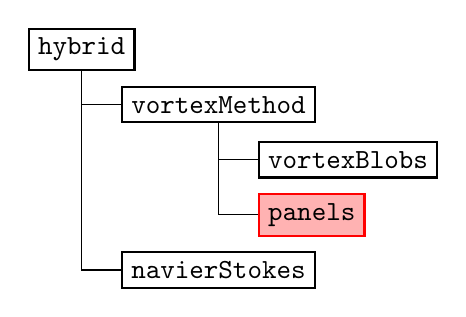
\begin{tikzpicture}[%
  grow via three points={one child at (0.5,-0.7) and
  two children at (0.5,-0.7) and (0.5,-1.4)},
  edge from parent path={(\tikzparentnode.south) |- (\tikzchildnode.west)}]
  \node {\texttt{hybrid}}
    child { node {\texttt{vortexMethod}}
    	child {node {\texttt{vortexBlobs}}}
    	child {node [selected] {\texttt{panels}}}  	
    }
    child [missing] {}				
    child [missing] {}				
    child { node {\texttt{navierStokes}}};
    %child { node [selected] {tex}
    %  child { node {generic}}
    %  child { node [optional] {latex}}
    %  child { node {plain}}
    %}
    %child [missing] {}
    %child { node {texdoc}};
\end{tikzpicture}
\end{figure}


\subsection*{Class structure:}
\begin{figure}[h]
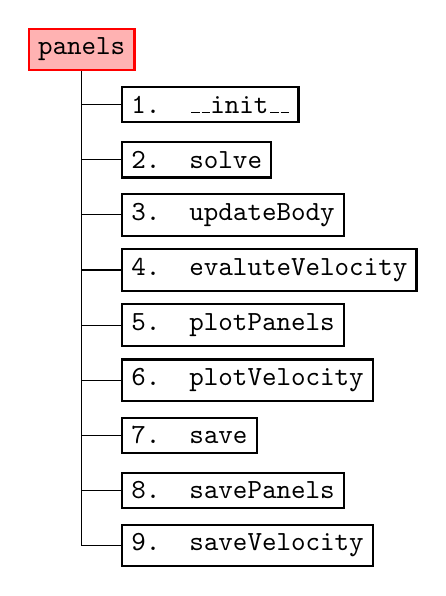
\begin{tikzpicture}[%
  grow via three points={one child at (0.5,-0.7) and
  two children at (0.5,-0.7) and (0.5,-1.4)},
  edge from parent path={(\tikzparentnode.south) |- (\tikzchildnode.west)}]
  \node [selected] {\texttt{panels}}
    child { node {\texttt{1. \_\_init\_\_}}}
    child { node {\texttt{2. solve}}}
    child { node {\texttt{3. updateBody}}}    
    child { node {\texttt{4. evaluteVelocity}}}                    
    child { node {\texttt{5. plotPanels}}}                        
    child { node {\texttt{6. plotVelocity}}}                        
    child { node {\texttt{7. save}}}                        
    child { node {\texttt{8. savePanels}}}                                        
    child { node {\texttt{9. saveVelocity}}};                                            
	%  child { node [selected] {tex}
    %  child { node {generic}}
    %  child { node [optional] {latex}}
    %  child { node {plain}}
    %}
    %child { node {texdoc}};
\end{tikzpicture}
\end{figure}

\subsection{\texttt{\_\_init\_\_}}
	\begin{tabular}{l|lp{7cm}}
		\multicolumn{2}{l}{\textbf{Input Parameters}} & \\ \hline
		\textit{File Name} & \multicolumn{2}{l}{Containing all the parameters to re-initalize the class.} \\ \hline
		\multirow{2}{*}{\textit{Parameters}} & Panel coordinates &: \{\texttt{xCP, yCP, xPanel, yPanel, cmGlobal, thetaLocal}\}\\ \cline{2-3}
		& External velocity &: \texttt{externVel} \\ \cline{2-3}
	\end{tabular}
	\paragraph{Description:} Initialize the \texttt{panels} class with the given input parameters. In the case of a multibody problem, a list of panel coordinates can be given and internally it takes care of the inter-coupling.\\
	\\
	\begin{tabular}{lp{10cm}}
				\textit{Panel coordinates} & \\ \hline
				\texttt{xCP,yCP} &:  the local $x,y$-coordinates of the panel collocation points.\\ 
				\texttt{xPanel,yPanel} &: the local coordinate of the panel edges. \textit{Note}: Should have a closed loop (end with initial point coordinates).\\ 
				\texttt{cmGlobal} &:  the position of reference points of a given panel body.\\
				\texttt{thetaLocal} &:  the rotational angles of the panel body axes w.r.t to the global $x$-axis.\\
	\end{tabular}\\ 
    \\ \\
	\begin{tabular}{lp{10cm}}
				\textit{External velocity} & \\ \hline
				\texttt{externVel} &:  Reference to an external velocity \textbf{function} acting of the panels. For the panel case, the external velocity will the induced velocity of the blobs + freestream \texttt{vortexBlob.evaluateVelocity}.\\
	\end{tabular}\\
	
		\begin{tabular}{lp{10cm}}
			\textbf{Input parameters} &: \texttt{xCP,yCP}\\ 
			\textbf{Assigns} &: \texttt{-}\\ 			
			\textbf{Returns} &: \texttt{vxCP,vyCP}\\ 					
		\end{tabular}\\

		
\subsection{\texttt{solve}}
	\paragraph{Description:} Function to solve the panel strength to satisfy no-slip condition.\\
	
		\begin{tabular}{lp{10cm}}
			\textit{Parameters} & \\ \hline
			\texttt{sPanel} &: the new strength of the panels, satisfying the no-through b.c of the body (no-slip with vortex panels.).\\
		\end{tabular} \vspace{5 mm}
		\\		
		\begin{tabular}{lp{10cm}}
			\textbf{Input parameters} &: \texttt{-}\\ 
			\textbf{Assigns} &: \texttt{sPanel}\\ 			
			\textbf{Returns} &: \texttt{-}\\ 					
		\end{tabular}		
			
		
\subsection{\texttt{updateBody}}
	\paragraph{Description:} Function to update all the panel body coordinates. This function will internally calculate the new panel coordinates \texttt{xPanel,yPanel,xCP,yCP} and rebuild the inter-induction matrix \texttt{A}.\\
	
		\begin{tabular}{lp{10cm}}
			\textit{Parameters} & \\ \hline
			\texttt{xPanel,yPanel} &: the $x,y$ panel coordinates in global.\\
			\texttt{xCP,yCP} &: the $x,y$ coordinates of the collocation point in global.\\
			\texttt{A} &: the panel self-induction matrix.
		\end{tabular} \vspace{5 mm}
		\\		
		\begin{tabular}{lp{10cm}}
			\textbf{Input parameters} &: \texttt{thetaLocals,cmGlobals}\\ 
			\textbf{Assigns} &: \texttt{A, xPanel, yPanel, xCP, yCP}\\ 			
			\textbf{Returns} &: \texttt{-}\\ 					
		\end{tabular}	

\subsection{\texttt{evaluateVelocity}}
	\paragraph{Description:} Function to evaluate the total induced velocity due to the panels and free-stream velocity (\textit{optional}).\\
	
	    \begin{tabular}{lp{10cm}}
			\textit{Parameters} & \\ \hline
			 \texttt{xTarget,yTarget} &: the $x,y$ coordinate of the target location, where the total velocity is to be evaluated.\\
			\texttt{vxTarget,vyTarget} &: the $x,y$ induced velocity of the target points in global coordinate system.\\
		\end{tabular} \vspace{5 mm}
	\\		
	\begin{tabular}{lp{10cm}}
		\textbf{Input parameters} &: \texttt{xTarget,yTarget}\\ 
		\textbf{Assigns} &: \texttt{-}\\ 			
		\textbf{Returns} &: \texttt{vxTarget,vyTarget}\\ 					
	\end{tabular}					

		
\subsection{plots \ldots}
	\paragraph{Description:} Function to plot and save (\textit{optional}) all the results in a given region or set of points.\\
	
		\begin{tabular}{lp{10cm}}
			\textit{Plot variables:} & \\ \hline
			\texttt{plotPanels} &:plot the panel coordinates at the current time instant.\\
			\texttt{plotVelocity} &: plot the velocity field.\\ 
			\texttt{plotVorticity} &: plot the vorticity field.\\ 
		\end{tabular} \vspace{5 mm}
		
		\begin{tabular}{lp{10cm}}
			\textit{Parameters:} & \\ \hline
			\texttt{xBounds,yBounds} &: $x,y$ bounds of the grid, where the data is to be evaluated and saved.\\ 
			\texttt{nGrid} &: $x,y$ number of evaluation grid points.\\ 
			\texttt{xEval,yEval} &: $x,y$ coordinates of the location where the data is to be evaluated and saved.\\ 
		\end{tabular} \vspace{5 mm}\\
	\\
	\begin{tabular}{lp{10cm}}
		\textbf{Input parameters} &: \texttt{xBounds,yBounds,hGrid} or \texttt{xEval,yEval}\\ 
		\textbf{Assigns} &: \texttt{-}\\ 			
		\textbf{Returns} &: \texttt{figureHandle} and/or \texttt{.pvd}\\ 					
	\end{tabular}	

\subsection{save data \ldots}
	\paragraph{Description:} Function to save the data in a given region or at given set of points.\\

		\begin{tabular}{lp{10cm}}
			\textit{Save variables:} & \\ \hline
			\texttt{save} &: all the data of the \texttt{panels} class, to be used to restart later.\\ 			
			\texttt{savePanels} &: the function to save the panel data at the current time instant.\\ 			
			\texttt{saveVelocity} &: save the velocity field of the given region or the given set of points.\\ 
			\texttt{saveVorticity} &: save the vorticity field of the given region or the given set of points.\\ 
		\end{tabular} \vspace{5 mm}
	
		\begin{tabular}{lp{10cm}}
			\textit{Parameters:} & \\ \hline
			\texttt{xBounds,yBounds} &: $x,y$ bounds of the grid, where the data is to be evaluated and saved.\\ 
			\texttt{nGrid} &: $x,y$ number of grid points.\\ 
			\texttt{xEval,yEval} &: $x,y$ coordinates of the location where the data is the be evaluated and saved.\\ 
		\end{tabular} \vspace{5 mm}\\
	\\
	\begin{tabular}{lp{10cm}}
		\textbf{Input parameters} &: \texttt{xBounds,yBounds,hGrid} or \texttt{xEval,yEval}\\ 
		\textbf{Assigns} &: \texttt{-}\\ 			
		\textbf{Returns} &: \texttt{.npz}\\ 					
	\end{tabular}

%
%
%\subsection{save plots \ldots}
%	\paragraph{Description:} Function to save the plots of a region or a given set of points as scientific visualization format \texttt{.pvd}.\\
%	
%		\begin{tabular}{lp{10cm}}
%			\textit{Save variables:} & \\ \hline
%			\texttt{saveVelocityPlot} &: save the velocity $\mathbf{V}$ plot.\\ 
%			\texttt{saveVorticityPlot} &: save the vorticity $\mathbf{\omega}$ plot.\\ 
%		\end{tabular} \vspace{5 mm}
%		
%		\begin{tabular}{lp{10cm}}
%			\textit{Parameters:} & \\ \hline
%			\texttt{xBounds,yBounds} &: $x,y$ bounds of the grid, where the data is to be evaluated and saved.\\ 
%			\texttt{hGrid} &: $x,y$ spacing of the evaluation grid.\\ 
%			\texttt{xEval,yEval} &: $x,y$ coordinates of the location where the data is the be evaluated and saved.\\ 
%		\end{tabular} \vspace{5 mm}\\
%	\\
%	\begin{tabular}{lp{10cm}}
%		\textbf{Input parameters} &: \texttt{xBounds,yBounds,hGrid} or \texttt{xEval,yEval} \\ 
%		\textbf{Assigns} &: \texttt{-}\\ 			
%		\textbf{Returns} &: \texttt{.pvd}\\ 					
%	\end{tabular}
%\section{\texttt{vortexMethod}}
The main structure of the \texttt{vortexBlobs} + \texttt{panels} (vortexMethod) class. This class contains all the function related to the calculations of panel with vortex blobs.

\begin{figure}[h]
\centering
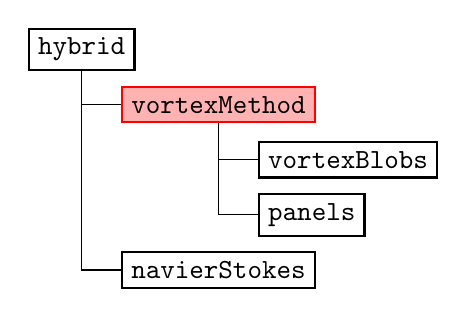
\begin{tikzpicture}[%
  grow via three points={one child at (0.5,-0.7) and
  two children at (0.5,-0.7) and (0.5,-1.4)},
  edge from parent path={(\tikzparentnode.south) |- (\tikzchildnode.west)}]
  \node {\texttt{hybrid}}
    child { node [selected] {\texttt{vortexMethod}}
    	child {node {\texttt{vortexBlobs}}}
    	child {node {\texttt{panels}}}  	
    }
    child [missing] {}				
    child [missing] {}				
    child { node {\texttt{navierStokes}}};
    %child { node [selected] {tex}
    %  child { node {generic}}
    %  child { node [optional] {latex}}
    %  child { node {plain}}
    %}
    %child [missing] {}
    %child { node {texdoc}};
\end{tikzpicture}
\end{figure}

\subsection*{Class structure:}
\begin{figure}[h]
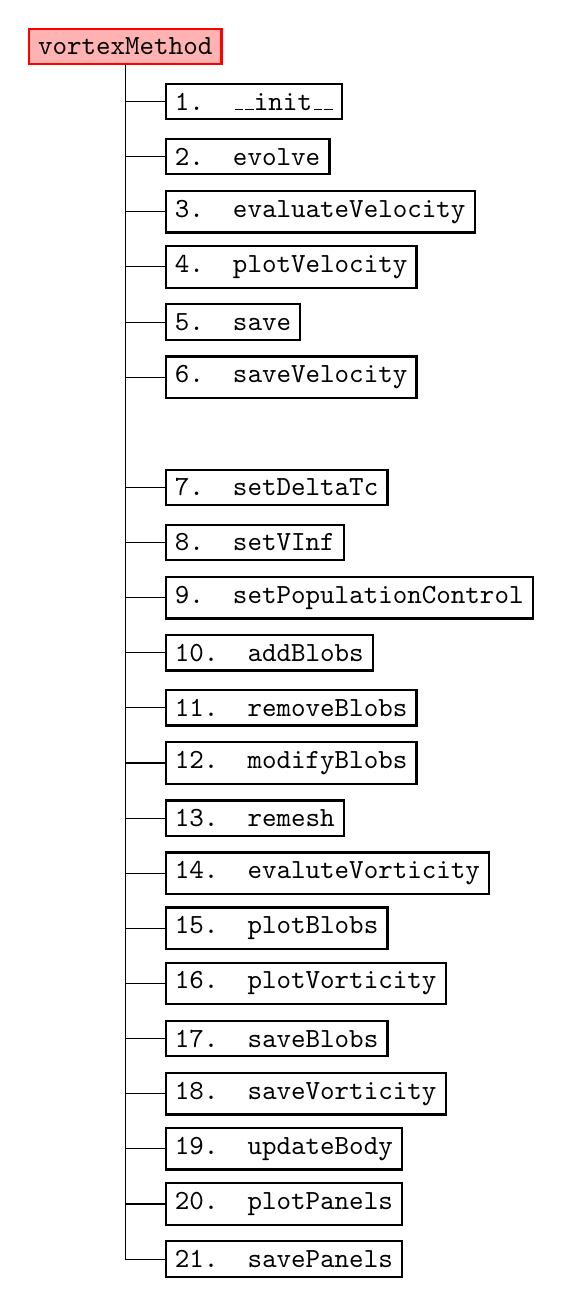
\begin{tikzpicture}[%
  grow via three points={one child at (0.5,-0.7) and
  two children at (0.5,-0.7) and (0.5,-1.4)},
  edge from parent path={(\tikzparentnode.south) |- (\tikzchildnode.west)}]
  \node [selected] {\texttt{vortexMethod}}
    child { node {\texttt{1. \_\_init\_\_}}}
    child { node {\texttt{2. evolve}}}
    child { node {\texttt{3. evaluateVelocity}}}
    child { node {\texttt{4. plotVelocity}}}                        
    child { node {\texttt{5. save}}}                        
    child { node {\texttt{6. saveVelocity}}}                                            
    child [missing] {}
    child { node {\texttt{7. setDeltaTc}}}
    child { node {\texttt{8. setVInf}}}    
    child { node {\texttt{9. setPopulationControl}}}
    child { node {\texttt{10. addBlobs}}}
    child { node {\texttt{11. removeBlobs}}}    
    child { node {\texttt{12. modifyBlobs}}}    
    child { node {\texttt{13. remesh}}}    
    child { node {\texttt{14. evaluteVorticity}}}                        
    child { node {\texttt{15. plotBlobs}}}                        
    child { node {\texttt{16. plotVorticity}}}                            
    child { node {\texttt{17. saveBlobs}}}                                        
    child { node {\texttt{18. saveVorticity}}}
    child { node {\texttt{19. updateBody}}}    
    child { node {\texttt{20. plotPanels}}}                        
    child { node {\texttt{21. savePanels}}};                                        
    	             
%    child { node {\texttt{5. plotPanels}}}                        
%    child { node {\texttt{6. plotVelocity}}}                        
%    child { node {\texttt{7. save}}}                        
%    child { node {\texttt{8. savePanels}}}                                        
%    child { node {\texttt{9. saveVelocity}}};                                            
	%  child { node [selected] {tex}
    %  child { node {generic}}
    %  child { node [optional] {latex}}
    %  child { node {plain}}
    %}
    %child { node {texdoc}};
\end{tikzpicture}
\end{figure}

%
%
%\subsection*{Class structure:}
%\begin{table}[h]
%\begin{tabular}{rl}
%	\texttt{vortexMethod}: &  \\ \hline
%	-- & \texttt{\_\_init\_\_} \\
%	& \\
%	-- & \texttt{evolve} \\ 
%	-- & \texttt{evaluateVelocity} \\ 
%	-- & \texttt{plotBlobsPanels} \\ 	
%	-- & \texttt{plotVelocity} \\ 
%	-- & \texttt{plotVorticity} \\ 	
%	-- & \texttt{saveClass} \\ 
%	-- & \texttt{saveVelocity} \\ 
%	-- & \texttt{saveVorticity} \\ 
%	-- & \texttt{saveVelocityPlot} \\ 
%	-- & \texttt{saveVorticityPlot} \\ 	
%\end{tabular}
%%\caption{\texttt{vortexMethod} class structure}
%\end{table}

\subsection{\texttt{\_\_init\_\_}}
	\begin{tabular}{l|lp{7cm}}
		\multicolumn{2}{l}{\textbf{Input Parameters}} & \\ \hline
		\textit{File Name} & \multicolumn{2}{l}{Containing all the parameters to re-initalize the class.} \\ \hline
		\multirow{2}{*}{\textit{Parameters}} & \texttt{vortexBlobs} &: \{\texttt{vortexBlobs}\} class. \\ \cline{2-3}
		& \texttt{panels} &: \texttt{panels} class. \\ \cline{2-3}
	\end{tabular}
	\paragraph{Description:} Initialize the \texttt{vortexMethod} class using \textbf{vortexBlob}+\textbf{panelMethod} classes.
	\paragraph{Input parameters:}
	\begin{list}{\quad}{}
	\item \texttt{vortexBlob}: vortex particle class
	\item \texttt{panelMethod}: panel method class				
	\end{list}

\subsection{\texttt{evolve}}
	\paragraph{Description:} Function to evolve (i.e. step) the vortex and panel together. All the necessary parameters are preassigned during the init of the vortex and panel class.\\
	
	    \begin{tabular}{lp{10cm}}
			\textit{Parameters:} & \\ \hline
			 \texttt{xBlobNew,yBlobNew,gBlobNew} &: the new $x,y$ coordinate and the new circulation $\Gamma_i$ of the blob at the new time instant.\\
			\texttt{xPanelNew,yPanelNew,sPanelNew} &: the new $x,y$ coordinates of the panel and its new strength at the new time instant.\\
		\end{tabular} \vspace{5 mm}
	\\		
	\begin{tabular}{lp{10cm}}
		\textbf{Input parameters} &: \texttt{-}\\ 
		\textbf{Assigns} &: \texttt{xBlob,yBlob,gBlob,xPanel,yPanel,sPanel}\\ 			
		\textbf{Returns} &: \texttt{-}\\ 					
	\end{tabular}

\subsection{\texttt{evaluateVelocity}}
	\paragraph{Description:} Function to evaluate the total induced velocity due to the vortex blobs, panels, and the external velocity at a given target coordinates.\\
	
	    \begin{tabular}{lp{10cm}}
			\textit{Parameters} & \\ \hline
			 \texttt{xTarget,yTarget} &: the $x,y$ coordinate of the target location, where the total velocity is to be evaluated.\\
			\texttt{vxTarget,vyTarget} &: the $x,y$ induced velocity of the target points in global coordinate system.\\
		\end{tabular} \vspace{5 mm}
	\\		
	\begin{tabular}{lp{10cm}}
		\textbf{Input parameters} &: \texttt{xTarget,yTarget}\\ 
		\textbf{Assigns} &: \texttt{-}\\ 			
		\textbf{Returns} &: \texttt{vxTarget,vyTarget}\\ 					
	\end{tabular}
		
\subsection{plots \ldots}
	\paragraph{Description:} Function to plot and save (\textit{optional}) all the results in a given region or set of points.\\
	
		\begin{tabular}{lp{10cm}}
			\textit{Plot variables:} & \\ \hline
			\texttt{plotBlobs/plotPanels} &: the plot of blobs and the panel coordinates.\\
			\texttt{plotVelocity} &: plot the velocity field of the region of the given set of points.\\ 
			\texttt{plotVorticity} &: plot the vorticity field.\\ 
		\end{tabular} \vspace{5 mm}
		
		\begin{tabular}{lp{10cm}}
			\textit{Parameters:} & \\ \hline
			\texttt{xBounds,yBounds} &: $x,y$ bounds of the grid, where the data is to be evaluated and saved.\\ 
			\texttt{nGrid} &: $x,y$ number of grid points.\\ 
			\texttt{xEval,yEval} &: $x,y$ coordinates of the location where the data is the be evaluated and saved.\\ 
		\end{tabular} \vspace{5 mm}\\
	\\
	\begin{tabular}{lp{10cm}}
		\textbf{Input parameters} &: \texttt{xBounds,yBounds,nGrid} or \texttt{xEval,yEval}\\ 
		\textbf{Assigns} &: \texttt{-}\\ 			
		\textbf{Returns} &: \texttt{figureHandle} or \texttt{saveFile}\\ 					
	\end{tabular}						

\subsection{save data \ldots}
	\paragraph{Description:} Function to save the data in a given region or at given set of points.\\

		\begin{tabular}{lp{10cm}}
			\textit{Save variables:} & \\ \hline
			\texttt{save} &: all the data of the \texttt{vortexMethod} class, to be used to restart later.\\ 			
			\texttt{saveBlobs/savePanels} &: the function to save the blobs and panel data at the current time instant.\\ 			
			\texttt{saveVelocity} &: the velocity field.\\ 
			\texttt{saveVorticity} &: the vorticity field.\\ 
		\end{tabular} \vspace{5 mm}
	
		\begin{tabular}{lp{10cm}}
			\textit{Parameters:} & \\ \hline
			\texttt{xBounds,yBounds} &: $x,y$ bounds of the grid, where the data is to be evaluated and saved.\\ 
			\texttt{nGrid} &: $x,y$ number of grid points.\\ 
			\texttt{xEval,yEval} &: $x,y$ coordinates of the location where the data is the be evaluated and saved.\\ 
		\end{tabular} \vspace{5 mm}\\
	\\
	\begin{tabular}{lp{10cm}}
		\textbf{Input parameters} &: \texttt{xBounds,yBounds,nGrid} or \texttt{xEval,yEval}\\ 
		\textbf{Assigns} &: \texttt{-}\\ 			
		\textbf{Returns} &: \texttt{.npz}\\ 					
	\end{tabular}

%\subsection{save plots \ldots}
%	\paragraph{Description:} Function to save the plots of a region or a given set of points as scientific visualization format \texttt{.pvd}.\\
%	
%		\begin{tabular}{lp{10cm}}
%			\textit{Save variables:} & \\ \hline
%			\texttt{saveVelocityPlot} &: save the velocity $\mathbf{V}$ plot.\\ 
%			\texttt{saveVorticityPlot} &: save the vorticity $\mathbf{\omega}$ plot.\\ 
%		\end{tabular} \vspace{5 mm}
%		
%		\begin{tabular}{lp{10cm}}
%			\textit{Parameters:} & \\ \hline
%			\texttt{xBounds,yBounds} &: $x,y$ bounds of the grid, where the data is to be evaluated and saved.\\ 
%			\texttt{hGrid} &: $x,y$ spacing of the evaluation grid.\\ 
%			\texttt{xEval,yEval} &: $x,y$ coordinates of the location where the data is the be evaluated and saved.\\ 
%		\end{tabular} \vspace{5 mm}\\
%	\\
%	\begin{tabular}{lp{10cm}}
%		\textbf{Input parameters} &: \texttt{xBounds,yBounds,hGrid} or \texttt{xEval,yEval} \\ 
%		\textbf{Assigns} &: \texttt{-}\\ 			
%		\textbf{Returns} &: \texttt{.pvd}\\ 					
%	\end{tabular}
%\section{\texttt{navierStokes}}
The main structure for the Navier-stokes class \texttt{navierStokes}. This class contains all the functions related to computation of the Navier-stokes problem. Below is set of functions that acts as the interface to the class.

\begin{figure}[h]
\centering
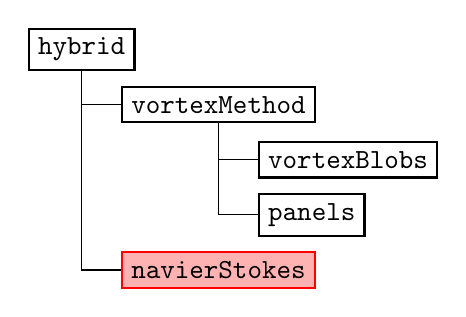
\begin{tikzpicture}[%
  grow via three points={one child at (0.5,-0.7) and
  two children at (0.5,-0.7) and (0.5,-1.4)},
  edge from parent path={(\tikzparentnode.south) |- (\tikzchildnode.west)}]
  \node {\texttt{hybrid}}
    child { node {\texttt{vortexMethod}}
    	child {node {\texttt{vortexBlobs}}}
    	child {node {\texttt{panels}}}  	
    }
    child [missing] {}				
    child [missing] {}				
    child { node [selected] {\texttt{navierStokes}}};
    %child { node [selected] {tex}
    %  child { node {generic}}
    %  child { node [optional] {latex}}
    %  child { node {plain}}
    %}
    %child [missing] {}
    %child { node {texdoc}};
\end{tikzpicture}
\end{figure}


\subsection*{Class structure:}
\begin{figure}[h]
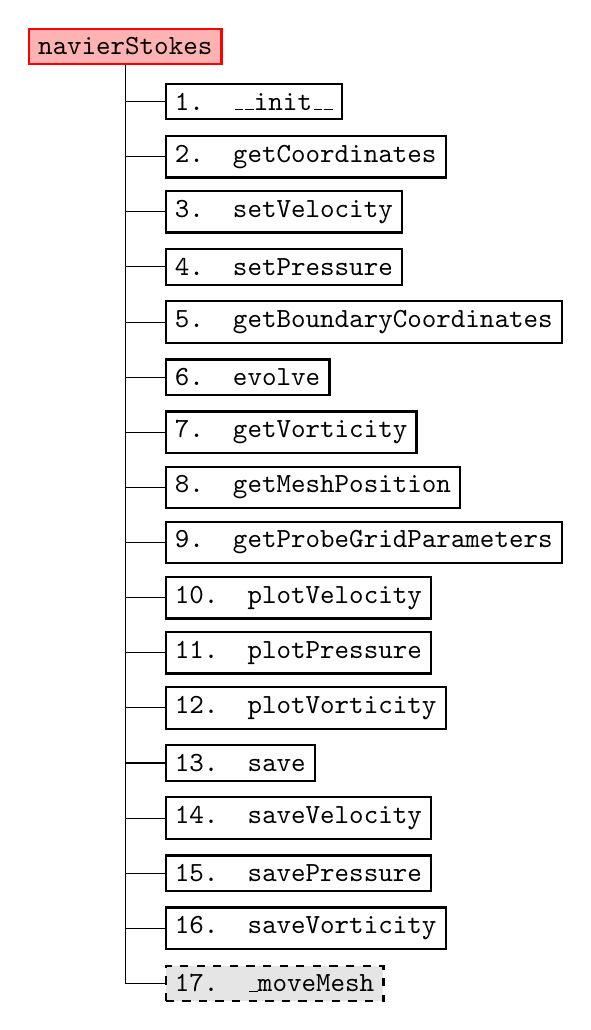
\begin{tikzpicture}[%
  grow via three points={one child at (0.5,-0.7) and
  two children at (0.5,-0.7) and (0.5,-1.4)},
  edge from parent path={(\tikzparentnode.south) |- (\tikzchildnode.west)}]
  \node [selected] {\texttt{navierStokes}}
    child { node {\texttt{1. \_\_init\_\_}}}
    child {node  {\texttt{2. getCoordinates}}}
    child { node {\texttt{3. setVelocity}}}
    child { node {\texttt{4. setPressure}}}
    child { node {\texttt{5. getBoundaryCoordinates}}}                        
    child { node {\texttt{6. evolve}}}
    child { node {\texttt{7. getVorticity}}}                        
    child { node {\texttt{8. getMeshPosition}}}                        
    child { node {\texttt{9. getProbeGridParameters}}}                        
    child { node {\texttt{10. plotVelocity}}}                        
    child { node {\texttt{11. plotPressure}}}                        
    child { node {\texttt{12. plotVorticity}}}                        
    child { node {\texttt{13. save}}}                        
    child { node {\texttt{14. saveVelocity}}}                                            
    child { node {\texttt{15. savePressure}}}                                            
    child { node {\texttt{16. saveVorticity}}}
    child { node [optional]{\texttt{17. \_moveMesh}}};
	%  child { node [selected] {tex}
    %  child { node {generic}}
    %  child { node [optional] {latex}}
    %  child { node {plain}}
    %}
    %child { node {texdoc}};
\end{tikzpicture}
\end{figure}

%\subsection*{Class structure:}
%\begin{table}[h]
%\begin{tabular}{rl}
%	\texttt{navierStokes}: &  \\ \hline
%	-- & \texttt{\_\_init\_\_} \\
%	& \\
%	-- & \texttt{initialConditions} \\ 
%	-- & \texttt{evolve} \\ 
%	-- & \texttt{boundaryCoordinates} \\ 
%	-- & \texttt{updateMesh} \\ 
%	-- & \texttt{moveMesh} \\ 
%	-- & \texttt{computeVorticity} \\ 
%	-- & \texttt{meshPosition}\\
%	-- & \texttt{probeGridParameters} \\ 	
%	-- & \texttt{plotVelocity} \\ 		
%	-- & \texttt{plotPressure} \\ 		
%	-- & \texttt{plotVorticity} \\ 			
%	-- & \texttt{saveClass} \\ 					
%	-- & \texttt{saveVelocity} \\ 		
%	-- & \texttt{savePressure} \\ 		
%	-- & \texttt{saveVorticity} \\ 	
%	-- & \texttt{saveVelocityPlot} \\ 		
%	-- & \texttt{savePressurePlot} \\ 		
%	-- & \texttt{saveVorticityPlot} \\ 	
%\end{tabular}
%%\caption{\texttt{navierStokes} class structure}
%\end{table}

\newpage

\subsection{\texttt{\_\_init\_\_}}
	\paragraph{Description:} Initialize the \texttt{navierStokes} class either using a \texttt{fileName} containing all the necessary parameter for initialization or by explicitly inputing the parameters.\\

	\begin{tabular}{l|lp{7cm}}
		\multicolumn{2}{l}{\textbf{Input Parameters}} & \\ \hline
		\textit{File Name} & \multicolumn{2}{l}{Containing all the parameters to re-initalize the class.} \\ \hline
		\multicolumn{3}{c}{-- or --} \\ \hline
		\multirow{5}{*}{\textit{Parameters}} & Mesh data &: \texttt{mesh, boundaryDomains}\\ \cline{2-3}
		& Geometry position &: \texttt{cmGlobal, thetaLocal} \\ \cline{2-3}
		& Fluid parameters &: \texttt{uMax, nu}\\ \cline{2-3}
		& Solver options &: \texttt{cfl}\\ \cline{2-3}
		& Probe grid parameters &: \texttt{x0, y0, Lx, Ly, hx, hy}\\ \cline{2-3}

	\end{tabular}\\
	\subsubsection*{Descrition of the parameters:}
	
	\begin{tabular}{lp{10cm}}
				\textit{Mesh data} & \\ \hline
				\texttt{mesh} &: the mesh data file.\\ 
				\texttt{boundaryDomains} &: the boundary mesh domain data file.\\ 			
	\end{tabular}\\ 
    \\ \\
	\begin{tabular}{lp{10cm}}
				\textit{Geometry position} & \\ \hline
				\texttt{cmGlobal} &: the $x,y$ position of the geometry in global coordinates.\\ 
				\texttt{thetaGlobal} &: the rotation angle (in $rad$) of the geometry in global coordinate system.\\ 			
	\end{tabular}\\
    \\ \\
	\begin{tabular}{lp{10cm}}
				\textit{Fluid parameters} & \\ \hline
				\texttt{uMax} &: the maximum fluid velocity $U_{max}$. Used to determine the maximum time step size $\Delta t_{max}$.\\ 
				\texttt{nu} &: the fluid kinematic viscosity $\nu$, for incompressible navier-stokes problem.\\ 			
	\end{tabular}\\	
    \\ \\
	\begin{tabular}{lp{10cm}}
				\textit{Solver options} & \\ \hline
				\texttt{cfl} &: the $CFL$ stability parameter. If explicit time marching scheme, $CFL<1$.\\ 		
	\end{tabular}\\	
    \\ \\
	\begin{tabular}{lp{10cm}}
				\textit{Probe grid parameters} & \\ \hline
				\texttt{x0,y0} &: the $x,y$ coordinate of the origin of the probe grid.\\ 
				\texttt{Lx,Ly} &: the $x,y$ size (width and height) of the probing grid.\\ 			
				\texttt{hx,hy} &: the $x,y$ spacing of the probe grid cell.\\ 							
	\end{tabular}\\	

\subsection{\texttt{getCoordinates}}
	\paragraph{Description:} Function to get all the coordinates of the velocity function spaces $\mathbf{V}$. With the returned coordinates, one could calculate the velocity field in the navier-stokes domain. \textit{Note}: The coordinates and just a list of DOF coordinate of the vector function space and is given in the same order as the data that is to be stored.\\
	
	    \begin{tabular}{lp{10cm}}
			\textit{Parameters} & \\ \hline
			\texttt{xCoordinates,yCoordinates} &: the $x,y$ coordinates of the velocity vector function space $\mathbf{V}$. \\		
		\end{tabular} \vspace{5 mm}
	\\		
	\begin{tabular}{lp{10cm}}
		\textbf{Input parameters} &: \texttt{-}\\ 
		\textbf{Assigns} &: \texttt{-}\\ 			
		\textbf{Returns} &: \texttt{xCoordinates,yCoordinates}\\ 					
	\end{tabular}

\subsection{\texttt{setVelocity}}
	\paragraph{Description:} Function to apply the current velocity field.\\
	
	    \begin{tabular}{lp{10cm}}
			\textit{Parameters} & \\ \hline
			\texttt{vFieldNew} &: the \textit{new} velocity at the navier-stokes DOF coordinates of the vector function space $\mathbf{V}$.\\		
		\end{tabular} \vspace{5 mm}
	\\		
	\begin{tabular}{lp{10cm}}
		\textbf{Input parameters} &: \texttt{vFieldNew}\\ 
		\textbf{Assigns} &: \texttt{vField}\\ 			
		\textbf{Returns} &: \texttt{-}\\ 					
	\end{tabular}
	
\subsection{\texttt{setPressure}}
	\paragraph{Description:} Function to apply the current pressure field.\\
	
	    \begin{tabular}{lp{10cm}}
			\textit{Parameters} & \\ \hline
			\texttt{pFieldNew} &: the \textit{new} pressure field at the navier-stokes DOF coordinates of the scalar function space $\mathbf{V}$.\\ 
		\end{tabular} \vspace{5 mm}
	\\		
	\begin{tabular}{lp{10cm}}
		\textbf{Input parameters} &: \texttt{pFieldNew}\\ 
		\textbf{Assigns} &: \texttt{pField}\\ 			
		\textbf{Returns} &: \texttt{-}\\ 					
	\end{tabular}

\subsection{\texttt{getBoundaryCoordinates}}
	\paragraph{Description:} Function to return the boundary DOF coordinates \texttt{xBoundary,yBoundary} of the vector function space $\mathbf{V}$.\\
	
		\begin{tabular}{lp{10cm}}
			\textit{Parameters} & \\ \hline
			\texttt{xBoundary,yBoundary} &: $x,y$ boundary coordinates of the vector function space  $\mathbf{V}$. \\ 
		\end{tabular} \vspace{5 mm}
	\\
	\begin{tabular}{lp{10cm}}
		\textbf{Input parameters} &: \texttt{-}\\ 
		\textbf{Assigns} &: \texttt{-}\\ 			
		\textbf{Returns} &: \texttt{xBoundary,yBoundary}\\ 					
	\end{tabular}	

\subsection{\texttt{evolve}}
	\paragraph{Description}: Function to evolve the Navier-stokes by one step with the $x,y$ velocity boundary condition \texttt{vxBoundary,vyBoundary} at the Navier-stokes finite element mesh boundary \texttt{xBoundary,yBoundary}. The function will calculate the new velocity and the pressure fields. The \textit{new} mesh position is used to update the mesh position, whereas the \textit{current} mesh velocity is used to calculate the modified convective term to take in account of the rigid mesh motion.\\
	
		\begin{tabular}{lp{10cm}}
			\textit{Parameters} & \\ \hline
			\texttt{vxBoundary,vyBoundary} &: $x,y$ velocity at the navier-stokes dof boundary coordinates as described by \texttt{xBoundary,yBoundary}.\\ 
			\texttt{xBoundary,yBoundary} &: $x,y$ boundary coordinates of the vector function space.\\ 
			\texttt{cmGlobalNew,thetaGlobalNew} &: the \textit{new} mesh position and the global mesh rotational angle\\
			\texttt{cmDotGlobal, thetaDotGlobal} &: the \textit{current} mesh velocities (displacement velocity and rotational velocity) in the global reference frame.\\
		\end{tabular} \vspace{5 mm}
	\\	
	\begin{tabular}{lp{10cm}}
		\textbf{Input parameters} &: \texttt{vxBoundary,vyBoundary, cmGlobalNew,thetaGlobalNew, cmDotGlobal, thetaDotGlobal}\\ 
		\textbf{Assigns} &: \texttt{vField, pField}\\ 			
		\textbf{Returns} &: \texttt{-}\\ 					
	\end{tabular}	


	

%
%\subsection{\texttt{moveMesh}}
%	\paragraph{Description:} Function to move the mesh using body displacement and rotational velocities. This function can be then used to calculate the mesh velocity of the current instant.\\
%	
%		\begin{tabular}{lp{10cm}}
%			\textit{Parameters} & \\ \hline
%			\texttt{cmDotGlobal} &: the $x,y$ global mesh coordinate displacement velocity.\\ 
%			\texttt{thetaDotGlobal} &: the polar rotational velocity of the navier-stokes domain w.r.t global coordintes.\\ 			
%			\texttt{vMesh} &: the mesh velocity w.r.t to global $x,y$-axis\\	
%		\end{tabular} \vspace{5 mm}
%	\\
%	\begin{tabular}{lp{10cm}}
%		\textbf{Input parameters} &: \texttt{cmDotGlobal,thetaDotGlobal}\\ 
%		\textbf{Assigns} &: \texttt{xBoundary,yBoundary,vMesh}\\ 			
%		\textbf{Returns} &: \texttt{-}\\ 					
%	\end{tabular}
	
	
\subsection{\texttt{getVorticity}}
	\paragraph{Description:} Function to evaluate the vorticity at probe coordinates defined by the probe mesh.\\
	
		\begin{tabular}{lp{10cm}}
			\textit{Parameters} & \\ \hline
			\texttt{vortProbeGrid} &: the vorticity $\omega$ at the probe grid coordinates \texttt{xProbeGrid, yProbeGrid}.\\ 
		\end{tabular} \vspace{5 mm}
	\\
	\begin{tabular}{lp{10cm}}
		\textbf{Input parameters} &: \texttt{-}\\ 
		\textbf{Assigns} &: \texttt{-}\\ 			
		\textbf{Returns} &: \texttt{wProbeGrid}\\ 					
	\end{tabular}


\subsection{\texttt{getMeshPosition}}

	\paragraph{Description:} Function to return the current mesh position and rotational angle.\\
	
		\begin{tabular}{lp{10cm}}
			\textit{Parameters} & \\ \hline
			\texttt{cmGlobal} &: the $x,y$ position of the mesh in global coordinates.\\ 
			\texttt{thetaGlobal} &: the rotational angle of the mesh w.r.t the global $x$ axis.\\
		\end{tabular} \vspace{5 mm}
	\\
	\begin{tabular}{lp{10cm}}
		\textbf{Input parameters} &: \texttt{-}\\ 
		\textbf{Assigns} &: \texttt{-}\\ 			
		\textbf{Returns} &: \texttt{cmGlobal,thetaGlobal}\\ 					
	\end{tabular}

\subsection{\texttt{getProbeGridParameters}}

	\paragraph{Description:} Function to return the probe grid parameters.\\
	
		\begin{tabular}{lp{10cm}}
			\textit{Parameters} & \\ \hline
			\texttt{x0,y0} &: the global $x,y$ coordinates of the probe mesh origin.\\ 
			\texttt{Lx,Ly} &: the local width and height of the probe mesh.\\
			\texttt{hx,hy} &: the probe spacing of the structure probe mesh.\\			
		\end{tabular} \vspace{5 mm}
	\\
	\begin{tabular}{lp{10cm}}
		\textbf{Input parameters} &: \texttt{-}\\ 
		\textbf{Assigns} &: \texttt{-}\\ 			
		\textbf{Returns} &: \texttt{x0,y0,Lx,Ly,hx,hy}\\ 					
	\end{tabular}

\subsection{plots \ldots}
	\paragraph{Description:} Function to plot and/or save (\textit{optional}) all the results.\\
	
		\begin{tabular}{lp{10cm}}
			\textit{Plot variables} & \\ \hline
			\texttt{plotVelocity} &: the velocity $\mathbf{V}$ of the navier-stokes domain, \texttt{u1}.\\ 
			\texttt{plotPressure} &: the pressure $\mathbf{p}$ of the navier-stokes domain, \texttt{p1}\\ 
			\texttt{plotVorticity} &: the vorticity $\mathbf{\omega}$ of the navier-stokes domain, \texttt{w1}.\\ 
		\end{tabular} \vspace{5 mm}
	\\
	\begin{tabular}{lp{10cm}}
		\textbf{Input parameters} &: \texttt{-}\\ 
		\textbf{Assigns} &: \texttt{-}\\ 			
		\textbf{Returns} &: \texttt{figureHandle} or \texttt{saveFile}\\ 					
	\end{tabular}

\subsection{save datas \ldots}
	\paragraph{Description:} Function to save the navier-stokes data as binaries.\\
	
		\begin{tabular}{lp{10cm}}
			\textit{Save variables} & \\ \hline
			\texttt{save} & : all the data of the \texttt{navierStokes} class, to be used to restart later.\\
			\texttt{saveVelocity} &: the velocity $\mathbf{V}$ of the navier-stokes domain, \texttt{u1}.\\ 
			\texttt{savePressure} &: the pressure $\mathbf{p}$ of the navier-stokes domain, \texttt{p1}\\ 
			\texttt{saveVorticity} &: the vorticity $\mathbf{\omega}$ of the navier-stokes domain, \texttt{w1}.\\ 
		\end{tabular} \vspace{5 mm}
	\\
	\begin{tabular}{lp{10cm}}
		\textbf{Input parameters} &: \texttt{-}\\ 
		\textbf{Assigns} &: \texttt{-}\\ 			
		\textbf{Returns} &: \texttt{.npz}\\ 					
	\end{tabular}

\subsection{\texttt{\_moveMesh}}
	\paragraph{Description:} \textit{Internal} function to update the mesh coordinates using the new global position and rotational angle of the body. The function will be called through \texttt{evolve}.\\
	
		\begin{tabular}{lp{10cm}}
			\textit{Parameters} & \\ \hline
			\texttt{cmGlobal} &: the $x,y$ global coordinates of the body.\\ 
			\texttt{thetaGlobal} &: the polar rotational angle of the navier-stokes domain w.r.t global $x$-coordinate axis.\\ 			
		\end{tabular} \vspace{5 mm}
	\\
	\begin{tabular}{lp{10cm}}
		\textbf{Input parameters} &: \texttt{cmGlobal,thetaGlobal}\\ 
		\textbf{Assigns} &: \texttt{xBoundary,yBoundary}\\ 			
		\textbf{Returns} &: \texttt{-}\\ 					
	\end{tabular}


%\subsection{save plots \ldots}
%	\paragraph{Description:} Function to save the navier-stokes plots are scientific visualization format \texttt{.pvd}.\\
%	
%		\begin{tabular}{lp{10cm}}
%			\textit{Save variables} & \\ \hline
%			\texttt{saveVelocityPlot} &: the velocity $\mathbf{V}$ plot of the navier-stokes domain, \texttt{u1}.\\ 
%			\texttt{savePressurePlot} &: the pressure $\mathbf{p}$ plot of the navier-stokes domain, \texttt{p1}\\ 
%			\texttt{saveVorticityPlot} &: the vorticity $\mathbf{\omega}$ plot of the navier-stokes domain, \texttt{w1}.\\ 
%		\end{tabular} \vspace{5 mm}
%	\\
%	\begin{tabular}{lp{10cm}}
%		\textbf{Input parameters} &: \texttt{-}\\ 
%		\textbf{Assigns} &: \texttt{-}\\ 			
%		\textbf{Returns} &: \texttt{.pvd}\\ 					
%	\end{tabular}
%\chapter{Hybrid Eulerian-Lagrangian Vortex Particle Method}

% Summarize the sections. : domain decomposition, coordinate systems assosciated to each
% subdomains, and the coupled evolution of the hybrid method.
% Reference to the literatures: Cottet and others, stock and daenick
% We use approach of stock based on the phd research of daeninck

The \printAcron{Hybrid Eulerian-Lagrangian Vortex Particle Method}{HELVPM} is a domain decomposition method, where the Eulerian method and the Lagrangian method solves different regions of the fluid. The domain decomposition method simply splits the domain of interest and uses appropriate method in each domain. The Eulerian formulation will be used at the near-wall region, where we need proper description of the vorticity generation at the boundary, and the Lagrangian formulation is used away from the body, where we only need to evolve the vorticity field. Figure \ref{fig:domainDecomposition} shows the decomposition of the domain in the gridded and the non-gridded region.

Several studies have already been done: Cottet and Koumoutsakos (2000a)\cite{Cottet2000a}, Guermond and Lu (2000) \cite{Guermond2000a} simulated the advection dominated flows; Ould-Salhi et al. (2001) \cite{Ould-Salihi2001a} blended the finite difference and vortex method together; Winckelmans et al. (2005a) \cite{Winckelmans2005} investigated the trailing vorticies; Daeninck (2006) \cite{Daeninck2006} used a simplified coupling strategy, coupling Vortex Particle Method and Finite Diference Method; Stock (2010) \cite{Stock2010a} expanded Daeninck's strategy, coupling Vortex Particle Method and Finite Volume Method and modeled a 3-D rotor.

	\section{Convectional coupling strategy}
	
	When investigating these works, we see that not all domain decomposition methods are the same. The main difference between the methods is their coupling strategies. Most works employ the\textit{ Schwartz alternating method} to couple the vortex particle method and the grid solver. The Schwartz alternating method (or sometimes referred to as Schwartz iterative method), couples the vortex particle method and the grid solver by iteratively determining the boundary condition such that the stream functions in both domains, $\psi_L$ and $\psi_E$ in $\Omega_L$ and $\Omega_E$ respectively, match at the overlap region $\Omega_E-\Omega_L$, shown in Figure \ref{fig:domainDecomposition}. The summary of a single iteration of the Schwartz alternating method is as follows:
	
		\begin{itemize}
		\item Determine the Eulerian boundary condition, the stream function $\psi_{\Gamma_E}$ at the Eulerian boundary $\Gamma_E$, extracted from the Lagrangian stream function $\psi_L$ in the Lagrangian subdomain $\Omega_L$.
		\item Solve for the stream function $\psi_E$ in the Eulerian subdomain $\Omega_E$ with the new boundary condition $\Gamma_E$.
		\item Determine the Lagrangian condition, the stream function $\psi_{\Gamma_L}$ at the Lagrangian boundary $\Gamma_L$, extracted from the Eulerian stream function $\psi_E$ in the Eulerian subdomain $\Omega_E$.
		\item Solve the stream function $\psi_L$ in the Lagrangian subdomain with the boundary conditions $\psi_{\Gamma_L}$ at the Lagrangian boundary $\Gamma_L$.
		\end{itemize}
	
	This procedure is iterated until the stream functions of both domains converge \cite{Ould-Salihi2001a}. Once the stream function is determined in both the domains, the velocity field can be obtained. Using the velocity field, we can evolve the vorticity field in the Lagrangian subdomain.

	As we realized now, the downside to this procedure is that we have to solve the stream function in both $\Omega_E$ and $\Omega_L$ iteratively, until we converge to a solution. This makes the computation very expensive, especially when we are dealing with large numbers of vortex particles. Therefore, for this project, we are using the coupling technique that is based on the research work of Daeninck (2006) \cite{Daeninck2006} and Stock (2010) \cite{Stock2010a}. However we had to perform a modification to their scheme to ensure that the total circulation of the Lagrangian domain is conserved at all times.
	
		\begin{figure}[!t]
			\centering
			\includegraphics[width=0.6\linewidth]{figures/introduction/domainDecomposition_typical_type2.pdf}
			\caption{Standard domain decomposition using Schwartz iteration for coupling the two methods. Eulerian subdomain $\Omega_E$ (near the body), and Lagrangian subdomain $\Omega_L$ (away from the body). Figure is based on Guermond (2000) \cite{Guermond2000a}}.
			\label{fig:domainDecomposition}
		\end{figure}

	\section{Simplified coupling strategy}

	The simplified coupling strategy was first demonstrated by Daeninck \cite{Daeninck2006}. Daeninck showed that it is possible to coupled the Lagrangian and the Eulerian method without the use of Schwartz iterative method. The basic algorithm consists of solving the vortex method in the full fluid domain using a relatively coarse resolution on the near-wall region. Then we use the grid solver in the near-wall region to capture the detailed features of the boundary layer and transfer the vorticity field in this region to the vortex particles, figure \ref{fig:domainDecomposition_daenick}. Therefore, the grid solver essentially acts as the correction for the under-resolved regions of the Lagrangian method. The functionality of this strategy has been demonstrated by Daeninck and was found to be significantly faster than the Schwartz coupling strategy. The features of the simple coupling strategy can summarized as follows:

		\begin{itemize}
		\item Eulerian method is used to resolve the near-wall region, at the Eulerian subdomain $\Omega_E$, enabling it to capture important features of the boundary layer (such as flow separation) with great accuracy.
		
		\item Lagrangian method is used to capture the wake, at the Lagrangian subdomain $\Omega_L$, and to efficiently evolve the wake.
		
		\end{itemize}


		\item The accurate solution of the Eulerian subdomain is transfered to the Lagrangian subdomain according to the coupling algorithm of Daeninck \cite{Daeninck2006} and Stock \cite{Stock2010a}. In addition to their algorithm, a correction in done on the transfer to ensure conservation of circulation.
		
		\item The boundary conditions for the Eulerian subdomain are retrieved from the Lagrangian subdomain.

		\begin{figure}[!t]
			\centering
			\includegraphics[width=0.6\linewidth]{figures/introduction/domainDecomposition_daenick_type2.pdf}
			\caption{Modified domain decomposition \underline{without} Schwartz alternating method. Lagrangian subdomain extends up to the surface of the body. Figure is based on Daeninck (2006) \cite{Daeninck2006}.}
			\label{fig:domainDecomposition_daenick}
		\end{figure}

		\subsection{Decomposition of the domain}
			% Summary of the terminology
			% Schematic of the domain decomposition: general, and close-up.
	
	%		\subsection{Coordinate Systems}
	%			% Coordinate system: local to global transformation.
	%			% summarize: coordinates systems of panels, lagrangian, eulerian
	%			% how is the body defined? How it the problem constructed? 

	\section{Evolution of the Hybrid Method}
	
	The algorithm to the \printAcron{Simple Coupling Strategy}{SCS} follows from Daeninck's doctoral thesis, \cite{Daeninck2006}. Figure \ref{fig:flowchart_simpleCoupling} shows the overview to the algorithm and can be summarized as follows:

		\begin{enumerate}
		\item \textbf{Correct Lagrangian:} Use the solution of the Eulerian subdomain $\Omega_E$ (in the near-wall region) to correct the solution of the Lagrangian subdomain $\Omega_L$, that is overlapping the Eulerian subdomain, ensuring that the \textit{circulation is conserved}.  
		
		\item \textbf{Evolve Lagrangian:} With the modified solution, evolve the Lagrangian solution from time step $t_n$ to next time step $t_{n+1}$.
		
		\item \textbf{Determine Eulerian boundary conditions:} Use the Lagrangian solution of time $t_{n+1}$ to determine the boundary conditions of the Eulerian subdomain at $t_{n+1}$.
		
		\item \textbf{Evolve Eulerian:} With the boundary condition, evolve the Eulerian solution from $t_n$ to $t_{n+1}$.
		\end{enumerate}
	
	This is the basic approach for coupling the Eulerian method in the Eulerian subdomain $\Omega_E$ with the Lagrangian method in the Lagrangian subdomain $\Omega_L$ without the iterative Schwartz algorithm. 
	
	Furthermore, the SCS handles the Lagrangian boundary condition differently from the classic hybrid method. Typically during the evolution process of the Lagrangian subdomain, the shedding of the vorticity is also defined in the Lagrangian method. However, in our coupling strategy, the Lagrangian method is under-resolved at the boundary and cannot be used to resolve the vorticity flux at the body. Instead, we use the Eulerian method to resolve the boundary, and the Eulerian method acts as the vorticity generator for the Lagrangian method. However, there are some assumptions that we must satisfy, for this coupling strategy to be valid:

	\begin{itemize}
	\item At $t_n$ before the evolution of both method to $t_{n+1}$, the Lagrangian solution matches Eulerian solution at the boundary of the near-wall region.
	\item After the evolution to $t_{n+1}$, the deviation of the Lagrangian solution (due to lack of vorticity flux at Lagrangian boundary), should be minimal.
	\item Even though the Lagrangian subdomain is under-resolved in the near-wall region, it should be able to provide accurate boundary conditions for the Eulerian external boundary.
	\end{itemize}
	
	\begin{figure}[!t]
		\centering
		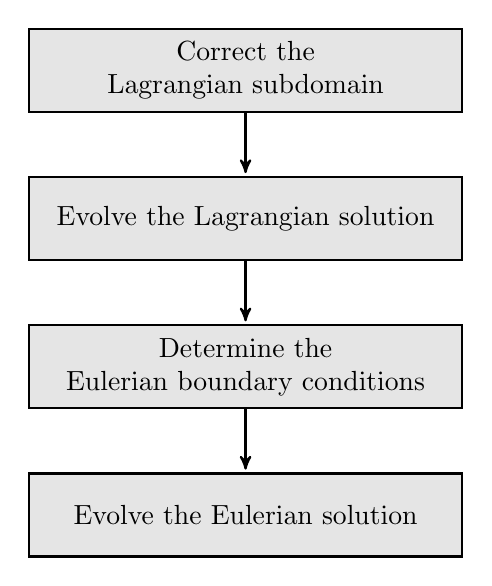
\begin{tikzpicture}
			[node distance=.8cm, start chain=going below,]
			\node[punktchain, join] (correct) {Correct the \\Lagrangian subdomain};
		    \node[punktchain, join] (evolveL) {Evolve the Lagrangian solution};
		    \node[punktchain, join] (bcE)     {Determine the \\Eulerian boundary conditions};
		    \node[punktchain, join] (evolveE) {Evolve the Eulerian solution};
		\end{tikzpicture}
		\caption{Flowchart of the simple coupling strategy. The flowchart shows the procedure to evolve both methods from $t_n$ to $t_{n+1}$.}
		\label{fig:flowchart_simpleCoupling}
	\end{figure}




% Summarize daenincks approach:
	% Methodology, algorithm
	% Domain decomposition
% Summarize stock's approach:
	% Methodology, algorithms
	% Resulted domain decomposition.


%%%%%%%%%%%%%%%%%%%%%%%%%%%%%%%%%%%%%%%%%%%%%%%%%%%%%%%%%%%%%%%%%%%%%%%%%%%%%%%%%%%%%%%%%%%%%%%%%%%%%%%%%%%%%%%%%%%%%%%%%%%%%%%%%%



%
    %\addtocontents{toc}{\protect\setcounter{tocdepth}{0}}
    %\chapter{Feasibility of hybrid vortex method for compressor cascade}
	%\appendixpage
    %\addcontentsline{toc}{chapter}{Appendices}
	%\appendix
	%\addcontentsline{toc}{chapter}{Appendix}
	%\input{appendices/main}

\backmatter%

    % index file here (not needed for a MSc thesis)
	%\printindex
	
\end{document}
